\documentclass[10pt,math=newtx,citestyle=gb7714-2015,bibstyle=gb7714-2015]{elegantbook}

\title{Dynare 4.7:User Guide for Advanced Topics}
%\subtitle{User Guide for Advanced Topics}

\author{Wenddy Xu, Jingru Luo}
\institute{AHU/CIMERS/NEEL, China; SFU, Canada}
\date{July 10, 2021}
\version{0.7}
\bioinfo{Email}{xuweny87@hotmail.com}


\setcounter{tocdepth}{3}

\logo{cimers_logo.jpg}
\cover{cover1.png}

\usepackage{array}
\newcommand{\ccr}[1]{\makecell{{\color{#1}\rule{1cm}{1cm}}}}

\definecolor{customcolor}{RGB}{32,178,170}
\colorlet{coverlinecolor}{customcolor}

\begin{document}
	
	\maketitle
	\frontmatter
	
	\thispagestyle{empty}
	
	\newpage
	
	~\vfill
	
	Copyright  2018-2021 Wenddy Xu
	
	
	\bigskip
	
	Permission is granted to copy, distribute and/or modify this document under the terms of the GNU Free Documentation License, Version 1.3 or any later version published by the Free Software Foundation; with no Invariant Sections, no Front-Cover Texts, and no Back-Cover Texts.
	
	\bigskip
	
	A copy of the license can be found at: \url{http://www.gnu.org/licenses/fdl.txt}
	
	\vfill
	
	\newpage
	
	\chapter*{Work in Progress}
	
	\markboth{Introduction}{Introduction}
	
	
	This is the draft version of the Dynare User Guide for Advanced Topics which is still work in progress! This means three things. First, please read this with a critical eye and send me comments! Are some areas unclear? Is anything plain wrong? Are some sections too wordy, are there enough examples, are these clear? On the contrary, are there certain parts that just click particularly well? How can others be improved? I'm very interested to get your feedback. 
	
	The second thing is that a work in progress manuscript comes with is a few internal notes. These are mostly placeholders for future work, notes to myself or others of the Dynare development team, or at times notes to you - our readers - to highlight a feature not yet fully stable. 
	
	The third thing is regard to the references of my notes. When I had been writing the notes, I copy-paste some contents from many nice papers, so I thanks for the authors's contribution. The reference lists are still work in progress!
	
	Especially, thanks Tommaso Mancini Griffoli for his Dynare User Guide. Meantime, thanks very much for your patience and good ideas. Please write either direclty to myself: xuweny87@hotmail.com, or \textbf{preferably on the Dynare Forum} available in the \href{http://forum.dynare.org}{Dynare Forums}.
	
	
	
	\vskip 1.5cm
	
	\begin{flushright}
		Wenddy Xu\\
		Jun 30, 2018
	\end{flushright}

\chapter*{Contacts and Credits} 
Dynare was originally developed by Michel Juillard in Paris, France. Currently, the development team of Dynare is composed of

\begin{itemize}
	\item Stphane Adjemian \texttt{<stephane.adjemian@univ-lemans.fr>}
	\item Houtan Bastani \texttt{<houtan@dynare.org>}
	\item Michel Juillard \texttt{<michel.juillard@mjui.fr>}
	\item Frdric Karam \texttt{<frederic.karame@univ-lemans.fr>}
	\item Junior Maih \texttt{<junior.maih@gmail.com>}
	\item Ferhat Mihoubi \texttt{<ferhat.mihoubi@cepremap.org>}
	\item George Perendia \texttt{<george@perendia.orangehome.co.uk>}
	\item Johannes Pfeifer \texttt{<jpfeifer@gmx.de>}
	\item Marco Ratto \texttt{<marco.ratto@jrc.ec.europa.eu>}
	\item Sbastien Villemot \texttt{<sebastien@dynare.org>}
\end{itemize}

Several parts of Dynare use or have strongly benefited from publicly available programs by G. Anderson, F. Collard, L. Ingber, O. Kamenik, P. Klein, S. Sakata, F. Schorfheide, C. Sims, P. Soederlind and R. Wouters.

Finally, the development of Dynare could not have come such a long ways withough an active community of users who continually pose questions, report bugs and suggest new features. The help of this community is gratefully acknowledged.

The email addresses above are provided in case you wish to contact any one of the authors of Dynare directly. We nonetheless encourage you to first use the \href{http://forum.dynare.org/}{Dynare forums} to ask your questions so that other users can benefit from them as well; remember, almost no question is specific enough to interest just one person, and yours is not the exception!
	
	\tableofcontents
	
	\mainmatter
	
	\chapter{Introduction}
	
	Welcome to Dynare! 
	
	\section{About this Guide - approach and structure}
	This User Guide \textbf{aims to help you master Dynare}'s main functionalities, from getting started to implementing advanced features. To do so, this Guide is structured around examples and offers practical advice. To root this understanding more deeply, though, this Guide also gives some background on Dynare's algorithms, methodologies and underlying theory. Thus, a secondary function of this Guide is to \textbf{serve as a basic primer} on DSGE model solving and Bayesian estimation. 
	
	This Guide will focus on the most common or useful features of the program, thus emphasizing \textbf{depth over breadth}. The idea is to get you to use 90\% of the program well and then tell you where else to look if you're interested in fine tuning or advanced customization.
	
	This Guide is written mainly for an \textbf{advanced economist} - like a professor, graduate student or central banker - needing a powerful and flexible program to support and facilitate his or her research activities in a variety of fields. The sophisticated computer programmer, on the one hand, or the specialist of computational economics, on the other, may not find this Guide sufficiently detailed. 
	
	We recognize that the 'advanced economist' may be either a beginning or intermediate user of Dynare. This Guide is written to accommodate both. If you're \textbf{new to Dynare}, we recommend starting with chapters \ref{ch:solbase} and \ref{ch:estbase}, which introduce the program's basic features to solve (including running impulse response functions) and estimate DSGE models, respectively. To do so, these chapters lead you through a complete hands-on example, which we recommend following from A to Z, in order to ``\textbf{learn by doing}''. Once you have read these two chapters, you will know the crux of Dynare's functionality and (hopefully!) feel comfortable using Dynare for your own work. At that point, though, you will probably find yourself coming back to the User Guide to skim over some of the content in the advanced chapters to iron out details and potential complications you may run into.
	
	If you're instead an \textbf{intermediate user} of Dynare, you will most likely find the advanced chapters, \ref{ch:soladv} and \ref{ch:estadv}, more appropriate. These chapters cover more advanced features of Dynare and more complicated usage scenarios. The presumption is that you would skip around these chapters to focus on the topics most applicable to your needs and curiosity. Examples are therefore more concise and specific to each feature; these chapters read a bit more like a reference manual.
	
	We also recognize that you probably have had rep\textbackslash{}documentclass[10pt,math=newtx,citestyle=gb7714-2015,bibstyle=gb7714-2015]\{elegantbook\}
	
	\textbackslash{}title\{Dynare 4.7:User Guide for Advanced Topics\}
	\%\textbackslash{}subtitle\{User Guide for Advanced Topics\}
	
	\textbackslash{}author\{Wenddy Xu, Jingru Luo\}
	\textbackslash{}institute\{AHU/CIMERS/NEEL, China; SFU, Canada\}
	\textbackslash{}date\{July 10, 2021\}
	\textbackslash{}version\{0.7\}
	\textbackslash{}bioinfo\{Email\}\{xuweny87@hotmail.com\}
	
	
	\textbackslash{}setcounter\{tocdepth\}\{3\}
	
	\textbackslash{}logo\{cimers\_logo.jpg\}
	\textbackslash{}cover\{cover1.png\}
	
	\textbackslash{}usepackage\{array\}
	\textbackslash{}newcommand\{\textbackslash{}ccr\}[1]\{\textbackslash{}makecell\{\{\textbackslash{}color\{\#1\}\textbackslash{}rule\{1cm\}\{1cm\}\}\}\}
	
	\textbackslash{}definecolor\{customcolor\}\{RGB\}\{32,178,170\}
	\textbackslash{}colorlet\{coverlinecolor\}\{customcolor\}
	
	\textbackslash{}begin\{document\}
	
	\textbackslash{}maketitle
	\textbackslash{}frontmatter
	
	\textbackslash{}thispagestyle\{empty\}
	
	\textbackslash{}newpage
	
	\~{}\textbackslash{}vfill
	
	Copyright  2018-2021 Wenddy Xu
	
	
	\textbackslash{}bigskip
	
	Permission is granted to copy, distribute and/or modify this document under the terms of the GNU Free Documentation License, Version 1.3 or any later version published by the Free Software Foundation; with no Invariant Sections, no Front-Cover Texts, and no Back-Cover Texts.
	
	\textbackslash{}bigskip
	
	A copy of the license can be found at: \textbackslash{}url\{http://www.gnu.org/licenses/fdl.txt\}
	
	\textbackslash{}vfill
	
	\textbackslash{}newpage
	
	\textbackslash{}chapter*\{Work in Progress\}
	
	\textbackslash{}markboth\{Introduction\}\{Introduction\}
	
	
	This is the draft version of the Dynare User Guide for Advanced Topics which is still work in progress! This means three things. First, please read this with a critical eye and send me comments! Are some areas unclear? Is anything plain wrong? Are some sections too wordy, are there enough examples, are these clear? On the contrary, are there certain parts that just click particularly well? How can others be improved? I'm very interested to get your feedback. 
	
	The second thing is that a work in progress manuscript comes with is a few internal notes. These are mostly placeholders for future work, notes to myself or others of the Dynare development team, or at times notes to you - our readers - to highlight a feature not yet fully stable. 
	
	The third thing is regard to the references of my notes. When I had been writing the notes, I copy-paste some contents from many nice papers, so I thanks for the authors's contribution. The reference lists are still work in progress!
	
	Especially, thanks Tommaso Mancini Griffoli for his Dynare User Guide. Meantime, thanks very much for your patience and good ideas. Please write either direclty to myself: xuweny87@hotmail.com, or \textbackslash{}textbf\{preferably on the Dynare Forum\} available in the \textbackslash{}href\{http://forum.dynare.org\}\{Dynare Forums\}.
	
	
	
	\textbackslash{}vskip 1.5cm
	
	\textbackslash{}begin\{flushright\}
	Wenddy Xu\textbackslash{}\textbackslash{}
	Jun 30, 2018
	\textbackslash{}end\{flushright\}
	
	\textbackslash{}chapter*\{Contacts and Credits\} 
	Dynare was originally developed by Michel Juillard in Paris, France. Currently, the development team of Dynare is composed of
	
	\textbackslash{}begin\{itemize\}
	\textbackslash{}item Stphane Adjemian \textbackslash{}texttt\{<stephane.adjemian@univ-lemans.fr>\}
	\textbackslash{}item Houtan Bastani \textbackslash{}texttt\{<houtan@dynare.org>\}
	\textbackslash{}item Michel Juillard \textbackslash{}texttt\{<michel.juillard@mjui.fr>\}
	\textbackslash{}item Frdric Karam \textbackslash{}texttt\{<frederic.karame@univ-lemans.fr>\}
	\textbackslash{}item Junior Maih \textbackslash{}texttt\{<junior.maih@gmail.com>\}
	\textbackslash{}item Ferhat Mihoubi \textbackslash{}texttt\{<ferhat.mihoubi@cepremap.org>\}
	\textbackslash{}item George Perendia \textbackslash{}texttt\{<george@perendia.orangehome.co.uk>\}
	\textbackslash{}item Johannes Pfeifer \textbackslash{}texttt\{<jpfeifer@gmx.de>\}
	\textbackslash{}item Marco Ratto \textbackslash{}texttt\{<marco.ratto@jrc.ec.europa.eu>\}
	\textbackslash{}item Sbastien Villemot \textbackslash{}texttt\{<sebastien@dynare.org>\}
	\textbackslash{}end\{itemize\}
	
	Several parts of Dynare use or have strongly benefited from publicly available programs by G. Anderson, F. Collard, L. Ingber, O. Kamenik, P. Klein, S. Sakata, F. Schorfheide, C. Sims, P. Soederlind and R. Wouters.
	
	Finally, the development of Dynare could not have come such a long ways withough an active community of users who continually pose questions, report bugs and suggest new features. The help of this community is gratefully acknowledged.
	
	The email addresses above are provided in case you wish to contact any one of the authors of Dynare directly. We nonetheless encourage you to first use the \textbackslash{}href\{http://forum.dynare.org/\}\{Dynare forums\} to ask your questions so that other users can benefit from them as well; remember, almost no question is specific enough to interest just one person, and yours is not the exception!
	
	\textbackslash{}tableofcontents
	
	\textbackslash{}mainmatter
	
	\textbackslash{}chapter\{Introduction\}
	
	Welcome to Dynare! 
	
	\textbackslash{}section\{About this Guide - approach and structure\}
	This User Guide \textbackslash{}textbf\{aims to help you master Dynare\}'s main functionalities, from getting started to implementing advanced features. To do so, this Guide is structured around examples and offers practical advice. To root this understanding more deeply, though, this Guide also gives some background on Dynare's algorithms, methodologies and underlying theory. Thus, a secondary function of this Guide is to \textbackslash{}textbf\{serve as a basic primer\} on DSGE model solving and Bayesian estimation. 
	
	This Guide will focus on the most common or useful features of the program, thus emphasizing \textbackslash{}textbf\{depth over breadth\}. The idea is to get you to use 90\textbackslash{}\% of the program well and then tell you where else to look if you're interested in fine tuning or advanced customization.
	
	This Guide is written mainly for an \textbackslash{}textbf\{advanced economist\} - like a professor, graduate student or central banker - needing a powerful and flexible program to support and facilitate his or her research activities in a variety of fields. The sophisticated computer programmer, on the one hand, or the specialist of computational economics, on the other, may not find this Guide sufficiently detailed. 
	
	We recognize that the ``advanced economist'' may be either a beginning or intermediate user of Dynare. This Guide is written to accommodate both. If you're \textbackslash{}textbf\{new to Dynare\}, we recommend starting with chapters \textbackslash{}ref\{ch:solbase\} and \textbackslash{}ref\{ch:estbase\}, which introduce the program's basic features to solve (including running impulse response functions) and estimate DSGE models, respectively. To do so, these chapters lead you through a complete hands-on example, which we recommend following from A to Z, in order to ``\textbackslash{}textbf\{learn by doing\}''. Once you have read these two chapters, you will know the crux of Dynare's functionality and (hopefully!) feel comfortable using Dynare for your own work. At that point, though, you will probably find yourself coming back to the User Guide to skim over some of the content in the advanced chapters to iron out details and potential complications you may run into.
	
	If you're instead an \textbackslash{}textbf\{intermediate user\} of Dynare, you will most likely find the advanced chapters, \textbackslash{}ref\{ch:soladv\} and \textbackslash{}ref\{ch:estadv\}, more appropriate. These chapters cover more advanced features of Dynare and more complicated usage scenarios. The presumption is that you would skip around these chapters to focus on the topics most applicable to your needs and curiosity. Examples are therefore more concise and specific to each feature; these chapters read a bit more like a reference manual.
	
	We also recognize that you probably have had repeated if not active exposure to programming and are likely to have a strong economic background. Thus, a black box solution to your needs is inadequate. To hopefully address this issue, the User Guide goes into some depth in covering the \textbackslash{}textbf\{theoretical underpinnings and methodologies that Dynare follows\} to solve and estimate DSGE models. These are available in the ``behind the scenes of Dynare'' chapters \textbackslash{}ref\{ch:solbeh\} and \textbackslash{}ref\{ch:estbeh\}. These chapters can also serve as a \textbackslash{}textbf\{basic primer\} if you are new to the practice of DSGE model solving and Bayesian estimation. 
	
	Finally, besides breaking up content into short chapters, we've introduced two different \textbackslash{}textbf\{markers\} throughout the Guide to help streamline your reading.
	\textbackslash{}begin\{itemize\}
	\textbackslash{}item \textbackslash{}textbf\{\textbackslash{}textsf\{TIP!\}\} introduces advice to help you work more efficiently with Dynare or solve common problems.
	\textbackslash{}item \textbackslash{}textbf\{\textbackslash{}textsf\{NOTE!\}\} is used to draw your attention to particularly important information you should keep in mind when using Dynare.
	\textbackslash{}end\{itemize\}
	
	
	\textbackslash{}section\{What are the advanced topics?\}
	Before we dive into the thick of the ``trees'', let's have a look at the ``forest'' from the top \textbackslash{}ldots just what is Dynare? 
	
	\textbackslash{}textbf\{Dynare is a powerful and highly customizable engine, with an intuitive front-end interface, to solve, simulate and estimate DSGE models\}. 
	
	In slightly less flowery words, it is a pre-processor and a collection of Matlab routines that has the great advantages of reading DSGE model equations written almost as in an academic paper. This not only facilitates the inputting of a model, but also enables you to easily share your code as it is straightforward to read by anyone.\textbackslash{}\textbackslash{}
	\textbackslash{}begin\{figure\} \textbackslash{}label\{fig:dyn\}
	\textbackslash{}begin\{center\}
	\textbackslash{}includegraphics[width=1.0\textbackslash{}textwidth]\{P\_DynareStruct2\}
	\textbackslash{}end\{center\}
	\textbackslash{}caption[Dynare, a bird's eyeview]\{The .mod file being read by the Dynare pre-processor, which then calls the relevant Matlab routines to carry out the desired operations and display the results.\}
	\textbackslash{}end\{figure\}
	
	Figure \textbackslash{}ref\{fig:dyn\} gives you an overview of the way Dynare works. Basically, the model and its related attributes, like a shock structure for instance, is written equation by equation in an editor of your choice. The resulting file will be called the .mod file. That file is then called from Matlab. This initiates the Dynare pre-processor which translates the .mod file into a suitable input for the Matlab routines (more precisely, it creates intermediary Matlab or C files which are then used by Matlab code) used to either solve or estimate the model. Finally, results are presented in Matlab. Some more details on the internal files generated by Dynare is given in section \textbackslash{}ref\{sec:dynfiles\} in chapter \textbackslash{}ref\{ch:soladv\}. 
	
	Each of these steps will become clear as you read through the User Guide, but for now it may be helpful to summarize \textbackslash{}textbf\{what Dynare is able to do\}:
	\textbackslash{}begin\{itemize\}
	\textbackslash{}item compute the steady state of a model
	\textbackslash{}item compute the solution of deterministic models
	\textbackslash{}item compute the first and second order approximation to solutions of stochastic models
	\textbackslash{}item estimate parameters of DSGE models using either a maximum likelihood or a Bayesian approach
	\textbackslash{}item compute optimal policies in linear-quadratic models
	\textbackslash{}end\{itemize\}
	
	
	\textbackslash{}section\{Additional sources of help\}
	While this User Guide tries to be as complete and thorough as possible, you will certainly want to browse other material for help, as you learn about new features, struggle with adapting examples to your own work, and yearn to ask that one question whose answer seems to exist no-where. At your disposal, you have the following additional sources of help:
	\textbackslash{}begin\{itemize\}
	\textbackslash{}item \textbackslash{}href\{http://www.dynare.org/documentation-and-support/manual\}\{\textbackslash{}textbf\{Reference Manual\}\}: this manual covers all Dynare commands, giving a clear definition and explanation of usage for each. The User Guide will often introduce you to a command in a rather loose manner (mainly through examples); so reading corresponding command descriptions in the Reference Manual is a good idea to cover all relevant details.
	\textbackslash{}item \textbackslash{}href\{http://www.dynare.org/documentation-and-support/examples\}\{\textbackslash{}textbf\{Official online examples\}\}: the Dynare website includes other examples - usually well documented - of .mod files covering models and methodologies introduced in recent papers.
	\textbackslash{}item \textbackslash{}href\{http://www.dynare.org/phpBB3\}\{\textbackslash{}textbf\{Dynare forums\}\}: this lively online discussion forum allows you to ask your questions openly and read threads from others who might have run into similar difficulties.
	\textbackslash{}item \textbackslash{}href\{http://www.dynare.org/documentation-and-support/faq\}\{\textbackslash{}textbf\{Frequently Asked Questions\}\} (FAQ): this section of the Dynare site emphasizes a few of the most popular questions in the forums.
	\textbackslash{}item \textbackslash{}href\{http://www.dsge.net\}\{\textbackslash{}textbf\{DSGE.net\}\}: this website, run my members of the Dynare team, is a resource for all scholars working in the field of DSGE modeling. Besides allowing you to stay up to date with the most recent papers and possibly make new contacts, it conveniently lists conferences, workshops and seminars that may be of interest.
	\textbackslash{}end\{itemize\}
	
	\textbackslash{}section\{Nomenclature\}
	To end this introduction and avoid confusion in what follows, it is worthwhile to agree on a few \textbackslash{}textbf\{definitions of terms\}. Many of these are shared with the Reference Manual.
	\textbackslash{}begin\{itemize\}
	\textbackslash{}item \textbackslash{}textbf\{Integer\} indicates an integer number.
	\textbackslash{}item \textbackslash{}textbf\{Double\} indicates a double precision number. The following syntaxes are valid: 1.1e3, 1.1E3, 1.1E-3, 1.1d3, 1.1D3
	\textbackslash{}item \textbackslash{}textbf\{Expression\} indicates a mathematical expression valid in the underlying language (e.g. Matlab).
	\textbackslash{}item \textbackslash{}textbf\{Variable name\} indicates a variable name. \textbackslash{}textbf\{\textbackslash{}textsf\{NOTE!\}\} These must start with an alphabetical character and can only contain other alphabetical characters and digits, as well as underscores (\textbackslash{}\_). All other characters, including accents, and \textbackslash{}textbf\{spaces\}, are forbidden.
	\textbackslash{}item \textbackslash{}textbf\{Parameter name\} indicates a parameter name which must follow the same naming conventions as above.
	\textbackslash{}item \textbackslash{}textbf\{Filename\} indicates a file name valid in your operating system. Note that Matlab requires that names of files or functions start with alphabetical characters; this concerns your Dynare .mod files.
	\textbackslash{}item \textbackslash{}textbf\{Command\} is an instruction to Dynare or other program when specified.
	\textbackslash{}item \textbackslash{}textbf\{Options\} or optional arguments for a command are listed in square brackets \textbackslash{}mbox\{[ ]\} unless otherwise noted. If, for instance, the option must be specified in parenthesis in Dynare, it will show up in the Guide as [(option)].
	\textbackslash{}item \textbackslash{}textbf\{\textbackslash{}texttt\{Typewritten text\}\} indicates text as it should appear in Dynare code.
	\textbackslash{}end\{itemize\}
	
	\textbackslash{}section\{v4.5, what's new and backward compatibility\}
	The current version of Dynare - for which this guide is written - is version 4.5. With respect to version 4.4, this new version introduces several important features, as well as improvements, optimizations of routines and bug fixes. The major new features are the following:
	\textbackslash{}begin\{itemize\}
	\textbackslash{}item Ramsey policy
	
	
	Added command ramsey\textbackslash{}\_model that builds the expanded model with FOC conditions for the planner's problem but doesn't perform any computation. Useful to compute Ramsey policy in a perfect foresight model and for estimation,
	
	
	ramsey\textbackslash{}\_policy accepts multipliers in its variable list and displays results for them.
	
	\textbackslash{}item Perfect foresight models
	
	
	New commands perfect\textbackslash{}\_foresight\textbackslash{}\_setup (for preparing the simulation) and perfect\textbackslash{}\_foresight\textbackslash{}\_solver (for computing it). The old simul command still exist and is now an alias for perfect\textbackslash{}\_foresight\textbackslash{}\_setup + perfect\textbackslash{}\_foresight\textbackslash{}\_solver. It is no longer possible to manipulate by hand the contents of
	oo\textbackslash{}\_.exo\textbackslash{}\_simul when using simul. People who want to do it must first call perfect\textbackslash{}\_foresight\textbackslash{}\_setup, then do the manipulations, then call perfect\textbackslash{}\_foresight\textbackslash{}\_solver,
	
	
	By default, the perfect foresight solver will try a homotopy method if it fails to converge at the first try. The old behavior can be restored with the no\textbackslash{}\_homotopy option,
	
	
	New option stack\textbackslash{}\_solve\textbackslash{}\_algo=7 that allows specifying a solve\textbackslash{}\_algo solver for solving the model,
	
	
	New option solve\textbackslash{}\_algo that allows specifying a solver for solving the model when using stack\textbackslash{}\_solve\textbackslash{}\_algo=7,
	
	
	New option lmmcp that solves the model via a Levenberg-Marquardt mixed complementarity problem (LMMCP) solver,
	
	
	New option robust\textbackslash{}\_lin\textbackslash{}\_solve that triggers the use of a robust linear solver for the default solve\textbackslash{}\_algo=4,
	
	
	New options tolf and tolx to control termination criteria of solvers,
	
	
	New option endogenous\textbackslash{}\_terminal\textbackslash{}\_period to simul,
	
	
	Added the possibility to set the initial condition of the (stochastic) extended path simulations with the histval block.
	
	\textbackslash{}item Optimal simple rules
	
	
	Saves the optimal value of parameters to oo\textbackslash{}\_.osr.optim\textbackslash{}\_params,
	
	
	New block osr\textbackslash{}\_params\textbackslash{}\_bounds allows specifying bounds for the estimated parameters,
	
	
	New option opt\textbackslash{}\_algo allows selecting different optimizers while the new option optim allows specifying the optimizer options,
	
	
	The osr command now saves the names, bounds, and indices for the estimated parameters as well as the indices and weights of the variables entering the objective function into M\textbackslash{}\_.osr.
	
	\textbackslash{}item Forecasts and Smoothing
	
	
	The smoother and forecasts take uncertainty about trends and means into account,
	
	
	Forecasts accounting for measurement error are now saved in fields of the form HPDinf\textbackslash{}\_ME and HPDsup\textbackslash{}\_ME,
	
	
	New fields oo\textbackslash{}\_.Smoother.Trend and oo\textbackslash{}\_.Smoother.Constant that save the trend and constant parts of the smoothed variables,
	
	
	new field oo\textbackslash{}\_.Smoother.TrendCoeffs that stores the trend coefficients.
	
	
	Rolling window forecasts allowed in estimation command by passing a vector to first\textbackslash{}\_obs,
	
	
	The calib\textbackslash{}\_smoother command now accepts the loglinear, prefilter, first\textbackslash{}\_obs and filter\textbackslash{}\_decomposition options.
	\textbackslash{}item Estimation
	
	
	New options: logdata, consider\textbackslash{}\_all\textbackslash{}\_endogenous,consider\textbackslash{}\_only\textbackslash{}\_observed, posterior\textbackslash{}\_max\textbackslash{}\_subsample\textbackslash{}\_draws, mh\textbackslash{}\_conf\textbackslash{}\_sig, diffuse\textbackslash{}\_kalman\textbackslash{}\_tol, dirname, nodecomposition.
	
	
	load\textbackslash{}\_mh\textbackslash{}\_file and mh\textbackslash{}\_recover now try to load chain's proposal density\textbackslash{},
	
	
	New option load\textbackslash{}\_results\textbackslash{}\_after\textbackslash{}\_load\textbackslash{}\_mh that allows loading some posterior results from a previous run if no new MCMC draws areadded,
	
	
	New option posterior\textbackslash{}\_nograph that suppresses the generation of graphs associated with Bayesian IRFs, posterior smoothed objects, and posterior forecasts,
	
	
	Saves the posterior density at the mode in oo\textbackslash{}\_.posterior.optimization.log\textbackslash{}\_density,
	
	
	The filter\textbackslash{}\_covariance option now also works with posterior sampling like Metropolis-Hastings,
	
	
	New option no\textbackslash{}\_posterior\textbackslash{}\_kernel\textbackslash{}\_density to suppress computation of kernel density of posterior objects,
	
	
	Recursive estimation and forecasting now provides the individual
	oo\textbackslash{}\_ structures for each sample in oo\textbackslash{}\_recursive\textbackslash{}\_,
	
	
	The trace\textbackslash{}\_plot command can now plot the posterior density,
	
	
	New command generate\textbackslash{}\_trace\textbackslash{}\_plots allows generating all trace plots for one chain,
	
	
	New commands prior\textbackslash{}\_function and posterior\textbackslash{}\_function that execute a user-defined function on parameter draws from the prior/posterior distribution ,
	
	
	New option huge\textbackslash{}\_number for replacement of infinite bounds with large number during mode\textbackslash{}\_compute,
	
	
	New option posterior\textbackslash{}\_sampling\textbackslash{}\_method allows selecting the new posterior sampling options: tailored\textbackslash{}\_random\textbackslash{}\_block\textbackslash{}\_metropolis\textbackslash{}\_hastings (Tailored randomized block (TaRB) Metropolis-Hastings), slice (Slice sampler), independent\textbackslash{}\_metropolis\textbackslash{}\_hastings (Independent Metropolis-Hastings).
	
	
	New option posterior\textbackslash{}\_sampler\textbackslash{}\_options that allow controlling the options of the posterior\textbackslash{}\_sampling\textbackslash{}\_method; its scale\textbackslash{}\_file-option pair allows loading the \textbackslash{}\_mh\textbackslash{}\_scale.mat-file storing the tuned scale factor from a previous run of mode\textbackslash{}\_compute=6,
	
	
	New option raftery\textbackslash{}\_lewis\textbackslash{}\_diagnostics that computes Raftery/Lewis (1992) convergence diagnostics,
	
	
	New option fast\textbackslash{}\_kalman\textbackslash{}\_filter that provides fast Kalman filter using Chandrasekhar recursions as described in Ed Herbst (2015),
	
	
	The dsge\textbackslash{}\_var option now saves results at the posterior mode into oo\textbackslash{}\_.dsge\textbackslash{}\_var,
	
	
	New option smoothed\textbackslash{}\_state\textbackslash{}\_uncertainty to provide the uncertainty estimate for the smoothed state estimate from the Kalman smoother,
	
	
	New prior density: generalized Weibull distribution,
	
	
	Option mh\textbackslash{}\_recover now allows continuing a crashed chain at the last save mh-file,
	
	
	New option nonlinear\textbackslash{}\_filter\textbackslash{}\_initialization for the estimation command. Controls the initial covariance matrix of the state variables in nonlinear filters.
	
	
	The conditional\textbackslash{}\_variance\textbackslash{}\_decomposition option now displays output and stores it as a LaTeX-table when the TeX option is invoked,
	
	
	The use\textbackslash{}\_calibration to estimated\textbackslash{}\_params\textbackslash{}\_init now also works with ML,
	
	
	Improved initial estimation checks.
	
	
	
	
	\textbackslash{}item Steady state
	
	
	The default solver for finding the steady state is now a trust-region solver (can be triggered explicitly with option
	solve\textbackslash{}\_algo=4),
	
	
	New options tolf and tolx to control termination criteria of solver,
	
	
	The debugging mode now provides the termination values in steady state finding.
	
	
	
	
	\textbackslash{}item Stochastic simulations
	
	
	New options nodecomposition,
	
	
	New option bandpass\textbackslash{}\_filter to compute bandpass-filtered theoretical and simulated moments,
	
	
	New option one\textbackslash{}\_sided\textbackslash{}\_hp\textbackslash{}\_filter to compute one-sided HP-filtered simulated moments,
	
	
	stoch\textbackslash{}\_simul displays a simulated variance decomposition when simulated moments are requested,
	
	
	stoch\textbackslash{}\_simul saves skewness and kurtosis into respective fields of oo\textbackslash{}\_ when simulated moments have been requested,
	
	
	stoch\textbackslash{}\_simul saves the unconditional variance decomposition in oo\textbackslash{}\_.variance\textbackslash{}\_decomposition,
	
	
	New option dr\textbackslash{}\_display\textbackslash{}\_tol that governs omission of small terms in display of decision rules,
	
	
	The stoch\textbackslash{}\_simul command now prints the displayed tables as LaTeX code when the new TeX option is enabled,
	
	
	The loglinear option now works with lagged and leaded exogenous variables like news shocks,
	
	
	New option spectral\textbackslash{}\_density that allows displaying the spectral density of (filtered) endogenous variables,
	
	
	New option contemporaneous\textbackslash{}\_correlation that allows saving contemporaneous correlations in addition to the covariances.
	
	
	
	
	\textbackslash{}item Identification
	
	
	New options diffuse\textbackslash{}\_filter and prior\textbackslash{}\_trunc,
	
	
	The identification command now supports correlations via simulated moments,
	
	
	
	
	\textbackslash{}item Sensitivity analysis
	
	
	New blocks irf\textbackslash{}\_calibration and moment\textbackslash{}\_calibration,
	
	
	Outputs LaTeX tables if the new TeX option is used,
	
	
	New option relative\textbackslash{}\_irf to irf\textbackslash{}\_calibration block.
	
	
	
	
	\textbackslash{}item Conditional forecast
	
	Command conditional\textbackslash{}\_forecast now takes into account histval block if present.
	
	
	
	\textbackslash{}item Shock decomposition
	
	
	New option colormap to shocks\textbackslash{}\_decomposition for controlling the color map used in the shocks decomposition graphs,
	
	
	shocks\textbackslash{}\_decomposition now accepts the nograph option,
	
	
	New command realtime\textbackslash{}\_shock\textbackslash{}\_decomposition that for each period T= [presample,...,nobs] allows computing the:
	
	
	realtime historical shock decomposition Y(t|T), i.e. without observing data in [T+1,...,nobs]
	
	
	forecast shock decomposition Y(T+k|T)
	
	
	realtime conditional shock decomposition Y(T+k|T+k)-Y(T+k|T)
	
	
	
	
	New block shock\textbackslash{}\_groups that allows grouping shocks for the shock\textbackslash{}\_decomposition and realtime\textbackslash{}\_shock\textbackslash{}\_decomposition commands.
	
	
	New command plot\textbackslash{}\_shock\textbackslash{}\_decomposition that allows plotting the results from shock\textbackslash{}\_decomposition and realtime\textbackslash{}\_shock\textbackslash{}\_decomposition for different vintages and shock groupings.
	
	
	
	
	\textbackslash{}item Macroprocessor
	
	
	Can now pass a macro-variable to the \textbackslash{}@\textbackslash{}\#include macro directive,
	
	
	New preprocessor flag -I, macro directive \textbackslash{}@\textbackslash{}\#includepath, and dynare config file block [paths] to pass a search path to the macroprocessor to be used for file inclusion via \textbackslash{}@\textbackslash{}\#include.
	
	
	
	
	\textbackslash{}item Command line
	
	
	New option onlyclearglobals (do not clear JIT compiled functions with recent versions of Matlab),
	
	
	New option minimal\textbackslash{}\_workspace to use fewer variables in the current workspace,
	
	
	New option params\textbackslash{}\_derivs\textbackslash{}\_order allows limiting the order of the derivatives with respect to the parameters that are calculated by the preprocessor,
	
	
	New command line option mingw to support the MinGW-w64 C/C++ Compiler from TDM-GCC for use\textbackslash{}\_dll.
	
	
	
	
	\textbackslash{}item dates/dseries/reporting classes
	
	
	New methods abs, cumprod and chain,
	
	
	New option tableRowIndent to addTable,
	
	
	Reporting system revamped and made more efficient, dependency on matlab2tikz has been dropped.
	
	
	
	
	\textbackslash{}item Optimization algorithms
	
	
	mode\textbackslash{}\_compute=2 Uses the simulated annealing as described by Corana et al. (1987),
	
	
	mode\textbackslash{}\_compute=101 Uses SOLVEOPT as described by Kuntsevich and Kappel (1997),
	
	
	mode\textbackslash{}\_compute=102 Uses simulannealbnd from Matlab's Global Optimization Toolbox (if available),
	
	
	New option silent\textbackslash{}\_optimizer to shut off output from mode computing/optimization,
	
	
	New options verbosity and SaveFiles to control output and saving of files during mode computing/optimization.
	
	
	
	
	\textbackslash{}item LaTeX output
	
	
	New command write\textbackslash{}\_latex\textbackslash{}\_original\textbackslash{}\_model,
	
	
	New option write\textbackslash{}\_equation\textbackslash{}\_tags to write\textbackslash{}\_latex\textbackslash{}\_dynamic\textbackslash{}\_model that allows printing the specified equation tags to the generate
	LaTeX code,
	
	
	New command write\textbackslash{}\_latex\textbackslash{}\_parameter\textbackslash{}\_table that writes the names and values of model parameters to a LaTeX table,
	
	
	New command write\textbackslash{}\_latex\textbackslash{}\_prior\textbackslash{}\_table that writes the descriptive statistics about the prior distribution to a LaTeX table,
	
	
	New command collect\textbackslash{}\_latex\textbackslash{}\_files that creates one compilable LaTeX file containing all TeX-output.
	
	
	
	
	\textbackslash{}item Misc.
	
	
	Provides 64bit preprocessor,
	
	
	Introduces new path management to avoid conflicts with other toolboxes,
	
	
	Full compatibility with Matlab 2014b's new graphic interface,
	
	
	When using model(linear), Dynare automatically checks whether the model is truly linear,
	
	
	usedll: the msvc option now supports normcdf, acosh, asinh, and atanh,
	
	
	New parallel option NumberOfThreadsPerJob for Windows nodes that sets the number of threads assigned to each remote MATLAB/Octave run,
	
	
	Improved numerical performance of schur\textbackslash{}\_statespace\textbackslash{}\_transformation for very large models,
	
	
	The all\textbackslash{}\_values\textbackslash{}\_required option now also works with histval,
	
	
	Add missing horizon option to ms\textbackslash{}\_forecast,
	
	
	BVAR now saves the marginal data density in oo\textbackslash{}\_.bvar.log\textbackslash{}\_marginal\textbackslash{}\_data\textbackslash{}\_density and stores prior and posterior information in oo\textbackslash{}\_.bvar.prior and oo\textbackslash{}\_.bvar.posterior.
	\textbackslash{}end\{itemize\}
	
	
	
	
	\textbackslash{}chapter\{Installing Dynare\}
	
	\textbackslash{}section\{Dynare versions\}
	
	Dynare runs on both \textbackslash{}href\{http://www.mathworks.com/products/matlab/\}\{\textbackslash{}textbf\{MATLAB\}\} and \textbackslash{}href\{http://www.octave.org\}\{\textbackslash{}textbf\{GNU Octave\}\}.
	
	There used to be versions of Dynare for \textbackslash{}textbf\{Scilab\} and \textbackslash{}textbf\{Gauss\}. Development of the Scilab version stopped after Dynare version 3.02 and that for Gauss after Dynare version 1.2.
	
	This User Guide will exclusively \textbackslash{}textbf\{focus on Dynare version 4.0 and later\}.
	
	You may also be interested by another program, \textbackslash{}textbf\{Dynare++\}, which is a standalone C++ program specialized in computing k-order approximations of dynamic stochastic general equilibrium models. Note that Dynare++ is distributed along with Dynare since version 4.1. See the \textbackslash{}href\{http://www.dynare.org/documentation-and-support/dynarepp\}\{Dynare++ webpage\} for more information. 
	
	\textbackslash{}section\{System requirements\}
	Dynare can run on Microsoft Windows, as well as Unix-like operating systems, in particular GNU/Linux and Mac OS X. If you have questions about the support of a particular platform, please ask your question on \textbackslash{}href\{http://www.dynare.org/phpBB3\}\{\textbackslash{}textbf\{Dynare forums\}\}.
	
	To run Dynare, it is recommended to allocate at least 256MB of RAM to the platform running Dynare, although 512MB is preferred. Depending on the type of computations required, like the very processor intensive Metropolis Hastings algorithm, you may need up to 1GB of RAM to obtain acceptable computational times.
	
	\textbackslash{}section\{Installing Dynare\}
	
	Please refer to the section entitled ``Installation and configuration'' in the \textbackslash{}href\{http://www.dynare.org/documentation-and-support/manual\}\{Dynare reference manual\}.
	
	\textbackslash{}section\{MATLAB particularities\}
	
	A question often comes up: what special MATLAB toolboxes are necessary to run Dynare? In fact, no additional toolbox is necessary for running most of Dynare, except maybe for optimal simple rules (see chapter \textbackslash{}ref\{ch:ramsey\}), but even then remedies exist (see the \textbackslash{}href\{http://www.dynare.org/phpBB3\}\{Dynare forums\} for discussions on this, or to ask your particular question). But if you do have the `optimization toolbox' installed, you will have additional options for solving for the steady state (solve\textbackslash{}\_algo option) and for searching for the posterior mode (mode\textbackslash{}\_compute option), both of which are defined later. 
	
	\textbackslash{}chapter\{Solving Steady State - basics\}
	Basically, you have to remove all the time indices (t-1,t,t+1,...) on the endogenous and exogenous variables in all the equations, and express the endogenous variables as functions of the exogenous variables and parameters. This cannot be done analytically in all models, and often you will have to resort on a numerical solver to obtain the steady state (for given values of the parameters and exogenous variables). This is what Dynare does if you do not provide a closed form expression for the steady state. In small models (basic RBC or NK models), it is possible to obtain an analytical expression for the steady state.
	
	As is known to all, the steady-state value of the DSGE model is very difficult to solve, especially for complex nonlinear models. When we use the DSGE model, usually more than \$80\textbackslash{}\%\$ of the time may be spent on solving the steady-state values of endogenous variables. Doing so borders on a form of art, and luck is unfortunately part of the equation. Therefore, the following methods/skills/steps may be of some help to you.
	
	
	\textbackslash{}section\{Analytical Solutions\} \textbackslash{}label\{sec:distcn\}
	
	First of all, let's look at a simple model.
	
	The equilibrium system of the model is:
	
	\textbackslash{}begin\{equation\}\textbackslash{}label\{label\}
	C\_t\^{}\{\textbackslash{}sigma\}\textbackslash{}theta N\_t\^{}\{\textbackslash{}phi\}=w\_t
	\textbackslash{}end\{equation\}
	
	\textbackslash{}begin\{equation\}\textbackslash{}label\{label\}
	E\_t\textbackslash{}frac\{C\_\{t+1\}\^{}\{\textbackslash{}sigma\}\}\{C\_t\^{}\{\textbackslash{}sigma\}\}=\textbackslash{}beta E\_t(R\_\{t+1\}+(1-\textbackslash{}delta))
	\textbackslash{}end\{equation\}
	
	\textbackslash{}begin\{equation\}\textbackslash{}label\{label\}
	E\_t\textbackslash{}frac\{C\_\{t+1\}\^{}\{\textbackslash{}sigma\}\}\{C\_t\^{}\{\textbackslash{}sigma\}\}=\textbackslash{}beta E\_t(1+r\_t)
	\textbackslash{}end\{equation\}
	
	\textbackslash{}begin\{equation\}\textbackslash{}label\{label\}
	K\_\{t+1\}=I\_t+(1-\textbackslash{}delta)K\_t
	\textbackslash{}end\{equation\}
	
	\textbackslash{}begin\{equation\}\textbackslash{}label\{label\}
	\textbackslash{}alpha A\_tK\_t\^{}\{\textbackslash{}alpha-1\}N\_t\^{}\{1-\textbackslash{}alpha\}=R\_t
	\textbackslash{}end\{equation\}
	
	\textbackslash{}begin\{equation\}\textbackslash{}label\{label\}
	(1-\textbackslash{}alpha)A\_tK\_t\^{}\{\textbackslash{}alpha\}N\_t\^{}\{-\textbackslash{}alpha\}=w\_t
	\textbackslash{}end\{equation\}
	
	\textbackslash{}begin\{equation\}\textbackslash{}label\{label\}
	Y\_t=A\_tK\_t\^{}\{\textbackslash{}alpha\}N\_t\^{}\{1-\textbackslash{}alpha\}
	\textbackslash{}end\{equation\}
	
	\textbackslash{}begin\{equation\}\textbackslash{}label\{label\}
	Y\_t=C\_t+I\_t
	\textbackslash{}end\{equation\}
	
	\textbackslash{}begin\{equation\}\textbackslash{}label\{label\}
	lnA\_t=\textbackslash{}rho lnA\_\{t-1\}+\textbackslash{}epsilon\_t
	\textbackslash{}end\{equation\}
	
	(3.1) is the labor supply equation. (3.2) is the investment-saving equilibrium, which is the capital Euler equation. (3.3) is also the investment-saving equilibrium, which is the bond Euler equation. (3.4) is the capital accumulation equation. (3.5) is the capital demand equation. (3.6) is the labor demand equation. (3.7) is the production function. (3.8) It is the product market clearing. (3.9) is the productivity shock. Among them, there is a lead variable \$C\_\{t+1\}\$, and two state variables \$K\_t,A\_t\$. The model equilibrium system contains 9 endogenous variables \$Y\_t,C\_t,N\_t,K\_t,I\_t,w\_t,R\_t,r\_t,A\_t\$, and 9 equations.
	
	
	The equilibrium of the model has been defined above, and then we will define and solve the steady state of the model. Steady state means that the endogenous variables are equal in each period,\$E\_tx\_\{t+1\}=x\_t=x\_\{t-1\}=x\_\{ss\}\$.
	
	First, in the steady state, remove the time subscripts of all variables. \$E\_t\textbackslash{}epsilon\_t=0\$, therefore, \$A=1\$ can be obtained from the productivity evolution equation (3.9). And in the steady state, \$K\_\{t+1\}=K\_t=K,C\_\{t+1\}=C\_t=C\$.
	
	Starting from Euler's equations (3.2) and (3.3), it is easiest to solve the steady state. 
	
	(1) From (3.2) and (3.3),
	
	\textbackslash{}begin\{equation\}\textbackslash{}label\{label\}
	\textbackslash{}begin\{split\}
	\textbackslash{}beta(R+1-\textbackslash{}delta)=1\textbackslash{}\textbackslash{}
	\textbackslash{}Leftrightarrow R=\textbackslash{}frac\{1\}\{\textbackslash{}beta\}+\textbackslash{}delta-1
	\textbackslash{}end\{split\}
	\textbackslash{}end\{equation\}
	
	\textbackslash{}begin\{equation\}\textbackslash{}label\{label\}
	\textbackslash{}begin\{split\}
	\textbackslash{}beta(1+r)=1\textbackslash{}\textbackslash{}
	\textbackslash{}Leftrightarrow r=\textbackslash{}frac\{1\}\{\textbackslash{}beta\}-1
	\textbackslash{}end\{split\}
	\textbackslash{}end\{equation\}
	
	(2) From the capital demand function (3.5), the steady state of the capital-labor ratio can be solved:
	
	\textbackslash{}begin\{equation\}\textbackslash{}label\{label\}
	\textbackslash{}begin\{split\}
	R=\textbackslash{}alpha(\textbackslash{}frac\{K\}\{N\})\^{}\{\textbackslash{}alpha-1\}\textbackslash{}\textbackslash{}
	\textbackslash{}Leftrightarrow \textbackslash{}frac\{K\}\{N\}=(\textbackslash{}frac\{R\}\{\textbackslash{}alpha\})\^{}\{\textbackslash{}frac\{1\}\{\textbackslash{}alpha-1\}\}\textbackslash{}\textbackslash{}
	\textbackslash{}Leftrightarrow \textbackslash{}frac\{K\}\{N\}=(\textbackslash{}frac\{\textbackslash{}alpha\}\{\textbackslash{}frac\{1\}\{\textbackslash{}beta\}+\textbackslash{}delta-1\})\^{}\{\textbackslash{}frac\{1\}\{1-\textbackslash{}alpha\}\}
	\textbackslash{}end\{split\}
	\textbackslash{}end\{equation\}
	
	Note that the third line of (3.12) is obtained by substituting the result of (3.10) into the second line.
	
	(3)Substituting the capital-labor steady-state ratio of (3.12) into the labor demand equation of (3.6), we get
	
	\textbackslash{}begin\{equation\}\textbackslash{}label\{label\}
	\textbackslash{}begin\{split\}
	w=(1-\textbackslash{}alpha)(\textbackslash{}frac\{K\}\{N\})\^{}\{\textbackslash{}alpha\}\textbackslash{}\textbackslash{}
	\textbackslash{}Leftrightarrow w=(1-\textbackslash{}alpha)(\textbackslash{}frac\{\textbackslash{}alpha\}\{\textbackslash{}frac\{1\}\{\textbackslash{}beta\}+\textbackslash{}delta-1\})\^{}\{\textbackslash{}frac\{\textbackslash{}alpha\}\{1-\textbackslash{}alpha\}\}
	\textbackslash{}end\{split\}
	\textbackslash{}end\{equation\}
	
	(4)From the capital accumulation equation (3.4), we can get \$I=\textbackslash{}delta K\$, and from the production function (3.7), we can get \$Y=(\textbackslash{}frac\{K\}\{N\})\^{}\{\textbackslash{}alpha\}N\$.
	
	(5)Substituting the two formulas in the fourth step into the product market clearing equation (3.8) to obtain
	
	\textbackslash{}begin\{equation\}\textbackslash{}label\{label\}
	\textbackslash{}begin\{split\}
	(\textbackslash{}frac\{K\}\{N\})\^{}\{\textbackslash{}alpha\}N=C+\textbackslash{}delta K\textbackslash{}\textbackslash{}
	\textbackslash{}Leftrightarrow \textbackslash{}frac\{C\}\{N\}=(\textbackslash{}frac\{K\}\{N\})\^{}\{\textbackslash{}alpha\}-\textbackslash{}delta \textbackslash{}frac\{K\}\{N\}
	\textbackslash{}end\{split\}
	\textbackslash{}end\{equation\}
	
	(6)Combining the above equation (3.14) with the labor demand equation (3.13) , and \$\textbackslash{}frac\{K\}\{N\},w\$ is known, thus
	
	\textbackslash{}begin\{equation\}\textbackslash{}label\{label\}
	\textbackslash{}left\textbackslash{}\{
	\textbackslash{}begin\{aligned\}
	C\^{}\{\textbackslash{}sigma\}\textbackslash{}theta N\_t\^{}\{\textbackslash{}phi\}=w\textbackslash{}\textbackslash{}
	\textbackslash{}frac\{C\}\{N\}=(\textbackslash{}frac\{K\}\{N\})\^{}\{\textbackslash{}alpha\}-\textbackslash{}delta \textbackslash{}frac\{K\}\{N\}\textbackslash{}\textbackslash{}
	\textbackslash{}end\{aligned\}
	\textbackslash{}right.
	\textbackslash{}end\{equation\}
	
	Through the above equation (3.15), the steady-state value of consumption and labor \$C,N\$ can be solved. Once the steady state of labor \$N\$ is obtained, it can be substituted into the steady state of capital-labor ratio (3.12) to solve the steady state of capital \$K\$, and then the steady state of output and investment \$Y,I\$ can be obtained.
	
	For small scale DSGE models, we can find analytical solutions for each endogenous variable. Therefore, the accurate steady-state values can be obtained. However, because Dynare is more sensitive to the initial values, it may still report an error at this time. So we need to add some optimization options after the steady command:
	
	\textbackslash{}begin\{itemize\}
	\textbackslash{}item \$solve\textbackslash{}\_algo=0:\$ Use the fsolve function in the Optimization Toolbox in Matlab.
	\textbackslash{}item \$solve\textbackslash{}\_algo=1:\$ Use the Dynare built-in nonlinear equation algorithm.
	\textbackslash{}item \$solve\textbackslash{}\_algo=2:\$ Divide the model into recursive modules and solve each module one by one.
	\textbackslash{}item \$solve\textbackslash{}\_algo=3:\$ Use the Sims algorithm. This is the default option.
	\textbackslash{}end\{itemize\}
	
	\textbackslash{}section\{Adding new variable one by one\}
	
	Analytical methods are generally applicable to small-scale DSGE models.  However, the analytical solutions are difficult to be solved for medium and large scale models. Fortunately, the DSGE model is very modular, and the complex models are basically extended based on the baseline model (small scale). Therefore, we can gradually introduce the sectors or factors we are interested in to expand to new models. For example, in the RBC model, the monopolistic competition structure of enterprises is introduced first, and then the price stickiness of intermediate product enterprises is introduced, thus forming the New Keynesian model.
	
	This idea of adding factors step by step also provides an idea for us to solve the steady state. That is to say, when we solve the steady state, we also follow the path of \$baseline model - extended model 1 - extended model 2 - \textbackslash{}cdots - final model \$.
	
	For example, in the RBC model of the previous section, we introduced the monopolistic competition factor, then the equilibrium system becomes:
	
	\textbackslash{}begin\{equation\}\textbackslash{}label\{label\}
	C\_t\^{}\{\textbackslash{}sigma\}\textbackslash{}theta N\_t\^{}\{\textbackslash{}phi\}=w\_t
	\textbackslash{}end\{equation\}
	
	\textbackslash{}begin\{equation\}\textbackslash{}label\{label\}
	E\_t\textbackslash{}frac\{C\_\{t+1\}\^{}\{\textbackslash{}sigma\}\}\{C\_t\^{}\{\textbackslash{}sigma\}\}=\textbackslash{}beta E\_t(R\_\{t+1\}+(1-\textbackslash{}delta))
	\textbackslash{}end\{equation\}
	
	\textbackslash{}begin\{equation\}\textbackslash{}label\{label\}
	E\_t\textbackslash{}frac\{C\_\{t+1\}\^{}\{\textbackslash{}sigma\}\}\{C\_t\^{}\{\textbackslash{}sigma\}\}=\textbackslash{}beta E\_t(1+r\_t)
	\textbackslash{}end\{equation\}
	
	\textbackslash{}begin\{equation\}\textbackslash{}label\{label\}
	K\_\{t+1\}=I\_t+(1-\textbackslash{}delta)K\_t
	\textbackslash{}end\{equation\}
	
	\textbackslash{}begin\{equation\}\textbackslash{}label\{label\}
	\textbackslash{}alpha MC\_t A\_tK\_t\^{}\{\textbackslash{}alpha-1\}N\_t\^{}\{1-\textbackslash{}alpha\}=R\_t
	\textbackslash{}end\{equation\}
	
	\textbackslash{}begin\{equation\}\textbackslash{}label\{label\}
	(1-\textbackslash{}alpha)MC\_t A\_tK\_t\^{}\{\textbackslash{}alpha\}N\_t\^{}\{-\textbackslash{}alpha\}=w\_t
	\textbackslash{}end\{equation\}
	
	\textbackslash{}begin\{equation\}\textbackslash{}label\{label\}
	Y\_t=A\_tK\_t\^{}\{\textbackslash{}alpha\}N\_t\^{}\{1-\textbackslash{}alpha\}
	\textbackslash{}end\{equation\}
	
	\textbackslash{}begin\{equation\}\textbackslash{}label\{label\}
	Y\_t=C\_t+I\_t
	\textbackslash{}end\{equation\}
	
	\textbackslash{}begin\{equation\}\textbackslash{}label\{label\}
	MC\_t=\textbackslash{}frac\{\textbackslash{}xi\_t-1\}\{\textbackslash{}xi\_t\}
	\textbackslash{}end\{equation\}
	
	\textbackslash{}begin\{equation\}\textbackslash{}label\{label\}
	lnA\_t=\textbackslash{}rho lnA\_\{t-1\}+\textbackslash{}epsilon\_t
	\textbackslash{}end\{equation\}
	
	\textbackslash{}begin\{equation\}\textbackslash{}label\{label\}
	ln\textbackslash{}xi \_t=(1-\textbackslash{}rho\_\{\textbackslash{}xi\})ln\textbackslash{}xi+\textbackslash{}rho\_\{\textbackslash{}xi\} ln\textbackslash{}xi\_\{t-1\}+\textbackslash{}epsilon\_\{\textbackslash{}xi\}
	\textbackslash{}end\{equation\}
	
	The equilibrium system includes 10 endogenous variables \$Y\_t,C\_t,N\_t,K\_t,I\_t,w\_t,R\_t,r\_t,MC\_t,A\_t,\textbackslash{}xi\_t\$, and 10 equations.
	
	
	\textbackslash{}textbf\{Steady State\}
	
	The equilibrium of the model has been defined above, and in the following we will define and solve the steady state of the model. Steady state means that the endogenous variables are equal in each period, \$E\_tx\_\{t+1\}=x\_t=x\_\{t-1\}=x\_\{ss\}\$. Firstly, at steady state, the time subscripts of all variables are removed. \$E\_t\textbackslash{}epsilon\_t=0\$. Therefore, \$A=1\$ can be obtained from the productivity evolution equation (3.25). In additional, at the steady state, \$K\_\{t+1\}=K\_t=K, C\_\{t+1\}=C\_t=C\$.
	
	The steady state is easiest to be solved by starting with Euler's equations (3.17) and (3.18).
	
	(1) \~{} From (3.17) and (3.18), we can get that
	
	\textbackslash{}begin\{equation\}\textbackslash{}label\{label\}
	\textbackslash{}begin\{split\}
	\textbackslash{}beta(R+1-\textbackslash{}delta)=1\textbackslash{}\textbackslash{}
	\textbackslash{}Leftrightarrow R=\textbackslash{}frac\{1\}\{\textbackslash{}beta\}+\textbackslash{}delta-1
	\textbackslash{}end\{split\}
	\textbackslash{}end\{equation\}
	
	\textbackslash{}begin\{equation\}\textbackslash{}label\{label\}
	\textbackslash{}begin\{split\}
	\textbackslash{}beta(1+r)=1\textbackslash{}\textbackslash{}
	\textbackslash{}Leftrightarrow r=\textbackslash{}frac\{1\}\{\textbackslash{}beta\}-1
	\textbackslash{}end\{split\}
	\textbackslash{}end\{equation\}
	
	(2)\~{}The steady state of the capital-labor ratio can be solved from the capital demand function (3.20):
	
	\textbackslash{}begin\{equation\}\textbackslash{}label\{label\}
	\textbackslash{}begin\{split\}
	R=\textbackslash{}alpha MC(\textbackslash{}frac\{K\}\{N\})\^{}\{\textbackslash{}alpha-1\}\textbackslash{}\textbackslash{}
	\textbackslash{}Leftrightarrow \textbackslash{}frac\{K\}\{N\}=(\textbackslash{}frac\{R\}\{\textbackslash{}alpha MC\})\^{}\{\textbackslash{}frac\{1\}\{\textbackslash{}alpha-1\}\}\textbackslash{}\textbackslash{}
	\textbackslash{}Leftrightarrow \textbackslash{}frac\{K\}\{N\}=(\textbackslash{}frac\{\textbackslash{}alpha MC\}\{\textbackslash{}frac\{1\}\{\textbackslash{}beta\}+\textbackslash{}delta-1\})\^{}\{\textbackslash{}frac\{1\}\{1-\textbackslash{}alpha\}\}
	\textbackslash{}end\{split\}
	\textbackslash{}end\{equation\}
	
	Note that the third line of (3.27) is obtained by substituting the result of (3.25) into the second line.
	
	(3)\~{}According to the capital-labor steady-state ratio of (3.27), substituting it into the labor demand equation of (3.21), we get:
	
	\textbackslash{}begin\{equation\}\textbackslash{}label\{label\}
	\textbackslash{}begin\{split\}
	w=(1-\textbackslash{}alpha)(\textbackslash{}frac\{K\}\{N\})\^{}\{\textbackslash{}alpha\}\textbackslash{}\textbackslash{}
	\textbackslash{}Leftrightarrow w=(1-\textbackslash{}alpha)(\textbackslash{}frac\{\textbackslash{}alpha MC\}\{\textbackslash{}frac\{1\}\{\textbackslash{}beta\}+\textbackslash{}delta-1\})\^{}\{\textbackslash{}frac\{\textbackslash{}alpha\}\{1-\textbackslash{}alpha\}\}
	\textbackslash{}end\{split\}
	\textbackslash{}end\{equation\}
	
	(4)\~{}From the capital accumulation equation (3.19), we know that \$I=\textbackslash{}delta K\$, and from the production function (3.22), we know that \$Y=(\textbackslash{}frac\{K\}\{N\})\^{}\{\textbackslash{}alpha\}N\$.
	
	(5)\~{}Substituting the two equations in the fourth step into the product market clearing equation (3.23), we get
	
	\textbackslash{}begin\{equation\}\textbackslash{}label\{label\}
	\textbackslash{}begin\{split\}
	(\textbackslash{}frac\{K\}\{N\})\^{}\{\textbackslash{}alpha\}N=C+\textbackslash{}delta K\textbackslash{}\textbackslash{}
	\textbackslash{}Leftrightarrow \textbackslash{}frac\{C\}\{N\}=(\textbackslash{}frac\{K\}\{N\})\^{}\{\textbackslash{}alpha\}-\textbackslash{}delta \textbackslash{}frac\{K\}\{N\}
	\textbackslash{}end\{split\}
	\textbackslash{}end\{equation\}
	
	(6)\~{}Combining the above equation (3.29) with the labor demand equation (3.16), and \$\textbackslash{}frac\{K\}\{N\},w\$ is known, we get
	
	\textbackslash{}begin\{equation\}\textbackslash{}label\{label\}
	\textbackslash{}left\textbackslash{}\{
	\textbackslash{}begin\{aligned\}
	C\^{}\{\textbackslash{}sigma\}\textbackslash{}theta N\_t\^{}\{\textbackslash{}phi\}=w\textbackslash{}\textbackslash{}
	\textbackslash{}frac\{C\}\{N\}=(\textbackslash{}frac\{K\}\{N\})\^{}\{\textbackslash{}alpha\}-\textbackslash{}delta \textbackslash{}frac\{K\}\{N\}\textbackslash{}\textbackslash{}
	\textbackslash{}end\{aligned\}
	\textbackslash{}right.
	\textbackslash{}end\{equation\}
	
	The steady state value of consumption and labor \$C,N\$ can be solved by the above equation (3.29). Once the steady state of labor \$N\$ is obtained, it can be substituted into the capital-labor ratio steady state (3.27) to solve the capital steady state \$K\$, and then obtain the output and investment steady state \$Y,I\$.
	
	(7)\~{}The marginal cost steady state MC can be solved by the price mark-up shocks (3.26) and (3.24).
	
	
	For another example, we introduce the price stickiness factor in the above extended model. Then we can get the following equilibrium system:
	
	\textbackslash{}begin\{equation\}\textbackslash{}label\{label\}
	C\_t\^{}\{\textbackslash{}sigma\}\textbackslash{}theta N\_t\^{}\{\textbackslash{}phi\}=w\_t
	\textbackslash{}end\{equation\}
	
	\textbackslash{}begin\{equation\}\textbackslash{}label\{label\}
	E\_t\textbackslash{}frac\{C\_\{t+1\}\^{}\{\textbackslash{}sigma\}\}\{C\_t\^{}\{\textbackslash{}sigma\}\}=\textbackslash{}beta E\_t(R\_\{t+1\}+(1-\textbackslash{}delta))
	\textbackslash{}end\{equation\}
	
	\textbackslash{}begin\{equation\}\textbackslash{}label\{label\}
	E\_t\textbackslash{}frac\{C\_\{t+1\}\^{}\{\textbackslash{}sigma\}\}\{C\_t\^{}\{\textbackslash{}sigma\}\}=\textbackslash{}beta E\_t(1+r\_t)
	\textbackslash{}end\{equation\}
	
	\textbackslash{}begin\{equation\}\textbackslash{}label\{label\}
	K\_\{t+1\}=I\_t+(1-\textbackslash{}delta)K\_t
	\textbackslash{}end\{equation\}
	
	\textbackslash{}begin\{equation\}\textbackslash{}label\{label\}
	\textbackslash{}frac\{\textbackslash{}alpha\}\{1-\textbackslash{}alpha\} \textbackslash{}frac\{N\_t\}\{K\_t\}=\textbackslash{}frac\{R\_t\}\{w\_t\}
	\textbackslash{}end\{equation\}
	
	\textbackslash{}begin\{equation\}\textbackslash{}label\{label\}
	Y\_tv\_t\^{}p=A\_tK\_t\^{}\{\textbackslash{}alpha\}N\_t\^{}\{1-\textbackslash{}alpha\}
	\textbackslash{}end\{equation\}
	
	\textbackslash{}begin\{equation\}\textbackslash{}label\{label\}
	Y\_t=C\_t+I\_t
	\textbackslash{}end\{equation\}
	
	\textbackslash{}begin\{equation\}\textbackslash{}label\{label\}
	MC\_t=\textbackslash{}frac\{w\_t\}\{(1-\textbackslash{}alpha)A\_t(\textbackslash{}frac\{K\_t\}\{N\_t\})\^{}\{\textbackslash{}alpha\}\}\textbackslash{}frac\{\textbackslash{}xi-1\}\{\textbackslash{}xi\}
	\textbackslash{}end\{equation\}
	
	\textbackslash{}begin\{equation\}\textbackslash{}label\{label\}
	lnA\_t=\textbackslash{}rho lnA\_\{t-1\}+\textbackslash{}epsilon\_t
	\textbackslash{}end\{equation\}
	
	\textbackslash{}begin\{equation\}\textbackslash{}label\{label\}
	v\_t\^{}p=(1-\textbackslash{}phi)(1+\textbackslash{}pi\_t\^{}\{\textbackslash{}star\})\^{}\{-\textbackslash{}xi\}(1+\textbackslash{}pi\_t)\^{}\{\textbackslash{}xi\}+(1+\textbackslash{}pi\_t)\^{}\{\textbackslash{}xi\}\textbackslash{}phi v\_\{t-1\}\^{}p
	\textbackslash{}end\{equation\}
	
	\textbackslash{}begin\{equation\}\textbackslash{}label\{label\}
	(1+\textbackslash{}pi\_t)\^{}\{1-\textbackslash{}xi\}=(1-\textbackslash{}phi)(1+\textbackslash{}pi\_t\^{}\{\textbackslash{}star\})\^{}\{1-\textbackslash{}xi\}+\textbackslash{}phi
	\textbackslash{}end\{equation\}
	
	\textbackslash{}begin\{equation\}\textbackslash{}label\{label\}
	1+\textbackslash{}pi\_t\^{}\{\textbackslash{}star\}=\textbackslash{}frac\{\textbackslash{}xi\}\{\textbackslash{}xi-1\}(1+\textbackslash{}pi\_t)\textbackslash{}frac\{x\_\{1t\}\}\{x\_\{2t\}\}
	\textbackslash{}end\{equation\}
	
	\textbackslash{}begin\{equation\}\textbackslash{}label\{label\}
	x\_\{1t\}=C\_t\^{}\{-\textbackslash{}sigma\}MC\_tY\_t+\textbackslash{}phi \textbackslash{}beta E\_t(1+\textbackslash{}pi\_\{t+1\})\^{}\{\textbackslash{}xi\}x\_\{1,t+1\}
	\textbackslash{}end\{equation\}
	
	\textbackslash{}begin\{equation\}\textbackslash{}label\{label\}
	x\_\{2t\}=C\_t\^{}\{-\textbackslash{}sigma\}Y\_t+\textbackslash{}phi \textbackslash{}beta E\_t(1+\textbackslash{}pi\_\{t+1\})\^{}\{\textbackslash{}xi-1\}x\_\{2,t+1\}
	\textbackslash{}end\{equation\}
	
	\textbackslash{}begin\{equation\}\textbackslash{}label\{label\}
	r\_t=(1-\textbackslash{}rho\_r)r+\textbackslash{}rho\_rr\_\{t-1\}+(1-\textbackslash{}rho\_r)(\textbackslash{}phi\_\{\textbackslash{}pi\}(\textbackslash{}pi\_t-\textbackslash{}pi)+\textbackslash{}phi\_y(lnY\_t-lnY))+\textbackslash{}epsilon\_t
	\textbackslash{}end\{equation\}
	
	The equilibrium system includes 15 endogenous variables \$Y\_t,C\_t,N\_t,K\_t,I\_t,w\_t,R\_t,r\_t,MC\_t,A\_t,v\_t\^{}p,\textbackslash{}pi\_t,\textbackslash{}pi\_t\^{}\{\textbackslash{}star\},x\_\{1t\},x\_\{2t\}\$, and 15 equations.
	
	
	\textbackslash{}textbf\{Steady State\}
	
	First, we can solve \$\textbackslash{}pi\$ from (3.47);
	Then, we substitute \$\textbackslash{}pi\$ into (3.43), and solve \$\textbackslash{}pi\^{}\{\textbackslash{}star\}\$;
	
	From(3.45) and (3.46), we can get
	\$\$MC=\textbackslash{}frac\{x\_\{1\}\}\{x\_\{2\}\}\textbackslash{}frac\{1-\textbackslash{}phi \textbackslash{}beta(1+\textbackslash{}pi)\^{}\{\textbackslash{}xi\}\}\{1-\textbackslash{}phi \textbackslash{}beta(1+\textbackslash{}pi)\^{}\{\textbackslash{}xi-1\}\}\$\$
	
	Once we know the steady state of MC, we can go back to (3.29) to solve the steady state of \$\textbackslash{}frac\{K\}\{N\}\$, and then solve the steady state values of other endogenous variables in turn.
	
	Exercise: The model that introducing fiscal policy.
	
	
	\textbackslash{}section\{Calibrating Steady State\}
	
	Calibrating steady state? We seem to have only heard of calibrating parameters. In fact, both are the same.
	
	Parameter calibration seems to be the most ‘despised’ but must-use method. However, what I want to say is that this method was used by the ancestors of econometrics when the Econometric Society was founded, and it is the cornerstone of all subsequent estimation methods.
	
	Kydland and Prescott (1982) used a method to convert the DSGE model they analyzed into an empirical analysis. The method they use is a calibration exercise. DeJong and Dave (2007) call this approach the basis of MM/ML/BL.
	
	We know that under the criticism of Lucas (1976) and Sims (1980), the estimation and hypothesis testing of probabilistic methods are not applicable to structural models. Therefore, the goal of the calibration exercise is to explore some specific quantitative problem with a parametric structural model. Kydland and Prescott (1991,, SJE; 1996, JEP) trace the historical origins of calibration linkages as an empirical research method, which you can read. Paragraph one of the constitution elaborated upon the motto by stating that the object of the Society should be to.promote studies that aim at a unification of the theoretical-quantitative and the empirical-quantitative approach to economic problems and that are penetrated by constructive and rigorous thinking similar to that which has come to dominate in the natural sciences. Any activitywhich promises ultimately to further such unification of theoretical and factual studies in economicshall be within the sphere of interest of the Society. ()Frisch(1933a))
	
	Moreover, Frisch (1933b) also used microdata to calibrate production technical parameters and to study the propagation mechanism of business cycle shocks. We all acknowledge that this approach has some flaws, especially with regard to model misspecification. However, as Prescott (1986) points out:
	‘The models constructed within this theoretical framework are necessarily highly abstract. Consequently, they are necessarily false, and statistical hypothesis testing will reject them. This does not imply, however, that nothing can be Learned from such quantitative theoretical exercises. I think much has already been learned and confidently predict that much more will be learned as other features of the environment are introduced. Prime candidates for study are the effects of public finance elements, a foreign sector, and, of course, monetary factors. The researchI review here is best viewed as a very promising beginning of a much larger research program.’
	
	In conclusion, calibration exercises are certainly an empirical tool (DeJong and Dave, 2007). Kydland and Prescott (1996, JEP) stated: ’It is important to note that calibration is not intended to obtain the magnitude of certain parameters, i.e. it is not an estimate.‘ \textbackslash{}textcolor\{red\}\{Therefore, when calibrating DSGE parameters, it usually comes from two aspects: one is the long-term mean; the other is the empirical results of micro-evidence. (For example, Cooley and Prescott (1995) used the microscopic evidence of Ghez and Becker (1975) to calibrate the parameters)\}.
	
	The latter method, which we often use, is generally found in previous research results. However, after the financial crisis, more and more scholars use micro-data/micro-econometric models to estimate relevant parameters of key characteristics in their articles.
	
	The steady state is a mapping between endogenous variables and the parameters of the model. To calibrate a model, we somehow revert this mapping, expressing parameters as function of steady state ratios. For instance, in the Solow model, we have the law of motion for the physical capital stock:
	
	\$\$K\_\{t+1\}=(1-\textbackslash{}delta)K\_t+I\_t\$\$
	
	at the steady state we must have:
	
	\$\$K\^{}\{\textbackslash{}star\}=(1-\textbackslash{}delta)K\^{}\{\textbackslash{}star\}+I\^{}\{\textbackslash{}star\}\$\$
	
	\$\$\textbackslash{}delta K\^{}\{\textbackslash{}star\}=I\^{}\{\textbackslash{}star\}\$\$
	
	hence we know that the depreciation rate must be such that:
	
	\$\$\textbackslash{}delta=\textbackslash{}frac\{I\^{}\{\textbackslash{}star\}\}\{K\^{}\{\textbackslash{}star\}\}\$\$
	
	If we have long time series on physical capital and investment we can then calibrate the depreciation rate with average of the investment/capital ratio. Not all the parameters can be deduced from steady state considerations, since not all parameters will affect the steady state (rigidity parameters for instance). In this case we will have to consider other moments to calibrate these parameters.
	
	Next, let's take a look at how to use the long-term mean/data moment to obtain the steady-state value of the model endogenous variable.
	
	For example, Introduction to Modeling and Programming for DSGE (41): Financial Intermediation
	
	The steady state system is as follows:
	
	\textbackslash{}begin\{equation\}\textbackslash{}label\{label\}
	\textbackslash{}frac\{1\}\{c\_t\}=\textbackslash{}frac\{\textbackslash{}gamma\}\{d\_t\}+\textbackslash{}beta E\_t\textbackslash{}frac\{1+r\_t\^{}d\}\{c\_\{t+1\}\}
	\textbackslash{}end\{equation\}
	
	\textbackslash{}begin\{equation\}\textbackslash{}label\{label\}
	h\_tl\_t\^{}\{\textbackslash{}phi\}=\textbackslash{}frac\{w\_t\}\{c\_t\}
	\textbackslash{}end\{equation\}
	
	\textbackslash{}begin\{equation\}\textbackslash{}label\{label\}
	y\_t=a\_tk\_\{t-1\}\^{}\{\textbackslash{}alpha\}l\_t\^{}\{1-\textbackslash{}alpha\}
	\textbackslash{}end\{equation\}
	
	\textbackslash{}begin\{equation\}\textbackslash{}label\{label\}
	r\_t\^{}k=\textbackslash{}alpha a\_tk\_\{t-1\}\^{}\{\textbackslash{}alpha-1\}l\_t\^{}\{1-\textbackslash{}alpha\}
	\textbackslash{}end\{equation\}
	
	\textbackslash{}begin\{equation\}\textbackslash{}label\{label\}
	w\_t=(1-\textbackslash{}alpha)a\_tk\_\{t-1\}\^{}\{\textbackslash{}alpha\}l\_t\^{}\{-\textbackslash{}alpha\}
	\textbackslash{}end\{equation\}
	
	\textbackslash{}begin\{equation\}\textbackslash{}label\{label\}
	k\_t=m\_t\^{}c+m\_t\^{}s
	\textbackslash{}end\{equation\}
	
	\textbackslash{}begin\{equation\}\textbackslash{}label\{label\}
	m\_t\^{}s=(1-\textbackslash{}kappa)ABS\_t
	\textbackslash{}end\{equation\}
	
	\textbackslash{}begin\{equation\}\textbackslash{}label\{label\}
	(1-\textbackslash{}kappa)E\_t(1+r\_\{t+1\}\^{}k-\textbackslash{}delta)=1+r\_t\^{}a
	\textbackslash{}end\{equation\}
	
	\textbackslash{}begin\{equation\}\textbackslash{}label\{label\}
	m\_t\^{}c+ABS\_t=d\_t+n\_t
	\textbackslash{}end\{equation\}
	
	\textbackslash{}begin\{equation\}\textbackslash{}label\{label\}
	n\_t=\textbackslash{}hat\{\textbackslash{}omega\}m\_t\^{}c
	\textbackslash{}end\{equation\}
	
	\textbackslash{}begin\{equation\}\textbackslash{}label\{label\}
	\textbackslash{}omega\_t=\textbackslash{}hat\{\textbackslash{}omega\}\^{}\{1-\textbackslash{}rho\_\{\textbackslash{}omega\}\}\textbackslash{}omega\_\{t-1\}\^{}\{\textbackslash{}rho\_\{\textbackslash{}omega\}\}\textbackslash{}left(\textbackslash{}frac\{i\_t/i\_\{t-1\}\}\{gdp\_t/gpd\_\{t-1\}\}\textbackslash{}right)\^{}\{\textbackslash{}Phi(1-\textbackslash{}rho\_\{\textbackslash{}omega\})\}e\^{}\{\textbackslash{}epsilon\_\{\textbackslash{}omega,t\}\}
	\textbackslash{}end\{equation\}
	
	\textbackslash{}begin\{equation\}\textbackslash{}label\{label\}
	C(g\_t)=-p\_1ln(1+p\_2g\_t)
	\textbackslash{}end\{equation\}
	
	\textbackslash{}begin\{equation\}\textbackslash{}label\{label\}
	F(\textbackslash{}frac\{ABS\_t\}\{m\_t\^{}c\})=\textbackslash{}frac\{\textbackslash{}phi\}\{2\}\textbackslash{}left(\textbackslash{}frac\{ABS\_t\}\{m\_t\^{}c\}-\textbackslash{}frac\{ABS\}\{m\^{}c\}\textbackslash{}right)\^{}2
	\textbackslash{}end\{equation\}
	
	\textbackslash{}begin\{equation\}\textbackslash{}label\{label\}
	1+C\^{}\{'\}=\textbackslash{}beta E\_t\textbackslash{}frac\{c\_t\}\{c\_\{t+1\}\}(1+r\_t\^{}d)
	\textbackslash{}end\{equation\}
	
	\textbackslash{}begin\{equation\}\textbackslash{}label\{label\}
	(1+s\_t)+(1-\textbackslash{}omega\_t)C\^{}\{'\}-F\^{}\{'\}\textbackslash{}frac\{ABS\_t\}\{(m\_t\^{}c)\^{}2\}=\textbackslash{}beta E\_t\textbackslash{}frac\{c\_t\}\{c\_\{t+1\}\}(1+r\_\{t+1\}\^{}k-\textbackslash{}delta)
	\textbackslash{}end\{equation\}
	
	\textbackslash{}begin\{equation\}\textbackslash{}label\{label\}
	1+C\^{}\{'\}+F\^{}\{'\}\textbackslash{}frac\{1\}\{m\_t\^{}c\}=\textbackslash{}beta E\_t\textbackslash{}frac\{c\_t\}\{c\_\{t+1\}\}(1-P\_\{t+1\})(1+r\_t\^{}a)
	\textbackslash{}end\{equation\}
	
	\textbackslash{}begin\{equation\}\textbackslash{}label\{label\}
	s\_t=\textbackslash{}rho\_ss\_\{t-1\}+\textbackslash{}epsilon\_\{s,t\}
	\textbackslash{}end\{equation\}
	
	\textbackslash{}begin\{equation\}\textbackslash{}label\{label\}
	P\_t=\textbackslash{}rho\_pP\_\{t-1\}+\textbackslash{}epsilon\_\{p,t\}
	\textbackslash{}end\{equation\}
	
	\textbackslash{}begin\{equation\}\textbackslash{}label\{label\}
	lna\_t=\textbackslash{}rho\_alna\_\{t-1\}+\textbackslash{}epsilon\_\{a,t\}
	\textbackslash{}end\{equation\}
	
	\textbackslash{}begin\{equation\}\textbackslash{}label\{label\}
	lnh\_t=(1-\textbackslash{}rho\_h)h+\textbackslash{}rho\_hh\_\{t-1\}+\textbackslash{}epsilon\_\{h,t\}
	\textbackslash{}end\{equation\}
	
	\textbackslash{}begin\{equation\}\textbackslash{}label\{label\}
	y\_t=c\_t+i\_t+C(g\_t)+F(\textbackslash{}frac\{ABS\_t\}\{m\_t\^{}c\})+s\_tm\_t\^{}c+\textbackslash{}kappa ABS\_t
	\textbackslash{}end\{equation\}
	
	\textbackslash{}begin\{equation\}\textbackslash{}label\{label\}
	gdp\_t=c\_t+i\_t
	\textbackslash{}end\{equation\}
	
	\textbackslash{}begin\{equation\}\textbackslash{}label\{label\}
	share\_t=\textbackslash{}frac\{m\_t\^{}s\}\{k\_t\}
	\textbackslash{}end\{equation\}
	
	\textbackslash{}begin\{equation\}\textbackslash{}label\{label\}
	leverage\_t=\textbackslash{}frac\{m\_t\^{}c+ABS\_t\}\{n\_t\}
	\textbackslash{}end\{equation\}
	
	The macroeconomic indicators used include nominal GDP, GDP deflator, nominal net exports, nominal total consumption, CPI, employment, total shadow banking loans, total social financing, treasury bond repurchase rate, labor income share, fixed asset investment, Commercial bank capital adequacy ratio, etc. All are quarterly data.
	
	The macroeconomic indicators used include nominal GDP, GDP deflator, nominal net exports, nominal total consumption, CPI, employment, total shadow banking loans, total social financing, treasury bond repurchase rate, labor income share, fixed asset investment, Commercial bank capital adequacy ratio, etc. All are quarterly data.
	
	The period of labor income share data is Q1 1996 - Q4 2017. The period of fixed asset investment data is Q1 1992- Q4 2017. The period of GDP deflator, nominal net exports, nominal total consumption, CPI, employment, total shadow banking loans, and total social financing is Q1 2002 -Q4 2017. The above data are all from the Chinese macroeconomic database from Chang et al. (2015), Higgins and Tao Zha (2016). The period of nominal GDP is Q1 1992 - Q4 2017, and the data comes from the database of the National Bureau of Statistics of China. The period of the treasury bond repurchase rate is Q1 2000 - Q4 2017, and the data comes from the China Economic Database. The period of the capital adequacy ratio of commercial banks is Q1 2009 - Q4 2017. The data comes from the website of the China Banking Regulatory Commission.
	
	In the above data, the nominal value is all deflated by the relevant price index to obtain the actual value. Since the model economy in this paper does not include the foreign sector, net exports are deducted from GDP to obtain the GDP observations used in this paper. The shadow banking share observations used in this paper are obtained by dividing total shadow banking loans by total social financing. In addition to GDP observations and shadow banking shares, real consumption, employment, and Treasury repurchase rates are used for Bayesian estimation of some parameters of the model. Among them, GDP, consumption, employment, and shadow banking share are all processed by seasonal adjustment, logarithmic difference and mean removal processing, and the treasury bond repurchase rate is seasonally adjusted and mean removal.
	
	Data on other macroeconomic variables are used to calibrate model parameters.
	
	
	\textbackslash{}begin\{figure\}[htbp!]
	\textbackslash{}centering
	\textbackslash{}includegraphics[width=0.8\textbackslash{}linewidth]\{FIG/table1\}
	\textbackslash{}centering
	\textbackslash{}end\{figure\}
	
	
	\textbackslash{}section\{The External Files of Solving Steady State\}
	
	Refer to DSGE Modeling and Programming: Medium-scale DSGE and its code
	
	
	\textbackslash{}chapter\{Occasionally Binding Constraints\}
	
	After the 2008 financial crisis, central banks around the world lowered interest rates to resist the economic downturn, which also brought nominal interest rates down/close to the zero lower bound in various countries. At the same time, households, firms, and financial institutions are also constrained by their own financing constraints due to falling asset prices. And ZLB and financing constraints are the most famous examples of OBCs.
	
	Occasionally binding constraints are part of the economic landscape: for instance recent experience with the global financial crisis has highlighted the gravity of the lower bound constraint on interest rates; emerging economies have been affected by sudden stops, or slowdowns in private capital inflows, that occur from time to time; mortgagors are subject
	to more stringent borrowing conditions when credit growth has been excessive or there is a downturn in the economy; workers have an aversion to taking pay cuts, a problem that is more acute during economic downturns.
	
	The problem of modelling occasionally binding constraints is not a new one. The RBC and DSGE literatures have addressed these problems using a range of different methodologies. These include: eternally binding constraints, smooth approximation of occasionally binding constraints, the extended path algorithm, piecewise linear methods, anticipated shocks, global solution methods, and regime-switching methods.
	
	\textbackslash{}section\{OBCs in Macroeconomics\} \textbackslash{}label\{sec:modsetup\}
	
	OBCs imply that the model is nonlinear in nature, and thus, it also brings computational challenges for DSGE simulation and estimation. I have explained the characteristics of OBCs in DSGE many times in past tweets, such as DSGE Modeling and Programming Introduction (44): ZLB and News Shocks, [Add Dynare code] ZLB+OBC (Occasionally Binding Constraints), DSGE Modeling Getting Started with Programming (36): Financial Friction (3) et al.
	
	One of the simplest and most straightforward approaches to handling occasionally binding constraints is to assume that the constraint is binding at all times. Following Brzoza-Brzezina et al. (2015), we refer to this approach as eternally binding constraints (EBC). Eternally binding constraints are commonly used in the modelling of borrowing and collateral constraints as demonstrated by Iacoviello (2005) and Kiyotaki and Moore (1997). In order to pursue this strategy, the Blanchard-Kahn conditions need to hold when the constraint is binding. While this is a reasonable strategy to pursue for some problems, like the modelling of borrowing constraints, it is not readily applicable to problems like the zero lower bound, which does not in isolation, satisfy the Blanchard-Kahn conditions and is genuinely an occasionally binding constraint that would be poorly approximated as an eternally binding constraint.
	
	Others have tried to solve occasionally binding constraints using smooth approximations. In particular Den Haan and De Wind (2012) propose using an exponential penalty function to prevent negative asset positions in a Deaton-type model. Brzoza-Brzezina et al. (2015) use the same type of penalty function to model occasionally binding collateral constraints.Kim and Ruge-Murcia (2011) use Linex adjustment costs to model downward nominal wage rigidities. While the use of smooth functions permits the use of derivatives, the effective application of these methods requires non-linear solution techniques in order to preserve the non-linearity and asymmetry introduced by the occasionally-binding constraint. When it comes to implementability, smooth approximations work well when the constraint is ``soft'', that is agents can violate the constraint but at some cost.
	
	A range of non-linear solution techniques have been used to solve models with occasionally binding constraints. One of the oldest and most commonly used methods is the extended path algorithm due to Fair and Taylor (1983). The extended path algorithm is a certainty equivalent
	method that solves for the paths of all variables numerically, assuming perfect foresight at each point in time. It has been used by Coenen et al. (2007), Adjemian and Juillard (2010) and Braun and Kober (2011) to account for the zero lower bound on interest rates. A stochastic
	version by Adjemian and Juillard (2013) has been used to model irreversible investment in a DSGE model. While this method can be applied to a range of different occasionally binding constraints, certainty equivalence means agents' behavior does not change in the vicinity of
	the constraint binding. In fact the constraint only impacts agents' behavior when it binds.
	
	Piecewise linear methods have been developed by Jung et al. (2005), Cagliarini and Kulish(2013) and Guerrieri and Iacoviello (2015b) to model occasionally binding constraints. Guerrieri and Iacoviello (2015b), Eggertsson and Woodford (2003) and Braun et al. (2015) have used these methods to enforce the lower bound constraint on interest rates. Guerrieri and Iacoviello (2015a) and Akinci and Queralt (2014) have used piecewise linear methods to account for occasionally binding collateral constraints in DSGE models. Amano and Gnocchi (2017) model downward nominal wage rigidities as a non-negativity constraint on wage inflation and solve the model using piecewise linear methods. While this method is simple and applicable to a range of different occasionally binding constraints, it suffers from some of the same problems as the extended path algorithm, namely that agents' behavior does not change in the vicinity of the constraint binding.
	
	Occasionally binding constraints can also be imposed through the addition of shocks. More specifically Holden and Paetz (2012) have proposed the use of news shocks to impose borrowing constraints and the lower bound on interest rates, while Linde et al. (2016) have used anticipated shocks to enforce the lower bound on interest rates.\textbackslash{}footnote\{1Anticipated shocks differ from the alternative approach commonly referred to as news shocks in many ways. Solving the model with anticipated shocks does not require a modification of the equations of the original system, in contrast to news shocks that are typically implemented by augmenting the law of motion of a shock process with additional shocks. An anticipated shock is genuinely a particular structural shock in the original system, while in the news shocks, it is a different iid shock with no other interpretation than a news shock and is unrelated to any structural shock in the system. Because it is unrelated, it will have its own distribution independently of other parts of the system. Under the anticipated shocks approach the policy functions are explicitly expressed in terms of leads of future shocks as opposed to lags in the news shocks approach (Maih, 2015).\} This method can suffer from sign reversals and the forward guidance puzzle.\textbackslash{}footnote\{Binning and Maih (2016a) describe sign reversals as:... a phenomenon that occurs when anticipated monetary policy shocks are used to enforce the lower bound constraint. In the face of large negative demand shocks, the [effective lower bound (ELB)] is generally seen as a contractionary monetary policy since the interest rate is not able to decrease any further in order to give a boost to the economy. In that case, the anticipated shocks required to keep the interest rate from going below its lower bound are also expected to be positive. The positive monetary policy shocks then act as contractionary policy shocks. In some cases, however, if the ELB is expected to last for a very long time, some of the shocks in the sequence of shocks required to keep the interest rate at the ELB may be negative. Negative monetary policy shocks are expansionary, which leads to an improvement of economic conditions at the ELB.\} \textbackslash{}footnote\{The forward guidance puzzle describes a situation where anticipated monetary policy shocks have a larger than reasonable impact on the current period due to the lack of discounting on the shocks themselves in the consumption Euler equation.\}Just like the extended path and piecewise linear methods, agents are unaware of the constraint until it is actually binding. Moreover the Kuhn-Tucker and complementary slackness conditions associated with many occasionally binding constraints are not easily incorporated into this methodology.\textbackslash{}footnote\{Estimation using these methods requires specialized filters (see Juillard and Maih, 2010).\}
	
	Many practitioners have used global and projection methods to account for occasionally binding constraints. Fernandez-Villaverde et al. (2015) and Judd et al. (2012), among others, have used global methods to impose the lower bound on interest rates. Christiano and Fisher(2000) have used global methods to enforce the non-negativity constraint on investment. Mendoza and Smith (2004) use value function iteration to solve a model with an occasionally binding debt constraint. These methods are certainty non-equivalent which means agents' behavior will be affected in the neighborhood of the constraint binding even when the constraint is not binding. The computational cost of these methods can be heavy putting a low upper bound on the size of models that can be solved.\textbackslash{}footnote\{Estimation requires non-linear filters which further restrict model size.\}
	
	Regime-switching can also be used to impose occasionally binding constraints. Bianchi and Melosi (2014), Chen (2014), Binning and Maih (2016b) and Binning and Maih (2016a) all use regime-switching to impose the lower bound constraint on interest rates. Benigno et al.(2015) use regime-switching to model an occasionally binding debt constraint in a small open economy model. Many occasionally binding constraints involve a policy aspect: the entry and exit of the zero lower bound are functions of the monetary policy regime, debt and collateral constraints can be affected by macroprudential policies like variable loan-to-value ratios. A desirable feature of any solution technique in such an environment is that it be robust to the Lucas critique: regime-switching methods exhibit such a feature.
	
	Four types of OBCs (Occasionally Binding Constraints) in DSGE are discussed in more detail in the User Guide for Advanced Topics:
	
	\textbackslash{}begin\{itemize\}
	\textbackslash{}item Household/Firm borrowing constraints (including CIA, etc.);
	
	\textbackslash{}item Irreversible investment
	
	\textbackslash{}item ZLB
	
	\textbackslash{}item Other financial constraints
	\textbackslash{}end\{itemize\}
	
	\textbackslash{}subsection\{Borrowing Constraints\}
	
	In representative Ricardian and non-Ricardian household models, borrowing constraints always hold.(For example,Iacoviello and Neri (2010)). Guerrieri and Iacoviello (2017) relaxed this assumption and studied how unequal borrowing constraints drive macroeconomic asymmetric dynamics.
	
	Mechanism:
	\textbackslash{}begin\{itemize\}
	\textbackslash{}item During the housing boom, borrowing constraints were loosened as the value of households' mortgages rose;
	
	\textbackslash{}item Housing prices collapsed, the value of household collateral rapidly depreciated, and lending constraints tightened;
	
	\textbackslash{}item This leads to further economic downturns and a downward spiral.
	\textbackslash{}end\{itemize\}
	
	
	Model:
	
	The optimization problem of the Ricardian family with the ratio \$0<\textbackslash{}lambda<1\$ is
	
	\textbackslash{}begin\{equation\}\textbackslash{}label\{label\}
	\textbackslash{}underbrace\{max\}\_\{c\_t\^{}p,h\_t\^{}p,b\_t\^{}p\}\~{}E\_0\textbackslash{}sum\_\{t=0\}\^{}\{\textbackslash{}infty\}\textbackslash{}beta\^{}\{p,t\}u(c\_t\^{}p,h\_t\^{}p)
	\textbackslash{}end\{equation\}
	
	\textbackslash{}begin\{equation\}\textbackslash{}label\{label\}
	c\_t\^{}p+q\_th\_t\^{}p+b\_t\^{}p=y\_t\^{}p+(1-\textbackslash{}delta)q\_th\_\{t-1\}\^{}p+r\_\{t-1\}b\_\{t-1\}
	\textbackslash{}end\{equation\}
	Among them, \$q\_t\$ represents the house price, and \$h\^{}p\$ represents the housing holdings.
	FOCs:
	
	\textbackslash{}begin\{equation\}\textbackslash{}label\{label\}
	u\^{}\{'\}(h\_t\^{}p)=q\_tu\^{}\{'\}(c\_t\^{}p)-\textbackslash{}beta\^{}p(1-\textbackslash{}delta)E\_t[q\_\{t+1\}u\^{}\{'\}(c\_\{t+1\}\^{}p)]
	\textbackslash{}end\{equation\}
	
	\textbackslash{}begin\{equation\}\textbackslash{}label\{label\}
	1=\textbackslash{}beta\^{}pE\_t\textbackslash{}left[\textbackslash{}frac\{u\^{}\{'\}(c\_\{t+1\}\^{}p)\}\{u\^{}\{'\}(c\_\{t\}\^{}p)\}\textbackslash{}right]r\_t
	\textbackslash{}end\{equation\}
	
	The optimization problem for the \$1-\textbackslash{}lambda\$ non-Ricardian family is similar to the Ricardian family above, except that there is an additional borrowing constraint:
	
	\textbackslash{}begin\{equation\}\textbackslash{}label\{label\}
	b\_t\^{}i\textbackslash{}le mq\_th\_t\^{}i
	\textbackslash{}end\{equation\}
	
	At this point, the FOCs of non-Ricardian families:
	
	\textbackslash{}begin\{equation\}\textbackslash{}label\{label\}
	u\^{}\{'\}(h\_t\^{}i)=q\_tu\^{}\{'\}(c\_t\^{}i)-\textbackslash{}beta\^{}i(1-\textbackslash{}delta)E\_t[q\_\{t+1\}u\^{}\{'\}(c\_\{t+1\}\^{}i)]-\textbackslash{}rho\_tq\_tm
	\textbackslash{}end\{equation\}
	
	\textbackslash{}begin\{equation\}\textbackslash{}label\{label\}
	\textbackslash{}rho\_t=u\^{}\{'\}(c\_\{t\}\^{}i)-\textbackslash{}beta\^{}iE\_t\textbackslash{}left[u\^{}\{'\}(c\_\{t+1\}\^{}i)\textbackslash{}right]r\_t
	\textbackslash{}end\{equation\}
	
	where \$\textbackslash{}rho\_t\$ represents the Lagrange multiplier of the borrowing constraint:
	
	\textbackslash{}begin\{equation\}\textbackslash{}label\{label\}
	\textbackslash{}rho\_t\textbackslash{}ge0
	\textbackslash{}end\{equation\}
	
	\textbackslash{}begin\{equation\}\textbackslash{}label\{label\}
	\textbackslash{}rho\_t(mq\_th\_t\^{}i-b\_t\^{}i)=0
	\textbackslash{}end\{equation\}
	
	\textbackslash{}subsection\{Irreversible Investment\}
	
	In reality, at least some of the investment is irreversible, for example if economic conditions change significantly so that the investment becomes a sunk cost.
	
	At this point, then, there is no such opportunity cost of investment in the Standard Model, which would cause uncertainty effects.
	
	Mechanism:
	\textbackslash{}begin\{enumerate\}
	\textbackslash{}item When a firm invests, it observes the future state distribution:
	\textbackslash{}begin\{itemize\}
	\textbackslash{}item In good economic conditions, companies invest more;
	\textbackslash{}item In the worst case, the company will reduce investment;
	\textbackslash{}end\{itemize\}
	\textbackslash{}item As the variance of the future state distribution rises, so does the uncertainty:
	\textbackslash{}begin\{itemize\}
	\textbackslash{}item Higher uncertainty, higher probability to reduce investment;
	\textbackslash{}end\{itemize\}
	\textbackslash{}item Under irreversible investment,
	\textbackslash{}begin\{itemize\}
	\textbackslash{}item cause rms to insure against this be waiting to invest;
	\textbackslash{}item Increase the threshold value of positive investment, i.e. rms will need to see higher expected returns from a project in order to invest.
	\textbackslash{}end\{itemize\}
	\textbackslash{}end\{enumerate\}
	
	Firm production function:
	\textbackslash{}begin\{equation\}\textbackslash{}label\{label\}
	Y\_t=A\_tf(K\_\{t-1\})
	\textbackslash{}end\{equation\}
	
	Capital evolution equation:
	\textbackslash{}begin\{equation\}\textbackslash{}label\{label\}
	K\_t=I\_t+(1-\textbackslash{}delta)K\_\{t-1\}
	\textbackslash{}end\{equation\}
	
	Firms either invest or pay dividends to maximize the intertemporal discounted utility of shareholders.
	
	\textbackslash{}begin\{equation\}\textbackslash{}label\{label\}
	\textbackslash{}underbrace\{max\}\_\{I\_t,D\_t\}\~{}E\_t\textbackslash{}sum\_\{s=0\}\^{}\{\textbackslash{}infty\}\textbackslash{}beta\^{}\{s\}u(D\_\{t+s\})
	\textbackslash{}end\{equation\}
	
	\textbackslash{}begin\{equation\}\textbackslash{}label\{label\}
	D\_t+I\_t=A\_tf(K\_\{t-1\})
	\textbackslash{}end\{equation\}
	
	\textbackslash{}begin\{equation\}\textbackslash{}label\{label\}
	K\_t=I\_t+(1-\textbackslash{}delta)K\_\{t-1\}
	\textbackslash{}end\{equation\}
	
	\textbackslash{}begin\{equation\}\textbackslash{}label\{label\}
	I\_t\textbackslash{}ge0
	\textbackslash{}end\{equation\}
	
	Then, the Lagrangian formula is
	
	\textbackslash{}begin\{equation\}\textbackslash{}label\{label\}
	\textbackslash{}underbrace\{max\}\_\{K\_t\}\~{}E\_t\textbackslash{}sum\_\{s=0\}\^{}\{\textbackslash{}infty\}[\textbackslash{}beta\^{}\{s\}u(A\_\{t+s\}f(K\_\{t+s-1\})-K\_\{t+s\}+(1-\textbackslash{}delta)K\_\{t+s-1\})+\textbackslash{}lambda\_\{t+s\}(K\_\{t+s\}-(1-\textbackslash{}delta)K\_\{t+s-1\})]
	\textbackslash{}end\{equation\}
	
	where  \$\textbackslash{}lambda\_t\textbackslash{}ge0\$ represents the Lagrange multiplier of positive investment. So, FOCs:
	
	\textbackslash{}begin\{equation\}\textbackslash{}label\{label\}
	E\_t\textbackslash{}left[\textbackslash{}beta u'(D\_\{t+1\})(A\_\{t+1\}f'(K\_t)+1-\textbackslash{}delta)\textbackslash{}right]+\textbackslash{}lambda\_t-E\_t[\textbackslash{}lambda\_\{t+1\}](1-\textbackslash{}delta)=u'(D\_t)
	\textbackslash{}end\{equation\}
	
	Note: For any time, as long as \$\textbackslash{}lambda\_t=0\$, the following formula always holds:
	
	\textbackslash{}begin\{equation\}\textbackslash{}label\{label\}
	E\_t\textbackslash{}left[\textbackslash{}beta \textbackslash{}frac\{u'(D\_\{t+1\})\}\{u'(D\_t)\}(A\_\{t+1\}f'(K\_t)+1-\textbackslash{}delta)\textbackslash{}right]=1
	\textbackslash{}end\{equation\}
	
	The above formula is the capital Euler equation in the standard RBC model.
	
	The Lagrange multiplier \$\textbackslash{}lambda\_t\$ can be defined as the shadow price that relaxes the positive investment constraint.
	\textbackslash{}begin\{itemize\}
	\textbackslash{}item If \$I\_t\$ is positive, then \$\textbackslash{}lambda\_t\$ is strictly equal to 0;
	\textbackslash{}item If \$I\_t=0\$, then \$\textbackslash{}lambda\_t\textbackslash{}ge0\$;
	\textbackslash{}item If the state of the economy is such that investment is constrained at 0, then \$E\_t[\textbackslash{}lambda\_\{t+1\}]>0\$.
	\textbackslash{}end\{itemize\}
	
	Assuming \$I\_t>0\$, the FOCs become
	\textbackslash{}begin\{equation\}\textbackslash{}label\{label\}
	E\_t\textbackslash{}left[\textbackslash{}beta u'(D\_\{t+1\})(A\_\{t+1\}f'(K\_t)+1-\textbackslash{}delta)\textbackslash{}right]-E\_t[\textbackslash{}lambda\_\{t+1\}](1-\textbackslash{}delta)=u'(D\_t)
	\textbackslash{}end\{equation\}
	
	If the standard assumption (\$f'>0, f''<0\$) holds, then \textbackslash{}textbf\{non-zero \$E\_t[\textbackslash{}lambda\_\{t+1\}]\$ means that, relative to unconstrained investment, the marginal product of constrained investment is higher, which also means that relative investment is lower.
	
	
	Related laterature:
	
	Caballero and Pindyck (1996) 、Bloom, Bond and Van Reenen (2007) 、Gilchrist, Sim and Zakrajsek (2014) 、Bernanke (1983), Caballero ad Pindyck (1996), Bloom,Bond and Van Reenen (2007), Gilchrist, Sim and Zakrajsek (2014)。
	
	
	\textbackslash{}subsection\{ZLB\}
	
	In the standard NK model (Introduction to DSGE Modeling and Programming (29): NK, Procedures, and Outcomes), monetary policy is typically expressed in response to deviations from target inflation and the target output gap (Introduction to DSGE Modeling and Programming (31): Optimal monetary policy (1)). And the nominal interest rate is 0 as the lower bound, because money has a storage function, therefore, rational people holding money cannot accept negative nominal interest rates. This is called the Zero Lower Bound (ZLB).
	
	However, after the global financial crisis, many central banks around the world are challenging this proposition, successively adjusting the nominal interest rate to around 0, or even setting it to a negative interest rate. Walsh (2017) pointed out in his ``Monetary Theory and Policy'' that if holding money has a certain cost, then people may be willing to accept a certain degree of negative interest rates. Therefore, we should not take it literally as nominal interest rates peg to 0. The most essential understanding should be that nominal interest rates are not sensitive to changes in economic conditions. Walsh (2017) called this phenomenon the ``Effective Lower Bound (ELB)''.
	
	The importance of the ELB issue is reflected in at least two aspects: first, the nonlinear effect represented by the ELB; second, the policy implications: the space for monetary policy to operate is limited, and how the fiscal policy responds.
	
	That is, monetary policy in the benchmark NK model becomes:
	
	\textbackslash{}begin\{equation\}\textbackslash{}label\{label\}
	r\_t=
	\textbackslash{}begin\{cases\}
	(1-\textbackslash{}rho\_r)r+\textbackslash{}rho\_rr\_\{t-1\}+(1-\textbackslash{}rho\_r)(\textbackslash{}phi\_\{\textbackslash{}pi\}(\textbackslash{}pi\_t-\textbackslash{}pi)+\textbackslash{}phi\_y(lnY\_t-lnY))+\textbackslash{}epsilon\_t\~{}\~{}if >0\textbackslash{}\textbackslash{}
	0,\~{}otherwise
	\textbackslash{}end\{cases\}
	\textbackslash{}end\{equation\}
	
	\textbackslash{}begin\{enumerate\}
	\textbackslash{}item Multiple equilibria
	
	Whilst the uniqueness of equilibria can be guaranteed in the standard model by choice of parameters, this is not obviously true when interest rates are constrained at zero.
	\textbackslash{}begin\{itemize\}
	\textbackslash{}item Many methods used to solve models with ZLB choose equilibrium path arbitrarily: When the constraint binds, a return path to long-run steady state is looked for with no check whether solution is unique (we'll see more specifically how in a bit)
	\textbackslash{}item Some papers recognise and discuss the many equilibrium paths
	\textbackslash{}item Other papers discuss multiple steady states/regimes.
	\textbackslash{}end\{itemize\}
	
	Consider standard 3-equation NK model:
	
	implies two long-run equilibria that depend on which agents expect:
	
	1. Normal/inflationary: \$r=\textbackslash{}hat\{r\},\textbackslash{}pi=\textbackslash{}pi\^{}\{star\}\$;
	
	2. Deflationary: \$r=0,\textbackslash{}pi=-r\$.
	
	Non-fundamental (i.e. not to do with technology, output etc) shifts in expectations can cause economy to jump between equilibria (sunspots).
	
	\textbackslash{}item Indeterminacy
	
	Being in the deflationary equilibrium implies that agents believe that the economy is converging to the bad steady-state:
	\textbackslash{}begin\{itemize\}
	\textbackslash{}item Many papers rule this out explicitly both on theoretical and empirical grounds.
	\textbackslash{}end\{itemize\}
	
	It turns out under many specifications, the model is still indeterminate when ZLB binds, even in good equilibrium.
	\textbackslash{}begin\{itemize\}
	\textbackslash{}item Holden (2017) provides necessary and sufficient conditions for determinacy.
	\textbackslash{}item There is a unique equilibrium under a price-level targeting regime rather than inflation targeting regime.
	\textbackslash{}end\{itemize\}
	
	\textbackslash{}item Fiscal multipliers
	
	A number of papers claim that the fiscal multiplier is large when the ZLB binds.
	
	Other papers claim that the fiscal multiplier is only about 1---i.e. no multiplier!
	\textbackslash{}end\{enumerate\}
	
	\textbackslash{}subsection\{Financial Constraints\}
	
	Another set of OBCs in the literature is on either firm financing or financial intermediation.
	
	For further reading see:
	
	\textbackslash{}begin\{itemize\}
	\textbackslash{}item Adverse selection in investment: Swarbrick (2018).
	\textbackslash{}item Bank borrowing constraints: Holden, Levine and Swarbrick (2016).
	\textbackslash{}item Equity constraints: Brunnermeier and Sannikov (2014), He and Krishnamurthy(2013).
	\textbackslash{}item Cash in advance constraints: Dixon and Pourpourides (2016).
	
	\textbackslash{}end\{itemize\}
	
	\textbackslash{}section\{Numerical Solutions\}
	
	\textbackslash{}subsection\{Computational Challenges\}
	
	For example, to solve a DSGE model means solving equations of the form:
	
	\$\$1=\textbackslash{}beta E\_t\textbackslash{}left[\textbackslash{}frac\{u'(c\_\{t+1\})\}\{u'(c\_t)\}R\_\{t+1\}\textbackslash{}right]\$\$
	
	where \$c\_t=f(s\_t,k\_\{t-1\},k\_t)\$, that is 
	\textbackslash{}begin\{itemize\}
	\textbackslash{}item The decisions of agents depend on the current economic state st and the past state \$k\_\{t-1\}\$, and satisfy the above Euler equation;
	
	\textbackslash{}item We finally want to solve the policy function \$k\_t=g(s\_t,k\_\{t-1\})\$, which means \$c\_t=f(s\_t,k\_\{t-1\},g(s\_t,k\_\{t- 1\}))\$;
	
	\textbackslash{}item It is almost impossible to find an analytical solution to the policy function \$g()\$, so function approximation must be used to obtain its approximate form.
	\textbackslash{}end\{itemize\}
	
	So what method can be used to approximate \$g()\$?
	
	Method 1: Use a global approach to approximate the policy function g, that is, in a very large state space (\$s\_t, all possible values of k\_\{t-1\}\$) to obtain a nonlinear approximation function \$g'()=g ()\$:
	\textbackslash{}begin\{itemize\}
	\textbackslash{}item This method is easy to characterize OBCs;
	
	\textbackslash{}item However, the computation is very time consuming and thus limited to smaller models (smaller state space).
	\textbackslash{}end\{itemize\}
	
	Method 2: Perturbation method (local approximation method), that is, to approximate the model near a fixed point (usually a deterministic steady state):
	\textbackslash{}begin\{itemize\}
	\textbackslash{}item Fast and accurate;
	
	\textbackslash{}item When solving the model at a fixed point, if the constraint holds, it will always holds, and if the constraint does not hold, then it will not hold at all the time. (Note: It is especially obvious in the OccBin method)
	\textbackslash{}end\{itemize\}
	
	
	In terms of global algorithm, there are projection method and penalty function method, and these methods all need to write their own programs.
	
	The main drawback of the global solution methods is that
	
	\textbackslash{}begin\{itemize\}
	\textbackslash{}item models solved using global techniques do not scale well to larger models;
	\textbackslash{}item the majority of model solved using this method make restrictive assumptions to limit the state space, such as using exogenous endowment instead of an endogenous production sector;
	\textbackslash{}item Global methods also cannot guarantee convergence for non-optimal problems such as the Taylor rule with a ZLB;
	\textbackslash{}item require a high level of technical skill to set-up.
	\textbackslash{}end\{itemize\}
	
	
	We only explain the local algorithms available to Dynare below.
	\textbackslash{}subsection\{Penalty Function\}
	Perturbation methods cannot directly be applied to models
	with occasionally-binding inequality constraints. In order to deal with the nonnegativity
	constraint for asset holdings, we replace the borrowing constraint by a
	penalty function (Judd [10], pp. 123). The basic idea of this approach is that we
	allow anything to be feasible, but we change the objective function so that it has
	undesirable consequences if the constraints are violated. By using this approach
	we have converted the original problem, given in expression (1) into an optimization
	problem with only equality constraints, which allows us to apply a standard
	perturbation method. Recent contributions that use this approach for heterogeneous
	agents models include Kim et al. [11] and Preston and Roca [16]. There are
	many ways to represent the penalty function. We focus on three specifications from
	the recent literature on heterogeneous agents models. We will use the specification
	described in den Haan and de Wind [8]
	
	\textbackslash{}subsection\{OccBin in Dynare\}
	
	Let's introduce Iacoviello's OccBin algorithm and its operation. As far as I know, the OccBin method is one of the most popular OBCs solutions in the world.
	
	\textbackslash{}textbf\{I. Basic idea\}
	
	The scientific name of the OccBin algorithm is the ``piecewise linear'' algorithm. As the name implies, it divides the nonlinear nature of the OBC into two piecewise functions, each of which is called a ``regime'' (Note: OBCs It is very closely related to Markov switch-regime, and I will show you the detailed relationship between the two in the future), and then run the models under the two regimes respectively. The specific algorithm is:
	
	\textbackslash{}begin\{itemize\}
	
	\textbackslash{}item Near 'mechanism regime', linearize the model: under one mechanism, the constraints hold; under the other, the constraints do not hold;
	
	\textbackslash{}item One of the mechanisms is the reference regime, and the BK condition must be satisfied under the reference regime. Note: Which mechanism is the benchmark mechanism depends on the research purpose. For example, in the ZLB situation presented in OBCs in macroeconomics, the benchmark mechanism is the case where the ZLB constraint holds; and in the case of financial constraints, the benchmark mechanism is the financial constraint holds .
	
	\textbackslash{}item In DSGE with financial constraints, starting from Mechanism 1, with the gradual relaxation of financial constraints, until the constraints does not hold, then turn to Mechanism 2;
	
	\textbackslash{}item The above algorithm works well assuming that the agent believes (a) there will be no shocks in the future; (b) the economy will return to the initial mechanism in a finite period.
	\textbackslash{}end\{itemize\}
	
	Example 1: In the ZLB-DSGE model, ZLB is:
	
	\$\$R\_t=max(Z\_t,1)\$\$
	
	And Taylor's rule is:
	
	\$\$Z\_t=R\_\{t-1\}\^{}\{\textbackslash{}rho\_R\}\textbackslash{}left[R\textbackslash{}left(\textbackslash{}frac\{\textbackslash{}Pi\_t\}\{\textbackslash{}Pi\}\textbackslash{}right)\^{}\{\textbackslash{}phi\_\{\textbackslash{}pi\}\}\textbackslash{}left(\textbackslash{}frac\{Y\_t\}\{Y\}\textbackslash{}right)\^{}\{\textbackslash{}phi\_y\}\textbackslash{}right]\^{}\{1-\textbackslash{}rho\_R\}\$\$
	
	where the subtitles without time subscripts all represent steady-state values.
	
	That is, we can divide the above model into two mechanisms:
	
	\textbackslash{}textbf\{Mechanism 1:\}
	\$\$Z\_t=R\_\{t-1\}\^{}\{\textbackslash{}rho\_R\}\textbackslash{}left[R\textbackslash{}left(\textbackslash{}frac\{\textbackslash{}Pi\_t\}\{\textbackslash{}Pi\}\textbackslash{}right)\^{}\{\textbackslash{}phi\_\{\textbackslash{}pi\}\}\textbackslash{}left(\textbackslash{}frac\{Y\_t\}\{Y\}\textbackslash{}right)\^{}\{\textbackslash{}phi\_y\}\textbackslash{}right]\^{}\{1-\textbackslash{}rho\_R\}\$\$
	
	\textbackslash{}textbf\{Mechanism 2:\}
	\$\$R\_t=1\$\$
	
	Example 2:
	
	In the borrowing constraint model, the household's borrowing decision is:
	
	\$\$\textbackslash{}rho\_t=u'(c\_t\^{}i)-\textbackslash{}beta\^{}iE\_t\textbackslash{}left[u'(c\_\{t+1\}\^{}i)\textbackslash{}right]r\_t\$\$
	\$\$\textbackslash{}rho\_t\textbackslash{}left(mq\_th\_t\^{}i-b\_t\^{}i\textbackslash{}right)=0\$\$
	
	\$\textbackslash{}rho\_t\$ is the Lagrange multiplier of the borrowing constraint. When the borrowing constraint holds, the Kuhn-Tucker condition \$\textbackslash{}rho\_t\textbackslash{}ge0\$ and \$b\_t\^{}i\textbackslash{}le mq\_th\_t\^{}i\$ must also be satisfied.
	
	Then, we can divide the above borrowing constraints into two mechanisms:
	
	\textbackslash{}textbf\{Mechanism 1:\}
	\$\$b\_t\^{}i=mq\_th\_t\^{}i\$\$
	
	\textbackslash{}textbf\{Mechanism 2:\}
	\$\$\textbackslash{}rho\_t=0\$\$
	or
	\$\$ 1=\textbackslash{}beta\^{}iE\_t\textbackslash{}left[\textbackslash{}frac\{u'(c\_\{t+1\}\^{}i)\}\{u'(c\_\{t\}\^{}i)\}\textbackslash{}right]r\_t\$\$
	
	Similarly, we can also divide other financial constraints in this way.
	
	
	
	Then, the OccBin algorithm is: the model runs from mechanism 1,
	
	1. Suppose the temporary shock makes \$\textbackslash{}rho\_t\$ drop below 0;
	
	2. Guess that for \$\textbackslash{}rho\_t\$, after T period, \$\textbackslash{}rho\_t\$ will return to a positive value;
	
	3. For t>=T, use the decision of mechanism 1 to solve the endogenous variables such as \$\textbackslash{}rho\_t\$, c, etc.;
	
	4. For t<T, the decision of mechanism 2 is used to solve the endogenous variables such as c and y backwards, and in the case of no impact;
	
	5. To upgrade T, repeat the above steps.
	
	
	For related papers, please refer to Guerrieri and Iacoviello (2015), or [Seminar Preview] No. 16 CIMERS Seminar: Asymmetry of Macroeconomic Fluctuations Caused by OBC
	
	II. Model
	
	Let's take ZLB as an example to see the operation of OccBin.
	
	First, the complete model is
	
	(1) Euler equation
	
	\$\$\textbackslash{}frac\{1\}\{C\_t\}=\textbackslash{}beta u\_tE\_t\textbackslash{}left(\textbackslash{}frac\{R\_t\}\{C\_\{t+1\}\textbackslash{}Pi\_\{t+1\}\}\textbackslash{}right)\$\$
	
	C represents consumption, u represents discount rate shock, R represents nominal interest rate, and \$\textbackslash{}Pi\$ represents inflation rate;
	
	(2) Profit maximization FOC1:
	
	\$\$x\_\{2t\}=\textbackslash{}left(\textbackslash{}frac\{\textbackslash{}epsilon\}\{\textbackslash{}epsilon-1\}\textbackslash{}right)\textbackslash{}psi v\_t\^{}\{\textbackslash{}vartheta\}\textbackslash{}left(\textbackslash{}frac\{Y\_t\}\{A\_t\}\textbackslash{}right)\^{}\{1+\textbackslash{}vartheta\}+\textbackslash{}theta\textbackslash{}beta u\_tE\_t\textbackslash{}Pi\_\{t+1\}\^{}\{\textbackslash{}epsilon\}x\_\{2t+1\}\$\$
	
	
	(3)Profit maximization FOC2:
	
	\$\$\textbackslash{}frac\{x\_\{2t\}\}\{\textbackslash{}Pi\_t\^{}\{\textbackslash{}star\}\}=\textbackslash{}left(\textbackslash{}frac\{Y\_t\}\{C\_t\}+\textbackslash{}theta\textbackslash{}beta u\_tE\_t\textbackslash{}frac\{\textbackslash{}Pi\_\{t+1\}\^{}\{\textbackslash{}epsilon-1\}\}\{\textbackslash{}Pi\_\{t+1\}\^{}\{\textbackslash{}star\}\}x\_\{2t+1\}\textbackslash{}right)\$\$
	
	
	(4-1)ZLB
	
	\$\$R\_t=max(Z\_t,1)\$\$
	
	(4-2)Taylor rule
	
	\$\$Z\_t=R\_\{t-1\}\^{}\{\textbackslash{}rho\_R\}\textbackslash{}left[R\textbackslash{}left(\textbackslash{}frac\{\textbackslash{}Pi\_t\}\{\textbackslash{}Pi\}\textbackslash{}right)\^{}\{\textbackslash{}phi\_\{\textbackslash{}pi\}\}\textbackslash{}left(\textbackslash{}frac\{Y\_t\}\{Y\}\textbackslash{}right)\^{}\{\textbackslash{}phi\_y\}\textbackslash{}right]\^{}\{1-\textbackslash{}rho\_R\}\$\$
	
	steady state: \$R=\textbackslash{}frac\{\textbackslash{}Pi\}\{\textbackslash{}beta\}\$
	
	(5)Inflation Movement Law
	
	\$\$1=\textbackslash{}theta\textbackslash{}Pi\_t\^{}\{\textbackslash{}epsilon-1\}+(1-\textbackslash{}theta)(\textbackslash{}Pi\_t\^{}\{\textbackslash{}star\})\^{}\{1-\textbackslash{}epsilon\}\$\$
	
	(6)Price Diffusion Index
	
	\$\$v\_t=\textbackslash{}theta\textbackslash{}Pi\_t\^{}\{\textbackslash{}epsilon\}v\_\{t-1\}+(1-\textbackslash{}theta)(\textbackslash{}Pi\_t\^{}\{\textbackslash{}star\})\^{}\{-\textbackslash{}epsilon\}\$\$
	
	(7)Market clearing
	
	\$\$Y\_t=C\_t+gY\_t\$\$
	
	
	(8)Discount rate shock
	
	\$\$lnu\_t=\textbackslash{}rho\_ulnu\_\{t-1\}+\textbackslash{}epsilon\_t\^{}u\$\$
	
	(9)Productivity shock
	
	\$\$lnA\_t=\textbackslash{}rho\_AlnA\_\{t-1\}+\textbackslash{}epsilon\_t\^{}A\$\$
	
	
	\textbackslash{}textbf\{Parameter calibration value\}
	\textbackslash{}begin\{lstlisting\}[frame=shadowbox]
	\textbackslash{}beta=0.994;
	\textbackslash{}phi=1;
	\textbackslash{}epsilon=6;
	\textbackslash{}theta=0.90;
	\textbackslash{}phi\_p=2.5;
	\textbackslash{}phi\_y=0.25;
	\textbackslash{}rho\_r=0;
	g=0.20;
	\textbackslash{}Pi\_\{ss\}=1.005;
	\textbackslash{}rho\_u=0.8;
	\textbackslash{}rho\_a=0;
	\textbackslash{}psi=1;
	\textbackslash{}end\{lstlisting\}
	III. OccBin operation
	
	OccBin is an assembly based on Dynare and Matlab. The download address is:
	
	\textbackslash{}url\{https://www2.bc.edu/matteo-iacoviello/research\_files/occbin\_20140630.zip\}
	
	After downloading, unzipping, we will see many files and folders:
	
	\textbackslash{}begin\{figure\}[htbp!]
	\textbackslash{}centering
	\textbackslash{}includegraphics[width=0.5\textbackslash{}linewidth]\{FIG/folders\}
	\textbackslash{}centering
	\textbackslash{}end\{figure\}
	
	\textbackslash{}begin\{itemize\}
	\textbackslash{}item 
	setpathdynareXXX.m file is a file that sets the path of dynare and OccBin. Generally speaking, we need to add Dynare-matlab and OccBin-toolkit\textbackslash{}\_files to the default path of matlab. After the file is opened, it looks like this:
	\textbackslash{}begin\{figure\}[htbp!]
	\textbackslash{}centering
	\textbackslash{}includegraphics[width=0.8\textbackslash{}linewidth]\{FIG/setpathoccbin\}
	\textbackslash{}centering
	\textbackslash{}end\{figure\}
	\textbackslash{}begin\{enumerate\}
	\textbackslash{}item We need to change the local user name in the computer, for example, my computer local user name is ``wenli xu'', so I changed the single quote on line 3 to \textbackslash{}textbf\{location=\}\textbackslash{}textcolor\{red\}\{'wenli xu '\};
	\textbackslash{}item Match the characters on line 10 and change them accordingly to 'wenli xu';
	\textbackslash{}item Set line 11 path 1 to the location of the matlab subfolder in our installed Dynare, for example dir1='C:/metering/4.5.7/4.5.7/matlab';
	\textbackslash{}item Set path 3 on line 13 to the location of the toolkit\textbackslash{}\_files subfolder in our installed OccBin, for example dir3='C:/Users/xuwen/OneDrive/Paper Replication Code/occbin\textbackslash{}\_20140630/occbin\textbackslash{}\_20140630/ toolkit\textbackslash{}\_files';
	\textbackslash{}item Save the file, run the file, either click the run button, or enter the file name in the command window of matlab: >>setpathdynare457, press Enter.
	\textbackslash{}end\{enumerate\}
	
	However, I strongly recommend not using this method to add paths, as it would require re-running setpathdynare457 after every restart of matlab.
	
	\textbackslash{}textbf\{Recommended: Click directly on the matlab menu bar setpath---Add with Subfolders---toolkit\textbackslash{}\_files---save.\}
	\textbackslash{}end\{itemize\}
	
	In addition to the setpathdynare file and the toolkit\textbackslash{}\_files folder, there are other folders, which are our custom model files, including mod files, steady state files and simulation files. Let's take the above ZLB model as an example:
	
	\textbackslash{}begin\{itemize\}
	\textbackslash{}item We create a new folder model\textbackslash{}\_nk
	
	\textbackslash{}begin\{figure\}[htbp!]
	\textbackslash{}centering
	\textbackslash{}includegraphics[width=0.8\textbackslash{}linewidth]\{FIG/modelnk\}
	\textbackslash{}centering
	\textbackslash{}end\{figure\}
	
	\textbackslash{}textcolor\{red\}\{Two key steps of OccBin:\}
	
	\textbackslash{}textbf\{The first step is to write two .mod files, one is the model without ZLB constraints (such as nk.mod), and the other is the model with ZLB constraints (such as nk\textbackslash{}\_zlb.mod).\}
	\textbackslash{}begin\{itemize\}
	\textbackslash{}item In the unconstrained model, it is the same as we usually write mod files. It should be noted that ZLB has no constraints at this time, so the monetary policy rules are still written as Taylor rules:
	
	\textbackslash{}begin\{figure\}[htbp!]
	\textbackslash{}centering
	\textbackslash{}includegraphics[width=0.8\textbackslash{}linewidth]\{FIG/TR\}
	\textbackslash{}centering
	\textbackslash{}end\{figure\}
	
	\textbackslash{}item In the constrained model mod file, you only need to keep the var, varexo, parameters, model modules in the above benchmark mod. And the monetary policy rule is now a constant:
	\textbackslash{}begin\{figure\}[htbp!]
	\textbackslash{}centering
	\textbackslash{}includegraphics[width=0.8\textbackslash{}linewidth]\{FIG/TRconstant\}
	\textbackslash{}centering
	\textbackslash{}end\{figure\}
	\textbackslash{}end\{itemize\}
	
	\textbackslash{}textbf\{The second step is to write a separate .m file, in this file, we need to declare the constraints (in the form of linearization), and then call the OccBin toolkit functions to solve, simulate the constrained and unconstrained models. For example, we write the runsim\textbackslash{}\_newkeynesian.m file.\}
	
	\textbackslash{}begin\{figure\}[htbp!]
	\textbackslash{}centering
	\textbackslash{}includegraphics[width=0.8\textbackslash{}linewidth]\{FIG/mfile\}
	\textbackslash{}centering
	\textbackslash{}end\{figure\}
	
	We can look at the program of this file:
	
	\textbackslash{}textbf\{(1) Declare global variables: \}\textbackslash{}textcolor\{red\}\{M\textbackslash{}\_、oo\textbackslash{}\_\}, if you are familiar with Dynare output, the two global variables M\textbackslash{}\_ and oo\textbackslash{}\_ refer to the endogenous/exogenous/parametric variable names of the model, and the simulation result variables (including steady state, simulation values, etc.)
	
	\textbackslash{}begin\{lstlisting\}[frame=shadowbox]
	\textbackslash{}textcolor\{red\}\{M\textbackslash{}\_\~{}oo\textbackslash{}\_\}
	\textbackslash{}end\{lstlisting\}
	
	Declaring global variables allows mods of the alternative model to invoke the parameters of the baseline model, as well as the simulation results, etc. Recall that in the alternative model mod file, only the var, varexo, parameters and model modules are included. Therefore, these global variables need to be fed back into the alternative model.
	
	\textbackslash{}textbf\{(2) Declare the mod filenames of the baseline model and the alternative model:\}
	
	\textbackslash{}begin\{lstlisting\}[frame=shadowbox]
	modnam = 'nk';
	modnamstar = 'nk\textbackslash{}\_zlb';
	\textbackslash{}end\{lstlisting\}
	
	where modnam represents the mod filename of the baseline model, and modnamstar represents the mod filename of the alternative model. Since in our ZLB-DSGE case, the baseline model is without ZLB constraints, the alternative model is with ZLB constraints.
	
	\textbackslash{}textbf\{(3) Declare constraints:\}
	
	\textbackslash{}begin\{lstlisting\}[frame=shadowbox]
	constraint = \textbackslash{}textcolor\{red\}\{'R<RZLB-Piss/betta'\};
	constraint\_relax =\textbackslash{}textcolor\{red\}\{'R>RZLB-Piss/betta'\};
	\textbackslash{}end\{lstlisting\}
	
	Among them, constraint represents the condition that the constraint holds; constraint\textbackslash{}\_relax indicates the condition that the constraint does not hold.
	
	In the above example,
	\textbackslash{}begin\{itemize\}
	\textbackslash{}item The original ZLB constraints are:
	\$\$R\_t<R\^{}\{ZLB\}=1\$\$
	\textbackslash{}item \textbackslash{}textcolor\{red\}\{It is important to note that in the above constraint declaration, the variables must be rewritten to the linear form they appear in the Dynare solution. In general, this depends on how we declare the model form (eg levels, log-levels, etc.) in the model module of the mod file. In our example above, we declared the model in a non-linear form, therefore, we need to convert the constraints to a linear form, i.e. \$\textbackslash{}hat\{X\}\_t=X\_t-X\$(\$\textbackslash{}hat\{X\}\_t \$ represents the linearized variable, X represents the steady-state value);\}
	\textbackslash{}item Therefore, we need to express the ZLB constraint as
	\$\$R\_t=\textbackslash{}hat\{R\}\_t+R<R\^{}\{ZLB\}\$\$
	\$\$\textbackslash{}hat\{R\}\_t<R\^{}\{ZLB\}-R\$\$
	\textbackslash{}item Therefore, when declaring constraints we can see that:
	
	\textbackslash{}begin\{lstlisting\}[frame=shadowbox]
	constraint = \textbackslash{}textcolor\{red\}\{'R<RZLB-Piss/betta'\};
	constraint\_relax =\textbackslash{}textcolor\{red\}\{'R>RZLB-Piss/betta'\};
	\textbackslash{}end\{lstlisting\}
	\textbackslash{}end\{itemize\}
	
	\textbackslash{}textbf\{(4) When the program judges that the constraint is true, the solution of the model is converted from the reference model to the alternative model, that is, run nk\textbackslash{}\_zlb; when the constraint\textbackslash{}\_relax is true, the solution is run nk.\}
	
	\textbackslash{}textbf\{(5) Assign the exogenous shock variable in the .mod file to irfshock:\}
	
	\textbackslash{}begin\{lstlisting\}[frame=shadowbox]
	irfshock =char('e\_a','e\_u');
	\textbackslash{}end\{lstlisting\}
	
	Since the exogenous shocks in the above example are e\textbackslash{}\_a and e\textbackslash{}\_u, two shocks are declared above.
	
	\textbackslash{}textbf\{(6)在shockssequence声明不可预期冲击序列,且在nperiods 声明IRF期数:\}
	
	\textbackslash{}begin\{lstlisting\}[frame=shadowbox]
	SHOCKS = [ zeros(5,2)
	0  0.024
	zeros(20,2) ] ;
	
	
	shockssequence = SHOCKS;
	nperiods = 30;
	\textbackslash{}end\{lstlisting\}
	
	\textbackslash{}textbf\{(7) Solve the model by the following command and get the IRFs:\}
	
	\textbackslash{}begin\{lstlisting\}[frame=shadowbox]
	[zdatalinear zdatapiecewise zdatass oobase\_ Mbase\_  ] = ...
	solve\_one\_constraint(modnam,modnamstar,...
	constraint, constraint\_relax,...
	shockssequence,irfshock,nperiods);
	\textbackslash{}end\{lstlisting\}
	
	where  the ellipsis indicates a newline.
	\textbackslash{}begin\{itemize\}
	\textbackslash{}item zdatalinear: When OBCs are ignored, the dynamic paths of endogenous variables are simulated, expressed as steady-state deviations. Each column represents a variable, in the order of the variables declared in the mod file;
	
	\textbackslash{}item zdatapiecewise: When OBCs hold, the dynamic paths of endogenous variables are simulated. The same order as above;
	
	\textbackslash{}item zdatass: Steady-state values of endogenous variables;
	
	\textbackslash{}item oobase\textbackslash{}\_ and Mbase\textbackslash{}\_ : See the manual for the structure Dynare produces when running the benchmark model.
	\textbackslash{}end\{itemize\}
	
	\textbackslash{}textbf\{(8) Enter in the matlab command window:\}>>\textbackslash{}textcolor\{red\}\{runsim\textbackslash{}\_newkeynesian\}, the following impulse response graph can be obtained.
	
	
	\textbackslash{}begin\{figure\}[htbp!]
	\textbackslash{}centering
	\textbackslash{}includegraphics[width=0.8\textbackslash{}linewidth]\{FIG/occbinirf\}
	\textbackslash{}centering
	\textbackslash{}end\{figure\}
	
	We can clearly see the change in the nominal interest rate (blue line) when the ZLB constraint holds in Figure 2 above.
	\textbackslash{}end\{itemize\}
	
	IV. Precautions
	
	We have introduced the basic principles and operations of OccBin earlier. But there are still some things that need special attention.
	\textbackslash{}begin\{enumerate\}
	
	\textbackslash{}item When declaring constraints, OccBin only allows the use of linearized constraints;
	
	\textbackslash{}item Only contemporaneous endogenous variables are allowed in constraint and constraint\textbackslash{}\_relax. For example, if the mortgage constraint \$b\_t\textbackslash{}le\textbackslash{}rho\_tq\_th\_t\$ is \$b\_t\textbackslash{}le\textbackslash{}rho\_tq\_th\_\{t+1\}\$, then this condition cannot be directly entered into constraint and constraint\textbackslash{}\_relax, we should first convert \$h\_\{t+1\}\$ with lead\textbackslash{}\_. The same is true for lag periods. See the dynare manual for lead lag transitions.
	
	\textbackslash{}item The steady state of the alternative model does not need to be declared. Both the base model and the alternative model approximate the steady state of the base model. The baseline model needs to satisfy the BK condition, while the alternative model does not need to satisfy the BK condition.
	
	\textbackslash{}item Parameters only need to be assigned values in the baseline model, but not in the alternative model. If the parameter only appears in the alternative model (such as \$R\^{}\{ZLB\}\$ in the above example), we also need to declare the parameter in the baseline model and assign it.
	
	\textbackslash{}end\{enumerate\}
	
	
	Furthermore, OccBin has a very important connection to the mechanism transfer model:
	\textbackslash{}begin\{itemize\}
	\textbackslash{}item When there is a mechanism conversion, OccBin does not deliver policy rules, it is 100\$\textbackslash{}\%\$ consistent with the model. Because OccBin assumes that agents cannot predict binding bindings, it also does not form expectations about when to enter or exit OBCs.
	
	\textbackslash{}item However, in some macroeconomic studies, agent expectations about mechanism transfer are also very interesting and have very important macroeconomic implications. Therefore, many scholars are also interested in quantifying this expectation, which is the MS-DSGE model.
	
	\textbackslash{}end\{itemize\}
	
	Andrew Binning and Junior Maih (2017) regard OBCs as a special kind of RS and use Regime-Switching to model OBCs. Later, we will introduce this method.
	V. Summary
	
	When the expression \$stoch\textbackslash{}\_simul()\$ is used in the .mod file, Dynare computes a Taylor approximation of the decision and transition functions of the model. This is computed around the steady state and at first order will be of the form
	
	\$\$y\_t=y+A(y\_\{t-1\}-y)+Bu\_t\$\$
	
	where y is the steady state value of \$y\_t\$. It is worth pointing out here that if we wanted to include an inequality constraint in a model such as
	
	\textbackslash{}begin\{equation*\}
	y\_t=
	\textbackslash{}begin\{cases\}
	f(x\_t),\& when f(x\_t)\textbackslash{}ge0\textbackslash{}\textbackslash{}
	0,\textbackslash{}space \&otherwise
	\textbackslash{}end\{cases\}
	\textbackslash{}end\{equation*\}
	
	then although possible to write the function \$y = max(fx,0)\$, if \$stoch\textbackslash{}\_simul()\$ is used, Dynare will perform a local approximation around the deterministic steady state. The equation will then either be a approximation of \$y\_t = f(x\_t)\$ or \$y\_t = 0\$ depending on whether the constraint binds in steady state. The inequality constraint will be lost.
	
	The approach generalises to higher orders and up to order three is available in Dynare. For further reading on the technical detail for the derivation of policy function and the higher order equivalents, we refer the reader to Collard and Juillard (2001).
	
	Whilst the perturbation techniques employed by Dynare to solve stochastic models lose this type of constraint, the same is not true for perfect foresight or extended path solutions.
	
	
	\textbackslash{}subsection\{Extended\textbackslash{}\_Path Approach\}
	
	As write in the manual:
	
	The use of the following functions and operators is strongly discouraged in a stochastic context: max, min, abs, sign, <, >, <=, >=, ==, !=. The reason is that the local approximation used by stoch\textbackslash{}\_simul or estimation will by nature ignore the non-linearities introduced by these functions if the steady state is away from the kink. And, if the steady state is exactly at the kink, then the approximation will be bogus because the derivative of these functions at the kink is bogus (as explained in the respective documentations of these functions and operators).
	
	Note that \textbackslash{}textbf\{extended\textbackslash{}\_path\} is not affected by this problem, because it does not rely on a local approximation of the model.
	
	It is possible to compute a simulation to a stochastic model using the extended path method presented by Fair and Taylor (1983). This method is especially useful when there are strong nonlinearities or binding constraints. Such a solution is computed using the \$extended\textbackslash{}\_path\$ command.
	
	I. Basic idea
	
	The extended path approach, introduced by Fair and Taylor (1983), relies on the perfect foresight model solvers to take full account of the deterministic nonlinearities (either related to the preferences or technology functional forms, or to the presence of occasionaly binding constraints).
	
	\textbackslash{}begin\{itemize\}
	\textbackslash{}item In each period of the sample, exogenous innovations are treated as surprise shocks in the first period of a deterministic simulation where shocks are set to their expected value in all future periods.
	\textbackslash{}end\{itemize\}
	
	The advantages of this approach,compared to other global approximation methods, is that
	
	\textbackslash{}begin\{itemize\}
	\textbackslash{}item it allows to simulate very large models (like a multicountry model with thousands of equations).
	\textbackslash{}item this approach is not model dependent, as other global approximation methods, it does not require more work than writting the equations of the model in a Dynare’s .mod file.
	\textbackslash{}end\{itemize\}
	
	II. Algorithm
	
	\textbackslash{}textbf\{Perfect Foresight Solutions\}
	
	When \$simul()\$ is used in the .mod file, Dynare uses a Newton-type algorithm which preserves these non-linearities. Details of the algorithm can be found at Juillard (1996). In such a model, the economy is in equilibrium up until period 1 at which point the agents learn about any shocks in the current or
	future periods. The simulation then describes the response of the agents before and following any shocks, until the economy returns to equilibrium. This equilibrium may or may not be the same as the initial one before period 1 and the path to equilibrium is imposed in finite time rather than asymptotically.
	
	As using a deterministic set-up allows the analysis of the full implications of non-linearities, it is a useful starting point.
	
	Suppose there were no past shocks and will be no future shocks so no uncertainty; we can write the borrowing constraints model from above:
	
	\$\$\textbackslash{}dbinom\{...\}\{min\textbackslash{}\{\textbackslash{}rho\_t,(mq\_th\_t\^{}i-b\_t\^{}i)\textbackslash{}\}\}=0\$\$
	
	or
	
	\$\$f(x\_\{t-1\},x\_t,x\_\{t+1\},u\_t)=0\$\$
	
	where \$x\_t\$ is the endogenous state and \$u\_t\$ are exogenous shocks.
	
	A perfect foresight solution given initial \$u\_1\$, starting from \$x\_0\$ is a path \$x\_0; x\_1; x\_2;\$ ... converging to steady state and satisfying:
	
	\$\$f(x\_0,x\_1,x\_2,u\_1)=0\$\$
	
	\$\$f(x\_1,x\_2,x\_3,0)=0\$\$
	
	\$\$f(x\_2,x\_3,x\_4,0)=0\$\$
	
	\$\$...\$\$
	
	Dynare's perfect foresight solver can be used for calculating perfect foresight IRFs.
	
	To do this, in the shocks block we specify the initial impulse, e.g.:
	
	\textbackslash{}begin\{figure\}[htbp!]
	\textbackslash{}centering
	\textbackslash{}includegraphics[width=0.8\textbackslash{}linewidth]\{FIG/extendpath\}
	\textbackslash{}centering
	\textbackslash{}end\{figure\}
	
	where the number after values specifies the size of the initial impulse.
	
	And then we perform the simulation with:
	
	\textbackslash{}begin\{figure\}[htbp!]
	\textbackslash{}centering
	\textbackslash{}includegraphics[width=0.8\textbackslash{}linewidth]\{FIG/runsimul\}
	\textbackslash{}centering
	\textbackslash{}end\{figure\}
	
	To solve, this is stacked over T periods
	
	\textbackslash{}begin\{figure\}[htbp!]
	\textbackslash{}centering
	\textbackslash{}includegraphics[width=0.8\textbackslash{}linewidth]\{FIG/equationsexpath\}
	\textbackslash{}centering
	\textbackslash{}end\{figure\}
	
	Initial and end conditions given (\$x\_0 = x\_\{T+1\}= \textbackslash{}hat\{x\}\$)
	
	From an initial guess at n = 0, solve the following, updating x until suffcient accuracy is achieved.
	
	\$\$x\_\{n+1\}=x\_n-\textbackslash{}frac\{f(x\_n)\}\{f'(x\_n)\}\$\$
	
	Dynare uses steady state for initial guesses.
	
	Dynare stores the output of perfect foresight simulations in: \$oo\textbackslash{}\_.endo\textbackslash{}\_simul\$
	
	\textbackslash{}textbf\{(Stochastic) Extended-Path Algorithm\}
	
	Dynare (i) draws a random path for all exogenous variables then (ii) computes the corresponding path for the endogenous variables using the algorithm:
	
	\textbackslash{}begin\{enumerate\}
	\textbackslash{}item An integer k is chosen which is the number of periods for which expectations must be computed.
	\textbackslash{}item Beginning with expectations equal to the steady-state values \$E\_sx\_\{s+r\} = x\$ for r = 0,..., k, obtain a new set of expectations by solving the non-linear model dynamically. Every period the expectations are evaluated using a Gaussian quadrature.
	\textbackslash{}item Setting the new expectations as the starting values, this is repeated until convergence.
	\textbackslash{}item Repeat the above but increasing r by 1 and repeat this until convergence.
	\textbackslash{}end\{enumerate\}
	
	The solution method builds on the underlying perfect foresight algorithm of the last section, the difference being that \$E\_t\textbackslash{}left[\textbackslash{}\{x\_\{t+s\}\textbackslash{}\}\_\{s=1\}\^{}k\textbackslash{}right]\$ will not necessarily equal \$\textbackslash{}\{x\_\{t+s\}\textbackslash{}\}\_\{s=1\}\^{}k\$.
	
	This captures the non-linearities of the system and differs from the standard stochastic simulation which computes approximations to the transition and policy equations.
	
	三、Dynare Command
	
	we use the New Keynesian model with a zero lower bound on nominal interest rates from Fernández-Villaverde et al. (2015) as given in the provided code. The equilibrium conditions are outlined
	
	\$\$\textbackslash{}frac\{1\}\{C\_t\}=E\_t\textbackslash{}frac\{\textbackslash{}beta\}\{C\_\{t+1\}\}\textbackslash{}frac\{R\_t\}\{\textbackslash{}Pi\_\{t+1\}\}\$\$
	
	\$\$W\_t=\textbackslash{}psi L\_t\^{}\{\textbackslash{}vartheta\}C\_t\$\$
	
	\$\$MC\_t=\textbackslash{}frac\{W\_t\}\{A\_t\}\$\$
	
	\$\$\textbackslash{}epsilon X\_\{1,t\}=(\textbackslash{}epsilon-1)X\_\{2,t\}\$\$
	
	\$\$X\_\{1,t\}=\textbackslash{}frac\{1\}\{C\_t\}MC\_tY\_t+\textbackslash{}theta E\_t\textbackslash{}beta \textbackslash{}Pi\_\{t+1\}\^{}\{\textbackslash{}epsilon\}X\_\{1,t+1\}\$\$
	
	\$\$X\_\{2,t\}=\textbackslash{}Pi\_t\^{}\{\textbackslash{}star\}\textbackslash{}left(\textbackslash{}frac\{Y\_t\}\{C\_t\}+\textbackslash{}theta E\_t \textbackslash{}beta \textbackslash{}frac\{\textbackslash{}Pi\_\{t+1\}\^{}\{\textbackslash{}epsilon-1\}\}\{\textbackslash{}Pi\_\{t+1\}\^{}\{\textbackslash{}star\}\}X\_\{2,t+1\}\textbackslash{}right)\$\$
	
	\$\$R\_t=max(1,Z\_t)\$\$
	
	\$\$Z\_t=R\^{}\{1-\textbackslash{}rho\_r\}R\_\{t-1\}\^{}\{\textbackslash{}rho\_r\}\textbackslash{}left[\textbackslash{}left(\textbackslash{}frac\{\textbackslash{}Pi\_t\}\{\textbackslash{}Pi\}\textbackslash{}right)\^{}\{\textbackslash{}phi\_\{\textbackslash{}pi\}\}\textbackslash{}left(\textbackslash{}frac\{Y\_t\}\{Y\}\textbackslash{}right)\^{}\{\textbackslash{}phi\_y\}\textbackslash{}right]\^{}\{1-\textbackslash{}rho\_r\}M\_t\$\$
	
	\$\$G\_t=S\_\{g,t\}Y\_t\$\$
	
	\$\$1=\textbackslash{}theta\textbackslash{}Pi\_t\^{}\{\textbackslash{}epsilon-1\}+(1-\textbackslash{}theta)\textbackslash{}Pi\_t\^{}\{\textbackslash{}star\~{}1-\textbackslash{}epsilon\}\$\$
	
	\$\$v\_t=\textbackslash{}theta\textbackslash{}Pi\_t\^{}\{\textbackslash{}epsilon\}v\_\{t-1\}+(1-\textbackslash{}theta)\textbackslash{}Pi\_t\^{}\{\textbackslash{}star\~{}-\textbackslash{}epsilon\}\$\$
	
	\$\$Y\_t=C\_t+G\_t\$\$
	
	\$\$Y\_tv\_t=A\_tL\_t\$\$
	
	In Dynare this is easy to implement. \$Z\_t\$ can be specified as a model-local variable1 by leaving it out of the variable declarations at the beginning of the mod file and entering ‘\textbackslash{}\#’ before the equation in the ‘model’ section. The Taylor-type rule can then be expressed in the .mod file
	
	\textbackslash{}begin\{lstlisting\}[frame=shadowbox]
	
	model;
	.
	.
	.
	\#z=rho\_r*r(-1) + (1 - rho\_r)*( r\_bar + phi\_pi*...
	( pi - pi\_bar ) + phi\_y*( y - y\_bar ) + m;
	r=max(0,z);
	.
	.
	.
	end;
	
	\textbackslash{}end\{lstlisting\}
	
	\textbackslash{}textbf\{Deterministic Model\}
	\textbackslash{}begin\{itemize\}
	\textbackslash{}item \$simul(lmmcp);\$
	
	Solves the perfect foresight model with a Levenberg-Marquardt mixed complementarity problem (LMMCP) solver (Kanzow and Petra 2004), which allows to consider inequality constraints on the endogenous variables (such as a ZLB on the nominal interest rate or a model with irreversible investment). This option is equivalent to stack\textbackslash{}\_solve\textbackslash{}\_algo=7 and solve\textbackslash{}\_algo=10. Using the LMMCP solver requires a particular model setup as the goal is to get rid of any min/max operators and complementary slackness conditions that might introduce a singularity into the Jacobian. This is done by attaching an equation tag (see Section 4.5 [Model declaration], page 20) with the mcp keyword to affected equations. This tag states that the equation to which the tag is attached has to hold unless the expression within the tag is binding. For instance, a ZLB on the nominal interest rate would be specified as follows in the model block:
	
	\textbackslash{}begin\{lstlisting\}[frame=shadowbox]
	model;
	...
	[mcp='r>-1.94478']
	r = rho*r(-1) + (1-rho)*(gpi*Infl+gy*YGap) + e;
	...
	end;
	\textbackslash{}end\{lstlisting\}
	
	where 1.94478 is the steady state level of the nominal interest rate and r is the nominal interest rate in deviation from the steady state. This construct implies that the Taylor rule is operative, unless the implied interest rate r<=-1.94478, in which case the r is fixed at -1.94478 (thereby being equivalent to a complementary slackness condition). By restricting the value of r coming out of this equation, the mcp-tag also avoids using max(r,-1.94478) for other occurrences of r in the rest of the model. It is important to keep in mind that, because the mcp-tag effectively replaces a complementary slackness condition, it cannot be simply attached to any equation. Rather, it must be attached to the correct affected equation as otherwise the solver will solve a different problem than originally intended.
	
	Note that in the current implementation, the content of the mcp equation tag is not parsed by the preprocessor. The inequalities must therefore be as simple as possible: an endogenous variable, followed by a relational operator, followed by a number (not a variable, parameter or expression).
	
	\textbackslash{}end\{itemize\}
	
	\textbackslash{}textbf\{Example\}
	
	We focus first on the government spending shock. The model is in deterministic steady state until period one at which point the government cuts spending \$G\_t\$ as a proportion of GDP by nearly half, sustaining the cuts for five periods before returning spending level to the original steady state value. The shock
	specification is detailed
	
	\textbackslash{}begin\{lstlisting\}[frame=shadowbox]
	
	shocks;
	var epsilon\_Sg;
	periods 1:5;
	values 100;
	end;
	
	\textbackslash{}end\{lstlisting\}
	
	Note that we have also altered the persistence \$\textbackslash{}rho\_g\$ of the shock to zero, and set the variance \$S\_g\$ equal to 1. This is
	equivalent to ensuring the government spending is determined by the equation
	
	\$\$S\_\{g,t\}=S\_g+\textbackslash{}epsilon\_\{g,t\}\$\$
	
	where \$S\_\{g,t\}\$ is the size of government spending relative to output and Sg = 20\textbackslash{}\% is the steady state value. During this time, the shadow interest rate becomes negative and so the nominal interest rate is constrained at zero. This can be
	seen in figure 4.1.
	
	\textbackslash{}begin\{figure\}[htbp!]
	\textbackslash{}centering
	\textbackslash{}includegraphics[width=0.8\textbackslash{}linewidth]\{FIG/simul\}
	\textbackslash{}caption\{Perfect foresight impulse response function following negative demand shock\}\textbackslash{}label\{4.1\}
	\textbackslash{}centering
	\textbackslash{}end\{figure\}
	
	Disadvantages:
	
	\textbackslash{}begin\{itemize\}
	\textbackslash{}item Captures full non-linearities including OBCs;
	\textbackslash{}item However, heavy computational demand so can be slow and unstable. Particularly if equations not differentiable everywhere-as with OBCs
	
	The model is solved by stacking the system over T periods, where T is large enough to return the system to equilibrium. The Newton approach solves all the equations over every period simultaneously. This approach leads to a very large Jacobian; for a simulation over T periods, a model with n endogenous variables will require a Jacobian matrix of order n * T leading to high computational demands.
	\textbackslash{}item the role of uncertainty in the behaviour of agents is lost. Fails to capture risk and precautionary behaviour.
	\textbackslash{}item Also, The choice of solution can be a problem; it is unclear if there are multiple solutions to the model and why the one returned is chosen. It may not converge to a solution and(i)if it doesn't, we don't know it is because there isn't one,(ii)if it does, we don't know if it is unique.
	
	\textbackslash{}end\{itemize\}
	
	
	\textbackslash{}textbf\{随机模型\}
	
	Shocks are specified as when using stoch\textbackslash{}\_simul, but instead use:
	
	\textbackslash{}begin\{itemize\}
	\textbackslash{}item \$extended\textbackslash{}\_path;\$
	\textbackslash{}item \$extended\textbackslash{}\_path(OPTIONS...);\$
	
	\textbackslash{}textbf\{Description\}
	
	extended\textbackslash{}\_path solves a stochastic (i.e. rational expectations) model, using the extended path method presented by Fair and Taylor (1983). Time series for the endogenous variables are generated by assuming that the agents believe that there will no more shocks in the following periods.
	
	This function first computes a random path for the exogenous variables (stored in oo\textbackslash{}\_.exo\textbackslash{}\_simul, page 46) and then computes the corresponding path for endogenous variables, taking the steady state as starting point. The result of the simulation is stored in oo\textbackslash{}\_.endo\textbackslash{}\_simul, page 46). Note that this simulation approach does not solve for the policy and transition equations but for paths for the endogenous variables.
	
	\textbackslash{}textbf\{OPTIONS\}
	\textbackslash{}begin\{itemize\}
	\textbackslash{}item \$periods = INTEGER\$
	
	The number of periods for which the simulation is to be computed. No default value, mandatory option.
	
	\textbackslash{}item \$solver\textbackslash{}\_periods = INTEGER\$
	
	The number of periods used to compute the solution of the perfect foresight at every iteration of the algorithm. Default: 200.
	
	\textbackslash{}item \$order = INTEGER\$
	
	If order is greater than 0 Dynare uses a gaussian quadrature to take into account the effects of future uncertainty. If order=S then the time series for the endogenous variables are generated by assuming that the agents believe that there will no more shocks after period t+S. This is an experimental feature and can be quite slow. Default: 0.
	
	\textbackslash{}item \$hybrid\$
	
	Use the constant of the second order perturbation reduced form to correct the paths generated by the (stochastic) extended path algorithm.
	\textbackslash{}end\{itemize\}
	
	
	\textbackslash{}end\{itemize\}
	
	When the command \$extended\textbackslash{}\_path(order=k,periods=T)\$ is used, Dynare first draws a random path for the exogenous variables over T periods before computing the corresponding path for endogenous variables, taking the steady state as starting
	point. The order k specifies the number of periods ahead for which agents believe shocks may occur.
	
	At order 0, this creates a stochastic simulation as if only the shocks of the current period were random, meaning that this is just a stochastic version of the standard perfect foresight solution method. As this neglects Jensen’s inequality, uncertainty plays no role in the model.
	
	In practice, the extended-path method in dynare doesn't solve the full rational expectations model. The modeller specifies the maximum value of k for which to solve using the order option (k-level thinking).
	
	By increasing the order, the number of periods of uncertainty
	considered are increased. For example at order one, the algorithm allows for shocks next period, but assumes no shocks will arrive in two periods’ time, at order 2, two periods of future shocks are allowed for, and so on. The approximation
	is solved by integrating over the shocks up to the specified horizon. Beyond this time horizon, the assumption is that all shocks will for evermore be zero and so consequently the model will ignore the long-run risk of hitting the bound.
	
	For example, if order =2 were entered, dynare would only compute expectations as if shocks could be non-zero for 2 more periods. After this horizon, the agents would believe that there would be no more future shocks.
	
	\textbackslash{}textbf\{例子\}
	
	To solve the NK model, we set the order k = 0 and periods T = 1000. Figure 4.2 shows the paths of the interest rate, output and inflation over 100 periods
	
	\textbackslash{}begin\{figure\}[htbp!]
	\textbackslash{}centering
	\textbackslash{}includegraphics[width=0.8\textbackslash{}linewidth]\{FIG/extendedpath\}
	\textbackslash{}caption\{Extended-Path simulations (order = 0)\}\textbackslash{}label\{4.2\}
	\textbackslash{}centering
	\textbackslash{}end\{figure\}
	
	At order zero there is neither future uncertainty nor precautionary behaviour. Up to the period the constraint binds and immediately after, the paths of the variables are identical as the agents ignore any risk of the constraint binding in
	future. To deal with this, it would be necessary to increase the order and allow the agents to evaluate future uncertainty. We find that by doing so, the model becomes prohibitively slow to solve.
	
	\textbackslash{}begin\{itemize\}
	\textbackslash{}item For accuracy, the order should be set to be the same magnitude as the decay of the model.
	\textbackslash{}item dynare uses Gaussian quadrature to evaluate the expectations which scales exponentially in the number of shocks and the order (although not the number of states).
	\textbackslash{}item In practice, solving with sufficient accuracy is infeasible except for very small models.
	
	\textbackslash{}end\{itemize\}
	
	
	\textbackslash{}subsection\{News Shocks Approach\}
	
	As described in the above, there are a number of methods for solving larger models with OBCs including fast ones (such as Guerrieri and Iacoviello (2015b)) and accurate ones (such as Maliar and Maliar(2015)).
	
	In this section, we will introduce the News shocks method\textbackslash{}footnote\{参见DSGE建模与编程入门(44):ZLB与News Shocks。News Shocks更加详细的信息可以参考Barsky and Sims(2011,JME)、Born et al. (2013,JEDC)和Barsky et al. (2015,Whither News Shocks?)等。\} proposed in Holden (2016a,b) which provides a balance between accuracy and speed in simulation. For detail of the method, we direct the reader to a theoretical paper on the existence and uniqueness condition in Holden (2016b), and a paper detailing the computational algorithm in Holden (2016a).
	
	\textbackslash{}textbf\{Idea: use news shocks to impose the bounds, and an endogenous source of information about the constraint which can be predicted.\}
	
	\textbackslash{}begin\{itemize\}
	\textbackslash{}item If an OBC would otherwise be violated, anticipated news shocks push the constrained variable(s) back to their bound.
	\textbackslash{}item A shock that drives a variable to its bound for an episode can be thought of as a combination of the original shock and a sequence of news shock stating that the variable will be higher than expected for some duration.
	\textbackslash{}end\{itemize\}
	
	As showed in Figure 4.3
	
	\textbackslash{}begin\{figure\}[htbp!]
	\textbackslash{}centering
	\textbackslash{}includegraphics[width=0.8\textbackslash{}linewidth]\{FIG/newsshock\}
	\textbackslash{}caption\{Holden(2016) news shocks method\}\textbackslash{}label\{4.3\}
	\textbackslash{}centering
	\textbackslash{}end\{figure\}
	
	The algorithms are designed to be easily implemented into Dynare. The occasionally binding constraint tool-kit DynareOBC needs to be downloaded and added to the Matlab path. The tool-kit is available from
	
	\textbackslash{}url\{https://github.com/tholden/dynareOBC\}
	
	DynareOBC works best if you have admin rights on your own machine, so it may install dependencies automatically. If you dont have admin rights, the ReadMe file contains details of what your IT administrator must install for you.
	
	Once downloaded, the root DynareOBC folder, containing dynareOBC.m, needs to be added to the your Matlab path.
	
	You can read information on the tool-kit by typing dynareOBC into the MATLAB command window. The first step is to test the Dynare installation by typing:
	
	\textbackslash{}begin\{lstlisting\}[frame=shadowbox]
	>> dynareOBC testsolvers
	\textbackslash{}end\{lstlisting\}
	
	which will attempt to solve a number of computational problems and check whether the required solvers are working correctly.
	
	After running TestSolvers, it is a good idea to clean up the path using:
	
	\textbackslash{}begin\{lstlisting\}[frame=shadowbox]
	>> dynareOBC rmpath
	\textbackslash{}end\{lstlisting\}
	
	\textbackslash{}begin\{figure\}[htbp!]
	\textbackslash{}centering
	\textbackslash{}includegraphics[width=0.8\textbackslash{}linewidth]\{FIG/rmpath\}
	\textbackslash{}centering
	\textbackslash{}end\{figure\}
	
	\textbackslash{}subsubsection\{the basics of dynareOBC usage\}
	
	The bounded variable simply has to be written in the .mod file as we have above. For example, to have interest rates set by a Taylor rule but bounded at zero, dropping the model-local variable \$z\_t\$, we include the equation as shown
	in the following listing
	
	\textbackslash{}begin\{lstlisting\}[frame=shadowbox]
	r = max( rho\_r*r(-1) + (1 - rho\_r)*( r\_steady + phi\_pi*(pi -
	pi\_steady) + phi\_y*(y - y\_steady) ) + m,0);
	\textbackslash{}end\{lstlisting\}
	
	The model is then run from the MATLAB command window with the command \textbackslash{}textbf\{\$dynareOBC [FILENAME].mod [OPTIONS]\$\}. It should be noted that not all stoch\textbackslash{}\_simul options are supported by dynareOBC, and currently no warning will be generated if unsupported options are used.
	
	Suppose you have the NK ZLB model defined in the file NK\textbackslash{}\_ZLB.mod. Typing
	
	\textbackslash{}begin\{lstlisting\}[frame=shadowbox]
	>> dynareOBC NK\_ZLB.mod shockscale=10
	\textbackslash{}end\{lstlisting\}
	
	will simulate the model without using cubature. If \textbackslash{}textcolor\{blue\}\{irf\}=40 or some other positive integer, IRFs will computed, and if, for example, \textbackslash{}textcolor\{blue\}\{periods\}=1000 then the model will use the extended-path type method to simulate the model over 1000
	periods. The option \textbackslash{}textcolor\{blue\}\{shockscale\}=10 scales up the IRF shock by a factor of 10. Note that when you list options after the model file name that have ‘=’ you
	must make sure to not include spaces around the equals sign. The options are not case sensitive.
	
	If IRFs are computed, unless otherwise specified in the \textbackslash{}textcolor\{blue\}\{\$stoch\textbackslash{}\_simul()\$\} command, you will see the IRF plots which have the paths with (solid line) and without (dotted line) the bounds. Figure 4.4 shows the plots again for output, inflation and the interest rate. As usual, the IRFs are stored in \$oo\textbackslash{}\_.irfs\$.
	
	\textbackslash{}begin\{figure\}[htbp!]
	\textbackslash{}centering
	\textbackslash{}includegraphics[width=0.8\textbackslash{}linewidth]\{FIG/dynareOBC\}
	\textbackslash{}caption\{dynareOBC IRF simulation without cubature\}\textbackslash{}label\{4.4\}
	\textbackslash{}centering
	\textbackslash{}end\{figure\}
	
	In addition to the \$oo\textbackslash{}\_.\$ and \$M\textbackslash{}\_.\$ structures, dynareOBC stores results and data in a structure \$dynareOBC\textbackslash{}\_.\$. For instance, the IRFs without the bounds are stored in \$dynareOBC\textbackslash{}\_.IRFsWithoutBounds\$, and the M matrix is stored in \$dynareOBC\textbackslash{}\_.MMatrix\$.
	
	\textbackslash{}subsubsection\{Estimation of Models with OBCs\}
	
	Traditional linear DSGE models are estimated using the Kalman filter. This gives a very computationally efficient way to evaluate the exact likelihood of a linear-Gaussian model. I.e., given guesses for the parameters of the model, the Kalman filter returns the probability density of observing what we did, given those parameters. Unfortunately, the derivation of the Kalman filter relies on the special properties of linear models with Gaussian shocks, and once any non-linearity is introduced, the Kalman filter is no longer applicable.
	
	In a non-linear world then, an another approach must be taken. Here, we propose one which returns an approximation to the likelihood that requires relatively few simulation steps of the non-linear model, without overly distorting the shape of the likelihood function. Given how computationally expensive
	it is to simulate a DSGE model with an occasionally binding constraint, minimising the amount required is crucial for our application.
	
	The central trick of the cubature Kalman filter approach is that for many non-linear models, even after having made several observations, the distribution of the state variables conditional on the parameters and on our observations is still approximately Gaussian. Thus although the distribution of the
	state will never be exactly Gaussian in a non-linear world, perhaps we will not lose to much if we nonetheless assume that it is.
	
	DynareOBC includes built in code implementing the cubature Kalman filter. This enables the estimation of models with or without occasionally binding constraints, at up to a third order approximation. We will test this facility on a simple RBC model with irreversible investment, inelastic labour supply, and productivity known one period in advance.
	
	We simulate some data from the model by changing to the Estimation folder. IrrevInv.mod is the file shown in the following listing:
	
	\textbackslash{}begin\{lstlisting\}[frame=shadowbox]
	1 var a M k r;
	2 
	3 varexo epsilon;
	4 
	5 parameters alpha beta delta mu sigma;
	6
	7 alpha = 0.3;
	8 beta = 0.99;
	9 delta = 0.0025;
	10 mu = 0;
	11 sigma = 0.075;
	12
	13 model;
	14 \#A = exp( a );
	15 \#LAG\_A = exp( a(-1) );
	16 \#LEAD\_K = exp( k(+1) );
	17 \#K = exp( k );
	18 \#LAG\_K = exp( k(-1) );
	19 \#I = K - ( 1 - delta ) * LAG\_K;
	20 \#LEAD\_I = LEAD\_K - ( 1 - delta ) * K;
	21 \#C = LAG\_A \^{} ( 1 - alpha ) * LAG\_K \^{} alpha - I;
	22 \#LEAD\_C = A \^{} ( 1 - alpha ) * K \^{} alpha- LEAD\_I;
	23 \#R = exp( r );
	24 a = mu + sigma * epsilon;
	25 I - C * ( C + I ) * M = C * ( C + I ) * beta * ( 1 / LEAD\_C * 
	(alpha * A \^{} ( 1 - alpha ) * K \^{} ( alpha - 1 ) + 1 - delta
	) - ( 1 - delta ) * M(+1) ) - C;
	26 I = max( 0, C * ( C + I ) * beta * ( 1 / LEAD\_C * ( alpha *
	A \^{}( 1 - alpha ) * K \^{} ( alpha - 1 ) + 1 - delta ) - ( 1 -
	delta ) * M(+1) ) - C );
	27 1 / C = beta * R / LEAD\_C;
	28 end;
	29
	30 steady\_state\_model;
	31 a = mu;
	32 M = 0;
	33 k = mu + 1 / ( alpha - 1 ) * log( ( 1 / beta - ( 1 - delta ) )
	/ alpha );
	34 r = -log( beta );
	35 end;
	36
	37 shocks;
	38 var epsilon = 1;
	39 end;
	40
	41 steady;
	42 check;
	43
	44 stoch\_simul( pruning, order = 3, irf = 0, periods = 500 ) C I R;
	\textbackslash{}end\{lstlisting\}
	
	Typing in Matlab command:
	
	\textbackslash{}begin\{lstlisting\}[frame=shadowbox]
	>> dynareOBC IrrevInv.mod mlvsimulationmode=1
	compilesimulationcode nocubature
	\textbackslash{}end\{lstlisting\}
	
	After dynareOBC completes, we extract and save the resulting simulations (discarding the first 100 periods) using the code:
	
	\textbackslash{}begin\{lstlisting\}[frame=shadowbox]
	1 mlv = dynareOBC\_.MLVSimulationWithBounds;
	2 data = [ mlv.C', mlv.I', mlv.R' ];
	3 data = data( 101:500, : );
	4 xlswrite( 'IrrevInvTemp.xlsx', data );
	\textbackslash{}end\{lstlisting\}
	
	While native Dynare relies on the \textbackslash{}textcolor\{blue\}\{estimated\textbackslash{}\_params\} and \textbackslash{}textcolor\{blue\}\{estimation\} sections of the .mod file for specifying what exactly needs to be estimated, dynareOBC gets all of this information from the Excel spreadsheet containing the data. DynareOBC expects the Excel spreadsheet to contain two worksheets within it, where the first one has the names of the endogenous variables in the first row, and data in subsequent rows, and where the second contains the names of the
	parameters to be estimated in the first row, and their lower and upper bounds in the second and third rows respectively (with empty cells being interpreted as unbounded). Thus, we open IrrevInvTemp.xlsx in Excel and insert a new row into the top of the first sheet containing:
	
	\textbackslash{}begin\{table\}[htbp!]
	\textbackslash{}centering
	\textbackslash{}begin\{tabular\}\{ccc\}
	\textbackslash{}hline
	C\&I\&R\textbackslash{}\textbackslash{}
	\textbackslash{}hline
	\textbackslash{}end\{tabular\}
	\textbackslash{}end\{table\}
	
	We then insert a second worksheet, containing the data:
	\textbackslash{}begin\{table\}[htbp!]
	\textbackslash{}centering
	\textbackslash{}begin\{tabular\}\{ccccc\}
	\textbackslash{}hline
	alpha \&beta \&delta \&mu \&sigma\textbackslash{}\textbackslash{}
	\textbackslash{}hline
	0\&0\&0\&\&0\textbackslash{}\textbackslash{}
	1\&1\&1\&\&\textbackslash{}\textbackslash{}
	\textbackslash{}hline
	\textbackslash{}end\{tabular\}
	\textbackslash{}end\{table\}
	
	This specifies all parameters except \$\textbackslash{}sigma\$ to be bounded between 0 and 1, while \$\textbackslash{}sigma\$ is just constrained to be positive. We then save the result as \$IrrevInv.xlsx\$. By default, when dynareOBC’s \$estimation\$ command line option is specified, dynareOBC automatically looks for a file with the same name as the .mod file, but with an .xlsx extension. Hence, with this file name, the data will be loaded automatically by dynareOBC. Alternatively, an explicit filename may be provided
	to dynareOBC with the \$EstimationDataFile=FILE\textbackslash{}\_NAME.xlsx\$ command line option. To run the estimation, we invoke dynareOBC with:
	
	\textbackslash{}begin\{lstlisting\}[frame=shadowbox]
	>> dynareOBC IrrevInv.mod estimation nocubature
	\textbackslash{}end\{lstlisting\}
	
	\textbackslash{}subsection\{Markov-Switching Approach\}
	
	TBC
	
	
	\textbackslash{}chapter\{Solving and Estimating Heterogenous Agent Model\}
	
	\textbackslash{}section\{Introduction\}
	
	A cornerstone of thoughtful and lazy criticisms of mainstream macroeconomics alike is the idea that macroeconomists have spent 40 years just writing infinitely lived representative agent models (in which all agents behave the same way and are eternal), and isn’t it a ridiculous assumption? To which mainstream macroeconomics invariably respond: “heterogeneous agent models are all over the place,” which is in turn invariably met with “yes, but this is a very recent development.” I have myself long considered the development of heterogeneous agent macro as a response to the 2008 crisis. Then I began working on the history of economics at Minnesota, and I realized that by the mid-1980s, heterogeneous agent models were already all over the place. Much of the current discussions on the-state-of-macro are premised on a flawed historical narrative. And acknowledging that representative agent models have long coexisted with heterogeneous agent models of various stripes raises a host of new questions for critics and proponents of mainstream macro.
	
	\textbackslash{}subsection\{Heterogeneous agent models: the Minnesota genealogy\}
	
	In 1977, Cowles economist Truman Bewley was looking to microfound the permanent income hypothesis (which basically state that agents try to smooth their consumption over time by saving and dis-saving). He came up with a model in which agents are heterogeneous in the income fluctuations they face (back then you didn’t call these “shocks” yet), and, crucially, who are not allowed to borrow. Though he subsequently moved from general equilibrium theory to survey-based investigation of why wage are sticky, his earlier work gave rise to a class of models named after him by Lars Ljundqvist and Tom Sargent. Their characteristic was that market incompleteness, in particular incomplete insurance, creates heterogeneity in the kind of shocks otherwise initially identical agents reacted to, so that their ex-post wealth follows a distribution that needs to be characterized. Major contributions to this literature included landmark works by former physics student Rao Aiyagari (1981 Minnesota PhD under Wallace) and Mark Huggett (1991 Minnesota PhD under Prescott) in the early 1990s.
	
	Huggett wanted to understand why risk-free interest were on average lower than what calibrated representative-agent models predict. He constructed a model in which households face idiosyncratic income endowment shocks that they can’t fully insure against because they face a borrowing constraint, and showed that this results in higher precautionary savings (so that they can later smooth consumption in spite of uncertainty), thus a lower risk-free rate. “A low risk-free rate is needed to persuade agents not to accumulate large credit balances so that the credit market can clear,” he explained. Aiyagari intended to study how an economy with a large number of agents behaved, hoping to bridge the gap between representative-agent models and observed patterns in individual behavior. He also wanted to study how individual risk affect aggregate saving (little, he found). He wrote a production model where agents differ in that they face uninsured idiosyncratic labor endowment shocks and trade assets between themselves. Since agent save more, the capital stock, the wage rate and the labor productivity are all higher, he showed.  He also used a Bewley model to show that if market were incomplete, capital income could be taxed. This challenged the famous result independently reached by Kenneth Judd and Christophe Chamley (in a representative agent setting) that positive capital taxation is suboptimal.
	
	Minnesota macroeconomists in the 1980s were fond of another type of model in which heterogeneity bred restricted participation to markets, leading to lack of insurance against extrinsic uncertainty (that is shocks affecting nonfundamental variables). The heterogeneity was in age, and it was generated by the coexistence of at least two generations of otherwise identical agents in each one of an infinite succession of periods. Since each agent is born then dies, this  de facto restricts participation to past markets. What came to be known as overlapping generation models were originally engineered by Maurice Allais in 1947 and Paul Samuelson in 1958. Samuelson’s consumption-loan model allowed him to investigate the determination of interest rates (he identified an autarkic equilibrium in which money has no value because agents consume their endowment and another one in which money is used to delay consumption). His purpose was to ‘point up a fundamental and intrinsic deficiency in a free price system … no tendency to get you to positions on the [Pareto efficiency frontier] that are ethically optimal.” OLG has subsequently been wedded to the examination of the role of money in the economy – it was used in the famous 1972 paper by Lucas, the original model in which Cass and Shell framed their sunspots (they argued that OLG was the “only dynamic disaggregated macroeconomic model”) and it was the core of a conference on microfounding the role of money organized by John Kareken and Neil Wallace at the Federal Bank of Minneapolis in 1978 (Bewley, Cass and Shell contributed to the resulting volume). Aiyagari, and many others (half of Wallace’s PhD students) at Minnesota, had spent years comparing the properties of infinitely-lived agent models and OLGs.
	
	There were several reasons to bring heterogeneity into general equilibrium models. Some researchers wanted to study its consequences on the level and dynamics of price and quantities, others were interested in understanding the effects of business cycles on the welfare of various types of consumers (something that governments might want to offset by removing some risks agent faced, through social security for instance). It was the motive behind the dissertation Ayse Imrohoroglu completed at Minnesota in 1988 under Prescott. One of her papers pushed back against Lucas’ 1987 conclusion that the business cycle did not really affect aggregate consumption. She wrote a model where variable probabilities to find a job create some idiosyncratic income uncertainty which agents cannot completely offset because they have borrowing constraints. She concluded that in specific settings and for some parameters, the welfare cost of business cycle was significant (\textbackslash{}\$128 per person, 5 time larger than the one in an economy with perfect insurance).
	
	Per Krusell (1992 Minnesota PhD under Wallace) and Carnegie economist Tony Smith were also concerned with the consequences of heterogeneity on the business cycle and its welfare implications. Their agenda was to check whether a heterogeneous agent model fared better than a representative agent one when it came to replicate the behavior of macro aggregates.  They used a production model in which households face idiosyncratic  employment shocks with borrowing restriction. These agents consequently hold different positions in the wealth distribution, with some of them ‘rich’ and some of them ‘poor.’ They also added an aggregate productivity shock, and, in a spinoff of the model, differences in agents’ random discount factor (their degree of patience).
	
	They found out that when shocks are calibrated to mimic real GDP fluctuations, the resulting overall wealth distribution is close to the real-world one. They noted that the resulting level and dynamics of aggregates was not substantially different from what was obtained with a representative agent model, a result that was later attributed to their calibration choices. Furthermore, they explained that “the distribution of aggregate wealth was almost completely irrelevant for how the aggregates behave in the equilibrium” ( because the value of the shocks they chose was not that big, agents ended up insured enough so that their marginal propensity to save was largely independent from their actual wealth and income, except for the poorest, who don’t weigh a lot in aggregate wealth anyway. The borrowing constraint didn’t play a big role in the end).
	
	In a follow-up survey, Krusell and Smith made it clear that their purpose was not “to provide a detailed assessment of the extent to which inequality influences the macroeconomy … [or] how inequality is determined.” It seems to me that back then, studying inequality in wealth, income, wage was not the main motive for developing these models (Aiyagari excepted). The growing amount of micro data produced, in particular through the US Panel Study on Income Dynamics initiated by Michigan economist Jim Morgan in the wake of Johnson’s War on Poverty, provided a new set of facts calibrators were challenged to replicate. These included a more disagregated picture of income and wealth distribution. If Bewley models featured prominently in Ljungqvist and Sargent’s 2000 Recursive Macroeconomic Theory textbook, thus, it was because it was necessary to match the “ample evidence that individual households’ positions within the distribution of wealth move over time.” Macroeconomists’ motives to use heterogeneous agent models gradually shifted, as they became more directly interested in the two-ways relations between inequalities and aggregate fluctuations. Other types of heterogeneity were introduced, in the demographic structure, the type of shock agent face (fiscal and productivity shocks among others) and their innate characteristics (in the liquidity of their asset portfolios, their marginal propensity to consume, their health, their preferences, etc.).
	
	Innovations were much needed to solve these models, as aggregate equilibrium prices depended not just on exogenous variables, but also on the entire wealth and income distribution of agents that endogenously changes over time. This meant that solutions could not be analytically derived. If Krusell and Smith’s work proved so influential, it wasn’t merely because they proposed a new model, but also because they built on numerical methods to provide an iterative numerical solution algorithm (based on their idea that the only thing that was necessary for agents to make consumption decisions – thus for them to compute the solution – was the mean of the wealth distribution, which determined future interest rates). The development of heterogeneous agent macro models from the 1990s onward therefore paired theoretical and computational investigations.
	
	In principle, Dynare can handle many state variables and, thus, should be able to solve models with multiple agents. The problem is that in macroeconomic models we would like to have millions of agents and such a large number of agents is problematic, even for Dynare.\textbackslash{}footnote\{An interesting question is whether using a relatively small number, say 100, is enough to approximate a macroeconomy with millions of agents. It would be cumbersome to use Dynare to solve models with 100 agents, but this is likely to be feasible at least for some models and for lower-order perturbation solutions.\}The standard approach is to approximate these millions of agents as a continuum, but Dynare requires a finite number of agents.
	
	\textbackslash{}section\{Gali(2018)'s TANK\}
	
	If there are heterogeneous agents in the model, the degree of heterogeneity is limited, for example, to just having two representative agents, such as a patient and an impatient agent.
	
	
	\textbackslash{}section\{den Haan and Ocaktan(2011) Approach\}
	
	In this section, we show how to use Dynare to solve models with (i ) a continuum of heterogeneous agents and (ii ) aggregate risk. To do this, two things are needed.
	\textbackslash{}begin\{itemize\}
	\textbackslash{}item First, a mother program is needed to solve for the laws of motion that describe the aggregate variables taking the solution of the individual policy rules as given.
	\textbackslash{}item Second, a Dynare program is needed to solve for the individual policy rules taking the aggregate law of motion as given. This Dynare program, the *.mod file, needs to be able to read the coefficients of the aggregate law of motion.
	\textbackslash{}end\{itemize\}
	
	We show that this can be accomplished with an easy procedure for a Dynare program and with a somewhat more cumbersome procedure for a Dynare++ program.
	
	\textbackslash{}subsection\{The Model\}
	
	The model applied in this section describes a simple exchange economy with incomplete markets, aggregate uncertainty and an infinite number of agents. The source of heterogeneity comes from the assumption that there are idiosyncratic income shocks, which are partially uninsurable.
	
	\textbackslash{}textbf\{Individual Household\}\~{}\~{}The economy is represented by a stochastic growth model with a continuum of individuals indexed by \$i\textbackslash{}in [0,1]\$. The individual agents are characterized as facing an idiosyncratic unemployment risk. All agents are ex ante identical, however there is ex post heterogeneity due to incomplete insurance markets and borrowing constraints. Every quarter, individuals differ from each other through their asset holdings and employment opportunities. In order to transfer their ressources over time, agents can only control their capital holdings. We assume that an employed agent earns a wage rate of w, while an unemployed agent has no income. However, agents can insure themselves, at least partially,
	against employment risks by building up a capital stock. To insure satisfaction of intertemporal budget constraints, capital holdings are restricted by a borrowing limit \$b \textbackslash{}ge 0\$, ensuring the repayment of loans and the absence of Ponzi schemes.
	
	Agent i’s maximization problem is given by
	
	\$\$\textbackslash{}underbrace\{max\}\_\{c\_\{i,t\},a\_\{i,t+1\}\}\~{}E\_t\textbackslash{}sum\_\{t=0\}\^{}\{\textbackslash{}infty\}\textbackslash{}beta\^{}\{t\}\textbackslash{}frac\{c\_\{i,t\}\^{}\{1-\textbackslash{}gamma\}-1\}\{1-\textbackslash{}gamma\}\$\$
	
	s.t.
	
	\$\$c\_\{i,t\}+a\_\{i,t+1\}=r(k\_t,l\_t,z\_t)a\_\{i,t\}+w(k\_t,l\_t,z\_t)e\_\{i,t\}\textbackslash{}hat\{l\}+(1-\textbackslash{}delta)a\_\{i,t\}\$\$
	
	\$\$a\_\{i,t\}\textbackslash{}ge b\$\$
	
	Each agent faces partially insurable labor market income risk and is endowed with one unit of time. This endowment is transformed into labor input according to \$l\_\{it\} = e\_\{it\}\textbackslash{}hat\{l\}\$. The stochastic employment opportunity \$e\_\{it\}\$ follows an autoregressive process of the form
	
	\$\$e\_\{i,t+1\}=(1-\textbackslash{}rho\_e)\textbackslash{}mu\_e+\textbackslash{}rho\_ee\_\{i,t\}+\textbackslash{}epsilon\_\{i,t+1\}\^{}e\$\$
	
	\textbackslash{}textbf\{Firm\}\~{}\~{}Let \$k\_t\$ and \$l\_t\$ stand for per capita capital and the employment rate, respectively. Per capita aggregate output takes as inputs the aggregate capital stock and labor supply
	
	\$\$y\_t=z\_tk\_t\^{}\{\textbackslash{}alpha\}l\_t\^{}\{1-\textbackslash{}alpha\}\$\$
	
	the aggregate technology shock \$z\_t\$, common to all households, satisfies
	
	\$\$z\_\{t+1\}=(1-\textbackslash{}rho\_z)\textbackslash{}mu\_z+\textbackslash{}rho\_zz\_t+\textbackslash{}epsilon\_\{t+1\}\^{}z\$\$
	
	We assume that firms rent their factors of production from households in competitive spot markets. These aggregate inputs imply market interest and wage rates equal to
	
	\$\$r(k\_t,l\_t,z\_t)=\textbackslash{}alpha z\_t\textbackslash{}left(\textbackslash{}frac\{k\_t\}\{l\_t\}\textbackslash{}right)\^{}\{alpha-1\}\$\$
	
	\$\$w(k\_t,l\_t,z\_t)=(1-\textbackslash{}alpha)z\_t\textbackslash{}left(\textbackslash{}frac\{k\_t\}\{l\_t\}\textbackslash{}right)\^{}\{alpha\}\$\$
	
	In order to solve the optimization program given agents must forecast future prices. Under the maintained assumptions \$(l\_t, z\_t)\$ follow an exogeneous stochastic process. Therefore in order to forecast future wage and rental rates, agents must know the stochastic process that describes the evolution of the aggregate capital stock. However, the stochastic properties of the aggregate capital stock depend on the distribution of capital holdings in the population. As a consequence, the whole capital distribution becomes a state variable. In a setup with a continuum of agents, capital distribution is a function, which cannot be used as an argument of the individual policy rules. Krusell and Smith (1998) propose to summarize this
	distribution by a discrete and finite set of moments. For instance, if we take into consideration only the first order moments, the law of motion for aggregate capital, \$k\_\{t+1\}\$, is given by
	
	\$\$k\_\{t+1\}=\textbackslash{}zeta\_0+\textbackslash{}sum\_\{i=1\}\^{}\{I\}\textbackslash{}zeta\_iM(i)+\textbackslash{}zeta\_\{I+1\}z\_t\$\$
	
	where M(i) is the cross-sectional average of \$a\_i\$ with \$k = M(1)\$, and s is a vector containing the aggregate state variables.
	
	
	
	
	\textbackslash{}subsection\{Implementing XPA with Dynare\}
	
	The Dynare program itself that solves for the individual laws of motion would be almost a standard Dynare program. However, it differs from a standard Dynare program in two aspects.
	
	\textbackslash{}begin\{itemize\}
	\textbackslash{}item the program needs to be able to incorporate the values of the coefficients of the aggregate laws of motion.
	\textbackslash{}item The second modification related to XPA is that auxiliary policy rules are needed in order to explicitly aggregate higher-order individual policy functions.
	
	For example, if the model has a policy rule for the capital choice, k, then one needs an auxiliary policy rule for \$k\^{}2\$ is needed if a second-order perturbation solution is used. This would result in simply adding one variable and one equation to the standard Dynare file.
	\textbackslash{}end\{itemize\}
	
	The two-part mother program would be very simple.
	\textbackslash{}begin\{itemize\}
	\textbackslash{}item The first part would contain a few steps of algebra to get the coefficients of the aggregate laws of motion from the individual laws of motion.
	\textbackslash{}item The second part has to contain a procedure to make the laws of motion of the aggregate variables consistent with the laws of motion of the individual variables.
	
	For example, one might start with an aggregate policy rule, solve for the individual policy rule using perturbation techniques, obtain the aggregate law of motion by explicit aggregation of the individual policy rule, and iterate until the aggregate law of motion has converged.
	\textbackslash{}end\{itemize\}
	
	\textbackslash{}section\{The LR(2017) Approach\}
	
	TBC
	
	\textbackslash{}section\{The Winberry Approach\}
	
	TBC
	
	\textbackslash{}chapter\{Optimal Policy and Welfare Analysis\}
	
	\textbackslash{}section\{Introduction\}
	
	During the ten years before the Globe Financial Crisis, the most common framework employed in Macroeconomics had incorporated price/wage rigidity into the DSGE models. We developed a basic NK model following \textbackslash{}textcolor\{blue\}\{Walsh(2015: Monetary theory and policy, Chapter 8)\} and \textbackslash{}textcolor\{blue\}\{Sims(2017, Course notes,A New Keyesian Model with price stickiness)\}. The basic NK model lay out in the section has no investment or capital.This follows \textbackslash{}textcolor\{blue\}\{McCallum and Nelson(1999)\} and \textbackslash{}textcolor\{blue\}\{Walsh(2015)\}, there is little relationship between the capital stock and output at business cycle frequencies. This simplifies the analysis and permits ones to get better intuition. The price stickiness used here is due to \textbackslash{}textcolor\{blue\}\{Calvo(1983)\}.
	
	\textbackslash{}section\{The Model\}
	\textbackslash{}subsection\{Households\}
	
	The representative household maximize the expected present discounted value of utility:
	
	\textbackslash{}begin\{equation\}
	\textbackslash{}underbrace\{max\}\_\{C\_t,N\_t\}\~{}E\_t \textbackslash{}sum\_\{i=0\}\^{}\{\textbackslash{}infty\}\textbackslash{}beta\^{}i\textbackslash{}left(\textbackslash{}frac\{C\_\{t+i\}\^{}\{1-\textbackslash{}sigma\}\}\{1-\textbackslash{}sigma\}-\textbackslash{}chi \textbackslash{}frac\{N\_\{t+i\}\^{}\{1+\textbackslash{}eta\}\}\{1+\textbackslash{}eta\}\textbackslash{}right)
	\textbackslash{}end\{equation\}
	
	Household face an intertemporal problem, they find the value of consumption \$C\_t\$, hours worked \$N\_t\$ and real bonds \$B\_\{t+1\}\$ which delivers the highest value of utility. The budget constrain of the household is
	
	\textbackslash{}begin\{equation\}
	(1+\textbackslash{}tau\^{}c)P\_tC\_t+B\_\{t+1\}=(1-\textbackslash{}tau\^{}n)\_tw\_tN\_t+(1+r\_\{t-1\})B\_t+P\_t\textbackslash{}Pi\_t-P\_tT\_t
	\textbackslash{}end\{equation\}
	
	where \$P\_t\$ is the general (aggregate) price level, \$w\_t\$ is the real wage and \$r\_t\$ is the real interest rate of Bond, \$\textbackslash{}Pi\_t\$ are the real profits from intermediate firms and \$T\_t\$ is a lump sum tax paid to a government.
	
	The FOCs of households are:
	
	\textbackslash{}begin\{equation\}
	\textbackslash{}chi N\_t\^{}\{\textbackslash{}eta\}=\textbackslash{}frac\{1-\textbackslash{}tau\^{}n\}\{1+\textbackslash{}tau\^{}c\}C\_t\^{}\{-\textbackslash{}sigma\}w\_t
	\textbackslash{}end\{equation\}
	
	\textbackslash{}begin\{equation\}
	P\_t\^{}\{-1\}C\_t\^{}\{-\textbackslash{}sigma\}=\textbackslash{}beta E\_tP\_\{t+1\}\^{}\{-1\}C\_\{t+1\}\^{}\{-\textbackslash{}sigma\}(1+r\_t)
	\textbackslash{}end\{equation\}
	
	
	\textbackslash{}subsection\{Firms\}
	
	The production of goods is split into two types: final production and intermediate production. Intermediate firms (or wholesale goods products) produce different types of goods which are imperfect substitutes (at the origin of the monopolistic competition). Final firms (or retailers) produce an homogenous good by combining intermediate goods in a CES technology. Because of imperfect substitutes of the intermediates in final production process, these intermediate firms have the pricing power. These intermediate firms produce output only using labor and subject to an aggregate productive shock. They are no freely able to adjust prices each period, but in Calvo's pricing.
	
	\textbackslash{}subsubsection\{Final Good Firm\}
	
	The final products are a CES form of a continuum of intermediate goods:
	
	\textbackslash{}begin\{equation\}
	Y\_t=\textbackslash{}left(\textbackslash{}int\_0\^{}1Y\_t(j)\^{}\{\textbackslash{}frac\{\textbackslash{}epsilon-1\}\{\textbackslash{}epsilon\}\}dj \textbackslash{}right)\^{}\{\textbackslash{}frac\{\textbackslash{}epsilon\}\{\textbackslash{}epsilon-1\}\}
	\textbackslash{}end\{equation\}
	
	Following the profit maximization of the final good firm, we find the intermediates demand function for each variety j is:
	
	\textbackslash{}begin\{equation\}
	Y\_t(j)=\textbackslash{}left(\textbackslash{}frac\{P\_\{j,t\}\}\{P\_t\}\textbackslash{}right)\^{}\{-\textbackslash{}epsilon\}Y\_t
	\textbackslash{}end\{equation\}
	
	where \$P\_\{j,t\}\$ is the price of variety j, \$P\_t\$ is the general (aggregate) price level:
	
	\textbackslash{}begin\{equation\}
	P\_t=\textbackslash{}left(\textbackslash{}int\_0\^{}1P\_\{j,t\}\^{}\{1-\textbackslash{}epsilon\}dj\textbackslash{}right)\^{}\{\textbackslash{}frac\{1\}\{1-\textbackslash{}epsilon\}\}
	\textbackslash{}end\{equation\}
	
	\textbackslash{}subsubsection\{Intermediate Goods Firms\}
	
	Intermediate producers have the following production technology:
	
	\textbackslash{}begin\{equation\}
	Y\_\{j,t\}=A\_tN\_\{j,t\}
	\textbackslash{}end\{equation\}
	
	where \$Y\_\{j,t\}\$ is the intermediate goods, \$A\_t\$ is a common productive shock following AR(1) process:
	
	\textbackslash{}begin\{equation\}
	lnA\_t=\textbackslash{}rho\_a lnA\_\{t-1\}+\textbackslash{}epsilon\_\{a,t\}
	\textbackslash{}end\{equation\}
	
	Intermediate products firms solve a two-stage problem. In the first stage, minimizing cost leads to the real marginal cost:
	
	\$\$mc\_\{j,t\}=\textbackslash{}frac\{w\_t\}\{A\_t\}\$\$
	
	Here We can drop the j index of marginal cost, because both \$w\_t\$ and \$A\_t\$ are common to all intermediate goods firms. This is :
	
	\textbackslash{}begin\{equation\}
	mc\_\{t\}=\textbackslash{}frac\{w\_t\}\{A\_t\}
	\textbackslash{}end\{equation\}
	
	In the second stage, these intermediate producers decide their prices of intermediate goods in a Calvo(1983) pricing. Following the dynamic problem of an updating firms, we can write the express of the reset prices:
	
	\textbackslash{}begin\{equation\}
	P\_t\^{}\{*\}=\textbackslash{}frac\{\textbackslash{}epsilon\}\{\textbackslash{}epsilon-1\}\textbackslash{}frac\{X\_\{1,t\}\}\{X\_\{2,t\}\}
	\textbackslash{}end\{equation\}
	
	where the recursive forms of \$X\_\{1,t\}, X\_\{2,t\}\$ are
	\textbackslash{}begin\{equation\}
	X\_\{1,t\}=C\_t\^{}\{-\textbackslash{}sigma\}mc\_tP\_t\^{}\{\textbackslash{}epsilon\}Y\_t+\textbackslash{}phi \textbackslash{}beta E\_tX\_\{1,t+1\}
	\textbackslash{}end\{equation\}
	\textbackslash{}begin\{equation\}
	X\_\{2,t\}=C\_t\^{}\{-\textbackslash{}sigma\}P\_t\^{}\{\textbackslash{}epsilon-1\}Y\_t+\textbackslash{}phi \textbackslash{}beta E\_tX\_\{2,t+1\}
	\textbackslash{}end\{equation\}
	
	Here \$\textbackslash{}phi\$ is the fraction of non-updated firms.
	
	\textbackslash{}subsection\{Aggregation\}
	
	The government's budget constraint in nominal terms is there:
	
	\$\$P\_tG\_t+(1+r\_\{t-1\})B\_t=PtT\_t+B\_\{t+1\}+\textbackslash{}tau\^{}cP\_tC\_t+\textbackslash{}tau\^{}nP\_tw\_tN\_t\$\$
	
	where \$G\_t\$ is the government's spending. It is procyclical:
	
	\textbackslash{}begin\{equation\}
	G\_t=\textbackslash{}omega Y\_t
	\textbackslash{}end\{equation\}
	
	Where \$\textbackslash{}omega\$ is a parameter which govern the sensitivity to fluctuation of output.
	
	To close the model, let's assume the interest rule follows the Taylor rule:
	
	\textbackslash{}begin\{equation\}
	r\_t=(1-\textbackslash{}rho\_r)r+\textbackslash{}rho\_r r\_\{t-1\}+(1-\textbackslash{}rho\_r)\textbackslash{}left[\textbackslash{}phi\_\{\textbackslash{}pi\}(\textbackslash{}pi\_t-\textbackslash{}pi)+\textbackslash{}phi\_y\textbackslash{}left(lnY\_t-lnY\textbackslash{}right)\textbackslash{}right]+\textbackslash{}epsilon\_\{r,t\}
	\textbackslash{}end\{equation\}
	
	where \$\textbackslash{}pi\_t\$ is the inflation rate, this is, \$1+\textbackslash{}pi\_t=\textbackslash{}frac\{P\_t\}\{P\_\{t-1\}\}\$. \$\textbackslash{}pi\_\{target\}\$ is the inflation target.\$\textbackslash{}epsilon\_r\$ is a monetary shock.
	
	The resource constraint is given by:
	
	\textbackslash{}begin\{equation\}
	Y\_t=C\_t+G\_t
	\textbackslash{}end\{equation\}
	
	\textbackslash{}subsection\{Equilibrium\}
	
	Define \$v\_t\^{}p=\textbackslash{}int\_0\^{}1\textbackslash{}left(\textbackslash{}frac\{P\_\{j,t\}\}\{P\_t\}\textbackslash{}right)\^{}\{-\textbackslash{}epsilon\}dj\$, \$1+\textbackslash{}pi\_t\^{}\{*\}=\textbackslash{}frac\{P\_t\^{}\{*\}\}\{P\_\{t-1\}\}\$, \$x\_\{1,t\}=\textbackslash{}frac\{X\_\{1,t\}\}\{P\_t\}, x\_\{2,t\}=\textbackslash{}frac\{X\_\{2,t\}\}\{P\_t\}\$. So the full set of equilibrium conditions reads as follows:
	\textbackslash{}begin\{equation\}
	\textbackslash{}chi N\_t\^{}\{\textbackslash{}eta\}=\textbackslash{}frac\{1-\textbackslash{}tau\^{}n\}\{1+\textbackslash{}tau\^{}c\}C\_t\^{}\{-\textbackslash{}sigma\}w\_t
	\textbackslash{}end\{equation\}
	
	\textbackslash{}begin\{equation\}
	C\_t\^{}\{-\textbackslash{}sigma\}=\textbackslash{}beta E\_t(1+\textbackslash{}pi\_\{t+1\})\^{}\{-1\}C\_\{t+1\}\^{}\{-\textbackslash{}sigma\}(1+r\_t)
	\textbackslash{}end\{equation\}
	
	\textbackslash{}begin\{equation\}
	Y\_t=\textbackslash{}frac\{A\_tN\_t\}\{v\_t\^{}p\}
	\textbackslash{}end\{equation\}
	
	\textbackslash{}begin\{equation\}
	v\_t\^{}p=(1-\textbackslash{}phi)(1+\textbackslash{}pi\_t\^{}\{*\})\^{}\{-\textbackslash{}epsilon\}(1+\textbackslash{}pi\_t)\^{}\{\textbackslash{}epsilon\}+(1+\textbackslash{}pi\_t)\^{}\{\textbackslash{}epsilon\}\textbackslash{}phi v\_\{t-1\}\^{}p
	\textbackslash{}end\{equation\}
	
	\textbackslash{}begin\{equation\}
	(1+\textbackslash{}pi\_t)\^{}\{1-\textbackslash{}epsilon\}=(1-\textbackslash{}phi)(1+\textbackslash{}pi\_t\^{}\{*\})\^{}\{1-\textbackslash{}epsilon\}+\textbackslash{}phi
	\textbackslash{}end\{equation\}
	
	\textbackslash{}begin\{equation\}
	1+\textbackslash{}pi\_t\^{}\{*\}=\textbackslash{}frac\{\textbackslash{}epsilon\}\{\textbackslash{}epsilon-1\}(1+\textbackslash{}pi\_t)\textbackslash{}frac\{x\_\{1,t\}\}\{x\_\{2,t\}\}
	\textbackslash{}end\{equation\}
	
	\textbackslash{}begin\{equation\}
	x\_\{1,t\}=C\_t\^{}\{-\textbackslash{}sigma\}mc\_tY\_t+\textbackslash{}phi \textbackslash{}beta E\_t(1+\textbackslash{}pi\_\{t+1\})\^{}\{\textbackslash{}epsilon\}x\_\{1,t+1\}
	\textbackslash{}end\{equation\}
	
	\textbackslash{}begin\{equation\}
	x\_\{2,t\}=C\_t\^{}\{-\textbackslash{}sigma\}Y\_t+\textbackslash{}phi \textbackslash{}beta E\_t(1+\textbackslash{}pi\_\{t+1\})\^{}\{\textbackslash{}epsilon-1\}x\_\{2,t+1\}
	\textbackslash{}end\{equation\}
	
	\textbackslash{}begin\{equation\}
	Y\_t=C\_t+G\_t
	\textbackslash{}end\{equation\}
	
	\textbackslash{}begin\{equation\}
	G\_t=\textbackslash{}omega Y\_t
	\textbackslash{}end\{equation\}
	
	\textbackslash{}begin\{equation\}
	mc\_\{t\}=\textbackslash{}frac\{w\_t\}\{A\_t\}
	\textbackslash{}end\{equation\}
	
	\textbackslash{}begin\{equation\}
	lnA\_t=\textbackslash{}rho\_a lnA\_\{t-1\}+\textbackslash{}epsilon\_\{a,t\}
	\textbackslash{}end\{equation\}
	
	\textbackslash{}begin\{equation\}
	r\_t=(1-\textbackslash{}rho\_r)r+\textbackslash{}rho\_r r\_\{t-1\}+(1-\textbackslash{}rho\_r)\textbackslash{}left[\textbackslash{}phi\_\{\textbackslash{}pi\}(\textbackslash{}pi\_t-\textbackslash{}pi)+\textbackslash{}phi\_y\textbackslash{}left(lnY\_t-lnY\textbackslash{}right)\textbackslash{}right]+\textbackslash{}epsilon\_\{r,t\}
	\textbackslash{}end\{equation\}
	
	There are 13 endogenous variables in 13 equations:\textbackslash{}\textbackslash{} \$N\_t,C\_t,w\_t,r\_t \textbackslash{}pi\_t,Y\_t,A\_t,v\_t\^{}p,\textbackslash{}pi\_t\^{}\{*\},x\_\{1,t\},x\_\{2,t\},G\_t,mc\_t\$. \textbackslash{}\textbackslash{}There are 2 exogenous variables:\$ \textbackslash{}epsilon\_a,\textbackslash{}epsilon\_r\$. The parameters of the model are:\textbackslash{}\textbackslash{}\$\textbackslash{}chi,\textbackslash{}eta,\textbackslash{}sigma,\textbackslash{}beta,\textbackslash{}phi,\textbackslash{}epsilon,\textbackslash{}rho\_a,\textbackslash{}rho\_r,\textbackslash{}phi\_\{\textbackslash{}pi\},\textbackslash{}phi\_y,\textbackslash{}omega\$.
	
	\textbackslash{}section\{What is the quadratic form for the objective function?\}
	
	What are the appropriate objectives of the central bank? There is a long history in monetary policy analysis of assuming that the central bank is concerned with minimizing a quadratic loss function that depends on output and inflation(\textbackslash{}textcolor\{blue\}\{Walsh,2015\}). Although such an assumption is plausible, it is ultimately ad hoc. \textbackslash{}textcolor\{blue\}\{Woodford(2003)\} provides a path-breaking contribution regarding the microfoundation of optimal policies by deviating a loss function obtained making an approximation of the welfare criterion of households. We provide a same exercise as in \textbackslash{}textcolor\{blue\}\{Vermandel(2017)\}\textbackslash{}footnote\{His website: \textbackslash{}url\{http://vermandel.fr/\}\}.
	
	The method in the following analysis derives a quadratic loss function that represents a quadratic (second-order Taylor series) approximation to the level of expected utility of the representative household. We are not going to approximation up to second order all the equations, only focus on equations which really matters regarding the optimal conduct of optimal monetary policy\textbackslash{}footnote\{The derivation by hand of a second order welfare criterion is most of the time arbitrary and may lead to fallacious results. \textbackslash{}textcolor\{blue\}\{Schmitt-Grohe and Uribe(2004)\} develops a accurate alternative by developping a second order approximation of all equilibrium conditions of the model (instead of ``most important'' conditions).\}.
	
	\textbackslash{}subsection\{A second order approximation\}
	
	The Taylor series of a function \$f(x)\$ that is infinitely differentiable at a number \$a\$ is the power series
	
	\$\$f(x)\textbackslash{}simeq f(a)+ \textbackslash{}frac\{f'(a)\}\{1!\}(x-a)+\textbackslash{}frac\{f''(a)\}\{2!\}(x-a)\^{}2+\textbackslash{}frac\{f'''(a)\}\{3!\}(x-a)\^{}3+\textbackslash{}cdots\$\$
	
	Using the big O notation, the second order approximation of \$f(x)\$ can be written as
	
	\$\$f(x)\textbackslash{}simeq f(a)+ \textbackslash{}frac\{f'(a)\}\{1!\}(x-a)+\textbackslash{}frac\{f''(a)\}\{2!\}(x-a)\^{}2+\textbackslash{}parallel O\_3\textbackslash{}parallel\$\$
	
	where \$\textbackslash{}parallel O\_3\textbackslash{}parallel\$ is the higher order term. The unconditional expect of this function is given by:
	
	\textbackslash{}begin\{equation*\}
	\textbackslash{}begin\{split\}
	E[f(x)] \&\textbackslash{}simeq E\textbackslash{}left[f(a)+ \textbackslash{}frac\{f'(a)\}\{1!\}(x-a)+\textbackslash{}frac\{f''(a)\}\{2!\}(x-a)\^{}2+\textbackslash{}parallel O\_3\textbackslash{}parallel\textbackslash{}right]\textbackslash{}\textbackslash{}
	\&\textbackslash{}simeq f(a)+f'(a)E(x-a)+\textbackslash{}frac\{f''(a)\}\{2\}E[(x-a)\^{}2]+\textbackslash{}parallel O\_3\textbackslash{}parallel\textbackslash{}\textbackslash{}
	\&\textbackslash{}simeq f(a)+\textbackslash{}frac\{f''(a)\}\{2\}var(x)
	\textbackslash{}end\{split\}
	\textbackslash{}end\{equation*\}
	
	Above, on average the linear deviations of \$x\$ from its mean are asymptotically 0: \$E(x-a)=0\$.
	
	\textbackslash{}subsection\{A derivation of quadratic welfare function\}
	
	The representative household's utility function:
	
	\textbackslash{}begin\{equation\}
	E\_t \textbackslash{}sum\_\{i=0\}\^{}\{\textbackslash{}infty\}\textbackslash{}beta\^{}i\textbackslash{}left(\textbackslash{}frac\{C\_\{t+i\}\^{}\{1-\textbackslash{}sigma\}\}\{1-\textbackslash{}sigma\}-\textbackslash{}chi \textbackslash{}frac\{N\_\{t+i\}\^{}\{1+\textbackslash{}eta\}\}\{1+\textbackslash{}eta\}\textbackslash{}right)
	\textbackslash{}end\{equation\}
	
	In general, assuming that the government sector cares about output gap and inflation. Why? If you call back to the CES aggregator over intermediate goods, you will note that the CES function is concave, meaning that households (or the final goods firms) would like to smooth over intermediate inputs. In a flexible price world, all intermediate producers would choose the same price (e.g. they all desire a relative price of 1). If aggregate inflation is different from zero, with price stickiness relative prices at the intermediate firm level get distorted (e.g. there is price dispersion). This leads to a non-smooth allocation of intermediates, which results in a welfare loss.
	
	In the section, the goal at this point is to express the above welfare into output and inflation terms. Substituting (9.26) into (9.25): \$C\_t=(1-\textbackslash{}omega)Y\_t\$, then substituting the consumption by above and labors by the production function (9.19), the welfare function reads as:
	
	\textbackslash{}begin\{equation*\}
	\textbackslash{}begin\{split\}
	Wel\_t \&=E\_t \textbackslash{}sum\_\{i=0\}\^{}\{\textbackslash{}infty\}\textbackslash{}beta\^{}i\textbackslash{}left\textbackslash{}\{\textbackslash{}frac\{(1-\textbackslash{}omega)\^{}\{1-\textbackslash{}sigma\}\}\{1-\textbackslash{}sigma\}Y\_\{t+i\}\^{}\{1-\textbackslash{}sigma\}- \textbackslash{}frac\{\textbackslash{}chi\}\{1+\textbackslash{}eta\}\textbackslash{}left[\textbackslash{}frac\{Y\_\{t+i\} v\_\{t+i\}\^{}p \}\{A\_t\}\textbackslash{}right]\^{}\{1+\textbackslash{}eta\}\textbackslash{}right\textbackslash{}\}\textbackslash{}\textbackslash{}
	\&=E\_t \textbackslash{}sum\_\{i=0\}\^{}\{\textbackslash{}infty\}\textbackslash{}beta\^{}i\textbackslash{}left\textbackslash{}\{\textbackslash{}frac\{(1-\textbackslash{}omega)\^{}\{1-\textbackslash{}sigma\}\}\{1-\textbackslash{}sigma\}f(Y\_\{t+i\})-\textbackslash{}frac\{\textbackslash{}chi\}\{1+\textbackslash{}eta\}g(Y\_\{t+i\},\textbackslash{}pi\_\{t+i\})\textbackslash{}right\textbackslash{}\}
	\textbackslash{}end\{split\}
	\textbackslash{}end\{equation*\}
	
	First of all, defining the steady state of endogenous variables: \$Y,C,N,\textbackslash{}pi\$.
	
	Then, using a second order expression:
	
	\$\$f(Y\_t)\textbackslash{}simeq f(Y)+ f'(Y)(Y\_t-Y)+\textbackslash{}frac\{f''(Y)\}\{2\}(Y\_t-Y)\^{}2+\textbackslash{}parallel O\_3\textbackslash{}parallel\$\$
	
	where \$f'(Y)\$ is the first order derivation of \$f(Y\_t)\$ at the steady state. \$f''(Y)\$ is the second order derivation of \$f(Y\_t)\$ at the steady state.
	
	Then, the first term of the welfare can be approximation by:
	
	\$\$E\_t \textbackslash{}sum\_\{i=0\}\^{}\{\textbackslash{}infty\}\textbackslash{}beta\^{}i\textbackslash{}left\textbackslash{}\{\textbackslash{}frac\{(1-\textbackslash{}omega)\^{}\{1-\textbackslash{}sigma\}\}\{1-\textbackslash{}sigma\}f(Y\_\{t+i\})\textbackslash{}right\textbackslash{}\}\textbackslash{}simeq \textbackslash{}frac\{1\}\{1-\textbackslash{}beta\}\textbackslash{}frac\{(1-\textbackslash{}omega)\^{}\{1-\textbackslash{}sigma\}\}\{1-\textbackslash{}sigma\}\textbackslash{}left(f(Y)+\textbackslash{}frac\{f''(Y)\}\{2\}var(Y\_t)\textbackslash{}right)+\textbackslash{}parallel O\_3\textbackslash{}parallel+t.i.p.\$\$
	
	where \$t.i.p.\$ indicates terms independent of the policy.
	
	In the same vein, the second term reads as:
	
	\textbackslash{}begin\{equation*\}
	\textbackslash{}begin\{split\}
	E\_t \textbackslash{}sum\_\{i=0\}\^{}\{\textbackslash{}infty\}\textbackslash{}beta\^{}i\textbackslash{}left\textbackslash{}\{\textbackslash{}frac\{\textbackslash{}chi\}\{1+\textbackslash{}eta\}g(Y\_\{t+i\},\textbackslash{}pi\_\{t+i\}\textbackslash{}right\textbackslash{}\}\textbackslash{}simeq \& \textbackslash{}frac\{1\}\{1-\textbackslash{}beta\}\textbackslash{}frac\{\textbackslash{}chi\}\{1+\textbackslash{}eta\}\textbackslash{}left(g(Y,\textbackslash{}pi)+\textbackslash{}frac\{g\_\{YY\}\^{}\{''\}(Y,\textbackslash{}pi)\}\{2\}var(Y\_t)+\textbackslash{}frac\{g\_\{\textbackslash{}pi \textbackslash{}pi\}\^{}\{''\}(Y,\textbackslash{}pi)\}\{2\}var(\textbackslash{}pi\_t)\textbackslash{}right)\textbackslash{}\textbackslash{}
	\&+\textbackslash{}parallel O\_3\textbackslash{}parallel+t.i.p.
	\textbackslash{}end\{split\}
	\textbackslash{}end\{equation*\}
	
	To summarize, the welfare follows
	
	\textbackslash{}begin\{equation*\}
	\textbackslash{}begin\{split\}
	Wel\_t \textbackslash{}simeq  \textbackslash{}frac\{1\}\{1-\textbackslash{}beta\}\textbackslash{}left(\textbackslash{}overline\{U\}+\textbackslash{}frac\{1\}\{2\}\textbackslash{}left(\textbackslash{}gamma\_1 var(Y\_t)+\textbackslash{}gamma\_2 var(\textbackslash{}pi\_t)\textbackslash{}right) \textbackslash{}right)+\textbackslash{}parallel O\_3\textbackslash{}parallel+t.i.p.
	\textbackslash{}end\{split\}
	\textbackslash{}end\{equation*\}
	
	The \$\textbackslash{}frac\{1\}\{2\}\$ is just a scaling term that doesn't affect the optimum but simplifies things a lots. Where
	
	\$\$\textbackslash{}overline\{U\}=\textbackslash{}frac\{(1-\textbackslash{}omega)\^{}\{1-\textbackslash{}sigma\}\}\{1-\textbackslash{}sigma\}f(Y)-\textbackslash{}frac\{\textbackslash{}chi\}\{1+\textbackslash{}eta\}g(Y,\textbackslash{}pi)\$\$
	
	\$\$\textbackslash{}gamma\_1=\textbackslash{}frac\{(1-\textbackslash{}omega)\^{}\{1-\textbackslash{}sigma\}\}\{1-\textbackslash{}sigma\}f''(Y)-\textbackslash{}frac\{\textbackslash{}chi\}\{1+\textbackslash{}eta\}g\_\{YY\}\^{}\{''\}(Y,\textbackslash{}pi)\$\$
	
	\$\$\textbackslash{}gamma\_2=-\textbackslash{}frac\{\textbackslash{}chi\}\{1+\textbackslash{}eta\}g\_\{\textbackslash{}pi \textbackslash{}pi\}\^{}\{''\}(Y,\textbackslash{}pi)\$\$
	
	Dynare has tools to compute optimal policies for various types of objectives. \$\textbackslash{}textcolor\{red\}\{ramsey\textbackslash{}\_model\}\$ computes automatically the First Order Conditions (FOC) of a model, given the \$\textbackslash{}textcolor\{red\}\{planner\textbackslash{}\_objective\}\$. You can then use other standard commands to solve, estimate or simulate this new, expanded model.
	
	In Dynare, for simulation, there are three types of optimal policy:
	
	\textbackslash{}begin\{enumerate\}
	\textbackslash{}item optimal simple rule (\$\textbackslash{}textcolor\{red\}\{osr\}\$);
	\textbackslash{}item ramsey policy under commitment (\$\textbackslash{}textcolor\{red\}\{ramsey\textbackslash{}\_policy\}\$);
	\textbackslash{}item ramsey policy under discretion (\$\textbackslash{}textcolor\{red\}\{discretionary\textbackslash{}\_policy\}\$).
	\textbackslash{}end\{enumerate\}
	
	\textbackslash{}section\{Optimal Policy\}
	
	\textbackslash{}subsection\{Optimal Simple Rule\}
	
	Before \textbackslash{}textcolor\{blue\}\{Woodford(2003)\} provided micro foundation of the welfare function, the objectives as defined by an ad hoc loss function\textbackslash{}footnote\{What is a loss function in decision theory?\textbackslash{}\textbackslash{}Defining a loss function as the ``cost'' incurred when the true value of \$\textbackslash{}theta\$ is estimated by \$\textbackslash{}hat\{\textbackslash{}theta\}\$.\textbackslash{}\textbackslash{}A loss function is a mathematical representation of anything bad or at least undesirable: the point is that it is therefore something you want to minimise. Simple examples of a loss function arise when we consider the difference between some true or correct value \$\textbackslash{}theta\$ and a estimation \$\textbackslash{}hat\{\textbackslash{}theta\}\$, which you would like to be as small as possible. Possible ways of taking that further are to work with \$(\textbackslash{}theta-\textbackslash{}hat\{\textbackslash{}theta\})\^{}2\$ or \$|\textbackslash{}theta-\textbackslash{}hat\{\textbackslash{}theta\}|\$, where are both loss functions. In either case there is a minimum loss of 0 when \$\textbackslash{}hat\{\textbackslash{}theta\}=0\$.\} don't depend on the utility of the representative households.
	
	For instant, in optimal simple rule, the loss function follows as
	
	\$\$\textbackslash{}lambda\_1 var(Y\_t)+\textbackslash{}lambda\_2 var(\textbackslash{}pi\_t)\$\$
	
	This defines the loss function as a quadratic loss function. It is worth note that the loss function does not need to be in terms of output and inflation. This is often just a convenient and intuitive representation. In generally, the objective is expressed as minimizing a weighted sum of variances and covariances of any endogenous variables.
	
	\textbackslash{}subsubsection\{First half of the .mod file\}
	
	To input the above model into Dynare for optimal policy, we must declare the model’s variables in the preamble of the .mod file, declare the model in the model-block of the .mod file, declare the steady state or initial value in initval-block of the .mod file and declare shocks in shocks-block. This is done similarly as described in the previous chapter on solving/estimating DSGE models. We thus begin the .mod file with:\textbackslash{}\textbackslash{}
	\textbackslash{}\textbackslash{}
	\textbackslash{}texttt\{var C r pi N w mc A Y v pi\textbackslash{}\_star x1 x2 G;\textbackslash{}\textbackslash{}
	\textbackslash{}\textbackslash{}
	varexo e\textbackslash{}\_a e\textbackslash{}\_r;\textbackslash{}\textbackslash{}
	\textbackslash{}\textbackslash{}
	parameters omegga betta fi siggma etta xi epsion thetta rho\textbackslash{}\_a rho\textbackslash{}\_r fi\textbackslash{}\_pi fi\textbackslash{}\_y tau\textbackslash{}\_n tau\textbackslash{}\_c;\textbackslash{}\textbackslash{}
	\textbackslash{}\textbackslash{}
	omegga=0.2;\textbackslash{}\textbackslash{}
	betta=0.99;\textbackslash{}\textbackslash{}
	fi=0.75;\textbackslash{}\textbackslash{}
	siggma=1;\textbackslash{}\textbackslash{}
	etta=1;\textbackslash{}\textbackslash{}
	xi=1;\textbackslash{}\textbackslash{}
	epsion=10;\textbackslash{}\textbackslash{}
	thetta=1;\textbackslash{}\textbackslash{}
	rho\textbackslash{}\_a=0.95;\textbackslash{}\textbackslash{}
	rho\textbackslash{}\_r=0.9;\textbackslash{}\textbackslash{}
	fi\textbackslash{}\_pi=1.5;\textbackslash{}\textbackslash{}
	fi\textbackslash{}\_y=0.7;\textbackslash{}\textbackslash{}
	tau\textbackslash{}\_n=0.05;\textbackslash{}\textbackslash{}
	tau\textbackslash{}\_c=0.15;\textbackslash{}\textbackslash{}
	\textbackslash{}\textbackslash{}
	model;\textbackslash{}\textbackslash{}
	\textbackslash{}\textbackslash{}
	C\textbackslash{}textasciicircum (-siggma)=betta*C(+1)\textbackslash{}textasciicircum(-siggma)*(1+r)*(1+pi(1))\textbackslash{}textasciicircum(-1);\textbackslash{}\textbackslash{}
	xi*N\textbackslash{}textasciicircum etta=(1-tau\textbackslash{}\_n)/(1+tau\textbackslash{}\_c)*C\textbackslash{}textasciicircum (-siggma)*w;\textbackslash{}\textbackslash{}
	mc=w/A;\textbackslash{}\textbackslash{}
	C+G=Y;\textbackslash{}\textbackslash{}
	G=omegga*Y;\textbackslash{}\textbackslash{}
	Y=A*N/v;\textbackslash{}\textbackslash{}
	v=(1-fi)*(1+pi\textbackslash{}\_star)\textbackslash{}textasciicircum (-epsion)*(1+pi)\textbackslash{}textasciicircum epsion+(1+pi)\textbackslash{}textasciicircum epsion*fi*v(-1);\textbackslash{}\textbackslash{}
	(1+pi)\textbackslash{}textasciicircum (1-epsion)=(1-fi)*(1+pi\textbackslash{}\_star)\textbackslash{}textasciicircum (1-epsion)+fi;\textbackslash{}\textbackslash{}
	1+pi\textbackslash{}\_star=epsion/(epsion-1)*(1+pi)*x1/x2;\textbackslash{}\textbackslash{}
	x1=C\textbackslash{}textasciicircum(-siggma)*mc*Y+fi*betta*(1+pi(1))\textbackslash{}textasciicircum epsion*x1(1);\textbackslash{}\textbackslash{}
	x2=C\textbackslash{}\^{}(-siggma)*Y+fi*betta*(1+pi(1))\textbackslash{}\^{}(epsion-1)*x2(1);\textbackslash{}\textbackslash{}
	A=A(-1)\textbackslash{}textasciicircum rho\textbackslash{}\_a*exp(e\textbackslash{}\_a);\textbackslash{}\textbackslash{}
	r=(1-rho\textbackslash{}\_r)*steady\textbackslash{}\_state(r)+rho\textbackslash{}\_r*r(-1)+(1-rho\textbackslash{}\_r)*(fi\textbackslash{}\_pi*(pi-steady\textbackslash{}\_state(pi))+\textbackslash{}\textbackslash{}
	fi\textbackslash{}\_y*log(Y/steady\textbackslash{}\_state(Y)))+e\textbackslash{}\_r;\textbackslash{}\textbackslash{}
	\textbackslash{}\textbackslash{}
	end;\textbackslash{}\textbackslash{}
	\textbackslash{}\textbackslash{}
	initval;\textbackslash{}\textbackslash{}
	A=1;\textbackslash{}\textbackslash{}
	pi=0;\textbackslash{}\textbackslash{}
	pi\textbackslash{}\_star=0;\textbackslash{}\textbackslash{}
	r=1/betta-1;\textbackslash{}\textbackslash{}
	v=1;\textbackslash{}\textbackslash{}
	mc=(epsion-1)/epsion;\textbackslash{}\textbackslash{}
	w=mc;\textbackslash{}\textbackslash{}
	N=0.9640;\textbackslash{}\textbackslash{}
	Y=A*N/v;\textbackslash{}\textbackslash{}
	C=(1-omegga)*Y;\textbackslash{}\textbackslash{}
	x1=C\textbackslash{}textasciicircum(-siggma)*mc*Y/(1-fi*betta);\textbackslash{}\textbackslash{}
	x2=C\textbackslash{}t extasciicircum(-siggma)*Y/(1-fi*betta);\textbackslash{}\textbackslash{}
	end;\textbackslash{}\textbackslash{}
	\textbackslash{}\textbackslash{}
	steady;\textbackslash{}\textbackslash{}
	check;\textbackslash{}\textbackslash{}
	model\textbackslash{}\_info;\textbackslash{}\textbackslash{}
	model\textbackslash{}\_diagnostics;\textbackslash{}\textbackslash{}
	\textbackslash{}\textbackslash{}
	shocks;\textbackslash{}\textbackslash{}
	var e\textbackslash{}\_a;\textbackslash{}\textbackslash{}
	stderr 0.01;\textbackslash{}\textbackslash{}
	var e\textbackslash{}\_r;\textbackslash{}\textbackslash{}
	stderr 0.01;\textbackslash{}\textbackslash{}
	end;\}\textbackslash{}\textbackslash{}
	\textbackslash{}\textbackslash{}
	
	\textbackslash{}subsubsection\{Computation of Optimal Simple Rule\}
	
	The computation of optimal simple rules is controlled by main command \$\textbackslash{}textcolor\{red\}\{osr\}\$ and auxiliary commands \$\textbackslash{}textcolor\{red\}\{optim\textbackslash{}\_weights\}\$, \$\textbackslash{}textcolor\{red\}\{osr\textbackslash{}\_params\}\$ and \$\textbackslash{}textcolor\{red\}\{osr\textbackslash{}\_params\textbackslash{}\_bounds\}\$:
	
	\textbackslash{}begin\{itemize\}
	\textbackslash{}item \$\textbackslash{}textcolor\{red\}\{optim\textbackslash{}\_weights\}\$ enumerates the non-zero elements of the weighting matrix used for the quadratic objective function;
	\textbackslash{}item \$\textbackslash{}textcolor\{red\}\{osr\textbackslash{}\_params\}\$ lists the subset of the model parameters over which the optimal simple rule is to be optimized;
	\textbackslash{}item \$\textbackslash{}textcolor\{red\}\{osr\}\$ controls the computation of the optimal simple rule and displays results.\textbackslash{}\textbackslash{}
	The osr command will subsequently run stoch\textbackslash{}\_simul and accepts the same options, including restricting the endogenous variables by listing them after the command, as stoch\textbackslash{}\_simul plus
	\textbackslash{}begin\{itemize\}
	\textbackslash{}item \textbackslash{}texttt\{opt\textbackslash{}\_algo = INTEGER\} Specifies the optimizer for minimizing the objective function. The same solvers as for mode\textbackslash{}\_compute are available, except for 5,6, and 10.
	\textbackslash{}item \textbackslash{}texttt\{optim = (NAME, VALUE, ...)\} A list of NAME and VALUE pairs. Can be used to set options for the optimization routines.
	\textbackslash{}item \textbackslash{}texttt\{silent\textbackslash{}\_optimizer\}
	\textbackslash{}item \textbackslash{}texttt\{huge\textbackslash{}\_number = DOUBLE\} Value for replacing the infinite bounds on parameters by finite numbers.
	\textbackslash{}end\{itemize\}
	\textbackslash{}end\{itemize\}
	
	Thus, we end the .mod file with:\textbackslash{}\textbackslash{}
	\textbackslash{}\textbackslash{}
	\textbackslash{}texttt\{optim\textbackslash{}\_weights;\textbackslash{}\textbackslash{}
	pi 1.5;\textbackslash{}\textbackslash{}
	Y 1;\textbackslash{}\textbackslash{}
	end;\textbackslash{}\textbackslash{}
	\textbackslash{}\textbackslash{}
	osr\textbackslash{}\_params fi\textbackslash{}\_pi fi\textbackslash{}\_y;\textbackslash{}\textbackslash{}
	\textbackslash{}\textbackslash{}
	osr Y;\}\textbackslash{}\textbackslash{}
	\textbackslash{}\textbackslash{}
	
	This defines the loss function as being \$var(Y\_t)+1.5var(\textbackslash{}pi\_t)\$. The \$\textbackslash{}textcolor\{red\}\{osr\}\$ procedure must find the optimal value of parameters \$\textbackslash{}phi\_\{\textbackslash{}pi\}\$ and \$\textbackslash{}phi\_\{y\}\$.
	
	In addition, we may use \$\textbackslash{}textcolor\{red\}\{osr\textbackslash{}\_params\textbackslash{}\_bounds\}\$ to declare lower and upper bounds for parameters in the optimal simple rule. Note that the use of this block requires the use of a constrained optimizer, i.e. setting [opt\textbackslash{}\_algo], to 1,2,5, or 9. If not specified the optimization is unconstrained.
	
	e.g.\textbackslash{}\textbackslash{}
	\textbackslash{}\textbackslash{}
	\textbackslash{}texttt\{osr\textbackslash{}\_params fi\textbackslash{}\_pi fi\textbackslash{}\_y;\textbackslash{}\textbackslash{}
	\textbackslash{}\textbackslash{}
	osr\textbackslash{}\_params\textbackslash{}\_bounds;\textbackslash{}\textbackslash{}
	fi\textbackslash{}\_pi,1,3;\textbackslash{}\textbackslash{}
	end;\textbackslash{}\textbackslash{}
	\textbackslash{}\textbackslash{}
	osr(opt\textbackslash{}\_algo=9) Y;\}\textbackslash{}\textbackslash{}
	\textbackslash{}\textbackslash{}
	
	This indicates that the parameter \$\textbackslash{}phi\_\{\textbackslash{}pi\}\$ is limited to the range of [1,3].
	
	\textbackslash{}textsf\{\textbackslash{}textbf\{Remark!\}\}
	\textbackslash{}begin\{itemize\}
	\textbackslash{}item \$\textbackslash{}textcolor\{red\}\{osr\}\$ uses numerical optimization, but numerical optimizers only find local optima. It is the responsibility of the user to insure that the optimum return by \$\textbackslash{}textcolor\{red\}\{osr\}\$ is a global optimum. At minimum, the user should at minimum try different initial values for the parameters of the policy rule.
	\textbackslash{}item A better practice is to explore the space of parameters before calling \$\textbackslash{}textcolor\{red\}\{osr\}\$ and use this exploration to set the initial values for the parameters of the optimal rule.
	\textbackslash{}end\{itemize\}
	
	\textbackslash{}textsf\{\textbackslash{}textbf\{Note!\}\}
	
	The linear quadratic problem consists of choosing a subset of model parameters(e.g. \$\textbackslash{}phi\_\{\textbackslash{}pi\}, \textbackslash{}phi\_y\$) to minimize the weighted (co)-variance of a specified subset of endogenous variables(e.g. \$Y\_t, \textbackslash{}pi\_t\$), subject to a linear law of motion implied by the first order conditions of the model. A few things are worth mentioning.
	\textbackslash{}begin\{enumerate\}
	\textbackslash{}item the selected endogenous variables’ deviations from their steady state, i.e. in case, they are not already mean 0, the variables entering the loss function are automatically demeaned so that the centered second moments are minimized.
	\textbackslash{}item \$\textbackslash{}textcolor\{red\}\{osr\}\$ only solves linear quadratic problems of the type resulting from combining the specified quadratic loss function with a first order approximation to the model’s equilibrium conditions. The reason is that the first order state-space representation is used to compute the unconditional (co)-variances. Hence, osr will automatically select \$\textbackslash{}textcolor\{red\}\{order=1\}\$.
	\textbackslash{}item because the objective involves minimizing a weighted sum of unconditional second moments, those second moments must be finite. In particular, unit roots in the selected endogenous variables are not allowed.
	\textbackslash{}end\{enumerate\}
	
	\textbackslash{}subsubsection\{Output\}
	
	Command osr produces the same output as \$\textbackslash{}textcolor\{red\}\{stoch\textbackslash{}\_simul\}\$ and, in addition,
	\textbackslash{}begin\{itemize\}
	\textbackslash{}item the optimal value of the parameters;
	\textbackslash{}item the value of the loss function at the optimum.
	\textbackslash{}end\{itemize\}
	After \$\textbackslash{}textcolor\{red\}\{osr\}\$, the value of the parameters is set to their optimal values.
	
	\textbackslash{}subsection\{Ramsey Policy under Commitment\}
	
	Ramsey policy solves the following optimal control problem:
	
	\$\$\textbackslash{}underbrace\{max\}\_\{\textbackslash{}\{y\_\{\textbackslash{}tau\}\textbackslash{}\}\_\{\textbackslash{}tau=0\}\^{}\{\textbackslash{}infty\}\}E\_t\textbackslash{}sum\_\{\textbackslash{}tau=t\}\^{}\{\textbackslash{}infty\}\textbackslash{}beta\^{}\{\textbackslash{}tau-t\}U(y\_\{\textbackslash{}tau\})\$\$
	
	s.t.
	
	\$\$E\_\{\textbackslash{}tau\}f(y\_\{\textbackslash{}tau+1\},y\_\{\textbackslash{}tau\},y\_\{\textbackslash{}tau-1\},\textbackslash{}epsilon\_\{\textbackslash{}tau\})=0\$\$
	
	where \$y\_t\$ is a vector of n endogenous variables, U(y) is the objective function of the policy maker, \$\textbackslash{}beta\$ is discount factor.
	
	\$E\_\{\textbackslash{}tau\}f(y\_\{\textbackslash{}tau+1\},y\_\{\textbackslash{}tau\},y\_\{\textbackslash{}tau-1\},\textbackslash{}epsilon\_\{\textbackslash{}tau\})=0\$ represents the set of constraints imposed to the policy maker by the behavior of private agents. This is, it is the FOC of intial model.
	
	Let’s consider a new-Keynesian model with price adjustment cost
	
	The utility function is
	
	\$\$U\_t=lnC\_t-\textbackslash{}phi\textbackslash{}frac\{N\_t\^{}\{1+\textbackslash{}gamma\}\}\{1+\textbackslash{}gamma\}\$\$
	
	The recursive equilibrium of the private economy is given by
	
	\$\$\textbackslash{}frac\{1\}\{C\_t\}=\textbackslash{}beta E\_t\textbackslash{}frac\{1\}\{C\_\{t+1\}\}\textbackslash{}frac\{R\_t\}\{\textbackslash{}pi\_\{t+1\}\}\$\$
	
	\$\$\textbackslash{}frac\{\textbackslash{}pi\_t\}\{C\_t\}(\textbackslash{}pi\_t-1)=\textbackslash{}beta E\_t\textbackslash{}frac\{\textbackslash{}pi\_\{t+1\}\}\{C\_\{t+1\}\}(\textbackslash{}pi\_\{t+1\}-1)+\textbackslash{}epsilon\textbackslash{}frac\{A\_t\}\{\textbackslash{}omega\}\textbackslash{}frac\{N\_t\}\{C\_t\}\textbackslash{}left(\textbackslash{}frac\{\textbackslash{}phi C\_tN\_t\^{}\{\textbackslash{}gamma\}\}\{A\_t\}-\textbackslash{}frac\{\textbackslash{}epsilon-1\}\{\textbackslash{}epsilon\}\textbackslash{}right)\$\$
	
	\$\$A\_tN\_t=C\_t+\textbackslash{}frac\{\textbackslash{}omega\}\{2\}(\textbackslash{}pi\_t-1)\^{}2\$\$
	
	\$\$lnA\_t=\textbackslash{}rho lnA\_\{t-1\}+\textbackslash{}epsilon\_t\$\$
	
	Note that the equation determining the nominal interest rate(monetary policy) is missing.
	
	The var, varexo, and model modules in the mod file are the same as random simulations:
	
	\textbackslash{}begin\{lstlisting\}[frame=shadowbox]
	1 var pai, c, n, r, a;
	2 varexo u;
	3 parameters beta, rho, epsilon, omega, phi, gamma;
	4
	5 beta=0.99;
	6 gamma=3;
	7 omega=17;
	8 epsilon=8;
	9 phi=1;
	10 rho=0.95;
	11
	12 model;
	13 a = rho*a(-1)+u;
	14 1/c = beta*r/(c(+1)*pai(+1));
	15 pai*(pai-1)/c = beta*pai(+1)*(pai(+1)-1)/c(+1)
	+epsilon*phi*nˆ(gamma+1)/omega
	-exp(a)*n*(epsilon-1)/(omega*c);
	16 exp(a)*n = c+(omega/2)*(pai-1)ˆ2;
	17 end;
	\textbackslash{}end\{lstlisting\}
	
	However, in the initial value or steady-state value model, the code under the optimal policy is somewhat different.
	
	Computing the steady state under optimal policy may be difficult. Furthermore even a model for which there exists a steady state for constant value of the policy instruments
	may not have a finite steady state under optimal policy.
	
	Questions about policy tools:
	
	Let's recall DSGE Modeling and Programming Introduction (31): Optimal Monetary Policy (1). Under the commitment regime without time perspective, we can get the optimal policy rule as:
	
	\$\$\textbackslash{}pi\_\{t+i\}=-\textbackslash{}frac\{\textbackslash{}lambda\}\{\textbackslash{}kappa\}(x\_\{t+i\}-x\_\{t+i-1\})\$\$
	
	Among them, \$\textbackslash{}pi\$ and x represent the inflation rate and output gap in period t+i, respectively. See related tweets in the past for its economic implications.
	
	Here comes the problem, many people may not understand, isn't our policy tool the nominal rate\$r\_t\$? However, the above formula seems to have nothing to do with \$r\_t\$. Moreover, many books and papers use the inflation rate \$\textbackslash{}pi\$ and the output gap x as the tools of the central bank? Even Bodenstein et al. (2019, JME) wrote in the article, "In theory, all endogenous variables in the model can be used as tools."
	
	\textbackslash{}textbf\{Essentially, using all the endogenous variables in the model (including the inflation rate\$\textbackslash{}pi\$ and output gap x) as the central bank's tool is different from using the nominal interest rate i as the central bank's tool The tools are the same. \}
	
	We take the three-equation NK model as an example.
	
	The central bank's objective function is the following quadratic loss function:
	
	\$\$L\_t=\textbackslash{}frac\{1\}\{2\}E\_t \textbackslash{}sum\_\{i=0\}\^{}\{\textbackslash{}infty\}\textbackslash{}beta\^{}\{i\}(\textbackslash{}pi\_\{t+i\}\^{}2+\textbackslash{}lambda x\_\{t+i\}\^{}2)\$\$
	
	Dynamic IS curve
	
	\$\$x\_t=E\_tx\_\{t+1\}-\textbackslash{}frac\{1\}\{\textbackslash{}sigma\}(r\_t-E\_t\textbackslash{}pi\_\{t+1\}-\textbackslash{}hat\{r\}\_t)\$\$
	
	NKPC:
	
	\$\$\textbackslash{}pi\_t=\textbackslash{}beta E\_t\textbackslash{}pi\_\{t+1\}+\textbackslash{}kappa x\_t+\textbackslash{}epsilon\_t\$\$
	
	Note that the monetary policy is missing.
	
	Under the constraints of DIS and NKPC, the central bank chooses the nominal interest rate r, the inflation rate \$\textbackslash{}pi\$ and the output gap x to minimize the above loss function.
	
	Then, we construct the Lagrangian formula:
	
	\$\$E\_t \textbackslash{}sum\_\{i=0\}\^{}\{\textbackslash{}infty\}\textbackslash{}beta\^{}\{i\}\textbackslash{}left[\textbackslash{}frac\{1\}\{2\}(\textbackslash{}pi\_\{t+i\}\^{}2+\textbackslash{}lambda x\_\{t+i\}\^{}2)+\textbackslash{}theta\_\{t+i\}\textbackslash{}left(x\_\{t+i\}-x\_\{t+i-1\}+\textbackslash{}frac\{1\}\{\textbackslash{}sigma\}(r\_\{t+i\}-\textbackslash{}pi\_\{t+i-1\}-\textbackslash{}hat\{r\}\_\{t+i\})\textbackslash{}right)+\textbackslash{}psi\_\{t+i\}(\textbackslash{}pi\_\{t+i\}+\textbackslash{}beta E\_t\textbackslash{}pi\_\{t+i+1\}+\textbackslash{}kappa x\_\{t+i\}+\textbackslash{}epsilon\_\{t+i\})\textbackslash{}right]\$\$
	
	where \$\textbackslash{}theta\$ and \$\textbackslash{}psi\$ are the Lagrangian multipliers of DIS constraint and NKPC constraint, respectively.
	
	First, we find FOC for the nominal interest rate r:
	
	\$\$\textbackslash{}frac\{1\}\{\textbackslash{}sigma\}E\_t\textbackslash{}theta\_\{t+i\}=0\$\$
	
	so
	
	\$\$\textbackslash{}theta\_t=E\_t\textbackslash{}theta\_\{t+i\}=0\$\$
	
	The above formula also means that as long as no constraints are imposed on the time-varying nominal interest rate \$r\_t\$ (that is, the removal of monetary policy rules means that there are no constraints on the nominal interest rate). The DIS curve, then, does not impose any real constraints on the central bank. (Note: This is very important.)
	
	\textbackslash{}textbf\{In other words, given the central bank's optimal choice for the output inflation rate\$\textbackslash{}pi\$ and the output gap x, the above DIS curve is only for setting the nominal interest rate\$r\ _t\$ to make the output gap \$x\_t\$ get the most desirable (optimal) value. \}
	
	Mathematically, the output gap x is a function of the nominal interest rate:
	
	\$\$x\_t=f(r\_t)\$\$
	
	Then, the central bank chooses the optimal output gap x, which is actually achieved by setting the optimal nominal interest rate r. Similarly, the central bank chooses the optimal inflation rate \$\textbackslash{}pi\$, which also needs to be achieved by setting the optimal nominal interest rate r.
	
	That is to say, the central bank's optimal policy tool \$\textbackslash{}pi\$ and x are essentially the same as the optimal monetary policy tool r.
	
	The above problems are extremely relevant to the steady-state solution of optimal policies. Some people wonder that since we have removed the monetary policy rules when solving the optimal monetary policy, the equation should be reduced by one. At this time, the number of equilibrium system equations is inconsistent with the number of endogenous variables, how to solve it?
	
	In fact, the principle is still the same. Because of the N endogenous variables in the original model, due to the optimal policy, the other N-1 endogenous variables can be expressed as a function of the nominal interest rate i,
	
	Therefore, the steady-state value of each endogenous variable is actually a function of the policy tool.
	
	Therefore, when we solve the steady state under the Ramsey problem, we are actually solving the steady state value of the endogenous variable condition that depends on the policy instrument variable. which is
	
	\$\$x=f(r)\$\$
	
	The steady-state value of the endogenous variable x actually depends on the value of r. Therefore, for models above medium size, it is better to use numerical methods to solve the steady state, and also give initial values ​​of policy instrument variables.
	
	Dynare offers three different strategies to compute the steady state under optimal policy:
	
	\textbackslash{}begin\{enumerate\}
	\textbackslash{}item \textbackslash{}textbf\{provide an analytical, recursive solution for the steady state\}. In most cases, it is not possible or necessary to provide exact steady state values for the endogenous variables and the Lagrange multipliers. The steady state of Lagrange mutlipliers can be easily derived from the steady state value of the endogenous variables and Dynare always computes them for you.
	
	Sometimes, it is possible to derive by hand optimal values for the steady state of all endogenous variables. These values or recursive relations permitting to compute them as a function of the parameters can be entered in a \$steady\textbackslash{}\_state\textbackslash{}\_ model\$ block.
	
	More often, it is only possible to derive the steady state values of the other endogenous variables given the value of the policy instruments or variables closely related to them (for example, in a monetary model, the inflation rate instead of the nominal interest rate). In this case as well, the analytical, recursive steady state can be entered in the \$steady\textbackslash{}\_state\textbackslash{}\_ model\$ block.
	
	It is then necessary to declare the name of the endogenous variables that are considered as given in the \textbackslash{}textbf\{instruments\} option and to provide a guess value for the instruments in the \textbackslash{}textbf\{initval\} block. 
	
	Using this approach, Dynare has to solve a non–linear problem with only as many unkowns as there are instruments.
	\textbackslash{}item to provide numerical guess values for all endogenous variables (except Lagrange multipliers) in a \textbackslash{}textbf\{initval\} block. In this case, Dynare solves a non-linear problem with as many unknowns as there are endogenous variables. More numerical difficulties can arise than with the first strategy.
	\textbackslash{}item write your own \$filename\textbackslash{}\_steadystate.m\$ Matlab function. This is only for people with good knowledge of Matlab and Dynare internals. It is rarely necessary given the existence of the first strategy above.
	\textbackslash{}end\{enumerate\}
	
	The initial value and steady state blocks in the above example are:
	
	\textbackslash{}begin\{lstlisting\}[frame=shadowbox]
	19
	20 initval;
	21 r=1;
	22 end;
	23 
	24 steady\_state\_model;
	25 a = 0;
	26 pai = beta*r;
	27 c = find\_c(0.96,pai,beta,epsilon,phi,gamma,omega);
	28 n = c+(omega/2)*(pai-1)ˆ2;
	29 end;
	30
	\textbackslash{}end\{lstlisting\}
	
	In the above code, given a guess value for \$r\$ in initval-block, it is not possible to find \$c\$ or \$n\$, analytically. It is necessary to solve for \$c\$ (or for \$n\$) numerically. We use the following auxiliary Matlab function \textbackslash{}textbf\{find c.m\}:
	
	\textbackslash{}begin\{lstlisting\}[frame=shadowbox]
	1
	2 function c = find\_c(c0,pai,beta,epsilon,phi,gamma,omega)
	3 c = csolve(@nk\_ss,c0,[],1e-8,100,pai,beta,epsilon,phi,gamma,omega);
	4 
	5 function r = nk\_ss(c,pai,beta,epsilon,phi,gamma,omega)
	6 r = pai*(pai-1)/c - beta*pai*(pai-1)/c ...
	-epsilon*phi*(c+(omega/2)*(pai-1)ˆ2)ˆ(gamma+1)/omega ...
	+(c+(omega/2)*(pai-1)ˆ2)*(epsilon-1)/(omega*c
	7
	\textbackslash{}end\{lstlisting\}
	
	Note that for \$\textbackslash{}pi = 1\$, the steady state can be solved for analytically, but this requires to know the optimal value of inflation in this model. In more complicated models, it
	may not be the case. Also, still for the sake of example, we use a guess value for \$r\$ that is away from its optimal value.
	
	The shock-block
	
	\textbackslash{}begin\{lstlisting\}[frame=shadowbox]
	31 
	32 shocks;
	33 var u; stderr 0.008;
	34 end;
	35
	\textbackslash{}end\{lstlisting\}
	
	In Ramsey policy, Command \textbackslash{}textbf\{planner\textbackslash{}\_objective\} declares the policy maker objective function. The syntax:
	
	\textbackslash{}textbf\{planner\textbackslash{}\_objective MODEL EXPRESSION;\}
	
	MODEL EXPRESSION is the one-period objective, not the discounted lifetime objective.The objective function can only contain current endogenous variables and no exogenous ones. This limitation is easily circumvented by defining an appropriate auxiliary variable in the model.
	
	With \textbackslash{}textbf\{ramsey\textbackslash{}\_policy\}, you are not limited to quadratic objectives: you can give any arbitrary nonlinear expression.
	
	\textbackslash{}begin\{lstlisting\}[frame=shadowbox]
	36
	37 planner\_objective ln(c)-phi*nˆ(1+gamma)/(1+gamma);
	38
	\textbackslash{}end\{lstlisting\}
	
	Command \textbackslash{}textbf\{ramsey\textbackslash{}\_policy\} controls the computation of optimal Ramsey policy under commitment. The syntax:
	
	\textbackslash{}textbf\{ramsey\textbackslash{}\_policy [VARIABLE NAME... ];\}
	\textbackslash{}textbf\{ramsey\textbackslash{}\_policy (OPTION. . . ) [VARIABLE NAME.. . ];\}
	
	OPTIONS:
	\textbackslash{}begin\{itemize\}
	\textbackslash{}item \textbackslash{}textbf\{planner\textbackslash{}\_discount = DOUBLE\} the planner discount factor (\$\textbackslash{}beta\$ in the model used in introduction)
	\textbackslash{}item \textbackslash{}textbf\{order = INTEGER\} the order of approximation used for the set of first order conditions of the problem of the policy maker and of the corresponding solution
	\textbackslash{}item \textbackslash{}textbf\{instruments = ([VARIABLE NAME, . . . )]\} name of the policy instruments.
	
	Naming policy instruments is not necessary to find the solution. It is however useful, when providing a analytical, recursive solution for the steady state under optimal policy. Note that in that case, the term instrument is used somewhat abusively.
	\textbackslash{}item all other options accepted by stoch\textbackslash{}\_simul
	\textbackslash{}end\{itemize\}
	
	This command computes the first order approximation of the policy that maximizes the policy maker’s objective function subject to the constraints provided by the equilibrium path of the private economy and under commitment to this optimal policy. The Ramsey policy is computed by approximating the equilibrium system around the perturbation point where the Lagrange multipliers are at their steady state, i.e. where the Ramsey planner acts as if the initial multipliers had been set to 0 in the distant past, giving them time to converge to their steady state value. Consequently, the optimal decision rules are computed around this steady state of the endogenous variables and the Lagrange multipliers.
	
	This first order approximation to the optimal policy conducted by Dynare is not to be confused with a naive linear quadratic approach to optimal policy that can lead to spurious welfare rankings (see Kim and Kim (2003)). In the latter, the optimal policy would be computed subject to the first order approximated FOCs of the private economy. In contrast, Dynare first computes the FOCs of the Ramsey planner’s problem subject to the nonlinear constraints that are the FOCs of the private economy and only then approximates these FOCs of planner’s problem to first order. Thereby, the second order terms that are required for a second-order correct welfare evaluation are preserved.
	
	\textbackslash{}begin\{lstlisting\}[frame=shadowbox]
	39
	40 ramsey\_policy(planner\_discount=0.99,order=1,instruments=(r));
	41
	\textbackslash{}end\{lstlisting\}
	
	\textbackslash{}subsection\{Ramsey Policy under discretion\}
	
	Command \textbackslash{}textbf\{discretionary\textbackslash{}\_policy\} controls the computation of optimal Ramsey policy under discretion. The syntax:
	
	\textbackslash{}textbf\{discretionary\textbackslash{}\_policy [VARIABLE NAME... ];\}
	\textbackslash{}textbf\{discretionary\textbackslash{}\_policy (OPTION. . . ) [VARIABLE NAME.. . ];\}
	
	You should ensure that your model is linear and your objective is quadratic. Also, you should set the linear option of the model block.
	
	This command accepts the same options than ramsey\textbackslash{}\_policy, plus:
	
	\textbackslash{}begin\{itemize\}
	\textbackslash{}item \textbackslash{}textbf\{discretionary\textbackslash{}\_tol = NON-NEGATIVE DOUBLE\} 
	
	Sets the tolerance level used to assess convergence of the solution algorithm. Default:1e-7.
	
	\textbackslash{}item \textbackslash{}textbf\{maxit = INTEGER\} Maximum number of iterations. Default: 3000.
	\textbackslash{}end\{itemize\}
	
	With \textbackslash{}textbf\{discretionary\textbackslash{}\_policy\}, the objective function must be quadratic.
	
	\textbackslash{}section\{Welfare Analysis\}
	
	In many contexts, monetary policy being one, we can't use straight up linearization about a non-stochastic steady state to think about optimal policy.\textbackslash{}footnote\{Note that in different contexts where policy choices affect the steady state this is not the case. For example, the level of trend inflation will affect the non-stochastic steady state in the basic New Keynesian model. Similarly, tax instruments will affect the steady state of a model with fiscal policy.\} Why is this? In a linearization, expected values of variables are equal to their steady state values, and in many contexts policy doesn't affect
	the steady state, and hence doesn't affect means. Concretely, in a linearization the expected value of utility (or welfare, taken to mean the present discounted value of flow utility) is independent of policy parameters like what show up in a Taylor rule. Therefore, the natural objective function for a policy-maker (expected welfare) isn't impacted by the policy parameters, and the problem is degenerate.
	
	
	
	\textbackslash{}subsection\{Policy Regime Comparison\}
	
	Define welfare as the present discounted value of the flow utility of a representative agent. This can be written recursively as:
	
	\$\$V\_t=U(U\_t,N\_t)+\textbackslash{}beta E\_tV\_\{t+1\}\$\$
	
	Note that this looks like a Bellman equation, but there is no max operator, because I assume that \$C\_t\$ and \$N\_t\$ have been chosen optimally. The objective of a policy maker will be to pick policies to maximize the unconditional expectation of welfare, e.g. \$E(V\_t)\$. In a first order approximation, \$E(V\_t) = V\^{}\{\textbackslash{}star\} = \textbackslash{}frac\{1\}\{1-\textbackslash{}beta\}U(C\^{}\{\textbackslash{}star\},N\^{}\{\textbackslash{}star\})\$, which in this case is independent of the stance of monetary policy.
	
	To think about policy, we therefore need to use a higher order approximation to welfare. There are two approaches one can take here.
	\textbackslash{}begin\{itemize\}
	\textbackslash{}item In the one described above, you linearize the equilibrium conditions of the model, but take a second order approximation to the recursive representation of welfare.
	
	Doing that and simplifying yields the quadratic loss function I showed above.
	\textbackslash{}item In the other approach, you can take a second order approximation to all the equilibrium conditions, including the recursive representation of welfare.
	
	This isn't as neat in the sense that it's not possible to derive simple quadratic loss functions that are clean, but one can numerically calculate the expected values of welfare for different policy specifications and compare those to one another.
	\textbackslash{}end\{itemize\}
	
	The mod code in welfare analysis using higher order approximation is the same as common Dynare mod file, except for the fact that we used a second order approximation and that we included a recursive representation of welfare as an equilibrium condition.
	
	\textbackslash{}begin\{lstlisting\}[frame=shadowbox]
	1 
	2 var ... V;
	3
	...
	...
	21 model;
	...
	74 \% (18) Welfare
	75 V = C - psi*exp(N)ˆ(1+eta)/(1+eta) + beta*V;
	...
	76 end;
	...
	...
	86 stoch\_simul(order=2,irf=20,ar=0,nocorr,nograph);
	87
	\textbackslash{}end\{lstlisting\}
	
	Below is the non-stochastic steady state of the model in Figure 6.1:
	
	\textbackslash{}begin\{figure\}[htbp!]
	\textbackslash{}centering
	\textbackslash{}includegraphics[width=0.8\textbackslash{}linewidth]\{FIG/SS\}
	\textbackslash{}caption\{Steady State\}\textbackslash{}label\{6.1\}
	\textbackslash{}centering
	\textbackslash{}end\{figure\}
	
	Below are the moments, including the expected values of the variables in Figure 6.2:
	\textbackslash{}begin\{figure\}[htbp!]
	\textbackslash{}centering
	\textbackslash{}includegraphics[width=0.8\textbackslash{}linewidth]\{FIG/moment\}
	\textbackslash{}caption\{Moments\}\textbackslash{}label\{6.2\}
	\textbackslash{}centering
	\textbackslash{}end\{figure\}
	
	We observe here that the mean / expected value of welfare is lower (-50.5002) than steady state/welfare (-50.268). The reason why average welfare is lower than steady state welfare is because agents don't like volatility because of concavity in preferences. In a first order approximation this wouldn't show up, but in the second order approximation it does.
	
	We can then solve the model under an alternative monetary policy rule. For example, suppose that we have a money growth rule, but we set the standard deviations of monetary shocks to 0. This in effect means that the money supply would be constant. Below are the steady state values and expected values in Figure 6.3:
	
	\textbackslash{}begin\{figure\}[htbp!]
	\textbackslash{}centering
	\textbackslash{}includegraphics[width=0.8\textbackslash{}linewidth]\{FIG/alternativeSS\}
	\textbackslash{}caption\{Steady State\}\textbackslash{}label\{6.3\}
	\textbackslash{}centering
	\textbackslash{}end\{figure\}
	
	Getting rid of the shock to the money growth rate doesn't affect the steady state value of welfare, but it does increase the mean value of welfare (-50.3696 vs. -50.5002).
	
	\textbackslash{}subsection\{Consumption Equivalent\}
	
	The units of welfare are not particularly interpretable, so we often want to express the differences in ``consumption equivalent'' units. The thought experiment is to say ``How much consumption would one be willing to give up (each period) under one policy to have the same welfare as under a different policy.'' It is arbitrary which policy one takes to be the ``baseline''--- here I'm going to assume it's the policy with no monetary shock.
	
	Let \$\textbackslash{}lambda\$ denote the fraction of consumption one would be willing to give up in each period in one economy, call this economy 0. With log utility over consumption, we have:
	
	\$\$E(V\_t\^{}0(\textbackslash{}lambda))=E\textbackslash{}left[ln(C\_t(1+\textbackslash{}lambda))-\textbackslash{}theta\textbackslash{}frac\{N\_t\^{}\{1+\textbackslash{}xi\}\}\{1+\textbackslash{}xi\}+\textbackslash{}beta E\_tV\_\{t+1\}\^{}0(\textbackslash{}lambda)\textbackslash{}right]\$\$
	
	Since the \$\textbackslash{}lambda\$ shows up every period and is deterministic, this reduces to:
	
	\$\$E(V\_t\^{}0(\textbackslash{}lambda))=\textbackslash{}frac\{1\}\{1-\textbackslash{}beta\}ln(1+\textbackslash{}lambda)+E\textbackslash{}left[ln(C\_t)-\textbackslash{}theta\textbackslash{}frac\{N\_t\^{}\{1+\textbackslash{}xi\}\}\{1+\textbackslash{}xi\}+\textbackslash{}beta E\_tV\_\{t+1\}\^{}0(\textbackslash{}lambda)\textbackslash{}right]\$\$
	
	The term in brackets is just:
	
	\$\$E(V\_t\^{}0(\textbackslash{}lambda))=\textbackslash{}frac\{1\}\{1-\textbackslash{}beta\}ln(1+\textbackslash{}lambda)+E(V\_t\^{}0)\$\$
	
	Then we want to find the \$\textbackslash{}lambda\$  that equates this with expected welfare in the alternative economy, call it economy 1. We have:
	
	\$\$E(V\_t\^{}0(\textbackslash{}lambda))=E(V\_t\^{}1)\$\$
	
	or
	
	\$\$\textbackslash{}frac\{1\}\{1-\textbackslash{}beta\}ln(1+\textbackslash{}lambda)+E(V\_t\^{}0)=E(V\_t\^{}1)\$\$
	
	Solving for \$\textbackslash{}lambda\$:
	
	\$\$\textbackslash{}lambda=e\^{}\{(1-\textbackslash{}beta)(E(V\_t\^{}1)-E(V\_t\^{}0))\}-1\$\$
	
	If I take the baseline economy 0 to have higher welfare, then the term inside the exp is negative, which means \$\textbackslash{}lambda< 0\$. This makes sense \{ you would be willing to give up consumption in the high welfare economy to have the same welfare as another economy governed by a policy resulting in lower welfare. Using the differences in expected welfare for the two economies in question here, and a value of \$\textbackslash{}beta = 0.99\$, I get a value of \$\textbackslash{}lambda = -0.0013\$. This means that an agent would be willing
	to forfeit about 0.1 percent of consumption each period in the economy with no monetary shocks to avoid going to the economy with monetary shocks. This number may not seem large but we
	typically find pretty small welfare differences under different macro policies, so it's not abnormally low.
	
	I solved the model assuming zero trend inflation. Suppose I solve the model where steady state inflation is instead set to 0.005 (approximately 2 percent at an annualized frequency). Below are the steady states and the means in Figure 6.4 and 6.5:
	
	\textbackslash{}begin\{figure\}[htbp!]
	\textbackslash{}centering
	\textbackslash{}includegraphics[width=0.8\textbackslash{}linewidth]\{FIG/SS1\}
	\textbackslash{}caption\{SS\}\textbackslash{}label\{6.4\}
	\textbackslash{}centering
	\textbackslash{}end\{figure\}
	
	\textbackslash{}begin\{figure\}[htbp!]
	\textbackslash{}centering
	\textbackslash{}includegraphics[width=0.8\textbackslash{}linewidth]\{FIG/moment1\}
	\textbackslash{}caption\{Moments\}\textbackslash{}label\{6.5\}
	\textbackslash{}centering
	\textbackslash{}end\{figure\}
	
	Unlike the standard deviation of the monetary policy shock, the level of trend inflation does affect the steady state \{ we can see that steady state welfare is lower with higher trend inflation (-50.4537 vs. -50.268). We also see that expected welfare is lower, at -50.7913 (compared to -50.5002). We could calculate consumption equivalent welfare differences based both on steady state welfare or expected welfare. Based on steady states, we would get \$\textbackslash{}lambda = -0.0019\$; based on the means, we would get \$\textbackslash{}lambda = -0.0029\$.
	
	Hence, we observe that the welfare loss based on means is higher than the welfare loss based on the steady state. This is because trend inflation does two things: first, it distorts the steady state by effectively increasing the steady state markup and increasing steady state price dispersion. But it also interacts with the shocks to have a bigger effect on means: with positive trend inflation, price dispersion is first order, which makes stochastic shocks more costly.
	
	\textbackslash{}chapter\{Notes on DSGE with Learning\}
	\textbackslash{}section\{Introduction\}
	
	This note works through \textbackslash{}textcolor\{blue\}\{Winkler (2019, JME): ``The role of learning for asset prices and business cycles''\}. In the model, the implications of learning-based asset pricing are examined in a business cycle model with financial frictions. Agents learn about stock prices while firms face credit constraints that depend partly on their market value. Expectations are constrained to remain model- consistent conditional on a subjective belief for stock prices. The combination of financial frictions and learning amplifies shocks through a two-sided feedback mechanism between asset prices and real activity.
	
	Winkler used an otherwise standard business cycle model with two important ingredients. First, firms’ access to credit is constrained and depends on their market value. Second, agents do not have rational expectations, but are instead updating a subjective belief system about stock prices, which gives rise to extrapolation bias.
	
	In addition to these features, the model is a sticky price and wage NK with adjustment costs.It is populated by two types of households---lenders and investors. Firms are at the heart of the model and combine capital and labor into intermediate goods subject to a borrowing constraint. In addition, the model contains nominal rigidities and investment adjustment costs. Adjustment costs are introduced via capital good producers that operate competitively in
	5 input and output markets, producing capital goods using final consumption goods.Nominal rigidities are introduced via wholesale and retail firms and labor agencies.
	
	\textbackslash{}section\{The Model\}
	\textbackslash{}subsection\{Households\}
	\textbackslash{}subsubsection\{Lenders\}
	Lending households consume final goods and supply labor. They are risk-averse, trade debt claims on intermediate goods producers and receive interest from them.
	The representative Lending Households maximize the expected present discounted value of utility:
	
	\textbackslash{}begin\{equation*\}
	\textbackslash{}underbrace\{max\}\_\{C\_t,L\_t,B\_\{j,t\},B\_t\^{}g\}\~{}\textbackslash{}mathit\{E\}\^{}\{\textbackslash{}mathcal\{P\}\} \textbackslash{}sum\_\{t=0\}\^{}\{\textbackslash{}infty\}\textbackslash{}beta\^{}t\textbackslash{}left(\textbackslash{}frac\{C\_\{t\}\^{}\{1-\textbackslash{}theta\}\}\{1-\textbackslash{}theta\}-\textbackslash{}eta \textbackslash{}frac\{L\_\{t\}\^{}\{1+\textbackslash{}phi\}\}\{1+\textbackslash{}phi\}\textbackslash{}right)
	\textbackslash{}end\{equation*\}
	
	The budget constrain of the household is
	\textbackslash{}begin\{equation*\}
	C\_t=w\_tL\_t+B\_t\^{}g-\textbackslash{}frac\{1+i\_\{t-1\}\}\{\textbackslash{}pi\_t\}B\_\{t-1\}\^{}g+\textbackslash{}int\_0\^{}1(B\_\{j,t\}-R\_\{j,t-1\}B\_\{j,t-1\})dj+\textbackslash{}Pi\_t
	\textbackslash{}end\{equation*\}
	
	They consume an amount \$C\_t\$ of a homogeneous final consumption good and supply an amount \$L\_t\$ of labor at the real wage rate \$w \_t\$ . \$B\^{} g\_ t\$ are real quantities of nominal one-period government bonds (in zero net supply) that pay a nominal interest rate \$i\_ t\$ , and \$\textbackslash{}pi\_t=\textbackslash{}frac\{P\_t\}\{P\_\{t-1\}\}\$ is the rate of inflation. They also lend funds \$B\_\{ jt\}\$ to intermediate goods producers indexed by \$j \textbackslash{}in [0, 1] \$at the real interest rate \$R \_\{jt\}\$ . These loans are the outcome of a contracting problem described later on. As in \textbackslash{}textcolor\{blue\}\{Bernanke et al. (1999)\} , lending households do not own firm equity\textbackslash{}footnote\{Effectively, this leads to segmentation between bond and equity markets. From an asset pricing perspective, this assumption is somewhat unsatisfying. But from a business cycle perspective, it helps the model fit the data,If households held equity in this model, 
	fluctuations in beliefs under learning would introduce strong wealth effects: Agents that are optimistic about future stock returns have higher expected financial wealth and therefore work less and reduce their savings, which can lead to a counterfactually low rise or even a fall in investment and hours worked during expansions. Here, household wealth effects from changes in beliefs are present as well, but are more muted because they operate only through changes in expected labor income rather than expected financial wealth. So these wealth effects make it difficult to replicate the cyclicality of investment and labor in the data. A similar problem is known in the news shock literature ( \textbackslash{}textcolor\{blue\}\{Beaudry and Portier, 2007\} ).\}. \$\textbackslash{}Pi\_t\$ represents lump-sum profits received from price- and wage-setting firms and capital goods producers. 
	
	
	Household face an intertemporal problem, they find the value of consumption \$C\_t\$, hours worked \$L\_t\$,  real governmental bonds \$B\_\{t\}\^{}g\$ and real lending funds \$B\_\{j,t\}\$, which delivers the highest value of utility. 
	
	A Lagrangian is
	\textbackslash{}begin\{equation*\}
	\textbackslash{}begin\{aligned\}
	\textbackslash{}mathcal\{L\}=\textbackslash{}mathit\{E\}\^{}\{\textbackslash{}mathcal\{P\}\} \textbackslash{}sum\_\{t=0\}\^{}\{\textbackslash{}infty\}\textbackslash{}beta\^{}t\textbackslash{}biggm\textbackslash{}\{\&\textbackslash{}frac\{C\_\{t\}\^{}\{1-\textbackslash{}theta\}\}\{1-\textbackslash{}theta\}-\textbackslash{}eta \textbackslash{}frac\{L\_\{t\}\^{}\{1+\textbackslash{}phi\}\}\{1+\textbackslash{}phi\}+\textbackslash{}lambda\_t\textbackslash{}bigg[w\_tL\_t+B\_t\^{}g-\textbackslash{}frac\{1+i\_\{t-1\}\}\{\textbackslash{}pi\_t\}B\_\{t-1\}\^{}g\textbackslash{}\textbackslash{}
	\&+\textbackslash{}int\_0\^{}1(B\_\{j,t\}-R\_\{j,t-1\}B\_\{j,t-1\})dj+\textbackslash{}Pi\_t-C\_t\textbackslash{}bigg]\textbackslash{}biggm\textbackslash{}\}
	\textbackslash{}end\{aligned\}
	\textbackslash{}end\{equation*\}
	
	
	The first-order conditions of households are standard. 
	\textbackslash{}begin\{equation\}
	\textbackslash{}eta L\_t\^{}\{\textbackslash{}phi\}=C\_t\^{}\{-\textbackslash{}theta\}w\_t
	\textbackslash{}end\{equation\}
	
	\textbackslash{}begin\{equation\}
	\textbackslash{}Lambda\_\{t,t+1\}=\textbackslash{}beta\textbackslash{}mathit\{E\}\^{}\{\textbackslash{}mathcal\{P\}\}\textbackslash{}frac\{\textbackslash{}lambda\_\{t+1\}\}\{\textbackslash{}lambda\_t\}
	\textbackslash{}end\{equation\}
	
	\textbackslash{}begin\{equation\}
	1=\textbackslash{}mathit\{E\}\^{}\{\textbackslash{}mathcal\{P\}\}\textbackslash{}Lambda\_\{t,t+1\}\textbackslash{}frac\{1+i\_t\}\{\textbackslash{}pi\_\{t+1\}\}
	\textbackslash{}end\{equation\}
	
	\textbackslash{}begin\{equation\}
	1=\textbackslash{}mathit\{E\}\^{}\{\textbackslash{}mathcal\{P\}\}\textbackslash{}Lambda\_\{t,t+1\}R\_\{j,t\}
	\textbackslash{}end\{equation\}
	
	Where \$\textbackslash{}lambda\_t\$ is Lagrangian multiplier.(7.1) is a standard labor supply condition, and (7.3)-(7.4) is the standard Euler equation for bonds.In particular, the stochastic discount factor of the lending household is given by (7.2) \$\textbackslash{}Lambda\_\{t,t+1\}\$. Expectations are evaluated under the probability measure \$\textbackslash{}mathcal\{P\}\$, which does not necessarily coincide with rational expectations.
	
	\textbackslash{}subsubsection\{Investors\}
	Firm owners, this is investing households only consume final goods. Investing households differ from lending households in their capacity to own intermediate firms. They are risk-neutral and trade equity claims on firms indexed by \$j \textbackslash{}in [0, 1]\$ and receive dividends from them. As described above, if a firm exits, it pays out its net worth \$N\_\{j,t\}\$ as a terminal dividend. Otherwise it pays a regular dividend of \$D\_\{j,t\}=\textbackslash{}zeta E\_\{j,t\}\$,where \$E\_\{j,t\}\$ is firm's earnings, this is the number \$\textbackslash{}zeta\$ therefor represents the dividend payout ratio for continuing firms. Denote the subset of firms alive at the end of period t by \$\textbackslash{}varGamma\_t \textbackslash{}subset [0, 1]\$. A firm owner’s/investing households utility maximization problem is:
	\textbackslash{}begin\{equation*\}
	\textbackslash{}underbrace\{max\}\_\{C\_t\^{}f,S\_\{j,t\}\}\~{}\textbackslash{}mathit\{E\}\^{}\{\textbackslash{}mathcal\{P\}\} \textbackslash{}sum\_\{t=0\}\^{}\{\textbackslash{}infty\}\textbackslash{}beta\^{}tC\_\{t\}\^{}f
	\textbackslash{}end\{equation*\}
	
	The budget constrain of the household is
	\textbackslash{}begin\{equation*\}
	C\_t\^{}f+\textbackslash{}int\_\{j \textbackslash{}in \textbackslash{}varGamma\_t\} P\_\{j,t\}S\_\{j,t\}dj=\textbackslash{}int\_jS\_\{j,t-1\}(P\_\{j,t\}+D\_\{j,t\})dj+\textbackslash{}int\_\{j \textbackslash{}in \textbackslash{}varGamma\_\{t-1\}/\textbackslash{}varGamma\_t\} S\_\{j,t-1\}N\_\{j,t\}dj
	\textbackslash{}end\{equation*\}
	
	Where \$C\_t\^{}f\$ is a consumption of investing households; \$S\_\{j,t\}\$ is holding share of firms j equity;  \$D\_\{j,t\}\$ is a dividend. \$P\_\{j,t\}\$ is a stock price of firm j. The first term on the right-hand side of the budget constraint deals with continuing firms while the second term deals with exiting firms.
	
	Investors do not trade debt claims. In addition, investors face upper and lower bounds on traded stock holdings. The only reason for this assumption is to render demand for stocks finite under arbitrary beliefs. In equilibrium, the bounds are never binding.
	
	\textbackslash{}begin\{equation\}
	S\_\{j,t\} \textbackslash{}in [0, \textbackslash{}hat\{S\}]
	\textbackslash{}end\{equation\}
	where \$\textbackslash{}hat\{S\}>1\$.
	
	A Lagrangian is
	\textbackslash{}begin\{equation*\}
	\textbackslash{}mathcal\{L\}=\textbackslash{}underbrace\{max\}\_\{S\_\{j,t\}\}\~{}\textbackslash{}mathit\{E\}\^{}\{\textbackslash{}mathcal\{P\}\} \textbackslash{}sum\_\{t=0\}\^{}\{\textbackslash{}infty\}\textbackslash{}beta\^{}t\textbackslash{}bigg(\textbackslash{}int\_jS\_\{j,t-1\}(P\_\{j,t\}+D\_\{j,t\})dj+\textbackslash{}int\_\{j \textbackslash{}in \textbackslash{}varGamma\_\{t-1\}/\textbackslash{}varGamma\_t\} S\_\{j,t-1\}N\_\{j,t\}dj-\textbackslash{}int\_\{j \textbackslash{}in \textbackslash{}varGamma\_t\} P\_\{j,t\}S\_\{j,t\}dj\textbackslash{}bigg)
	\textbackslash{}end\{equation*\}
	When \$\textbackslash{}frac\{d\textbackslash{}mathcal\{L\}\}\{dS\_\{j,t\}\}=0\$, we get
	\textbackslash{}begin\{equation*\}
	P\_\{j,t\}=\textbackslash{}beta\textbackslash{}mathit\{E\}\^{}\{\textbackslash{}mathcal\{P\}\}\textbackslash{}big[(P\_\{j,t+1\}+\textbackslash{}zeta E\_\{j,t+1\})\{\textbackslash{}mathbf\{1\}\_\{j\textbackslash{}in \textbackslash{}varGamma\_\{t+1\}\}+N\_\{j,t+1\}\textbackslash{}mathbf\{1\}\_\{j\textbackslash{}in \textbackslash{}varGamma\_t/\textbackslash{}varGamma\_\{t+1\}\}\textbackslash{}big]\}
	\textbackslash{}end\{equation*\}
	where \$\textbackslash{}mathbf\{1\}\_\{j\textbackslash{}in \textbackslash{}varGamma\_\{t+1\}\}\$ is a indicator function indicating continuing firm at t+1. The term on the left-hand side of the optimal condition is marginal cost of holding share while The first term on the right-hand side is marginal revenue of next period with continuing firms, the second term is marginal revenue of next period with exiting firms.
	
	
	The first-order condition of an investor is:
	\textbackslash{}begin\{equation\}
	\textbackslash{}left.
	\textbackslash{}begin\{array\}\{lr\}
	S\_\{j,t\}=0, \~{}if\~{} P\_\{j,t\}>\&  \textbackslash{}\textbackslash{}
	S\_\{j,t\}\textbackslash{}in [0, \textbackslash{}hat\{S\}],\~{} if\~{} P\_\{j,t\}=\textbackslash{}\textbackslash{}
	S\_\{j,t\}=0, \~{}if\~{} P\_\{j,t\}< \&  
	\textbackslash{}end\{array\}
	\textbackslash{}right\textbackslash{}\}=\textbackslash{}beta\textbackslash{}mathit\{E\}\^{}\{\textbackslash{}mathcal\{P\}\}\textbackslash{}big[(P\_\{j,t+1\}+\textbackslash{}zeta E\_\{j,t+1\})\{\textbackslash{}mathbf\{1\}\_\{j\textbackslash{}in \textbackslash{}varGamma\_\{t+1\}\}+N\_\{j,t+1\}\textbackslash{}mathbf\{1\}\_\{j\textbackslash{}in \textbackslash{}varGamma\_t/\textbackslash{}varGamma\_\{t+1\}\}\textbackslash{}big]\}
	\textbackslash{}end\{equation\}
	
	
	
	\textbackslash{}subsection\{Firms\}
	
	The production firms are split into four types: intermediate firms, wholesalers, retailers and capital producer. Intermediate firms produce homogeneous intermediate good. These intermediate firms produce output only using labor and subject to an aggregate productive shock. Then Wholesalers (indexed by \$i \textbackslash{}in [0, 1]\$) transform the homogeneous intermediate good into differentiated varieties using a one-for-one technology. The retailers package different types of goods which are imperfect substitutes (at the origin of the monopolistic competition) to the composite final good in a CES technology. Because of imperfect substitutes of the wholesale goods in final production process, these wholesale firms have the pricing power. They are no freely able to adjust prices each period, but in Calvo's pricing.
	
	\textbackslash{}subsubsection\{Retail Firm\}
	
	Retailers transform wholesale varieties into the final consumption good according to a standard Dixit-Stiglitz aggregation technology:
	
	\textbackslash{}begin\{equation\}
	Y\_t=\textbackslash{}left(\textbackslash{}int\_0\^{}1Y\_t(i)\^{}\{\textbackslash{}frac\{\textbackslash{}sigma-1\}\{\textbackslash{}sigma\}\}dj \textbackslash{}right)\^{}\{\textbackslash{}frac\{\textbackslash{}sigma\}\{\textbackslash{}sigma-1\}\}
	\textbackslash{}end\{equation\}
	
	Following the profit maximization of the final good firm, we find the wholesale demand function for each variety j is:
	
	\textbackslash{}begin\{equation\}
	Y\_t(i)=\textbackslash{}left(\textbackslash{}frac\{P\_\{i,t\}\}\{P\_t\}\textbackslash{}right)\^{}\{-\textbackslash{}sigma\}Y\_t
	\textbackslash{}end\{equation\}
	
	where \$P\_\{i,t\}\$ is the price of variety i, \$P\_t\$ is the general (aggregate) price level:
	
	\textbackslash{}begin\{equation\}
	P\_t=\textbackslash{}left(\textbackslash{}int\_0\^{}1P\_\{i,t\}\^{}\{1-\textbackslash{}sigma\}dj\textbackslash{}right)\^{}\{\textbackslash{}frac\{1\}\{1-\textbackslash{}sigma\}\}
	\textbackslash{}end\{equation\}
	
	\textbackslash{}subsubsection\{wholesale Firms\}
	The Wholesalers (indexed by \$i \textbackslash{}in [0, 1]\$) transform the homogeneous intermediate good into differentiated varieties using a one-for-one technology.
	\textbackslash{}begin\{equation\}
	Y\_\{i,t\}=Y\_\{j,t\}
	\textbackslash{}end\{equation\}
	Each wholesaler enjoys market power in her output market, and sets a nominal price \$P\_\{i,t\}\$ . A standard Calvo friction prevents the wholesaler from adjusting her price with probability \$\textbackslash{}kappa\$. The wholesaler solves the following optimization:
	\textbackslash{}begin\{equation*\}
	\textbackslash{}underbrace\{max\}\_\{P\_\{i,t\}\}\textbackslash{}sum\_\{s=0\}\^{}\{\textbackslash{}infty\}\textbackslash{}bigg(\textbackslash{}prod\_\{\textbackslash{}tau=1\}\^{}\{s\}\textbackslash{}kappa \textbackslash{}Lambda\_\{t+1\}\textbackslash{}bigg)\textbackslash{}biggl\textbackslash{}\{\textbackslash{}bigg[(1+\textbackslash{}tau)P\_\{i,\{t+s\}\}-q\_\{t+s\}P\_\{t+s\}\textbackslash{}bigg]Y\_\{i,t+s\}-T\_\{t+s\}\textbackslash{}biggr\textbackslash{}\}
	\textbackslash{}end\{equation*\}
	Subject to the wholesale demand function for each variety j is:
	
	\textbackslash{}begin\{equation*\}
	Y\_t(i)=\textbackslash{}left(\textbackslash{}frac\{P\_\{i,t\}\}\{P\_t\}\textbackslash{}right)\^{}\{-\textbackslash{}sigma\}Y\_t
	\textbackslash{}end\{equation*\}
	I assume that the government sets subsidies such that \$\textbackslash{}tau =\textbackslash{}frac\{1\}\{1-\textbackslash{}sigma\}\$ so that the steady-state markup over marginal cost is zero, and levies a lump-sum tax \$T\_\{t\}\$ on wholesalers to finance the subsidy. Since all wholesalers that can re-optimize at t are identical, they all choose the
	same price \$P\_\{i,t\} = P\_t\^{}\textbackslash{}star\$. The optimal price decision is
	\textbackslash{}begin\{equation\}
	\textbackslash{}pi\_t\^{}\textbackslash{}star=\textbackslash{}frac\{1\}\{1+\textbackslash{}tau\}\textbackslash{}frac\{\textbackslash{}sigma\}\{\textbackslash{}sigma-1\}\textbackslash{}frac\{X\_\{1,t\}\}\{X\_\{2,t\}\}
	\textbackslash{}end\{equation\}
	where \$\textbackslash{}pi\_t\^{}\textbackslash{}star=\textbackslash{}frac\{P\_\{i,t\}\}\{P\_t\}\$,and
	\textbackslash{}begin\{equation\}
	X\_\{1,t\}=q\_t+\textbackslash{}kappa \textbackslash{}mathit\{E\}\^{}\{\textbackslash{}mathcal\{P\}\}\textbackslash{}Lambda\_\{t+1\}\textbackslash{}frac\{Y\_\{t+1\}\}\{Y\_t\}\textbackslash{}pi\_\{t+1\}\^{}\{\textbackslash{}sigma\}
	\textbackslash{}end\{equation\}
	
	\textbackslash{}begin\{equation\}
	X\_\{2,t\}=1+\textbackslash{}kappa \textbackslash{}mathit\{E\}\^{}\{\textbackslash{}mathcal\{P\}\}\textbackslash{}Lambda\_\{t+1\}\textbackslash{}frac\{Y\_\{t+1\}\}\{Y\_t\}\textbackslash{}pi\_\{t+1\}\^{}\{\textbackslash{}sigma-1\}
	\textbackslash{}end\{equation\}
	where \$\textbackslash{}pi\_t=\textbackslash{}frac\{P\_t\}\{P\_\{t-1\}\}\$, and form (7.9) the reset price are linked through the price aggregation equation which can be written as
	\textbackslash{}begin\{equation\}
	1=(1-\textbackslash{}kappa)(\textbackslash{}pi\_t\^{}\textbackslash{}star)\^{}\{1-\textbackslash{}sigma\}+\textbackslash{}kappa \textbackslash{}pi\_t\^{}\{\textbackslash{}sigma-1\}
	\textbackslash{}end\{equation\}
	
	and the Tak-Yun distortion term is
	\textbackslash{}begin\{equation\}
	\textbackslash{}Delta\_t=(1-\textbackslash{}kappa)\textbackslash{}bigg(\textbackslash{}pi\_t\^{}\textbackslash{}star\textbackslash{}bigg)\^{}\{\textbackslash{}sigma\}+\textbackslash{}kappa \textbackslash{}pi\_t\^{}\textbackslash{}sigma \textbackslash{}Delta\_\{t-1\}
	\textbackslash{}end\{equation\}
	This term \$\textbackslash{}Delta\_t>1\$ is the wedge due to price distortions between the amount of wholesale goods produced and the amount of the final good consumed. The amount of nal goods available for consumption and investment is
	\textbackslash{}begin\{equation\}
	Y\_t\textbackslash{}Delta\_t=\textbackslash{}int\_\{0\}\^{}\{1\}Y\_\{i,t\}di=\textbackslash{}int\_\{0\}\^{}\{1\}Y\_\{j,t\}dj
	\textbackslash{}end\{equation\}
	
	
	\textbackslash{}subsubsection\{Intermediate Goods Firms\}
	
	The production of intermediate goods is carried out by a continuum of firms, indexed \$j \textbackslash{}in [0, 1]\$.Firm j enters period t with capital \$K\_\{j,t-1\}\$ and a stock of debt \$B\_\{j,t-1\}\$ which needs to be repaid at the gross real interest rate \$R\_\{j,t-1\}\$. First, capital is combined with labor \$L\_\{j,t\}\$ to produce output:
	
	\textbackslash{}begin\{equation\}
	Y\_\{j,t\}=K\_\{j,t\}\^{}\{\textbackslash{}alpha\}\textbackslash{}bigg(A\_tL\_\{j,t\}\textbackslash{}bigg)\^{}\{1-\textbackslash{}alpha\}
	\textbackslash{}end\{equation\}
	
	where \$Y\_\{j,t\}\$ is the intermediate goods, \$A\_t\$ is a common productive shock following AR(1) process:
	
	\textbackslash{}begin\{equation\}
	lnA\_t=(1-\textbackslash{}rho\_a)ln\textbackslash{}hat\{A\}+\textbackslash{}rho\_a lnA\_\{t-1\}+\textbackslash{}epsilon\_\{a,t\}
	\textbackslash{}end\{equation\}
	
	Labor is a CES combination of differentiated labor services with elasticity of substitution \$\textbackslash{}sigma\_w\$, but the firm's problem can be treated as if the labor index was acquired in a competitive market at the real wage index \$w\_t\$. Output is sold competitively to final good producers at price \$q\_t\$. The capital stock depreciates at rate \$\textbackslash{}delta\$. This depreciated capital can be traded by the firm at the price \$Q\_t\$.
	
	The firm's net worth is the difference between the value of its assets and its outstanding debt:
	\textbackslash{}begin\{equation\}
	N\_\{j,t\} = q\_tY\_\{j,t\}-w\_tL\_\{j,t\} + Q\_t (1 -\textbackslash{}delta)K\_\{j,t-1\} -R\_\{j,t-1\}B\_\{j,t-1\}:
	\textbackslash{}end\{equation\}
	
	I assume that firms exit with probability \$\textbackslash{}gamma\$. This probability is exogenous and independent across time and firms. As in \textbackslash{}textcolor\{blue\}\{Bernanke et al. (1999)\}, exit prevents firms from becoming financially unconstrained. If a firm does not exit, it needs to pay out a fraction \$\textbackslash{}zeta \textbackslash{}in (0, 1)\$ of its earnings as a regular dividend.
	
	The firm's earnings :
	\$\$E\_\{j,t\} = N\_\{j,t\}-Q\_tK\_\{j,t-1\}+B\_\{j,t-1\}\$\$
	
	The number \$\textbackslash{}zeta\$ therefore represents the dividend payout ratio for continuing firms.\textbackslash{}footnote\{The optimal dividend payout ratio in this model would be \$\textbackslash{}zeta = 0\$, as firms would always prefer to build up net worth to escape the borrowing constraint over paying out dividends. However, this would imply that aggregate dividends would be proportional to aggregate net worth, which is rather slow-moving. The resulting dividend process would not be nearly as volatile as in the data. Imposing \$\textbackslash{}zeta > 0\$ allows to better match the volatility of dividends and therefore obtain better asset price properties.\} The firm then decides on the new stock of debt \$B\_\{j,t\}\$ and the new capital stock \$K\_\{j,t\}\$, maximizing the present discounted value of dividend
	payments using the discount factor of its owners. Its balance sheet must satisfy:
	\textbackslash{}begin\{equation\}
	Q\_tK\_\{j,t\} = B\_\{j,t\} + N\_\{j,t\} -\textbackslash{}zeta E\_\{j,t\}
	\textbackslash{}end\{equation\}
	
	If a firm does exit, it pays out its entire net worth as a terminal dividend.
	
	In choosing their debt holdings, firms are subject to a borrowing constraint.The constraint is the solution to a particular limited commitment problem in which the outside option for the lender in the event of default depends on the market value of the firm. Effectively, it introduces a link between stock market valuations and investment.
	
	Each period, lenders (households) and borrowers (firms) meet to decide on the lending of funds. Pairings are anonymous. Contracts are incomplete because the repayment of loans cannot be made contingent. Only the size \$B\_\{j,t\}\$ and the interest rate \$R\_\{j,t\}\$ of the loan can be contracted in period t. Both the lender (a household) and the firm have to agree on a contract (\$B\_\{j,t\};R\_\{j,t\}\$). Moreover,there is limited commitment in the sense that at the end of the period, but before the realization of next period's shocks, firm j can always choose to enter a state of default. In this case, the value of the debt repayment must be renegotiated. If the negotiations are successful, then wealth is effectively shifted from creditors to debtors. The outside option of this renegotiation process is bankruptcy of the firm and seizure by the lender. Bankruptcy carries a cost of a fraction \$1-\textbackslash{}xi\$ of the firm's capital being destroyed. The lender, a household, does not have the ability to operate the firm. It can liquidate the firm's assets, selling the remaining capital in the next period. This results in a recovery value of \$\textbackslash{}xi Q\_\{t+1\}K\_\{j,t\}\$. With some probability \$x\$ (independent across time and firms), the lender receives the opportunity to ``restructure'' the firm if it wants. Restructuring means that, similar to Chapter 11 bankruptcy proceedings, the firm gets partial debt relief but remains operational. I assume that the lender has to sell the firm to another firm owner, retaining a fraction \$\textbackslash{}xi\$ of the initial debt. In equilibrium, the recovery value in this case will be \$\textbackslash{}xi (P\_\{j,t\} + B\_\{j,t\})\$
	and this will always be higher than the recovery value after liquidation.
	
	The optimal debt contract in this limited commitment problem takes the form of a leverage constraint with a weighted average of liquidation and market value of
	the firm:\textbackslash{}footnote\{The borrowing constraint is similar to that in \textbackslash{}textcolor\{blue\}\{Miao and Wang (2011)\} who develop a model where \$x = 1\$ but where only a fraction of firms are constrained, and show that this type of borrowing constraint can lead to sunspot equilibria. Such multiple equilibria do not arise for the parameter values considered in this paper.\}
	\textbackslash{}begin\{equation\}
	B\_\{j,t\} \textbackslash{}le (1 - x) \textbackslash{}underbrace\{\textbackslash{}mathit\{E\}\^{}\{\textbackslash{}mathcal\{P\}\}\textbackslash{}Lambda\_\{t+1\}\{Q\_\{t+1\}\textbackslash{}xi K\_\{j,t\}\}\}\_\{liquidation \~{}value\}+x \textbackslash{}underbrace\{\textbackslash{}xi (P\_\{j,t\} + B\_\{j,t\})\}\_\{market\~{} value\}
	\textbackslash{}end\{equation\}
	
	It is worth noting that even under rational expectations, the market value of the firm \$P\_\{j,t\} + B\_\{j,t\}\$ is different from the value of its capital stock, \$Q\_tK\_\{j,t\}\$. Because financial frictions prevent firms from investing up to the effcient level, so that the marginal discounted revenue from capital exceeds the
	marginal cost of capital. Therefore, the market value of the firm is higher than the value of its capital stock.
	
	The borrowing constraint acts as a link between firm investment and equity valuations. It is well known that in the data, stock prices comove with investment, too (\textbackslash{}textcolor\{blue\}\{Barro, 1990\}). This could be simply because news about investment opportunities affect stock prices and predict investment
	at the same time \textbackslash{}textcolor\{blue\}\{Blanchard et al. (1993)\}. But the literature has documented evidence that firms' investment depends on equity valuations beyond fundamentals (e.g. \textbackslash{}textcolor\{blue\}\{Baker et al., 2003\} for equity dependent firms; and more recently \textbackslash{}textcolor\{blue\}\{Hau and Lai, 2013\} for firms whose shares were subjected to fire sales by distressed equity funds in the 2007-2009 financial crisis). While not the only one, the borrowing constraint developed here is one possible explanation for this dependency.\textbackslash{}footnote\{Other studies examine models in which firms' credit constraints depend on the value of their real estate rather than their equity value (\textbackslash{}textcolor\{blue\}\{Liu et al., 2013\}). Here, too, the empirical evidence is not clear-cut. For example, \textbackslash{}textcolor\{blue\}\{Chakraborty et al. (2016)\} argue that price increases in real estate might induce lenders to substitute commercial lending with mortgage lending, thereby tightening credit constraints.\}
	
	\textbackslash{}subsubsection\{The Capital Producer\}
	Adjustment costs are introduced via capital good producers that operate competitively in input and output markets, producing capital goods using final consumption goods. There is no distinction between new and used capital and depreciation takes place within intermediate firms. The maximization program of capital producers is entirely intratemporal:
	\textbackslash{}begin\{equation*\}
	\textbackslash{}underbrace\{max\}\_\{I\_t\}\~{}Q\_tI\_t-\textbackslash{}bigg(I\_t+\textbackslash{}frac\{\textbackslash{}psi\}\{2\}\textbackslash{}big(\textbackslash{}frac\{I\_t\}\{I\_\{t-1\}-1\}\textbackslash{}big)\^{}2\textbackslash{}bigg)
	\textbackslash{}end\{equation*\}
	Past investment levels \$I\_\{t-1\}\$ are taken as given when choosing current investment output.\textbackslash{}footnote\{This setup is simpler than the one in \textbackslash{}textcolor\{blue\}\{Bernanke et al. (1999)\} where the price of used and new capital goods differ.\}
	
	The first-order condition
	\textbackslash{}begin\{equation\}
	Q\_t=1+\textbackslash{}psi\textbackslash{}bigg(\textbackslash{}frac\{I\_t\}\{I\_\{t-1\}\}-1\textbackslash{}bigg)
	\textbackslash{}end\{equation\}
	
	
	\textbackslash{}subsection\{Aggregation and Market Clearing Conditions\}
	
	\textbackslash{}chapter\{Keynesian Growth Synthesis: fluctuation and Growth\}
	
	This note works through Gianluca Benigno and Luca Fornaro(2017,RES):``Stagnation Traps''.
	\textbackslash{}section\{Introduction\}
	Since the Global Crisis, productivity growth has slowed markedly in most economies (Adler et al. 2017). Can insufficient aggregate demand lead to economic stagnation, i.e. a protracted period of high unemployment and low growth? Economists have been concerned with this question at least since the Great Depression. See Hansen (1939) for an early discussion of the relationship between aggregate demand, unemployment and technical progress. 
	
	This has caused a lively debate about the role of policy, especially monetary policy, in reviving growth (Yellen 2016, Obstfeld and Duval 2018). Through which channels does monetary policy affect productivity? How should monetary policy be conducted in an economy when productivity growth is low? These questions are at the forefront of the monetary policy debate. Existing research offers little guidance to policymakers who want to understand the interactions between economic fluctuations, growth, and stabilisation policies. 
	
	Macroeconomic research has traditionally separated between its two main strands into two paradigms:
	
	\textbackslash{}begin\{itemize\}
	\textbackslash{}item Research on business cycles has focused on fluctuations around an exogenous and stable growth path.
	\textbackslash{}item Research on endogenous growth has studied the determinants of trend growth, largely abstracting from business cycle fluctuations.
	\textbackslash{}end\{itemize\}
	
	In sum, the macroeconomic literature offers little guidance to policymakers seeking to understand the interactions between economic fluctuations, growth, and stabilisation policies.
	
	In Benigno and Fornaro(2017,RES)' work,  they proposed a 'Keynesian growth framework' that would be able to reconcile these two paradigms. Their theory brings together the Keynesian insight that unemployment might arise from weak aggregate demand, with the notion, developed by the endogenous growth literature, that productivity growth is the result of investment in innovation by profit-maximising firms.
	
	In the model, there are two types of agents: firms and households. Firms' investment in innovation endogenously determines the growth rate of productivity and potential output of our economy. Households supply labour, consume, and participate in financial markets. Nominal wages are partially rigid, as is traditional in Keynesian analyses. This friction implies that unemployment due to weak aggregate demand is possible, and that monetary policy can affect the real economy.
	
	There are differences from traditional models. In the Keynesian growth framework business cycle fluctuations can have an impact on investment in innovation and productivity growth, and recessions might lead to permanent deviations from the pre-recession trend. Moreover, monetary policy can affect firms’ investment and productivity growth. The framework therefore allows a rigorous analysis of the interactions between economic fluctuations, productivity growth, and macroeconomic policies.
	
	In the Keynesian growth model, aggregate demand and productivity growth are tightly related by a three-way interaction.
	
	\textbackslash{}begin\{itemize\}
	\textbackslash{}item \textbackslash{}textbf\{Healthy productivity growth sustains aggregate demand and helps monetary policy to stabilise the economy.\} In our framework household demand for consumption depends on expectations of future income, just as in standard macroeconomic models. For example, a slowdown in the growth rate of potential output is associated with lower future income and a reduction in current aggregate demand.1 In turn, when aggregate demand is weak it is more likely that monetary policy will eventually be constrained by the zero lower bound, preventing the central bank from stabilising the economy. Hence, healthy productivity growth plays a key role in sustaining aggregate demand and facilitating economic stabilisation through monetary policy.
	\textbackslash{}item \textbackslash{}textbf\{Robust demand fosters productivity growth.\} In our framework firms invest in innovation to gain a monopoly position, just as in standard models of vertical innovation (Aghion and Howitt 1992), and so their investment in innovation is positively related to profits.2 Through this channel, a slowdown in aggregate demand, leading to a fall in profits, also reduces firms’ investment in productivity-enhancing activities. This effect implies that maintaining the economy at full employment creates an environment favourable to firms’ investment and productivity growth. 
	
	Hence, our model suggests that healthy growth, robust aggregate demand, and resilience of the economy to business cycle shocks may be complementary. This suggests there are synergies between stabilisation policies and supply-side policies. On one hand, effective aggregate demand management is necessary to foster firm investment and productivity growth. On the other hand, pro-growth supply-side policies stimulate aggregate demand, and reduce the chance that monetary policy will be constrained by the zero lower bound.
	
	Turning to monetary policy, the Keynesian growth framework suggests that to stimulate productivity growth, the central bank should ensure that the economy operates at full employment. In fact, it is precisely when the economy operates at capacity that the incentives to invest in productivity-enhancing activities are highest. Empirical evidence recently provided by Moran and Queralto (2017), who found that monetary policy expansions led to increases in R\textbackslash{}\&D investment and productivity growth, supports this conclusion.
	\textbackslash{}item \textbackslash{}textbf\{the Keynesian growth model shows that interaction between aggregate demand and productivity growth may create fluctuations driven by animal spirits.\} Indeed, in our model pessimistic expectations about future growth can give rise to stagnation traps (protracted episodes of weak growth and high unemployment).
	
	What causes a stagnation trap? Consider a case in which agents suddenly turn pessimistic about future growth. Anticipating a fall in future income, they cut their aggregate demand. The drop in aggregate demand may be strong enough to push the policy rate against the zero lower bound, at which point conventional monetary policy loses its traction. The economy experiences a recession driven by lack of demand. This recession negatively affects firms' profits and their investment. Low investment translates into weak productivity growth, validating the initial low-growth expectations.
	
	Through this mechanism, pessimistic expectations can generate a long-lasting liquidity trap with involuntary unemployment and stagnation.3 This can last as long as agents remain pessimistic or until a successful policy intervention is implemented. Hence, in our model, a wave of pessimism about future productivity growth can generate an episode of secular stagnation.
	
	\textbackslash{}end\{itemize\}	
	
	
	
	
	\textbackslash{}section\{The Baseline Model\}
	
	The economy is inhabited by households, firms, and by a central bank that sets monetary policy.
	
	\textbackslash{}subsection\{Household\}
	
	There is a continuum of households of measure unity. They can choose consumption, \$C\_t\$, labor, \$L\_t\$, bonds, \$b\_\{t+1\}\$. The real return on bonds is \$1+i\_t\$, the nominal wage is \$W\_t\$, \$d\_t\$are profits from ownership of firms.
	
	The household's problem is:
	
	\$\$
	\textbackslash{}begin\{aligned\}
	\&\textbackslash{}max \_\{\textbackslash{}left\textbackslash{}\{C\_\{t\}, L\_\{t\}, b\_\{t+1\}\textbackslash{}right\textbackslash{}\}\_\{t=0\}\} \textbackslash{}mathbb\{E\}\_\{0\} \textbackslash{}sum\_\{t=0\}\^{}\{\textbackslash{}infty\} \textbackslash{}beta\^{}\{t\}\textbackslash{}left(\textbackslash{}frac\{C\_\{t\}\^{}\{1-\textbackslash{}sigma\}-1\}\{1-\textbackslash{}sigma\}\textbackslash{}right) \textbackslash{}\textbackslash{}
	\&\textbackslash{}text \{ s.t. \} P\_tC\_\{t\}+\textbackslash{}frac\{b\_\{t+1\}\}\{1+i\_t\}=W\_\{t\} L\_\{t\}+b\_t+d\_\{t\},
	\textbackslash{}end\{aligned\}
	\$\$
	
	where is \$P\_t\$ is the nominal price of the final good.
	
	We form a Lagrangian :
	
	\$\$\textbackslash{}begin\{aligned\}\textbackslash{}mathcal\{L\}= \textbackslash{}mathbb\{E\}\_\{0\}\textbackslash{}left\textbackslash{}\{\textbackslash{}sum \_ \{ t = 0 \} \^{} \{ \textbackslash{}infty \} \textbackslash{}beta \^{} \{ t \} \textbackslash{}left[\textbackslash{}left(\textbackslash{}frac\{C\_\{t\}\^{}\{1-\textbackslash{}sigma\}-1\}\{1-\textbackslash{}sigma\}\textbackslash{}right)-\textbackslash{}lambda\_\{t\}\textbackslash{}left(P\_tC\_\{t\}+\textbackslash{}frac\{b\_\{t+1\}\}\{1+i\_t\}-W\_\{t\} L\_\{t\}-b\_t-d\_\{t\}\textbackslash{}right)\textbackslash{}right]\textbackslash{}right\textbackslash{}\}\textbackslash{}end\{aligned\}\$\$
	
	The FOCs are 
	
	\textbackslash{}begin\{equation\}
	C\_t\^{}\{-\textbackslash{}sigma\} = \textbackslash{}lambda\_t P\_t
	\textbackslash{}end\{equation\}
	
	\textbackslash{}begin\{equation\}
	\textbackslash{}frac\{\textbackslash{}lambda\_t\}\{1+i\_t\} = E\_t \textbackslash{}lambda\_\{t+1\}
	\textbackslash{}end\{equation\}
	
	\textbackslash{}subsection\{Firms\}
	
	\textbackslash{}subsubsection\{Final goods firms\}
	
	The final good is produced by competitive firms using labour and a continuum of measure one of intermediate inputs \$x\_\{j,t\}\$, indexed by \$j \textbackslash{}in [0,1]\$ . Denoting by \$Y\_t\$ the output of final good, the production function is:
	
	\textbackslash{}begin\{equation\}
	Y\_\{t\}=L\_\{t\}\^{}\{1-\textbackslash{}alpha\} \textbackslash{}int\_\{0\}\^{}\{1\} A\_\{j t\}\^{}\{1-\textbackslash{}alpha\} x\_\{j t\}\^{}\{\textbackslash{}alpha\} d j
	\textbackslash{}end\{equation\}
	
	where \$0<\textbackslash{}alpha<1\$, and \$A\_\{j,t\}\$ is the productivity, or quality, of input \$j\$. More precisely, for every good j, \$A\_\{j,t\}\$ represents the highest quality available. In principle, firms could produce using a lower quality of good j. However, as in Aghion and Howitt (1992) and Grossman and Helpman (1991), the structure of the economy is such that in equilibrium only the highest quality version of each good is used in production.
	
	Given \$P\_\{j,t\}\$ is the nominal price of intermediate input j. Due to perfect competition, firms in the final good sector do not make any profit in equilibrium, this is, the profits are zero, \$\textbackslash{}Pi\_t = P\_t Y\_t - W\_t L\_t - P\_\{j,t\} x\_\{j,t\}=0\$.
	
	Plugging (8.3) in the profits function, we can get the FOCs:
	
	\textbackslash{}begin\{equation\}
	W\_t = P\_t (1-\textbackslash{}alpha)L\_\{t\}\^{}\{-\textbackslash{}alpha\} \textbackslash{}int\_\{0\}\^{}\{1\} A\_\{j t\}\^{}\{1-\textbackslash{}alpha\} x\_\{j t\}\^{}\{\textbackslash{}alpha\} d j
	\textbackslash{}end\{equation\}
	
	\textbackslash{}begin\{equation\}
	P\_\{j,t\} = P\_t \textbackslash{}alpha L\_\{t\}\^{}\{1-\textbackslash{}alpha\} A\_\{j t\}\^{}\{1-\textbackslash{}alpha\} x\_\{j t\}\^{}\{\textbackslash{}alpha-1\}
	\textbackslash{}end\{equation\}
	
	\textbackslash{}subsubsection\{Intermediate Goods Firms\}
	
	In every industry j producers compete as price-setting oligopolists. One unit of final output is needed to manufacture one unit of intermediate good, regardless of quality, and hence every producer faces the same marginal cost \$P\_t\$ . The assumptions about the innovation process will ensure that in every industry there is a single leader able to produce good j of quality \$A\_\{j,t\}\$ , and a fringe of competitors which are able to produce a version of good j of quality \$\textbackslash{}frac\{A\_\{j,t\}\}\{\textbackslash{}gamma\}\$ . The parameterγ \$\textbackslash{}gamma>1\$ captures the distance in quality between the leader and the followers.
	
	(1) In absence of the threat of entry from the fringe of competitors, the profits for the leader is :
	
	\$\$\textbackslash{}Pi\_\{L,j,t\} = P\_\{L,j,t\} x\_\{j,t\} - P\_t Y\_t\$\$
	
	Plugging (8.3) and (8.5), we can get:
	
	\textbackslash{}begin\{equation\}
	P\_\{L,j,t\} = \textbackslash{}frac\{1\}\{\textbackslash{}alpha\} P\_t
	\textbackslash{}end\{equation\}
	
	(2) Without losing the market to its competitors, the profits for the followers is:
	
	\$\$\textbackslash{}Pi\_\{F,j,t\} = P\_\{F,j,t\} x\_\{j,t\} - P\_t Y\_t\$\$
	
	Because of  quality \$\textbackslash{}frac\{A\_\{j,t\}\}\{\textbackslash{}gamma\}\$ of the followers' goods, plugging it in (8.5), we have:
	
	\textbackslash{}begin\{equation\}
	P\_\{F,j,t\} = \textbackslash{}gamma\^{}\{1-\textbackslash{}alpha\}P\_t
	\textbackslash{}end\{equation\}
	
	So \$P\_\{F,j,t\}\$ is the highest markup that the leader can charge without losing the market to its competitors, this is \$P\_\{L,j,t\}  \textbackslash{}le \textbackslash{}gamma\^{}\{1-\textbackslash{}alpha\}P\_t\$. Given this market structure, it is optimal for the leader to capture the whole market for good j by charging the price:
	
	\textbackslash{}begin\{equation\}
	P\_\{j,t\} = \textbackslash{}xi P\_t, \~{}\~{} \textbackslash{}xi = min( \textbackslash{}gamma\^{}\{1-\textbackslash{}alpha\}, \textbackslash{}frac\{1\}\{\textbackslash{}alpha\} )
	\textbackslash{}end\{equation\}
	
	Where \$\textbackslash{}xi\$ is a constant markup that the leader charges.
	
	Equations (8.5) and (8.8) imply that the quantity produced of a generic intermediate good j is:
	
	\textbackslash{}begin\{equation\}
	x\_\{j,t\} = \textbackslash{}left(\textbackslash{}frac\{\textbackslash{}alpha\}\{\textbackslash{}xi\}\textbackslash{}right)\^{}\{\textbackslash{}frac\{1\}\{1-\textbackslash{}alpha\}\}A\_\{j,t\}L\_t
	\textbackslash{}end\{equation\}
	
	Combining equations (8.3) and (8.9) gives:
	
	\textbackslash{}begin\{equation\}
	Y\_t = \textbackslash{}left(\textbackslash{}frac\{\textbackslash{}alpha\}\{\textbackslash{}xi\}\textbackslash{}right)\^{}\{\textbackslash{}frac\{\textbackslash{}alpha\}\{1-\textbackslash{}alpha\}\}A\_\{t\}L\_t
	\textbackslash{}end\{equation\}
	
	where \$A\_t = \textbackslash{}int\_0\^{}1 A\_\{j,t\} dj\$ is an index of average productivity of the intermediate inputs. Moreover, the profits earned by the leader in sector j are given by:
	
	\$\$\textbackslash{}Pi\_\{j,t\} = (P\_\{j,t\} - P\_t)x\_\{j,t\} =\textbackslash{}underbrace\{P\_t (\textbackslash{}xi-1)(\textbackslash{}alpha / \textbackslash{}xi)\^{}\{1 /(1-\textbackslash{}alpha)\}\}\_\{Price\~{}Effect\} \textbackslash{}underbrace\{A\_\{j,t\}\}\_\{Technology\~{}Effect\} \textbackslash{}underbrace\{L\_t\}\_\{Market\~{}Size\~{}Effect\}\$\$
	
	According to this expression, a leader’s profits are increasing in the productivity of its intermediate input and on aggregate employment. The dependence of profits from aggregate employment is due to the presence of a market size effect. Intuitively, high employment is associated with high production of the final good and high demand for intermediate inputs, leading to high profits in the intermediate sector.
	
	\textbackslash{}subsection\{Research and innovation\}
	
	There is a large number of entrepreneurs that can attempt to innovate upon the existing products. A successful entrepreneur researching in sector j discovers a new version of good j of quality \$\textbackslash{}gamma\$ times greater than the best existing version, and becomes the leader in the production of good j. As in Aghion and Howitt (1992) and Grossman and Helpman (1991), all the research activities are conducted by entrants. Incumbents do not perform any research because the value of improving over their own product is smaller than the profits that they would earn from developing a leadership position in a second marketEntrepreneurs can freely target their research efforts at any of the continuum of intermediate goods. An entrepreneur that invests \$I\_\{j,t\}\$ units of the final good to discover an improved version of product j innovates with probability:
	
	\textbackslash{}begin\{equation\}
	\textbackslash{}mu\_\{j t\}=\textbackslash{}min \textbackslash{}left(\textbackslash{}frac\{\textbackslash{}chi I\_\{j t\}\}\{A\_\{j t\}\}, 1\textbackslash{}right)
	\textbackslash{}end\{equation\}
	
	where the parameter \$\textbackslash{}chi>0\$ determines the productivity of research.The formulation of the innovation process follows closely chapter 7 of Barro and Sala-i Martin (2004) and Howitt and Aghion (1998). An alternative is to assume, as in Grossman and Helpman (1991), that labour is used as input into research. This alternative assumption would lead to identical results, since ultimately output in the model is fully determined by the stock of knowledge and aggregate labour. The presence of the term Ajt captures the idea that innovating upon more advanced and complex products requires a higher investment, and ensures stationarity in the growth process. Denoting \$\textbackslash{}mu\_\{j,t\}\$ the probability that an improved version of good j is discovered at time t. 
	
	We now turn to the reward from research. A successful entrepreneur obtains a patent and becomes the monopolist during the following period. For simplicity, in our baseline model we assume that the monopoly position of an innovator lasts a single period, after which the patent is allocated randomly to another entrepreneur.This assumption, which is drawn from Aghion and Howitt (2009) and Acemoglu et al. (2012), simplifies considerably the analysis. The value \$V\_t (\textbackslash{}gamma A\_\{j,t\} )\$ of becoming a leader in sector j and attaining productivity \$\textbackslash{}gamma A\_\{j,t\}\$ is given by:
	
	\textbackslash{}begin\{equation\}
	V\_\{t\}\textbackslash{}left(\textbackslash{}gamma A\_\{j t\}\textbackslash{}right)=\textbackslash{}beta E\_\{t\}\textbackslash{}left[\textbackslash{}frac\{\textbackslash{}lambda\_\{t+1\}\}\{\textbackslash{}lambda\_\{t\}\} P\_\{t+1\} (\textbackslash{}xi-1)(\textbackslash{}alpha / \textbackslash{}xi)\^{}\{1 /(1-\textbackslash{}alpha)\} \textbackslash{}gamma A\_\{j t\} L\_\{t+1\}\textbackslash{}right]
	\textbackslash{}end\{equation\}
	
	\$V\_\{t\}\textbackslash{}left(\textbackslash{}gamma A\_\{j t\}\textbackslash{}right)\$ is equal to the expected profits to be gained in period t+1, \$P\_\{t+1\} (\textbackslash{}xi-1)(\textbackslash{}alpha / \textbackslash{}xi)\^{}\{1 /(1-\textbackslash{}alpha)\} \textbackslash{}gamma A\_\{j t\} L\_\{t+1\}\$, discounted using the households’ discount factor \$\textbackslash{}beta \textbackslash{}frac\{\textbackslash{}lambda\_\{t+1\}\}\{\textbackslash{}lambda\_\{t\}\}\$. Profits are discounted using the households’ discount factor because entrepreneurs finance their investment in innovation by selling equity claims on their future profits to the households. Competition for households’ funds leads entrepreneurs to maximize the value to the households of their expected profits. Hence, the expected returns from investing in research are increasing in future profits and decreasing in the cost of funds, captured by the households’ discount factor.
	
	An entrepreneur that invests \$I\_\{j,t\}\$ in research has a probability \$\textbackslash{}chi\textbackslash{}frac\{I\_j,t\}\{A\_j,t\}\$ of becoming a leader which carries value \$V\_t (\textbackslash{}gamma A\_\{j,t\} )\$ . Hence, the expected return from this investment is \$\textbackslash{}chi \textbackslash{}frac\{I\_\{j,t\}V\_t (\textbackslash{}gamma A\_\{j,t\} )\}\{A\_\{j,t\}\} \$. Since the investment costs \$P\_t I\_\{j,t\}\$ , the free entry condition in the research sector implies expected profits from researching cannot be positive, so that for every good j:
	
	\textbackslash{}begin\{equation\}
	P\_\{t\} I\_\{j,t\} \textbackslash{}geq \textbackslash{}frac\{\textbackslash{}chi I\_\{j,t\}\}\{A\_\{j,t\}\} V\_\{t\}\textbackslash{}left(\textbackslash{}gamma A\_\{j,t\}\textbackslash{}right)
	\textbackslash{}end\{equation\}
	
	Simplifying the equation, we obtain the following expression: 
	
	\textbackslash{}begin\{equation\}
	P\_\{t\}  \textbackslash{}geq \textbackslash{}frac\{\textbackslash{}chi\}\{A\_\{j,t\}\} V\_\{t\}\textbackslash{}left(\textbackslash{}gamma A\_\{j,t\}\textbackslash{}right)
	\textbackslash{}end\{equation\}
	
	Combining this condition with expression (8.12) gives:
	
	\textbackslash{}begin\{equation\}
	V\_\{t\}\textbackslash{}left(\textbackslash{}gamma A\_\{j t\}\textbackslash{}right)= \textbackslash{}chi \textbackslash{}beta E\_\{t\}\textbackslash{}left[\textbackslash{}frac\{\textbackslash{}lambda\_\{t+1\}\}\{\textbackslash{}lambda\_\{t\}\} P\_\{t+1\} (\textbackslash{}xi-1)(\textbackslash{}alpha / \textbackslash{}xi)\^{}\{1 /(1-\textbackslash{}alpha)\} \textbackslash{}gamma L\_\{t+1\}\textbackslash{}right]
	\textbackslash{}end\{equation\}
	
	Notice that this condition does not depend on any variable specific to sector j, because the higher profits associated with more advanced sectors are exactly offset by the higher research costs. As is standard in the literature, we then focus on symmetric equilibria in which the probability of innovation is the same in every sector, so that \$\textbackslash{}mu\_\{j,t\} =\textbackslash{}chi \textbackslash{}frac\{ I\_\{j,t\}\}\{A\_\{j,t\}\} = \textbackslash{}mu\_t\$ for every j. We can then summarize the equilibrium in the research sector with the complementary slackness condition:
	
	\textbackslash{}begin\{equation\}
	\textbackslash{}mu\_\{t\}\textbackslash{}left(\textbackslash{}frac\{P\_\{t\}\}\{\textbackslash{}chi\}-\textbackslash{}beta E\_\{t\}\textbackslash{}left[\textbackslash{}frac\{\textbackslash{}lambda\_\{t+1\}\}\{\textbackslash{}lambda\_\{t\}\} P\_\{t+1\} \textbackslash{}gamma (\textbackslash{}xi-1)(\textbackslash{}alpha / \textbackslash{}xi)\^{}\{1 /(1-\textbackslash{}alpha)\} L\_\{t+1\}\textbackslash{}right]\textbackslash{}right)=0
	\textbackslash{}end\{equation\}
	
	Intuitively, 
	
	(1) either some research is conducted, so that \$\textbackslash{}mu\_t >0\$;
	
	(2) free entry drives expected profits in the research sector to zero, or the expected profits from researching are negative and no research is conducted, so that \$\textbackslash{}mu\_t =0\$.
	
	\textbackslash{}subsection\{Aggregation and market clearing\}
	
	The goods market clearing condition can be derived combining the households’ budget constraint with the
	expression for firms’ profits:
	
	\textbackslash{}begin\{equation\}
	d\_t = \textbackslash{}underbrace\{P\_t Y\_t-W\_t L\_t -\textbackslash{}xi P\_t \textbackslash{}int\_0\^{}1 x\_\{j,t\}dj\}\_\{profit from final sector\}+\textbackslash{}underbrace\{(\textbackslash{}xi -1 )P\_t \textbackslash{}int\_0\^{}1 x\_\{j,t\}dj-P\_t \textbackslash{}int\_0\^{}1I\_\{j,t\}dj\}\_\{profits from intermediate sector\}
	\textbackslash{}end\{equation\}
	
	This implies:
	
	\textbackslash{}begin\{equation\}
	Y\_t - \textbackslash{}int\_0\^{}1 x\_\{j,t\}dj = C\_t +\textbackslash{}int\_0\^{}1I\_\{j,t\}dj
	\textbackslash{}end\{equation\}
	
	Using equations (8.9) and (8.10) we can write GDP as:
	
	\textbackslash{}begin\{equation\}
	Y\_t - \textbackslash{}int\_0\^{}1 x\_\{j,t\}dj = \textbackslash{}left(\textbackslash{}frac\{\textbackslash{}alpha\}\{\textbackslash{}xi\}\textbackslash{}right)\^{}\{\textbackslash{}frac\{\textbackslash{}alpha\}\{1-\textbackslash{}alpha\}\}\textbackslash{}left(1-\textbackslash{}frac\{\textbackslash{}alpha\}\{\textbackslash{}xi\}\textbackslash{}right)A\_tL\_t
	\textbackslash{}end\{equation\}
	
	The assumption of a unitary labour endowment implies that \$L\_t \textbackslash{}le 1\$. Since labour is supplied inelastically by the households, \$1−L\_t\$ can be interpreted as the unemployment rate. For future reference, when \$L\_t =1 \$ we say that the economy is operating at full employment, while when\$L\_t <1\$ the economy operates below capacity.
	
	Long run growth in this economy takes place through increases in the quality of the intermediate goods, captured by increases in the productivity index \$A\_t\$ . By the law of large numbers, a fraction μt of intermediate products is improved every period. Hence, \$A\_t\$ evolves according to:
	
	\textbackslash{}begin\{equation\}
	A\_\{t+1\}=\textbackslash{}mu\_t \textbackslash{}gamma A\_t+(1-\textbackslash{}mu\_t )A\_t ,
	\textbackslash{}end\{equation\}
	
	while the (gross) rate of productivity growth is:
	
	\textbackslash{}begin\{equation\}
	g\_\{t+1\}= \textbackslash{}frac\{A\_\{t+1\}\}\{A\_t\}=\textbackslash{}mu\_t(\textbackslash{}gamma -1 ) +1
	\textbackslash{}end\{equation\}
	
	Recalling that \$\textbackslash{}mu\_t =\textbackslash{}chi \textbackslash{}frac\{I\_\{j,t\}\}\{A\_\{j,t\}\}\$ , this expression implies that higher investment in research in period t is associated with faster productivity growth between periods t and t+1. More precisely, the rate of productivity growth is determined by the ratio of investment in innovation \$I\_\{j,t\}\$ over the existing stock of knowledge \$A\_\{j,t\} \$. In turn, the stock of knowledge depends on all past investment in innovation, that is on the R\textbackslash{}\&D stock. Hence, there is a positive link between R\textbackslash{}\&D intensity, captured by the ratio \$\textbackslash{}frac\{I\_\{j,t\}\}\{A\_\{j,t\}\}\$ , and future productivity growth.
	
	\textbackslash{}subsection\{Wage rigidities\}
	
	Consider an economy with frictions in the adjustment of nominal wages. The presence of nominal wage rigidities plays two roles in the analysis. First, it creates the possibility of involuntary unemployment, by ensuring that nominal wages remain positive even in presence of unemployment. Secondly, it opens the door to a stabilization role for monetary policy. Indeed, as we will see, prices inherit part of wage stickiness, so that the central bank can affect the real interest rate of the economy through movements in the nominal interest rate.
	
	In the baseline model, consider the simplest possible form of nominal wage rigidities and assume that wages evolve according to:
	
	\textbackslash{}begin\{equation\}
	W\_t = \textbackslash{}bar\{\textbackslash{}pi\}\^{}w W\_\{t-1\}
	\textbackslash{}end\{equation\}
	
	Combining (8.4) and (8.9) give, 
	
	\textbackslash{}begin\{equation\}
	P\_t = \textbackslash{}frac\{1\}\{1-\textbackslash{}alpha\}\textbackslash{}left(\textbackslash{}frac\{\textbackslash{}xi\}\{\textbackslash{}alpha\}\textbackslash{}right)\^{}\{\textbackslash{}frac\{\textbackslash{}alpha\}\{1-\textbackslash{}alpha\}\}\textbackslash{}frac\{W\_t\}\{A\_t\}
	\textbackslash{}end\{equation\}
	
	Intuitively, prices are increasing in the marginal cost of firms producing the final good. An increase in wages puts upward pressure on marginal costs and leads to a rise in prices, while a rise in productivity reduces marginal costs and prices. This expression, combined with the law of motion for wages (8.22), can be used to derive an equation for price inflation:	
	
	\textbackslash{}begin\{equation\}
	\textbackslash{}pi\_t = \textbackslash{}frac\{P\_t\}\{P\_\{t-1\}\} = \textbackslash{}frac\{\textbackslash{}bar\{\textbackslash{}pi\}\^{}w\}\{g\_t\}
	\textbackslash{}end\{equation\}
	
	which implies that price inflation is increasing in wage inflation and decreasing in productivity growth.
	
	\textbackslash{}subsection\{Government\}
	
	The central bank implements its monetary policy stance by setting the nominal interest rate according to the truncated interest rate rule:
	
	\textbackslash{}begin\{equation\}
	1+i\_t = max \textbackslash{}left((1+\textbackslash{}bar\{i\})\textbackslash{}left(\textbackslash{}frac\{L\_t\}\{\textbackslash{}bar\{L\}\}\textbackslash{}right)\^{}\textbackslash{}phi,1\textbackslash{}right)
	\textbackslash{}end\{equation\}
	
	Under this rule the central bank aims at stabilizing output around its potential level by cutting the interest rate in response to falls in employment.
	
	\textbackslash{}subsection\{The Full Equilibrium Conditions\}
	
	There are 8 equations for 8 endogenous variables:
	
	\$\$
	\textbackslash{}begin\{aligned\}
	X\_\{t\} \textbackslash{}equiv \textbackslash{}left[C\_t, i\_t, \textbackslash{}pi\_t, \textbackslash{}mu\_t, L\_t, A\_t, g\_t, W\_t\textbackslash{}right]
	\textbackslash{}end\{aligned\}
	\$\$
	
	The 8 equations are the following:
	
	\textbackslash{}begin\{equation\}
	\textbackslash{}frac\{1\}\{1+i\_t\} = \textbackslash{}beta E\_t \textbackslash{}frac\{C\_\{t+1\}\^{}\{-\textbackslash{}sigma\}\}\{C\_\{t\}\^{}\{-\textbackslash{}sigma\}\}\textbackslash{}frac\{1\}\{\textbackslash{}pi\_\{t+1\}\}
	\textbackslash{}end\{equation\}
	
	\textbackslash{}begin\{equation\}
	\textbackslash{}mu\_\{t\}\textbackslash{}left(\textbackslash{}frac\{1\}\{\textbackslash{}chi\}-\textbackslash{}beta E\_\{t\}\textbackslash{}left[\textbackslash{}frac\{C\_\{t+1\}\^{}\{-\textbackslash{}sigma\}\}\{C\_\{t\}\^{}\{-\textbackslash{}sigma\}\} \textbackslash{}gamma (\textbackslash{}xi-1)(\textbackslash{}alpha / \textbackslash{}xi)\^{}\{1 /(1-\textbackslash{}alpha)\} L\_\{t+1\}\textbackslash{}right]\textbackslash{}right)=0
	\textbackslash{}end\{equation\}
	
	\textbackslash{}begin\{equation\}
	A\_\{t+1\} = \textbackslash{}mu\_t\textbackslash{}gamma A\_t+(1-\textbackslash{}gamma)A\_t
	\textbackslash{}end\{equation\}
	
	
	\textbackslash{}begin\{equation\}
	g\_\{t+1\}=\textbackslash{}frac\{A\_\{t+1\}\}\{A\_t\}
	\textbackslash{}end\{equation\}
	
	\textbackslash{}begin\{equation\}
	W\_t = \textbackslash{}bar\{\textbackslash{}pi\}\^{}w W\_\{t-1\}
	\textbackslash{}end\{equation\}
	
	\textbackslash{}begin\{equation\}
	\textbackslash{}pi\_t =  \textbackslash{}frac\{W\_t\}\{W\_\{t-1\}\}\textbackslash{}frac\{1\}\{g\_t\}
	\textbackslash{}end\{equation\}
	
	Using (8.11), Consider that:
	\$\$\textbackslash{}int\_0\^{}1 I\_\{j,t\}dj = \textbackslash{}int\_0\^{}1 \textbackslash{}frac\{A\_\{j,t\}I\_\{j,t\}\}\{A\_\{j,t\}\}dj =\textbackslash{}frac\{I\_\{j,t\}\}\{A\_\{j,t\}\} \textbackslash{}int\_0\^{}1 A\_\{j,t\}dj = \textbackslash{}frac\{\textbackslash{}mu\_t\}\{\textbackslash{}chi\}\textbackslash{}int\_0\^{}1 A\_\{j,t\}dj =A\_t\textbackslash{}frac\{\textbackslash{}mu\_t\}\{\textbackslash{}chi\}\$\$
	
	Using the following:
	\$\$
	Y\_t - \textbackslash{}int\_0\^{}1 x\_\{j,t\}dj = C\_t +\textbackslash{}int\_0\^{}1I\_\{j,t\}dj
	\$\$
	
	\$\$
	Y\_t - \textbackslash{}int\_0\^{}1 x\_\{j,t\}dj = \textbackslash{}left(\textbackslash{}frac\{\textbackslash{}alpha\}\{\textbackslash{}xi\}\textbackslash{}right)\^{}\{\textbackslash{}frac\{\textbackslash{}alpha\}\{1-\textbackslash{}alpha\}\}\textbackslash{}left(1-\textbackslash{}frac\{\textbackslash{}alpha\}\{\textbackslash{}xi\}\textbackslash{}right)A\_tL\_t
	\$\$
	
	We can get:
	
	\textbackslash{}begin\{equation\}
	C\_t =  \textbackslash{}left(\textbackslash{}frac\{\textbackslash{}alpha\}\{\textbackslash{}xi\}\textbackslash{}right)\^{}\{\textbackslash{}frac\{\textbackslash{}alpha\}\{1-\textbackslash{}alpha\}\}\textbackslash{}left(1-\textbackslash{}frac\{\textbackslash{}alpha\}\{\textbackslash{}xi\}\textbackslash{}right)A\_tL\_t-A\_t\textbackslash{}frac\{\textbackslash{}mu\_t\}\{\textbackslash{}chi\}
	\textbackslash{}end\{equation\}
	
	
	Monetary Policy:
	\textbackslash{}begin\{equation\}
	1+i\_t = max \textbackslash{}left((1+\textbackslash{}bar\{i\})\textbackslash{}left(\textbackslash{}frac\{L\_t\}\{\textbackslash{}bar\{L\}\}\textbackslash{}right)\^{}\textbackslash{}phi,1\textbackslash{}right)
	\textbackslash{}end\{equation\}
	
	Define \$c\_t = \textbackslash{}frac\{C\_t\}\{A\_t\}\$, using (8.26), we have \textbackslash{}textbf\{IS curve\}:
	
	\textbackslash{}begin\{equation\}
	\textbackslash{}frac\{1\}\{1+i\_t\} = \textbackslash{}beta E\_t \textbackslash{}frac\{c\_\{t\}\^{}\{-\textbackslash{}sigma\}\}\{c\_\{t+1\}\^{}\{-\textbackslash{}sigma\}\}g\_\{t+1\}\^{}\{-\textbackslash{}sigma\}\textbackslash{}frac\{1\}\{\textbackslash{}pi\_\{t+1\}\}
	\textbackslash{}end\{equation\}
	
	\textbackslash{}textbf\{Monetary Policy\}:
	\textbackslash{}begin\{equation\}
	1+i\_t = max \textbackslash{}left((1+\textbackslash{}bar\{i\})\textbackslash{}left(\textbackslash{}frac\{L\_t\}\{\textbackslash{}bar\{L\}\}\textbackslash{}right)\^{}\textbackslash{}phi,1\textbackslash{}right)
	\textbackslash{}end\{equation\}
	
	Using (8.27)-(8.28)
	
	\textbackslash{}begin\{equation\}
	\textbackslash{}frac\{g\_\{t+1\}-1\}\{\textbackslash{}chi(\textbackslash{}gamma-1)\}\textbackslash{}left\textbackslash{}\{1-\textbackslash{}beta E\_t \textbackslash{}frac\{c\_t\^{}\textbackslash{}sigma\}\{c\_\{t+1\}\^{}\textbackslash{}sigma\}g\_\{1+1\}\^{}\{-\textbackslash{}sigma\}\textbackslash{}chi \textbackslash{}gamma (\textbackslash{}xi-1)(\textbackslash{}alpha / \textbackslash{}xi)\^{}\{1 /(1-\textbackslash{}alpha)\} L\_\{t+1\}\textbackslash{}right\textbackslash{}\}=0
	\textbackslash{}end\{equation\}
	
	This equation captures the optimal investment in research by entrepreneurs. For values of profits sufficiently high so that some research is conducted in equilibrium and \$g\_\{t+1\}>1\$, this equation implies a positive relationship between growth and expected future employment. Intuitively, a rise in employment, and consequently in aggregate demand, is associated with higher monopoly profits. In turn, higher expected profits induce entrepreneurs to invest more in research, leading to a positive impact on the growth rate of the economy. This is the classic market size effect emphasized by the endogenous growth literature. But higher expected growth reduces households’ desire to save, leading to an increase in the cost of funds for entrepreneurs investing in research. In fact, in the new equilibrium the rise in growth and in the cost of funds will be exactly enough to offset the impact of the rise in expected profits on the return from investing in research. This ensures that the zero profit condition on the market for research is restored.
	
	we can get \textbackslash{}textbf\{Growth curve\}:
	
	\textbackslash{}begin\{equation\}
	g\_\{1+1\}\^{}\{\textbackslash{}sigma\} = \textbackslash{}beta E\_t \textbackslash{}frac\{c\_t\^{}\textbackslash{}sigma\}\{c\_\{t+1\}\^{}\textbackslash{}sigma\}\textbackslash{}chi \textbackslash{}gamma (\textbackslash{}xi-1)(\textbackslash{}alpha / \textbackslash{}xi)\^{}\{1 /(1-\textbackslash{}alpha)\} L\_\{t+1\}
	\textbackslash{}end\{equation\}
	
	\textbackslash{}textbf\{Market clearing condition\}:
	
	\textbackslash{}begin\{equation\}
	c\_t =  \textbackslash{}left(\textbackslash{}frac\{\textbackslash{}alpha\}\{\textbackslash{}xi\}\textbackslash{}right)\^{}\{\textbackslash{}frac\{\textbackslash{}alpha\}\{1-\textbackslash{}alpha\}\}\textbackslash{}left(1-\textbackslash{}frac\{\textbackslash{}alpha\}\{\textbackslash{}xi\}\textbackslash{}right)L\_t-\textbackslash{}frac\{g\_\{t+1\}\}\{\textbackslash{}chi(\textbackslash{}gamma-1)\}
	\textbackslash{}end\{equation\}
	
	Using(8.30)-(8.31), we have \textbackslash{}textbf\{inflation dynamics\}:
	
	\textbackslash{}begin\{equation\}
	\textbackslash{}pi\_t = \textbackslash{}frac\{\textbackslash{}bar\{\textbackslash{}pi\}\^{}w\}\{g\_t\} 
	\textbackslash{}end\{equation\}
	
	\textbackslash{}subsection\{Steady state\}
	
	In steady statam, price inflation is fixed:
	
	\textbackslash{}begin\{equation\}
	\textbackslash{}pi = \textbackslash{}pi\_\{target\}
	\textbackslash{}end\{equation\}
	
	Using (8.39), we get :
	
	\textbackslash{}begin\{equation\}
	g = \textbackslash{}frac\{\textbackslash{}bar\{\textbackslash{}pi\}\^{}w\}\{\textbackslash{}pi\}
	\textbackslash{}end\{equation\}
	
	Using (8.37), we can get:
	
	\textbackslash{}begin\{equation\}
	L=\textbackslash{}frac\{g\^{}\textbackslash{}sigma\}\{ \textbackslash{}beta \textbackslash{}chi \textbackslash{}gamma (\textbackslash{}xi-1)(\textbackslash{}alpha / \textbackslash{}xi)\^{}\{1 /(1-\textbackslash{}alpha)\}\}
	\textbackslash{}end\{equation\}
	
	Using (8.34), we get:
	
	\textbackslash{}begin\{equation\}
	i = \textbackslash{}beta \textbackslash{}frac\{g\^{}\{-\textbackslash{}sigma\}\}\{\textbackslash{}pi\}
	\textbackslash{}end\{equation\}
	
	Using (8.38), we can get:
	
	\textbackslash{}begin\{equation\}
	c =  \textbackslash{}left(\textbackslash{}frac\{\textbackslash{}alpha\}\{\textbackslash{}xi\}\textbackslash{}right)\^{}\{\textbackslash{}frac\{\textbackslash{}alpha\}\{1-\textbackslash{}alpha\}\}\textbackslash{}left(1-\textbackslash{}frac\{\textbackslash{}alpha\}\{\textbackslash{}xi\}\textbackslash{}right)L-\textbackslash{}frac\{g\}\{\textbackslash{}chi(\textbackslash{}gamma-1)\}
	\textbackslash{}end\{equation\}
	
	\textbackslash{}section\{Macroeconomic Implications\}
	
	\textbackslash{}subsection\{Parameterization\}
	
	\% Process exited with error(s)
	\textbackslash{}begin\{tabular\}\{|l|c|c|\}
	\textbackslash{}hline
	Name \& implication \& Values \textbackslash{}\textbackslash{}
	\textbackslash{}hline
	\textbackslash{}beta \& 1 \& 0.99 \textbackslash{}\textbackslash{}
	\textbackslash{}hline
	\textbackslash{}sigma\& 1 \& 2 \textbackslash{}\textbackslash{}
	\textbackslash{}hline
	\textbackslash{}gamma \& 1 \& 1.05 \textbackslash{}\textbackslash{}
	\textbackslash{}hline
	\textbackslash{}chi \& 1 \& 89.14 \textbackslash{}\textbackslash{}
	\textbackslash{}hline
	\textbackslash{}alpha \& 1 \& 0.5 \textbackslash{}\textbackslash{}
	\textbackslash{}hline
	\textbackslash{}pi\^{}w \& 1 \& 0.98 \textbackslash{}\textbackslash{}
	\textbackslash{}hline
	\textbackslash{}phi \& 1 \& 1 \textbackslash{}\textbackslash{}
	\textbackslash{}hline
	\textbackslash{}end\{tabular\}
	
	\textbackslash{}subsection\{Dynare codes\}
	
	\textbackslash{}begin\{lstlisting\}
	1	\%\%\%\%\%\%\%\%\%\%\%\%\%\%\%\%\%\%\%\%\%\%\%\%\%\%\%\%\%\%\%\%\%\%\%\%\%\%\%\%\%\%\%\%\%\%\%\%\%\%\%\%\%\%\%\%\%\%\%\%\%\%\%\%\%\%\%\%\%\%\%\%\%\%\%
	2	Stagnation Traps by Benigno and Fornano(2017,RES)
	3	\%\%\%\%\%\%\%\%\%\%\%\%\%\%\%\%\%\%\%\%\%\%\%\%\%\%\%\%\%\%\%\%\%\%\%\%\%\%\%\%\%\%\%\%\%\%\%\%\%\%\%\%\%\%\%\%\%\%\%\%\%\%\%\%\%\%\%\%\%\%\%\%\%\%\%
	4	
	5	\% This Dynare code simulates a DSGE model of endogenous growth as in  Benigno and Fornano(2017,RES).
	6	\% Dynare code by Wenddy XU, 20/10/2020
	7	
	8	close all;
	9	warning off
	10	
	11	\%\%
	12	\%\%\%\%\%\%\%\%\%\%\%\%\%\%\%\%\%\%\%\%\%\%\%Endogenous Variables \%\%\%\%\%\%\%\%\%\%\%\%\%\%\%\%\%\%\%\%\%\%\%\%\%\%\%\%\%\%\%
	13	var i pi c g l;
	14
	15 varexo e\_i;
	16
	17 parameter beta sigma pi\_targeta fi alfa xi chi gamma piw;
	18
	19 beta = 0.99;
	20 sigma = 2;
	21 pi\_target = 0.01;
	22 fi = 1;
	23 alfa =0.5;
	24 chi = 89.14;
	25 gamma = 1.05;
	26 xi = gamma\^{}\{1-alpha\};
	27 piw = 0.98;
	28
	29 model;
	30  
	\textbackslash{}end\{lstlisting\}
	
	
	\textbackslash{}section\{The Extended Model\}
	
	
	
	
	
	\textbackslash{}section\{Further Readings\}
	
	
	
	
	\textbackslash{}chapter\{DSGE with Chaos\}	
	
	\textbackslash{}section\{Introduction\}
	
	\textbackslash{}section\{The Deterministic Case\}
	
	
	\textbackslash{}section\{The Solution Method\}
	
	
	
	\textbackslash{}section\{The Stochastic Case\}
	
	
	\textbackslash{}section\{Application\}
	
	
	
	
	
	\textbackslash{}chapter\{Estimation Methods of Moment\}
	
	Macroeconomists have made substantial investments in Moment-Matching method during the last 10 years. One reason is that Moment methods afford researchers the chance to estimate and evaluate a wide variety of macro models that econometrics often find challenging.
	
	\textbackslash{}section\{GMM\}
	
	\textbackslash{}subsection\{Theory on GMM Estimation\}
	This content works through Martin M. Andreasen(2019):``A toolbox for GMM estimation of DSGE models approximated up to third order - version 2''.We introduce the GMM estimator, the asymptotic distribution of this estimator, and the considered moments for our GMM estimator. For additional introduction to GMM, see for instance Hamilton (1994) and Ruge-Murcia (2007).
	
	\textbackslash{}subsection\{Implementing GMM Estimation in the Dynare\}
	
	
	\textbackslash{}section\{SMM\}
	
	\textbackslash{}subsection\{Theory on SMM Estimation\}
	This content works through Martin M. Andreasen(2019):``A toolbox for GMM estimation of DSGE models approximated up to third order - version 2''.We introduce the GMM estimator, the asymptotic distribution of this estimator, and the considered moments for our GMM estimator. For additional introduction to GMM, see for instance Hamilton (1994) and Ruge-Murcia (2007).
	
	\textbackslash{}subsection\{Implementing SMM Estimation in the Dynare\}
	
	
	
	
	\textbackslash{}section\{IRF-matching\}
	
	
	
	\textbackslash{}nocite\{*\} 
	\textbackslash{}printbibliography
	\textbackslash{}appendix
	
	\textbackslash{}chapter\{FAQ of Dynare\}
	
	To make sure this section is as user friendly as possible, the best is to compile what users have to say! Please let me know what your most common problem is with Dynare, how Dynare tells you about it and how you solve it. Thanks for your precious help!\textbackslash{}textcolor\{blue\}\{Main sources: Dynare Forum(\textbackslash{}url\{forum.dynare.org\})\}.
	
	\textbackslash{}section\{Model Comparison\}
	
	\textbackslash{}begin\{enumerate\}
	\textbackslash{}item same data for models, same priors for models, but additional parameters for one, not for another. Then does that bias the posterior odds ratio/model comparison?\textbackslash{}\textbackslash{}
	\textbackslash{}textcolor\{red\}\{Reply: For bayesian model comparison, models don't need to be nested and there is a natural degrees of freedom correction. Hence, as long as you use the same data, having different parameters does not at all.\}
	\textbackslash{}item Based on the formula of posterior odds ratio, since same data and prior, it is enough to compare marginal densities?\textbackslash{}\textbackslash{}
	\textbackslash{}textcolor\{red\}\{Reply: That is sufficient. The prior over parameters does not matter, but the prior odds ratio over the models(see Koop(2003):Bayesian Econometrics). If you a prior assign equal probability to all models(0.5 for two models), you simply compare the marginal data densities.\}
	\textbackslash{}item From the estimation results:``Log data density'' was compared using \textbackslash{}textcolor\{blue\}\{Modified Harmonic Mean\} and ``Log data density [\textbackslash{}textcolor\{blue\}\{Laplace approximation\}]'' via Laplace, right?\textbackslash{}\textbackslash{}
	\textbackslash{}textcolor\{red\}\{Reply: Both the Laplace approximation and the modified harmonic mean estimation are ways to compute the marginal data density. As computing the marginal data density involves solving a complicated integral, these two methods for trackling the issue have been proposed. In theory, they should yield identical results as they measure the same thing. In practice, both involve approximations and may yield differing results.\textbackslash{}\textbackslash{}
	It is hard to tell which one to prefer. Footnote of SW(2007) state:`` As discussed in John Greweke(1998), the MH-based sample of the posterior distribution can be used to evaluate the marginal likelihood of the model. Following Geweke(1998), we calculate the \textbackslash{}underline\{modified harmonic mean\} to evaluate the integral over the posterior sample. An alternative approximation is the \textbackslash{}underline\{Laplace approximation\} around the posterior mode, which is based on a normal distribution. In our experience, the results of both approximations are very close in the case of our estimated DSGE model. This is not too surprising, given the generally close correspondence between the histograms of the posterior sample and the normal distribution around the estimated mode for the individual parameters. Given the large advantage of the Laplace approximation in terms of computational costs, we will use this approximation for comparing alternative model specifications in the next section.''\}
	\textbackslash{}item The decision rule for model comparison using marginal densities is: higher = better? e.g. model A(-950), model B(-1000), then choose model A.\textbackslash{}\textbackslash{}
	\textbackslash{}textcolor\{red\}\{Reply: The marginal data density to be as high as possible. The logarithm is monotonic transformation, so we also want the log marginal densities to be as high as possible.\}
	
	
	\textbackslash{}item Do one need to make any transformation on these values first?\textbackslash{}\textbackslash{}
	\textbackslash{}textcolor\{red\}\{Reply: It is often easier to compare models using posterior mode probabilities, see Koop(2003,p4).\}
	
	\textbackslash{}item Additional shocks matter?
	\textbackslash{}textcolor\{red\}\{Reply: No matter. What matters is that you estimate those shocks' standard deviation. But this just another parameter. Note that: you do not need the same prior.\}
	
	\textbackslash{}item In the \textbackslash{}textcolor\{blue\}\{model\textbackslash{}\_comparison\} command,
	\textbackslash{}begin\{itemize\}
	\textbackslash{}item \textbackslash{}textcolor\{red\}\{Bayes\textbackslash{}\_Ratio\}\~{}\~{}refers to the ratio of Marginal Data Densities often called \textbackslash{}underline\{Bayes Factor\}\textbackslash{}footnote\{Bayes Factor,Wikipedia,\textbackslash{}\textbackslash{}In statistics, the use of Bayes factors is a Bayesian alternative to classical hypothesis testing. Bayesian model comparison is a method of model selection based on Bayes factors. The aim of the Bayes factor is to quantify the support for a model over another, regardless of whether these models are correct.\textbackslash{}\textbackslash{}
	\textbackslash{}textbf\{Definition\}\textbackslash{}\textbackslash{}
	The Bayes factor is a ratio of the likelihood probability of two competing hypothesis, usually a null and an alternative.\textbackslash{}\textbackslash{}
	The posterior probability \$Pr(M|D)\$ of a model M given data D is given by Bayesi theorem:
	\$\$Pr(M|D)=\textbackslash{}frac\{Pr(D|M)Pr(M)\}\{Pr(D)\}\$\$
	The key data-dependent term \$Pr(D|M)\$ is a likelihood, and represents the probability that some data are produced under the assumption of this model, M; evaluating it correctly is the key to Bayesian model comparison.\textbackslash{}\textbackslash{}
	Given a model selection problem in which we have to choose between two models on the basis of observed data D, the probability of the two different models \$M\_1\$ and \$M\_2\$, parameterised by model parameter vectors \$\textbackslash{}theta\_1\$ and \$\textbackslash{}theta\_2\$ is assessed by the Bayes factor K given by
	\$\$K=\textbackslash{}frac\{Pr(D|M\_1)\}\{Pr(D|M\_2)\}=\textbackslash{}frac\{\textbackslash{}int Pr(\textbackslash{}theta\_1|M\_1)Pr(D|\textbackslash{}theta\_1,M\_1)d\textbackslash{}theta\_1\}\{\textbackslash{}int Pr(\textbackslash{}theta\_2|M\_2)Pr(D|\textbackslash{}theta\_2,M\_2)d\textbackslash{}theta\_2\}=\textbackslash{}frac\{Pr(M\_1|D\_1)\}\{Pr(M\_2|D\_2)\}\textbackslash{}frac\{Pr(M\_2)\}\{Pr(M\_1)\}\$\$
	When the two models are equally probable a priori, so that \$Pr(M\_1)=Pr(M\_2)\$, the Bayes factor is equal to the ratio of posterior probabilities of \$M\_1\$ and \$M\_2\$. If instend of the Bayes factor integral, the likelihood corresponding to the maximum likelihood estimate of the parameter for each model is used, then the test becomes a classical likelihood-ratio test. Unlike a likelihood-ratio test, this Bayesian model comparison does not depend on any single set of that is automatically, and quite naturally, includes a penalty for including too much model structure. It thus guards against overfitting. For models where an explicit version of the likelihood is not available or too costly to evaluate numerically, approximate Bayesian computation can be used for model selection in a other approaches are:
	\textbackslash{}begin\{itemize\}
	\textbackslash{}item to treat comparison as a decision problem, computing the expected value or cost of each model choice;
	\textbackslash{}item to use minimum message length(MML).
	\textbackslash{}end\{itemize\}
	\}.
	\textbackslash{}item \textbackslash{}textcolor\{red\}\{Posterior\textbackslash{}\_Model\textbackslash{}\_Probability\}\~{}\~{}gives you the posterior probability of the models. It is not identical to the Posterior Odds Ratio, because the Odds Ratio gives you the relative instead of the absolute probabilities. But given that the probability must sum to 1, you can compute them.\textbackslash{}\textbackslash{}
	For example, if you compare two models and the Model 1 has a Posterior\textbackslash{}\_Model\textbackslash{}\_Probability of 2/3, then the other model has to have one of 1/3 and Posterior Odds Ratio is (2/3)/(1/3)=2:1.
	\textbackslash{}item \textbackslash{}textcolor\{red\}\{Marginal Data Density(MDD)\}\~{}\~{}measure fit relative to other models on the same data. Note that it is pretty meaningless on its own.
	\textbackslash{}item \textbackslash{}textcolor\{red\}\{The acceptance rate\}\~{}\~{}only tells you about efficiency of the MCMC. Note that it does not tell you about convergence.
	\textbackslash{}item \textbackslash{}textcolor\{red\}\{The Geweke diagnostics\} for convergence.
	\textbackslash{}end\{itemize\}
	
	\textbackslash{}end\{enumerate\}
	
	\textbackslash{}section\{Parameter Estimation\}
	
	\textbackslash{}begin\{enumerate\}
	\textbackslash{}item Whether it is possible to perform the parameter estimation using a very small sample with annual data?\textbackslash{}\textbackslash{}
	\textbackslash{}textcolor\{red\}\{Reply: That is not ideal, but doable. The prior distribution will most probably play an important role in the case, i.e. the data will not be very informative.\}
	\textbackslash{}item The model is stochastically singular.\textbackslash{}\textbackslash{}
	\textbackslash{}textcolor\{red\}\{Reply: Either that the number of observation variables is greater than the number of shocks, or observation imply an exact linear combination(more likely). Either that or measurement errors.\}
	\textbackslash{}item Based on bayesian method, we have the formula:
	\textbackslash{}begin\{enumerate\}
	\textbackslash{}item log(posterior density)=log(likelihood)+log(prior density)
	\textbackslash{}item combining with Dynare, then log-post(blue line) is log(posterior density) and log-lik kernel(green line) is log(likelihood).
	\textbackslash{}item right?
	\textbackslash{}end\{enumerate\}
	\textbackslash{}textcolor\{red\}\{Reply: Right\}
	\textbackslash{}item (1)If the mode\textbackslash{}\_check plot show that mode of log-post and log-lik kernel are identical, then we can consider this mode as the mean of proposal density for the MH algorithm. Otherwise, we have to find the mode again as long as mode of log-post and log-lik kernel are identical. Right? (2)If we can not find the truly global mode, then the MH algorithm can not converge. If  such, how to find the truly global mode?\textbackslash{}\textbackslash{}
	\textbackslash{}textcolor\{red\}\{Reply: From the Bayes theorem, we know that the posterior density is equal to the likelihood times the prior density divided by the marginal density of the data:
	\$\$p(\textbackslash{}theta|y\_T)=\textbackslash{}frac\{p(y\_T|\textbackslash{}theta)p(\textbackslash{}theta)\}\{p(y\_T)\}\$\$
	The numerator is posterior kernel (it's not a density, because it does not integrate to 1). If you are only concerned by the inference about the parameters(\$\textbackslash{}theta\$), you do not need to worry the denominator, all the information about the parameters is embodied in the posterior kernel. The mode\textbackslash{}\_check option will return plots of the log of the posterior kernel and of the log likelihood as a function of one parameter, keeping the other parameters constant (equal to the estimated posterior mode). So if you has two parameters \$\textbackslash{}theta\_1\$ and \$\textbackslash{}theta\_2\$, and if your estimation of posterior mode is (\$\textbackslash{}hat\{\textbackslash{}theta\}\_1,\textbackslash{}hat\{\textbackslash{}theta\}\_2\$), you will have the plots for:
	\$\$f(\textbackslash{}theta\_1)==logp(y\_T|\textbackslash{}theta\_1,\textbackslash{}hat\{\textbackslash{}theta\}\_2)+logp(\textbackslash{}theta\_1,\textbackslash{}hat\{\textbackslash{}theta\}\_2)\$\$
	and
	\$\$g(\textbackslash{}theta\_1)==logp(y\_T|\textbackslash{}theta\_1,\textbackslash{}hat\{\textbackslash{}theta\}\_2)\$\$
	with \$\textbackslash{}theta\_1\$ taking values around \$\textbackslash{}hat\{\textbackslash{}theta\}\_1\$. and
	\$\$f(\textbackslash{}theta\_2)==logp(y\_T|\textbackslash{}hat\{\textbackslash{}theta\}\_1,\textbackslash{}theta\_2)+logp(\textbackslash{}hat\{\textbackslash{}theta\}\_1,\textbackslash{}theta\_2)\$\$
	and
	\$\$g(\textbackslash{}theta\_2)==logp(y\_T|\textbackslash{}hat\{\textbackslash{}theta\}\_1,\textbackslash{}theta\_2)\$\$
	with \$\textbackslash{}theta\_2\$ taking values around \$\textbackslash{}hat\{\textbackslash{}theta\}\_2\$. \textbackslash{}\textbackslash{}
	So these curves are not the full multi-dimensional log likelihood and posterior kernel, but only two-dimensional cuts through these objects. Note also that because the prior density is the difference between the two objects, the log likelihood is typically smaller equal than posterior kernel (if the log prior density is positive), i.e. the graph of the likelihood would be below the posterior density and potentially not in the picture. For that reason, the likelihood is shifted upwards to have the same maximum as the posterior kernel in order to better compare them.\textbackslash{}\textbackslash{}
	There is absolutely no reason to seek for an estimation where these cuts through the objects are identical. Indeed, if the prior brings some information to the inference about parameters, the curves have to be different, and in general the mode of the posterior kernel (or density) does not match the mode of the likelihood.\textbackslash{}\textbackslash{}
	The last statement about the importance of finding the posterior mode is wrong. The MCMC will converge even if it starts from an initial state different from the (global) posterior mode, as long as for the initial state the posterior density is strickly positive, the jumping proposal density covariance is positive definite, and that all the usual assumptions on the posterior density are sutisfied. You will typically need a lot more iterations if the initial state is in a low posterior density region, but the MCMC will eventually converge to the posterior distribution. Actually, as long as mh\textbackslash{}\_nblocks is greater than one (the default being two). Dynare does not start the MCMC from the estimated posterior mode. Rather, the initial stae of each chain is chosen randomly to be overdispersed around the estimated posterior mode (the distance to the estimated posterior mode is controlled by option mh\textbackslash{}\_init\textbackslash{}\_scale).\textbackslash{}\textbackslash{}
	The form of the proposal (or jumping) distribution matters more than the initial state of the chain(s) for determining the number of iterations needs to ensure convergence. It is essentially in this respect that the estimation of the posterior mode is important, because we use the inverse Hessian at the estimated mode as an approximation of the posterior covariance matrix.\}
	\textbackslash{}item In An and Schorfheide(2007) ``Bayesian Analysis of DSGE model'', for random-walk metropolis algorithm\textbackslash{}footnote\{As the name suggests, the random walk MH algorithm specifies the candidate generating density as a random walk:
	\$\$\textbackslash{}Phi\^{}\{G+1\}=\textbackslash{}Phi\^{}G+e\$\$
	where \$\textbackslash{}Sigma\$ the variance of \$e\_t\$ is set by the researcher. \$\textbackslash{}Sigma=\textbackslash{}hat\{\textbackslash{}Omega\}\textbackslash{}times \textbackslash{}lambda\$, where \$\textbackslash{}hat\{\textbackslash{}Omega\}\$ is the estimated variance, \$\textbackslash{}lambda\$ is the scaling factor. A higher value for \$\textbackslash{}Sigma\$ could mean a lower rate of acceptances across the MH iterations (i.e. the acceptance rate is defined as the number of accepted MH draws divided by the total number of MH draws) but would mean that the algorithm explores a larger parameter space. In contrast, a lower value for \$\textbackslash{}Sigma\$ would mean a larger acceptance rate with the algorithm considering a smaller number of possible parameter values. The general recommendation is to choose \$\textbackslash{}Sigma\$ such that the acceptance rate is between 20\textbackslash{}\% to 40\textbackslash{}\%. We consider the choice of \$\textbackslash{}Sigma\$ in detail in the examples described below.\textbackslash{}\textbackslash{}
	See Chib and Ramamurthy (2010), Blake and Mumtaz(2017) for a more efficient version of the basic algorithm described above.\}, they chose two jump parameters:\textbackslash{}textcolor\{blue\}\{mh\textbackslash{}\_init\textbackslash{}\_scale=1\} and \textbackslash{}textcolor\{blue\}\{mh\textbackslash{}\_jscale=0.3\} (the rejection rate is about 45\textbackslash{}\%). So is there any general rule to choose mh\textbackslash{}\_init\textbackslash{}\_scale and mh\textbackslash{}\_jscale? In Dynare, the default value for mh\textbackslash{}\_init\textbackslash{}\_scale=2*mh\textbackslash{}\_jscale, this jump factor should be adjusted, rihgt?\textbackslash{}\textbackslash{}
	\textbackslash{}textcolor\{red\}\{Reply:
	\textbackslash{}begin\{itemize\}
	\textbackslash{}item mh\textbackslash{}\_jscale should be adjusted to give an acceptance rate of 23\textbackslash{}\%. For a multivariate normal posterior, this would be the most efficient choice to get quick convergence. For mh\textbackslash{}\_init\textbackslash{}\_scale, there is less good guidance. It should be bigger than mh\textbackslash{}\_jscale to be overdispersed, but typically not too big, 2*mh\textbackslash{}\_jscale is usually a good compromise.
	\textbackslash{}item The target 23\textbackslash{}\% acceptance rate is at best a rule of thumb. To our knowledge, there is no proof that this would be optimal for a particular DSGE model. So We do not think that we should be obsessed by this target.
	\textbackslash{}item The choice for the parameter mh\textbackslash{}\_init\textbackslash{}\_scale does not affect the convergence of the MCMC. It is here to ensure that the initial conditions of the chains(if mh\textbackslash{}\_b=nbloks>1) are different enough. This parameter only affects the convergence diagnostics.
	\textbackslash{}item It works quite well in practice. Anything in the range of 20 to 30 percent should be ok!
	\textbackslash{}end\{itemize\}
	\}
	\textbackslash{}item How to adjust the jump scale to have a ``reasonable'' acceptance ratio of between 0.2 to 0.4 suggested by the literature?\textbackslash{}\textbackslash{}
	\textbackslash{}textcolor\{red\}\{Reply: The tuning the scale parameter so that the acceptance ratio is between 0.2 to 0.4 is only a heuristic.From very simple models, we know that the acceptance rate should depend on dimension of the problem (the number of estimated parameters), and should be in this region. You can find an introduction on this in the book by Robert and Casella ``Monte Carlo Statistical Methods''(Chapter 7, in particular section 7.8.4).\textbackslash{}\textbackslash{}
	We only know for sure that acceptance ratios close ro 0 or 1 are bad. I usually target one third. But we cannot be sure, controlling only one parameter, that the acceptance rates will be the same across chains. Normally in the end, if the chains are long enough the acceptance ratios should be similar across chains. A small acceptance rate does not mean that the MCMC is trapped in a low density region. Imagine that the current state of the MCMC rate is the posterior mode. If the jumps provided by the proposal distribution are large it is very likely that all the proposals will be rejected (resulting in a low acceptance rate).\}
	\textbackslash{}item (1)Dynare compute the RW Metropolis-Hasting acceptance ratio as R =number of accepted draws/number of proposals. Right?(2)Normally, we prefer that the acceptance ratio should not be very close to 0 or 1, an ideal ratio is around 1/3. To reach the ideal ratio, we should adjust the jump scale (in Dynare, we adjust by using mh\textbackslash{}\_jscale). Based on that, one set my jump scale with 0.3. Moreover, one set number of the MH chain with 10 and number of iteration with 200,000. So then lauching Dynare, I found that: for the first MH chain, Dynare report the RW Metropolis-Hasting(1/10) Current acceptance ratio of around 0.256. However, the RW MH(2/10) Current acceptance ratio reduces a lot to 0.129 in the second MH Chain. The acceptance ratio of 0.129 is very far from the ideal ratio of 1/3. Even though I do not change the jump scale. The jump scale is still the same as 0.3 in the first MH Chain. Why the acceptance ratio is not identical for all MH Chain with the same jump scale?\textbackslash{}\textbackslash{}
	\textbackslash{}textcolor\{red\}\{Reply:
	\textbackslash{}begin\{itemize\}
	\textbackslash{}item The understanding of the acceptance ratio is correct.
	\textbackslash{}item This is simply impossible. You cannot tune a single parameter so that all the chains have the same acceptance ratios. The fact that the acceptance rate is significantly lower in one of the chains is a matter of chance(the initial condition of this chain may be far from the initial conditions of the other chains, and the proposals are obviously different).\textbackslash{}\textbackslash{}
	Frankly I would not bother about this. As long as all the acceptance ratios are strickly positive, there is no trouble.
	\textbackslash{}item I trend to somewhat disagree with the above answer. If your acceptance rates very different, it suggests that you are not sampling from the same distribution, i.e. at least one chain does not sample from the ergodic distribution we are interested in. As the above, the difference may just be due to the initial convergence to the ergodic distribution. But this then suggests that the burnin is very large relative to the actual draw, i.e. your chain are too short. For that reason, I would be extremely careful in checking convergence (and the initial mode).\textbackslash{}\textbackslash{}
	Also, you might want to consider fewer, but longer chains in this case.
	\textbackslash{}item This is most probably the problem, 200,000 is not enough. At this stage, i.e. as long as the chains did not converge to the (common) ergodic distribution, the total number of draw of 200,000 is not very pertinent, only the number of iteration per chain matters. As the above suggested that reduce the number of chains (I never use more than 5), or run the estimation with the parallel capabilities of Dynare.
	\textbackslash{}end\{itemize\}
	\}
	\textbackslash{}item A common problem that plogues the estimation of DSGE models is the computation of the inverse of the Hession at the posterior mode, that is not positive definite. I am aware that the option mode\textbackslash{}\_compute=5 offers a different way of computing the Hessian, optim=\textbackslash{}\{'Hessian',2\textbackslash{}\}. This seems to work well, from what I have seen. Do other optimisers also offer similar options?\textbackslash{}\textbackslash{}
	\textbackslash{}textcolor\{red\}\{Reply:
	\textbackslash{}begin\{itemize\}
	\textbackslash{}item I believe the answer is no. However, mode\textbackslash{}\_compute=6, which is based on MCMC, provides an estimate of the posterior covariance matrix not based on the inverse of the Hessian matrix(we use MCMC draws, so it works as long as the acceptance ratio is not too close to 0). Also, it is not mandatory to estimate the posterior mode(with Hessian at the estimated mode) for running a metropolis. You can optionally use another covariance matrix for the jumping distribution.
	\textbackslash{}item mode\textbackslash{}\_compute =5 with optim=\textbackslash{}\{'Hessian',2\textbackslash{}\} relies on the outer product of gradients and requires the use of a univariate Kalman fiter. Therefore, something similar is not avaiable for other optimizers. As the above indicated, mode\textbackslash{}\_compute=6 also differs.\textbackslash{}\textbackslash{}
	The reason for using the inverse Hessian at the mode is that this is the most efficient choice if the posterior would be normal. But any positive definite matrix for the proposal density will do. You could provide any arbitrary matrix via command.
	\textbackslash{}item We use the draws of the Metropolis (run in mode\textbackslash{}\_compute=6) to estimate the posterior covariance matrix. We need to have enough variability in these draws.If all the draws were identical (or more generally if the number of parameters) the sample covariance matrix would obviously not be full rank. That's why we target, by default, an acceptance rate of 1/3 (which is the value commonly considered in the literature.\textbackslash{}\textbackslash{}
	The optimization routine has several steps:
	\textbackslash{}begin\{description\}
	\textbackslash{}item[1] we run a Metropolis, where we tune the scale parameter so that the acceptance rate is close to the target. In this first step the draws are not used to estimate the covariance matrix, we only continuously keep record of the vector of parameters which gives the best value for the objective. In this first step the covariance matrix if the jumping distribution is an identity matrix.
	\textbackslash{}item[2] we run a Metropolis to estimate the covariance matrix. Again we continuously keep record of the vector of parameters which gives the best value for the objective.
	\textbackslash{}item[3] We return to 1, with the new estimate of the posterior covariance matrix.\textbackslash{}\textbackslash{}
	By default, we iterate on these steps two or three times( I do not remeber, look at the reference manual). And in the last step we run a last metropolis, where we only update our estimate of the posterior mode. In this last round we decrease slowly the size of the jumps.
	\textbackslash{}end\{description\}
	\textbackslash{}end\{itemize\}
	\}
	\textbackslash{}item Why the Hessian found by the numerical optimisers is not positive definite?\textbackslash{}\textbackslash{}
	\textbackslash{}textcolor\{red\}\{Reply: In Dynare we do not use the Hessian matrices returned by the optimizers. For instance, mode\textbackslash{}\_compute=4, the default algorithm derived from Chris Sims code, returns a crude estimate of the Hessian that is not used by Dynare (see any presentation of the BFGS, there is nice page on wikipedia, algorithm which is close to what is done here). Instead we compute the Hessian with finite difference (expect mode\textbackslash{}\_compute=6 and mode\textbackslash{}\_compute=5 which uses a gradient the outer product approach), by calling hessian.m function.\textbackslash{}\textbackslash{}
	The main culprit is that the optimization routine failed in finding a (local) minimum of minus the likelihood (or posterior kernel). That's why you need to play with other optimization routine and/or the initial guesses. Another culprit, may be the noise in the objective function. In this case you have to change the length of the steps in the finite difference routine (controlled by options\textbackslash{}\_.gstep).\textbackslash{}\textbackslash{}
	Two additional issue are:
	\textbackslash{}begin\{itemize\}
	\textbackslash{}item the Hessian only needs to be positive definite at an interior solution. If you have a corner solution, i.e. you are at the bound of your prior parameter space, there will be a problem.
	\textbackslash{}item if a parameter is not identified or if there is collinearity in the jacobian of the likelihood, the Hessian will also be non-positive definite.\textbackslash{}\textbackslash{}
	That is why a look at the mode\textbackslash{}\_check plots is often revealing to see many pathological issues simply due to the finite difference approximation to the Hessian.
	\textbackslash{}end\{itemize\}
	\}
	\textbackslash{}item some parameters are at the prior bounds.\textbackslash{}\textbackslash{}
	\textbackslash{}textcolor\{red\}\{Reply: some potential solution are:
	\textbackslash{}begin\{itemize\}
	\textbackslash{}item Check your model for mistakes;
	\textbackslash{}item Check whether model and data are consistent (correct observation equations);
	\textbackslash{}item Shut off prior\textbackslash{}\_trunc;
	\textbackslash{}item Change the optimization bounds;
	\textbackslash{}item Use a different mode\textbackslash{}\_compute like 6 or 9;
	\textbackslash{}item Check whether the parameters estimated are identified;
	\textbackslash{}item Check prior shape (e.g. Inf density at bounds);
	\textbackslash{}item Increase the informativeness of the prior.
	\textbackslash{}end\{itemize\}
	\}
	\textbackslash{}item Log Data Density[Laplace approximation] is NaN. Error using chol: Matrix must be positive definite.\textbackslash{}\textbackslash{}
	\textbackslash{}textcolor\{red\}\{Reply:
	\textbackslash{}begin\{itemize\}
	\textbackslash{}item First of all, take a look at the mode\textbackslash{}\_check plots if there is anything strange (in particular if there are any horizontal lines indicating non-identifiability);
	\textbackslash{}item Second, wrong observation equations;
	\textbackslash{}item It may also be that the computed posterior mode is not a true local maximum; in that case you may want to try other initial values, or another optimizer.
	\textbackslash{}end\{itemize\}
	\}
	\textbackslash{}item In historical and smoothed variables plot, two lines are different, if no measurement error?\textbackslash{}\textbackslash{}
	\textbackslash{}textcolor\{red\}\{Reply:
	\textbackslash{}begin\{itemize\}
	\textbackslash{}item It is up to you to decide if your model has measurement errors. If you decide to add measurement errors, then you will observe gaps between historical data and smoothed variables. The smaller are these differences, the better is the fit. Obviously this comparison does not make sense if you do not have measurement errors. It may happen that, even without measurement errors, you observe differences between historical and smoothed variables (typically different means). This may reflect a problem in the specification of your measurement equations (missing constant) or a bug in Dynare.
	\textbackslash{}item You can also get a gap between two lines in case of stochastic singularity. This could particularly occur before Dynare 4.5 as the use\textbackslash{}\_univariate\textbackslash{}\_filters\textbackslash{}\_if\textbackslash{}\_singularity\textbackslash{}\_is\textbackslash{}\_detected option was enabled by default.
	\textbackslash{}end\{itemize\}\}
	\textbackslash{}item After estimation, the absolute value of standard deviation of observation are quite high which are much higher than the data standard deviation. However, the relative standard deviation are similar. I take log-linearization of the model by hand, so every variable in the code represents percentage deviation from steady state(which are all 0). The measurement equation for demeaned growth rate data:
	\$\$y\textbackslash{}\_obs=y-y(-1)+y\textbackslash{}\_ME\$\$
	\$\$c\textbackslash{}\_obs=c-c(-1)+y\textbackslash{}\_ME\$\$
	\$\$i\textbackslash{}\_obs=i-i(-1)\$\$
	\$\$h\textbackslash{}\_obs=h\$\$
	The measurement equation for one-side HP  filtered data(cyclical component):
	\$\$y\textbackslash{}\_obs=y+y\textbackslash{}\_ME\$\$
	\$\$c\textbackslash{}\_obs=c\$\$
	\$\$i\textbackslash{}\_obs=i\$\$
	\$\$h\textbackslash{}\_obs=h\$\$
	both model second moments are much larger than corresponding data second0 moments.\textbackslash{}\textbackslash{}
	\textbackslash{}textcolor\{red\}\{Reply: Unfortunately, this is not entirely unheard of. In Born, Peter and Pfeifer(2013) ``Fiscal news and macroeconomic volatility'', they use the endogenous\textbackslash{}\_prior option for this reason. You should  try whether this helps. If yes, the actual estimation might be fine.\}
	\textbackslash{}item After using the option, the problem has been solved. Could you explain a little bit more about endogenous\textbackslash{}\_prior, what is the mechanism to decrease the second moments and is there any disadvantage using this option? I find that after using this option, the mode\textbackslash{}\_check plots are a bit different, especially for the persistence of technology shock and preference shock.\textbackslash{}\textbackslash{}
	\textbackslash{}textcolor\{red\}\{Reply: See the manual 4.5.6(page78) on the option and the reference therein. The Christiano, Traband and Walentin's endogenous prior is based on ``Bayesian learning''. It updates a given prior using the first two sample moments.\}
	\textbackslash{}item Signs of the marginal likelihood(log data density)\textbackslash{}\textbackslash{}
	\textbackslash{}textcolor\{red\}\{Reply: There is no reason why the marginal likelihood should be less than one. The log data density may be positive. The reason is that the marginal likelihood may be larger than 1 so that its log is positive(Think of a normal distribution with infinitesimally small variance. In this case the density around the mean will go to infinity. Only for disrete distributions is the marginal density always negative).\}
	\textbackslash{}item When I start to find mode, set mh\textbackslash{}\_replc=0, sometimes no matter I use mode\textbackslash{}\_compute=9, the result always show (minus) the Hessian matrix at the ``mode'' is not positive definite. In this case ,I will run mode\textbackslash{}\_compute=6 to get a ``nice'' mode check plot. Then I use the mode file to run mode\textbackslash{}\_compute=9 again, if Hessian matrix is positive definite, then I run MCMC, like 200,000 draws with mode\textbackslash{}\_compute=9. If Hessian matrix is not positive definite, I just run MCMC with mode\textbackslash{}\_compute=6 to get final results.(9 is better than 6 to run MCMC if Hessian matrix is positive definite) Are these steps reasonable? or could you give me some advices? By the way, is mode\textbackslash{}\_compute=9 always better than 4 since the former one is globally finding mode, while the later one is locally?\textbackslash{}\textbackslash{}
	\textbackslash{}textcolor\{red\}\{Reply:
	\textbackslash{}begin\{itemize\}
	\textbackslash{}item The issue in the end always is to find the global mode. What you describe is a iterative procedure to find it and it sounds reasonable. However, you should keep track of whether there is actual improvement in the posterior density across runs( and particularly the MCMC). If you are unsure where the mode is and you have rather diffuse priors that do not smooth out the likelihood by much, mode\textbackslash{}\_compute=4 is not advisable, because it tends to get stuck at local modes.
	\textbackslash{}item Sequentially running different mode\textbackslash{}\_compute makes a lot of sense. In case you did not find the true mode, you increase the likelihood of finding it. In case you already found it, running mode\textbackslash{}\_compute a second time will just cost your time, but will not do any other harm as the optimizer will stay at the same mode you found before. Using the calibrated value as starting values is recommented in case your mode\textbackslash{}\_compute fails because of invalid starting values.
	\textbackslash{}end\{itemize\}
	\}
	\textbackslash{}item initial\textbackslash{}\_estimation\textbackslash{}\_check\textbackslash{}\textbackslash{}
	\textbackslash{}textcolor\{red\}\{Reply: There have been stochastic singularity, i.e. the model implies a perfect linear combination of observables. In this case, having as many shocks as observables is not sufficient. Typical examples are observing all components of the budget constraint. You need to find out where comes from. Start by dropping one observables at a time.\}
	\textbackslash{}item Error using \textbackslash{}underline\{chol\}\textbackslash{}\textbackslash{}
	\textbackslash{}textcolor\{red\}\{Reply: Prior is two tight. Change the prior to something more sensible or at least use prior\textbackslash{}\_trunc=0.\}
	
	
	
	
	\textbackslash{}end\{enumerate\}
	
	\textbackslash{}section\{Simulation\}
	
	\textbackslash{}begin\{enumerate\}
	\textbackslash{}item One of the eigenvalue is close to 0/0.\textbackslash{}\textbackslash{}
	\textbackslash{}textcolor\{red\}\{Reply: A generalized eigenvalue of 0/0 is related to Blanchard and Kahn condition, because it means that any complex number can be a generalized eigenvalues. So we don't have a unique solution in this case (the uniqueness problem here is different from the one treated by Blanchard and Kahn condition which assume that the eigenvalues are uniquely determined and discuss the uniqueness and solutions of the paths for endogenous variables). Obviously, in practice, we need to decide what is zero. By default, Dynare issue the 0/0 error message if the denominator and numerator are less than 1e-6. Adding an option for the threshold level (called qz\textbackslash{}\_zero\textbackslash{}\_threshold). The option can be used in check, stoch\textbackslash{}\_simul and estimation commands. An example on the gist.github.com/stepan\textbackslash{}\_a.\}
	\textbackslash{}item Collinear equations\textbackslash{}\textbackslash{}
	\textbackslash{}textcolor\{red\}\{Reply: Unless there are unit roots involved in your model, there should not be collinearity in the first place. It would imply that some variables cannot be determined in your model.\}
	\textbackslash{}item Oscillating or Alternating IRFs\textbackslash{}\textbackslash{}
	\textbackslash{}textcolor\{red\}\{Reply:
	\textbackslash{}begin\{itemize\}
	\textbackslash{}item It means that there is a complex eigenvalue leading to oscillations. Usually, when people have this problem in the forum, it comes from them ignoring the Dynare timing convention and then torturing the timing until the BK conditions are satisfied. When doing so, the correct economic timing is ignored and oscillating IRFs results.
	\textbackslash{}item Most of time, this is timing problem. Wrong timing in feedback equations(wrong equations)
	\textbackslash{}item Something maybe non-convergence.
	\textbackslash{}item There is anything usually in the parametrization of policy rules, i.e. a fiscal rule with too much debt feedback.(very strange parameter value)
	\textbackslash{}end\{itemize\}
	\}
	\textbackslash{}item What does it mean the imaginary part of the eigenvalue is not equal to zero? Is that a problem? 5 looking-forward variables, 4 eigenvalues larger than 1, then changing the timing, 4 looking-forward variables, 4 eigenvalues larger than 1, BK condition is verified. Appropriate?\textbackslash{}\textbackslash{}
	\textbackslash{}textcolor\{red\}\{Reply:
	\textbackslash{}begin\{itemize\}
	\textbackslash{}item It is generalized eigenvalues. This is not a problem, unless you get oscillating IRFs.
	\textbackslash{}item No, this is not appropriate. There is one unique correct timing and you cannot arbitarily shift timing.
	\textbackslash{}end\{itemize\}
	\}
	\textbackslash{}item MS-DSGE\textbackslash{}\textbackslash{}
	\textbackslash{}textcolor\{red\}\{Reply: Dynare does not support Markov-Switching DSGE models yet. Dynare only supports perturbation, thus requiring that all functions are sufficiently smooth. It would not work with discrete Markov Chains.\textbackslash{}\textbackslash{}
	\textbackslash{}textbf\{Confusing:\}
	\textbackslash{}begin\{itemize\}
	\textbackslash{}item Markov process for an exogenous variable: essentially a discretized version a continuous distribution used as a numerical trick---Markove process for shock.
	\textbackslash{}item True Markov Switching process (Junior Maih's RISE toolbox(\textbackslash{}url\{https://github.com/stepan-a/rise\}))
	\textbackslash{}end\{itemize\}
	\}
	
	
	\textbackslash{}end\{enumerate\}
	
	\textbackslash{}section\{Steady State\}
	
	\textbackslash{}section\{Non-linearity\}
	the following conceptual questions related to deterministic and stochastic simulations for models with occasionally binding constraints (OBC, e.g. lower bound constraint on interest rates).
	
	Let’s assume I have a non-linear model (meaning non-linearities not only due to the OBC but also in other model equations):\textbackslash{}\textbackslash{}
	\textbackslash{}begin\{enumerate\}
	\textbackslash{}item  Ignoring the OBC, \textbackslash{}textcolor\{red\}\{stoch\textbackslash{}\_simul(order=1)\} and \textbackslash{}textcolor\{red\}\{simul\} should give me the same IRFs to a one-time shock in the first period, correct?\textbackslash{}\textbackslash{}
	\textbackslash{}textcolor\{red\}\{Reply:
	\textbackslash{}begin\{itemize\}
	\textbackslash{}item Yes. Due to certainty equivalence and the same information set this is true.
	\textbackslash{}end\{itemize\}
	\}
	\textbackslash{}item If I now want to have IRFs respecting the OBC, I could use the max-operator in simul or some toolbox (like OccBin or DynareOBC). As these toolboxes usually also work with \textbackslash{}textcolor\{red\}\{stoch\textbackslash{}\_simul(order=1)\}, should the IRFs to a one-time shock in the first period not be the same as in the deterministic \textbackslash{}textcolor\{red\}\{simul\}? I doubt it as this would render these toolboxes redundant, but I don’t understand where the difference comes from.\textbackslash{}\textbackslash{}
	\textbackslash{}textcolor\{red\}\{Reply: the conceptual advantage of DynareOBC:Using simul is a perfectly fine way to generate IRFs in the presence of OBCs (if it works). It allows you to capture the full non-linearity of the model, under perfect foresight. If I’m asked to referee a paper that doesn’t estimate a model, and only ever shows IRFs under a first order approximation, then I’ll always ask them to replace the IRFs with ones from a “simul” type perfect foresight approximation, which should at least dominate the first order approximation.\textbackslash{}\textbackslash{}
	The main difficulty is that simul’s perfect foresight solver will sometimes struggle to find a solution, particularly in the presence of OBCs. DynareOBC is guaranteed to find a solution if one exists. Additionally it lets you approximate the rest of the model at second or third order, to capture other non-linearities, and it can also capture precautionary effects of the bound.\textbackslash{}\textbackslash{}
	I see the advantage of higher-order terms and precautionary effects. However, if I recall correctly, the OccBin toolbox only uses first-order approximations (at least all examples for the paper came with order=1 or were already linear; mod-files are here: \textbackslash{}url\{https://github.com/lucashare/occbin)\}.\textbackslash{}\textbackslash{}
	the use of piece-wise linearity in Occbin for the particular type of problem eases computations. But if you find a solution, then the results should be the same.\}
	\textbackslash{}item As another option I could use \textbackslash{}textcolor\{red\}\{extended\textbackslash{}\_path\}. If I understand it correctly, this will deliver the same IRFs to a one-time shock in the first period as simul, correct?\textbackslash{}\textbackslash{}
	\textbackslash{}textcolor\{red\}\{Reply: If you do extended\textbackslash{}\_path in a perfect foresight context, then yes. But it would also allow for stochastic shocks together with occasionally binding constraints.\}
	\textbackslash{}item Could you confirm whether manually linearising the equations and then using \textbackslash{}textcolor\{red\}\{model (linear); … stoch\textbackslash{}\_simul\}; is exactly the same as the non-linear equations with \textbackslash{}textcolor\{red\}\{model; … stoch\textbackslash{}\_simul(order=1)\}; or will Dynare include some correction terms?\textbackslash{}\textbackslash{}
	\textbackslash{}textcolor\{red\}\{Reply:
	Yes, those two are equivalent.
	\}
	
	\textbackslash{}end\{enumerate\}
	
	\textbackslash{}section\{General Issues\}
	
	\textbackslash{}begin\{enumerate\}
	\textbackslash{}item The Jacobian contains Inf. or NaN.\textbackslash{}\textbackslash{}
	\textbackslash{}textcolor\{red\}\{Reply:
	\textbackslash{}begin\{itemize\}
	\textbackslash{}item Just remove the check command before the model\textbackslash{}\_diagnostics command and you will obtain more information.
	\textbackslash{}item Mathematically, that is not a problem, but numerically, the computer does not know how to handle the limit where you have a variable with \$(s\^{}0)\^{}\{\textbackslash{}infty\}\$.
	\textbackslash{}item If really need to consider the limit case, you will have to do it analytically and change the equations accordingly(i.e. change a CES like production function for a CD form). Unfortunately, Dynare cannot do this for you.
	\textbackslash{}end\{itemize\}
	\}
	\textbackslash{}item Positive Monetary policy shock means that Nominal Rate decrease, and expansive policy?\textbackslash{}\textbackslash{}
	\textbackslash{}textcolor\{red\}\{Reply: In standard NK models, nominal interest rate may change in either way.\textbackslash{}\textbackslash{}
	When Positive monetary policy shock with nominal interest rate falling,The mechanism is the following: Assume the initial monetary policy shock increases the nominal and thus the real interest rate. The central bank then reacts to lower output and inflation endogenously by lowering the nominal interest rate. If the response is strong enough, it overcompensates the initial increase due to the shock. The only thing you know is that the real interest rate increases, so that the shock is still contractionary, although the nominal interest rate goes down. This is one of the reasons why you cannot look at interest rates to determine whether monetary policy is expansionary.\textbackslash{}\textbackslash{}
	Due to general equilibrium effects, the nominal interest rate can go any way. You only know that the real interest rate must increase after a positive shock to the policy rate:
	\$\$r\_real=r-pi(+1);\$\$
	That is actually the case. The “erratic” behavior is actually not that erratic, it simply shows there is not much persistence. If you increase the persistence of the shocks and the interest smoothing, things look more “normal”. What stays is that reactions in the first period are quite differently from the rest.\textbackslash{}\textbackslash{}
	In Gali’s textbook, the sign of the response depends on various parameters.\}
	\textbackslash{}item The BK condition and the rank condition\textbackslash{}\textbackslash{}
	\textbackslash{}textcolor\{red\}\{Reply: TBC\}
	\textbackslash{}item How to solve a model with heterigenous agents?\textbackslash{}\textbackslash{}
	\textbackslash{}textcolor\{red\}\{Reply:
	\textbackslash{}begin\{itemize\}
	\textbackslash{}item Individual's state variable includes their wealth, like asset or capital holdings. And every agent faces a probability of dying. So their assets evolve over time. And their decision rules depend on assets, maybe in a nonlinear way.
	\textbackslash{}item Taking a look at the JEDC special issue(2010,34(1)):``Computational Suite of Models with Heterogenous Agents: Incomplete Markets and Aggregate Uncertainty''. The Kim, Kollman and Kim approach is easily implementable in Dynare.
	\textbackslash{}end\{itemize\}
	\}
	\textbackslash{}item How is heterogeneity defined?\textbackslash{}\textbackslash{}
	\textbackslash{}textcolor\{red\}\{Reply: It is about whether aggregation is possible or not. If you cannot easily aggregate up, you need to keep track of the distribution(typically the wealth distribution). Distribution are infinite dimensional objects (you need all moments from 1 to infinity to fully characterize a distribution). Dealing with this infinite dimensional object is what makes it so hard.\textbackslash{}\textbackslash{}
	In many RA models, there is a continuum of agents, but their consumption and thus wealth is perfectly insured via Arrow-Debreu securities. In this case, every agent will always have the same wealth at the end of the period, even if there are idiosyncratic shocks that only hit some agents. Take away complete markets and some agents will have positive shocks while other will have negative ones. In this case, they will choose different assets at the end of the period. You would need to keep track of this. If you only assume two types, this is doable. If there are infinitely many, it quickly becomes intractable.\}
	\textbackslash{}item Sate-dependent IRFs/GIRFs. Suppose one wants to investigate the effect of a government spending shock: the size of fiscal multiplier should vary, if the economy is in a state where output is below or higher than its steady state value.\textbackslash{}\textbackslash{}
	\textbackslash{}textcolor\{red\}\{Reply:
	\textbackslash{}begin\{itemize\}
	\textbackslash{}item In linear model, IRFs are state independent.
	\textbackslash{}item For higher order approximation, Dynare generates a generalized IRFs that is state dependent. However, the GIRFs is computed at the ergodic mean. i.e. \textbackslash{}url\{https://site.google.com/site/pfeiferecon/RBC\textbackslash{}\_state\textbackslash{}\_dependent\textbackslash{}\_GIRF.mod?attredirects=0\}.
	\textbackslash{}item In RBC model, only the state variables matter for the dynamics, a control variable is a function of the state variables. If one set states to a particular value, controls will be consistent with this value. Only states matter.
	\textbackslash{}end\{itemize\}
	\}
	\textbackslash{}end\{enumerate\}
	
	
	
	\textbackslash{}chapter\{A Matlab Primer\}
	
	
	Matlab shì Matrix Laboratory de suōxiě. Tā shì yī kuǎn fēicháng liúxíng, qiě gōngnéng qiángdà de biānchéng yǔyán. Zài Matlab huánjìng xià, wǒmen kěyǐ jìnxíng jǔzhèn yùnsuàn, hánshù hé shùjù túxíng, suànfǎ yùnxíng, yònghù jièmiàn zhìzuò, yǐjí tígōng qítā biānchéng yǔyán biānxiě de chéngxù jiēkǒu.Matlab shì yī kuǎn gōngrèn de gōngnéng shífēn qiángdà de shùxué yǔ gōngchéng ruǎnjiàn. Dàn yíhàn de shì, tā shì yī kuǎn shōufèi ruǎnjiàn, érqiě jiàgé bù fěi.
	Show more
	
	
	158 / 5,000
	Translation results
	star\_border
	Matlab is an acronym for Matrix Laboratory. It is a very popular and powerful programming language. In the Matlab environment, we can perform matrix operations, function and data graphics, algorithm operation, user interface production, and provide program interfaces written in other programming languages. Matlab is recognized as a very powerful mathematical and engineering software.
	
	Although Matlab is very powerful, it also has things it is good at and not good at: (1) its advantages lie in matrices, matrix operations and some linear algebra operations; (2) except for the first one, it is not good at others (of course, this compared to other programming languages). The purpose of learning Matlab is to take full advantage of its advantages and avoid its disadvantages as much as possible.
	
	\textbackslash{}section\{Basic operations\}
	
	After successfully installing Matlab, double-click the Matlab icon, we will see the following window:
	\textbackslash{}begin\{figure\}[htbp!]
	\textbackslash{}centering
	\textbackslash{}includegraphics[width=0.8\textbackslash{}linewidth]\{FIG/matlab.jpg\}
	
	\textbackslash{}end\{figure\}
	
	In the command line window, we can see the cursor ``>>'', which means that matlab is ready and we can enter instructions here. After the cursor, we can input: add ``+'', subtract ``-'', multiply ``*'', divide ``/'', exponent ``'' and parentheses ``()'' and other commonly used mathematical and calculation symbols, functions and other commands .
	
	For example:
	\textbackslash{}begin\{figure\}[htbp!]
	\textbackslash{}centering
	\textbackslash{}includegraphics[width=0.8\textbackslash{}linewidth]\{FIG/calculate.jpg\}
	
	\textbackslash{}end\{figure\}
	
	In matlab, use ``[]'' to create a vector. Separate each element with a space or comma ``,''. Separate each line with a semicolon. E.g
	\textbackslash{}begin\{figure\}[htbp!]
	\textbackslash{}centering
	\textbackslash{}includegraphics[width=0.8\textbackslash{}linewidth]\{FIG/vector.jpg\}
	
	\textbackslash{}end\{figure\}
	
	Note: (1) ans is the default result variable. We can also customize outcome variables. (2) Matlab follows Four Arithmetic Operations in Matlab.
	
	\textbackslash{}section\{Matrix Operations\}
	
	Matrices or arrays are the basic elements of Matlab operations. A 1*1 matrix is a scalar or a single number, and a matrix with only one row or column is a row vector or a column vector. For example, the following basic operations on two matrices:
	\textbackslash{}begin\{figure\}[htbp!]
	\textbackslash{}centering
	\textbackslash{}includegraphics[width=0.8\textbackslash{}linewidth]\{FIG/matrixcalcu.jpg\}
	
	\textbackslash{}end\{figure\}
	
	Matlab can also perform inner product, dot product, dot division and exponentiation of matrices. The only requirement is that the vectors must be the same length. E.g
	\textbackslash{}begin\{figure\}[htbp!]
	\textbackslash{}centering
	\textbackslash{}includegraphics[width=0.8\textbackslash{}linewidth]\{FIG/innerprod.jpg\}
	
	\textbackslash{}end\{figure\}
	
	Dot multiply is as follows:
	\textbackslash{}begin\{figure\}[htbp!]
	\textbackslash{}centering
	\textbackslash{}includegraphics[width=0.8\textbackslash{}linewidth]\{FIG/dotprod.jpg\}
	\textbackslash{}centering
	\textbackslash{}end\{figure\}
	
	\textbackslash{}section\{The colon usage\}
	
	colon: A shortcut for creating a row vector. Also, colons can be used to view or extract certain elements of a vector. E.g
	\textbackslash{}begin\{figure\}[htbp!]
	\textbackslash{}centering
	\textbackslash{}includegraphics[width=0.8\textbackslash{}linewidth]\{FIG/colon.jpg\}
	\textbackslash{}centering
	\textbackslash{}end\{figure\}
	
	Note: The usage of the colon is: start value: step size: end value.
	
	Extract elements 3-5 from a1:
	\textbackslash{}begin\{figure\}[htbp!]
	\textbackslash{}centering
	\textbackslash{}includegraphics[width=0.8\textbackslash{}linewidth]\{FIG/extracting1.jpg\}
	\textbackslash{}centering
	\textbackslash{}end\{figure\}
	
	Extract the 2,4,6th elements from a1:
	\textbackslash{}begin\{figure\}[htbp!]
	\textbackslash{}centering
	\textbackslash{}includegraphics[width=0.8\textbackslash{}linewidth]\{FIG/extracting2.jpg\}
	\textbackslash{}centering
	\textbackslash{}end\{figure\}
	
	\textbackslash{}section\{Figure\}
	
	Matlab also has powerful drawing functions.
	
	The basic function for creating a 2D plot in Matlab is \textbackslash{}textbf\{plot(.)\}. For example, make a graph of the parabola \$Y=X\^{}2\$
	\textbackslash{}begin\{figure\}[htbp!]
	\textbackslash{}centering
	\textbackslash{}includegraphics[width=0.8\textbackslash{}linewidth]\{FIG/Yplot.jpg\}
	\textbackslash{}centering
	\textbackslash{}end\{figure\}
	
	get the following figure
	\textbackslash{}begin\{figure\}[htbp!]
	\textbackslash{}centering
	\textbackslash{}includegraphics[width=0.8\textbackslash{}linewidth]\{FIG/Y.jpg\}
	\textbackslash{}centering
	\textbackslash{}end\{figure\}
	
	If you want to display the range of X:
	\textbackslash{}begin\{figure\}[htbp!]
	\textbackslash{}centering
	\textbackslash{}includegraphics[width=0.8\textbackslash{}linewidth]\{FIG/XYplot.jpg\}
	\textbackslash{}centering
	\textbackslash{}end\{figure\}
	
	get the following figure
	\textbackslash{}begin\{figure\}[htbp!]
	\textbackslash{}centering
	\textbackslash{}includegraphics[width=0.8\textbackslash{}linewidth]\{FIG/XY.jpg\}
	\textbackslash{}centering
	\textbackslash{}end\{figure\}
	
	You can also add the title of the figure, the title of the X-axis and the Y-axis in the above figure:
	\textbackslash{}begin\{figure\}[htbp!]
	\textbackslash{}centering
	\textbackslash{}includegraphics[width=0.8\textbackslash{}linewidth]\{FIG/title.jpg\}
	\textbackslash{}centering
	\textbackslash{}end\{figure\}
	
	get the following figure
	\textbackslash{}begin\{figure\}[htbp!]
	\textbackslash{}centering
	\textbackslash{}includegraphics[width=0.8\textbackslash{}linewidth]\{FIG/XY1.jpg\}
	\textbackslash{}centering
	\textbackslash{}end\{figure\}
	
	The function for 3D graphics is \textbackslash{}textbf\{plot3(.)\}. Its basic usage is similar to plot, but with one more element. For example, to plot \$Y=(XZ)\^{}2\$:
	\textbackslash{}begin\{figure\}[htbp!]
	\textbackslash{}centering
	\textbackslash{}includegraphics[width=0.8\textbackslash{}linewidth]\{FIG/3D.jpg\}
	\textbackslash{}centering
	\textbackslash{}end\{figure\}
	
	get the following figure
	\textbackslash{}begin\{figure\}[htbp!]
	\textbackslash{}centering
	\textbackslash{}includegraphics[width=0.8\textbackslash{}linewidth]\{FIG/3Dplot.jpg\}
	\textbackslash{}centering
	\textbackslash{}end\{figure\}
	
	You can also use the \textbackslash{}textbf\{meshgrid(.)\} function to make two-variable faces:
	\textbackslash{}begin\{figure\}[htbp!]
	\textbackslash{}centering
	\textbackslash{}includegraphics[width=0.8\textbackslash{}linewidth]\{FIG/surf.jpg\}
	\textbackslash{}centering
	\textbackslash{}end\{figure\}
	
	get the following figure
	\textbackslash{}begin\{figure\}[htbp!]
	\textbackslash{}centering
	\textbackslash{}includegraphics[width=0.8\textbackslash{}linewidth]\{FIG/surf1.jpg\}
	\textbackslash{}centering
	\textbackslash{}end\{figure\}
	
	You can also draw their contours:
	
	\textbackslash{}begin\{figure\}[htbp!]
	\textbackslash{}centering
	\textbackslash{}includegraphics[width=0.8\textbackslash{}linewidth]\{FIG/contours\}
	\textbackslash{}centering
	\textbackslash{}end\{figure\}
	
	get the following figure
	\textbackslash{}begin\{figure\}[htbp!]
	\textbackslash{}centering
	\textbackslash{}includegraphics[width=0.8\textbackslash{}linewidth]\{FIG/contours1\}
	\textbackslash{}centering
	\textbackslash{}end\{figure\}
	
	\textbackslash{}section\{Boolean expressions and loops\}
	\textbackslash{}subsection\{Boolean expressions\}
	When we try to execute a program under certain conditions, we first need to judge whether these conditions (or statements) are ``true'', these conditions are called ``Boolean expressions''.
	
	When we enter ``2>1'' in the command window, Matlab will output an integer ``0'' or ``1'', which tells us whether the entered expression is ``true'' (1 means ``true'', 0 means ``false'' ).
	\textbackslash{}begin\{figure\}[htbp!]
	\textbackslash{}centering
	\textbackslash{}includegraphics[width=0.8\textbackslash{}linewidth]\{FIG/Boolean\}
	\textbackslash{}centering
	\textbackslash{}end\{figure\}
	
	In addition to this, there are some other relational notations:
	
	\textbackslash{}begin\{itemize\}
	\textbackslash{}item \$>=\$represents greater than or equal to;
	\textbackslash{}item \$<\$represents strictly less than;
	\textbackslash{}item \$<=\$represents less than or equal to
	\textbackslash{}item \$==\$represents equal to;
	\textbackslash{}item \$\~{}\$represents 'False'.
	\textbackslash{}end\{itemize\}
	
	We can also use ``\$\textbackslash{}\&\$(and)'' or ``\$\textbackslash{}|\$(or)'' to connect several Boolean expressions, for example
	\textbackslash{}begin\{figure\}[htbp!]
	\textbackslash{}centering
	\textbackslash{}includegraphics[width=0.8\textbackslash{}linewidth]\{FIG/connecting\}
	\textbackslash{}centering
	\textbackslash{}end\{figure\}
	
	\textbackslash{}subsection\{Loop\}
	
	For Matlab, a loop means executing some specified set of commands as long as a given Boolean statement is ``true''. There are three types of loops: while loop, for loop and if loop. They each have advantages and disadvantages. \textbackslash{}textcolor\{blue\}\{Note: We want to avoid using loops as much as possible, because loops are not matrix operations and they can make Matlab code run extremely slowly. \}
	
	\textbackslash{}begin\{enumerate\}
	\textbackslash{}item The while loop executes \textbackslash{}textbf\{while\} the set of commands when a Boolean statement is true.
	
	We first need to enter ``while'' to state the condition, and then add the command that needs to be executed. When we want to stop executing a command set, we enter ``end''. For example, to sum the integers from 0 to 10:
	
	\textbackslash{}begin\{figure\}[htbp!]
	\textbackslash{}centering
	\textbackslash{}includegraphics[width=0.8\textbackslash{}linewidth]\{FIG/integersum\}
	\textbackslash{}centering
	\textbackslash{}end\{figure\}
	
	In the above example:
	
	i represents an integer variable, referring to the integer we use; n also represents an integer variable, referring to the result of our summation. At each step of the summation, the value of n is updated with the expression ``\$n=n+i\$''. So, how does Matlab read the while loop command?
	
	The first step is to read the right side of the Boolean statement, \$n+i\$, and then temporarily store its value in the workspace, for example, when i=0, n=0, then n+i=0, the value of 0 is will be temporarily stored in the workspace;
	
	The second step is to create a new variable, \$n\$, so that the new n is equal to the temporary value stored in the workspace. For example, the newly created n must be equal to the value of the workspace, that is, n=0;
	
	In the third step, when the Boolean statement in the while loop is ``true'', the first two steps are repeated, and the value of n is continuously upgraded until the final result is obtained, for example, when i=1, because in the second step n=0, so n+i=0+1=1, the value of 1 is stored in the workspace, and then the newly created n is equal to 1, repeat these steps, and finally get n=55.
	
	\textbackslash{}item The if loop executes the set of commands that ``\textbackslash{}textbf\{if\}'' is true for the given Boolean statement.
	
	Its grammatical structure is similar to that of a while loop: it starts with if and ends with end. For example, we continue to solve the sum of even numbers on the basis of the above integer sum.
	
	\textbackslash{}begin\{figure\}[htbp!]
	\textbackslash{}centering
	\textbackslash{}includegraphics[width=0.8\textbackslash{}linewidth]\{FIG/evensum\}
	\textbackslash{}centering
	\textbackslash{}end\{figure\}
	
	In the above example of adding even numbers, we added an if expression to the while loop. For each value of i, matlab must check the if expression, if i is even, then perform n=n+1 operation. \textbackslash{}textbf\{Note: Every Boolean expression requires an ``end'' at the end of the command set. \}
	
	\textbackslash{}item Strictly speaking, for loops are not like while and if loops, which execute a set of commands as long as the given Boolean expression is ``true''. It executes a given set of commands for an ``indicator'' value. For example, the summation of integers in while and if loops can be performed in a more compact way using a for loop by creating a vector of order n*1.
	
	First, calculate the sum of the integers
	
	\textbackslash{}begin\{figure\}[htbp!]
	\textbackslash{}centering
	\textbackslash{}includegraphics[width=0.8\textbackslash{}linewidth]\{FIG/vectorsum\}
	\textbackslash{}centering
	\textbackslash{}end\{figure\}
	\textbackslash{}end\{enumerate\}
	
	Then, calculate the sum of the even numbers
	
	\textbackslash{}begin\{figure\}[htbp!]
	\textbackslash{}centering
	\textbackslash{}includegraphics[width=0.8\textbackslash{}linewidth]\{FIG/vectorevensum\}
	\textbackslash{}centering
	\textbackslash{}end\{figure\}
	
	The colon is used here, we can recall the previous explanation of the usage of the colon ``:''. i.e. ``0:2:10'' tells Matlab to create a vector from 0 to 10 with a step size of 2, i.e. 0,2,4,6,8,10.
	
	Note: Matlab's advantage is in matrix processing, and Boolean expressions can also be used for matrices.
	
	\textbackslash{}section\{Some useful built-in functions\}
	
	\textbackslash{}subsection\{fzero\}
	
	\textbackslash{}textbf\{fzero\} is a Matlab built-in algorithm command for solving the roots of the nonlinear function \$f(x)=0\$.
	
	It has the following command formats:
	\textbackslash{}begin\{itemize\}
	\textbackslash{}item \$x=fzero(fun,x0)\$, where \textbackslash{}textcolor\{blue\}\{fun\} represents the function name, and \textbackslash{}textcolor\{blue\}\{x0\} represents the initial value.
	
	This command tries to find a point x such that \$fun(x)=0\$. At the root x, the function \$fun(x)\$ changes sign. Note: \$fzero\$ cannot solve the roots of functions such as \$x\^{}2\$.
	
	Example 1: Roots near a point - Calculate the roots of the positive selection function \$sin(x)=0\$ near 3.
	
	\textbackslash{}begin\{lstlisting\}[frame=shadowbox]
	fun = @sin; \% Function name
	x0 = 3; \% Initial value
	x = fzero(fun,x0)
	\textbackslash{}end\{lstlisting\}
	
	\$x=3.1416\$
	
	Example 2: Roots in the interval - Find the roots of the cosine function on [0,1].
	
	\textbackslash{}begin\{lstlisting\}[frame=shadowbox]
	fun = @cos; \% Function name
	x0 = [1 2]; \% Initial interval
	x = fzero(fun,x0)
	\textbackslash{}end\{lstlisting\}
	
	\$x=1.5708\$
	
	Note: \$cos(1)\$ and \$cos(2)\$ have different signs.
	
	Example 3: Custom Function Rooting
	
	Solve for the roots of the function \$f(x)=x\^{}3-2x-5\$.
	
	First, we have to write a custom function m file named f.m
	
	\textbackslash{}begin\{lstlisting\}[frame=shadowbox]
	function y = f(x)
	y = x.\^{}3-2*x-5;
	\textbackslash{}end\{lstlisting\}
	
	Save the above f.m file to the current Matlab path. Then use the \$fzero\$ command to solve for roots around 2.
	
	\textbackslash{}begin\{lstlisting\}[frame=shadowbox]
	fun = @f; \% function
	x0 = 2; \% initial point
	z = fzero(fun,x0)
	\textbackslash{}end\{lstlisting\}
	
	\$x=2.0946\$
	
	Example 4: Root of a function with parameters
	\textbackslash{}begin\{lstlisting\}[frame=shadowbox]
	myfun = @(x,c) cos(c*x);  \% parameterized function
	c = 2;                    \% parameter
	fun = @(x) myfun(x,c);    \% function of x alone
	x = fzero(fun,0.1)
	\textbackslash{}end\{lstlisting\}
	
	\$x=0.7854\$
	
	\textbackslash{}item \$x=fzero(fun,x0,options)\$, where \textbackslash{}textcolor\{blue\}\{options\} represents options.
	
	Example 5: The process of setting some image functions to display the solution
	
	Define functions and initial values
	
	\textbackslash{}begin\{lstlisting\}[frame=shadowbox]
	fun = @(x)sin(cosh(x));
	x0 = 1;
	\textbackslash{}end\{lstlisting\}
	
	Set the image options to show the process of the solution
	\textbackslash{}begin\{lstlisting\}[frame=shadowbox]
	options = optimset('PlotFcns',\{@optimplotx,@optimplotfval\});
	\textbackslash{}end\{lstlisting\}
	
	Run \$fzero\$:
	\textbackslash{}begin\{lstlisting\}[frame=shadowbox]
	x = fzero(fun,x0,options)
	\textbackslash{}end\{lstlisting\}
	
	\textbackslash{}begin\{figure\}[htbp!]
	\textbackslash{}centering
	\textbackslash{}includegraphics[width=0.8\textbackslash{}linewidth]\{FIG/options\}
	\textbackslash{}centering
	\textbackslash{}end\{figure\}
	
	\$x=1.8115\$
	
	\textbackslash{}item \$[x,fval,exitflag,output] = fzero()\$, the command structure displays the value of \$fun(x)\$ in \$fval\$, \$exitflag\$ displays the reason \$fzero\$ stopped, and \$output\$ contains information about the learned process.
	
	Example 6: 
	
	\textbackslash{}begin\{lstlisting\}[frame=shadowbox]
	fun = @(x) exp(-exp(-x)) - x; \% function
	x0 = [0 1]; \% initial interval
	options = optimset('Display','iter'); \% show iterations
	[x fval exitflag output] = fzero(fun,x0,options)
	\textbackslash{}end\{lstlisting\}
	\textbackslash{}end\{itemize\}
	
	\textbackslash{}subsection\{fsolve\}
	
	\$fsolve\$ is Matlab's built-in solution for solving nonlinear systems of equations. To solve the following questions
	
	\$\$F(x)=0\$\$
	
	For x, \$F(x)\$ is the function value, expressed as a vector; x is a vector or matrix.
	
	The command format and description are:
	
	\textbackslash{}begin\{itemize\}
	\textbackslash{}item \$x = fsolve(fun,x0)\$ starts at x0 and tries to solve the equations fun(x) = 0, an array of zeros.
	\textbackslash{}item \$x = fsolve(fun,x0,options)\$ solves the equations with the optimization options specified in options. Use \$optimoptions\$ to set these options.
	
	\textbackslash{}item \$x = fsolve(problem)\$ solves problem, where problem is a structure described in Input Arguments. Create the problem structure by exporting a problem from Optimization app, as described in Exporting Your Work.
	
	\textbackslash{}item \$[x,fval] = fsolve()\$, for any syntax, returns the value of the objective function fun at the solution x.
	
	
	\textbackslash{}item \$[x,fval,exitflag,output] = fsolve()\$ additionally returns a value exitflag that describes the exit condition of fsolve, and a structure output with information about the optimization process.
	
	\textbackslash{}item \$[x,fval,exitflag,output,jacobian] = fsolve()\$ returns the Jacobian of fun at the solution x.
	
	
	\textbackslash{}end\{itemize\}
	
	Example 1: The system of equations is
	
	\$\$e\^{}\{-e\^{}\{-(x\_1+x\_2)\}\}=x\_2(1+x\_1\^{}2)\$\$
	\$\$x\_1cos(x\_2)+x\_2sin(x\_1)=\textbackslash{}frac\{1\}\{2\}\$\$
	
	First, convert the above formula into the form of \$F(x)=0\$
	\$\$e\^{}\{-e\^{}\{-(x\_1+x\_2)\}\}-x\_2(1+x\_1\^{}2)=0\$\$
	\$\$x\_1cos(x\_2)+x\_2sin(x\_1)-\textbackslash{}frac\{1\}\{2\}=0\$\$
	
	Then, write an m-file
	\textbackslash{}begin\{lstlisting\}[frame=shadowbox]
	function F = root2d(x)
	
	F(1) = exp(-exp(-(x(1)+x(2)))) - x(2)*(1+x(1)\^{}2);\%where x represents a vector, containing two elements \$x\_1, x\_2\$, corresponding to x(1) and x(2) respectively
	F(2) = x(1)*cos(x(2)) + x(2)*sin(x(1)) - 0.5;
	
	\textbackslash{}end\{lstlisting\}
	
	Save the above custom function as root2d.m in the current folder of Matlab.
	
	Solve the above system of equations starting at point [0,0]:
	\textbackslash{}begin\{lstlisting\}[frame=shadowbox]
	
	fun = @root2d;
	x0 = [0,0];
	x = fsolve(fun,x0)
	
	\textbackslash{}end\{lstlisting\}
	
	The result is
	
	Equation solved.
	
	fsolve completed because the vector of function values is near zero as measured by the value of the function tolerance, and
	the problem appears regular as measured by the gradient.
	
	
	x =
	
	0.3532  \~{}  0.6061
	
	\textbackslash{}subsection\{Parameter passing\}
	
	Sometimes objective or constraint functions have parameters in addition to the independent variable. The extra parameters can be data, or can represent variables that do not change during the optimization. There are three methods of passing these parameters:
	
	\textbackslash{}begin\{itemize\}
	\textbackslash{}item Anonymous Functions
	
	\textbackslash{}item Nested Functions
	
	\textbackslash{}item Global Variables
	
	
	\textbackslash{}end\{itemize\}
	
	Global variables are troublesome because they do not allow names to be reused among functions. It is better to use one of the other two methods.
	
	For example, suppose you want to minimize the function
	
	\$\$f(x)=(a-bx\_1\^{}2+x\_1\^{}4/3)x\_1\^{}2+x\_1x\_2+(-c+cx\_2\^{}2)x\_2\^{}2\$\$
	
	for different values of \$a, b, and c\$. Solvers accept objective functions that depend only on a single variable (x in this case). The following sections show how to provide the additional parameters \$a, b, and c\$. The solutions are for parameter values \$a = 4, b = 2.1, and c = 4\$ near \$x\_0 = [0.5 0.5]\$ using \$fminunc\$.
	
	\textbackslash{}textbf\{Anonymous Functions\}
	
	To pass parameters using anonymous functions:
	
	\textbackslash{}begin\{enumerate\}
	\textbackslash{}item Write a file containing the following code:
	\textbackslash{}begin\{lstlisting\}[frame=shadowbox]
	
	function y = parameterfun(x,a,b,c)
	y = (a - b*x(1)\^{}2 + x(1)\^{}4/3)*x(1)\^{}2 + x(1)*x(2) + ...
	(-c + c*x(2)\^{}2)*x(2)\^{}2;
	\textbackslash{}end\{lstlisting\}
	
	\textbackslash{}item Assign values to the parameters and define a function handle f to an anonymous function by entering the following commands at the MATLAB prompt:
	\textbackslash{}begin\{lstlisting\}[frame=shadowbox]
	a = 4; b = 2.1; c = 4; \% Assign parameter values
	x0 = [0.5,0.5];
	f = @(x)parameterfun(x,a,b,c);
	\textbackslash{}end\{lstlisting\}
	
	\textbackslash{}item Call the solver \$fminunc\$ with the anonymous function:
	\textbackslash{}begin\{lstlisting\}[frame=shadowbox]
	[x,fval] = fminunc(f,x0)
	\textbackslash{}end\{lstlisting\}
	\textbackslash{}end\{enumerate\}
	
	The following output is displayed in the command window:
	
	Local minimum found.
	
	Optimization completed because the size of the gradient is less than the default value of the function tolerance.
	
	x =
	-0.0898  \~{}  0.7127
	
	fval =
	-1.0316
	
	\textbackslash{}textbf\{Nested Functions\}   
	
	To pass the parameters for Equation 1 via a nested function, write a single file that
	
	\textbackslash{}begin\{itemize\}
	\textbackslash{}item Accepts a, b, c, and x0 as inputs
	
	\textbackslash{}item Contains the objective function as a nested function
	
	\textbackslash{}item Calls \$fminunc\$
	\textbackslash{}end\{itemize\}
	
	Here is the code for the function file for this example:
	
	
	\textbackslash{}begin\{lstlisting\}[frame=shadowbox]
	function [x,fval] =  runnested(a,b,c,x0)
	[x,fval] = fminunc(@nestedfun,x0);
	
	\% Nested function that computes the objective function
	function y = nestedfun(x)
	y = (a - b*x(1)\^{}2 + x(1)\^{}4/3)*x(1)\^{}2 + x(1)*x(2) +...
	(-c + c*x(2)\^{}2)*x(2)\^{}2;
	end
	end
	\textbackslash{}end\{lstlisting\}
	
	The objective function is the nested function nestedfun, which has access to the variables a, b, and c.
	
	To run the optimization, enter:
	
	\textbackslash{}begin\{lstlisting\}[frame=shadowbox]
	a = 4; b = 2.1; c = 4;\% Assign parameter values
	x0 = [0.5,0.5];
	[x,fval] = runnested(a,b,c,x0)
	
	\textbackslash{}end\{lstlisting\}
	
	\textbackslash{}subsection\{csolve\}
	
	help csolve
	
	\$function [x,rc] = csolve(FUN,x,gradfun,crit,itmax,varargin)\$
	
	FUN should be written so that any parametric arguments are packed in to xp, and so that if presented with a matrix x, it produces a return value of same dimension of x.  The number of rows in x and FUN(x) are always the same.  The number of columns is the number of different input arguments at which FUN is to be evaluated.
	
	gradfun:  string naming the function called to evaluate the gradient matrix.  If this is null (i.e. just ``[]''), a numerical gradient is used instead.
	
	crit:     if the sum of absolute values that FUN returns is less than this, the equation is solved.
	
	itmax:    the solver stops when this number of iterations is reached, with rc=4
	
	varargin: in this position the user can place any number of additional arguments, all of which are passed on to FUN and gradfun (when it is non-empty) as a list of arguments following x.
	
	rc:       0 means normal solution, 1 and 3 mean no solution despite extremely fine adjustments in step length (very likely a numerical problem, or a discontinuity). 4 means itmax termination.
	
	
	\textbackslash{}subsection\{broyden\}
	
	help broyden
	
	\textbackslash{}textbf\{broyden\}
	
	Computes root of function from \$R\^{}n\$ to \$R\^{}n\$ using Broyden's inverse update method with backstepping.
	
	Usage
	
	\$[x,fval,fjacinv] = broyden(f,x,varargin)\$
	
	Input
	
	f         : function of form fval=f(x,varargin)
	
	x         : n.1 initial guess for root
	
	varargin  : optional parameters passed to f
	
	Output
	
	x         : n.1 root of f
	
	fval      : n.1 function value estimate
	
	fjacinv   : n.n inverse Jacobian estimate
	
	Options
	
	maxit     : maximum number of iterations (100)
	
	tol       : convergence tolerance (1e-10)
	
	maxsteps  : maximum number of backsteps (25)
	
	showiters : display results of each iteration (1)
	
	initb     : an initial inverse Jacobian approximation matrix ([])
	
	initi     : if initb empty, and initi is 1, use identity matrix to initialize if initi is 0, use numerical Jacobian (0)
	
	\textbackslash{}section\{Custom function\}
	
	Entering commands directly in the command window can be problematic, especially if the program is long. Matlab also provides us with another code editing window - the script window. A series of commands can be entered in the script window, and we save these commands as matlab default files - m files (the reason why they are called m files is because the suffix of the file is .m).
	
	If the m file does not require external input, these commands can be run, then the file are called scripts.
	
	Another m-file is a function. A function file's commands require external input to run.
	
	Note: The name of the m file should be the same as the name of the function. We may want to use a custom function to solve the steady state of the DSGE model.
	
	For example, define a simple parabolic function \$f(x)=x\^{}2\$. where x is the external input and the function f returns the value of \$x\^{}2\$.
	
	First of all, we need to create a new script, which is the m file:
	\textbackslash{}begin\{figure\}[htbp!]
	\textbackslash{}centering
	\textbackslash{}includegraphics[width=0.8\textbackslash{}linewidth]\{FIG/newscript\}
	\textbackslash{}centering
	\textbackslash{}end\{figure\}
	
	Define the function:
	\textbackslash{}begin\{figure\}[htbp!]
	\textbackslash{}centering
	\textbackslash{}includegraphics[width=0.8\textbackslash{}linewidth]\{FIG/function1\}
	\textbackslash{}centering
	\textbackslash{}end\{figure\}
	
	To create a function file:
	
	In the first step, we need to start the command with ``\textbackslash{}textbf\{function\}'' on the first line, followed by the output of the function (in the above example, y is the output), which is equal to the function name (``sqr'' in the example ) and input(x).
	
	The second step is to write our related commands. In the example, the output y is assigned a value, and the assignment is the square of the input x.
	
	More complex functions may have multiple inputs and multiple outputs, or different types of inputs and outputs (eg, matrices, characters, or other functions).
	
	In order to call the sqr.m file, we just need to enter in the matlab command window:
	
	\textbackslash{}begin\{figure\}[htbp!]
	\textbackslash{}centering
	\textbackslash{}includegraphics[width=0.8\textbackslash{}linewidth]\{FIG/sqr\}
	\textbackslash{}centering
	\textbackslash{}end\{figure\}
	
	In addition, we can also write simple functions directly in the command window of matlab using the so-called ``in-line'' functions:
	\textbackslash{}begin\{figure\}[htbp!]
	\textbackslash{}centering
	\textbackslash{}includegraphics[width=0.8\textbackslash{}linewidth]\{FIG/inlinefunction\}
	\textbackslash{}centering
	\textbackslash{}end\{figure\}
	
	The first line of command is to define a function. The left side of the equal sign is the function name ``\$sqr\textbackslash{}\_inline\$'', and the right side of the equal sign is ``@(x)'', which tells Matlab that we define a function whose input is x, followed by telling Matlab the The return value (output value) of the function \$x\^{}2\$. For example, we call the function ``\$sqr\textbackslash{}\_inline\$'' with an input of 3 and a return value of 9.
	
	Next, let's write a more complex function file: calculate the sum of the first n integers, where the integer n is the input to the function.
	
	\textbackslash{}begin\{figure\}[htbp!]
	\textbackslash{}centering
	\textbackslash{}includegraphics[width=0.8\textbackslash{}linewidth]\{FIG/sumintegers\}
	\textbackslash{}centering
	\textbackslash{}end\{figure\}
	
	Save the above file, the file name is the function name: \$sum\textbackslash{}\_integers.m\$. Now, let's call this function to calculate the sum of integers.
	
	\textbackslash{}begin\{figure\}[htbp!]
	\textbackslash{}centering
	\textbackslash{}includegraphics[width=0.8\textbackslash{}linewidth]\{FIG/sumintegersresults\}
	\textbackslash{}centering
	\textbackslash{}end\{figure\}
	
	Some commonly used functions are also built in Matlab.
	
	1. The minimum value of the function
	
	For example, we want to solve for x that minimizes the parabola \$f(x)=x\^{}2\$. At this point, we can use Matlab's built-in minimization function ``\textbackslash{}textbf\{fminunc\}''.
	
	\textbackslash{}begin\{figure\}[htbp!]
	\textbackslash{}centering
	\textbackslash{}includegraphics[width=0.8\textbackslash{}linewidth]\{FIG/fminunc\}
	\textbackslash{}centering
	\textbackslash{}end\{figure\}
	
	In the above example, the first line defines the in-line function f first. The second line of commands uses the function ``fminunc'' to solve for the value of x that minimizes the function f. The function ``fminunc'' has two input elements: \textbackslash{}textbf\{minimize objective function f\} and \textbackslash{}textbf\{initial guess of x1\}.
	
	For more information on the function ``fminunc'', see the help file or online resources. For more optimization functions in Matlab, please refer to the Matlab help documentation or online resources.
	
	\textbackslash{}begin\{figure\}[htbp!]
	\textbackslash{}centering
	\textbackslash{}includegraphics[width=0.8\textbackslash{}linewidth]\{FIG/helpfminunc\}
	\textbackslash{}centering
	\textbackslash{}end\{figure\}
	
	2. Roots-solving 
	
	Another commonly used function is solving the roots of an equation - finding the value of x such that the function f(x)=0. A commonly used root function is ``fsolve'': for example, solve the root of the function \$f(x)=x\^{}2-2\$	
	\textbackslash{}begin\{figure\}[htbp!]
	\textbackslash{}centering
	\textbackslash{}includegraphics[width=0.8\textbackslash{}linewidth]\{FIG/fsolve\}
	\textbackslash{}centering
	\textbackslash{}end\{figure\}
	
	It should be noted that general-purpose function operations are not matrix operations, so Matlab is not good at this. However, Matlab is good at doing linear operations, so if we can convert nonlinear equations into linear equations, then matlab can still do the job well. For example, in the above example, although we ask to solve the roots of \$f(x)=x\^{}2-2\$, matlab solves the roots of \$x-\textbackslash{}sqrt\{2\}=0\$, so we see the final result The output is only 1.4142.
	
	Of course, in order to solve the roots of linear equations, Matlab also has built-in many other root functions, please refer to Matlab's help documentation or online resources.
	
	\textbackslash{}section\{Read data\}
	
	Above, we have tried some commands to create data files. However, in practice, we often need to read external data files directly, especially non-m files and mat files. For example, we want to read the most common excel files. Fortunately, Matlab can read excel files directly.
	
	For example, our excel file is named ``template.xlsx'', which is read with matlab.
	
	\textbackslash{}begin\{figure\}[htbp!]
	\textbackslash{}centering
	\textbackslash{}includegraphics[width=0.8\textbackslash{}linewidth]\{FIG/excel\}
	\textbackslash{}centering
	\textbackslash{}end\{figure\}
	
	where Y represents the variable name saved in the read file, xlsread represents the excel file reading function, and template.xlsx (or filename.xls) represents the excel data file. It should be noted that the data file should be enclosed in single quotation marks under the English characters.
	
	
	
	
	\textbackslash{}end\{document\}
	eated if not active exposure to programming and are likely to have a strong economic background. Thus, a black box solution to your needs is inadequate. To hopefully address this issue, the User Guide goes into some depth in covering the \textbf{theoretical underpinnings and methodologies that Dynare follows} to solve and estimate DSGE models. These are available in the ``behind the scenes of Dynare'' chapters \ref{ch:solbeh} and \ref{ch:estbeh}. These chapters can also serve as a \textbf{basic primer} if you are new to the practice of DSGE model solving and Bayesian estimation. 
	
	Finally, besides breaking up content into short chapters, we've introduced two different \textbf{markers} throughout the Guide to help streamline your reading.
	\begin{itemize}
		\item \textbf{\textsf{TIP!}} introduces advice to help you work more efficiently with Dynare or solve common problems.
		\item \textbf{\textsf{NOTE!}} is used to draw your attention to particularly important information you should keep in mind when using Dynare.
	\end{itemize}
	
	
	\section{What are the advanced topics?}
	Before we dive into the thick of the ``trees'', let's have a look at the ``forest'' from the top \ldots just what is Dynare? 
	
	\textbf{Dynare is a powerful and highly customizable engine, with an intuitive front-end interface, to solve, simulate and estimate DSGE models}. 
	
	In slightly less flowery words, it is a pre-processor and a collection of Matlab routines that has the great advantages of reading DSGE model equations written almost as in an academic paper. This not only facilitates the inputting of a model, but also enables you to easily share your code as it is straightforward to read by anyone.\\
	\begin{figure} \label{fig:dyn}
		\begin{center}
			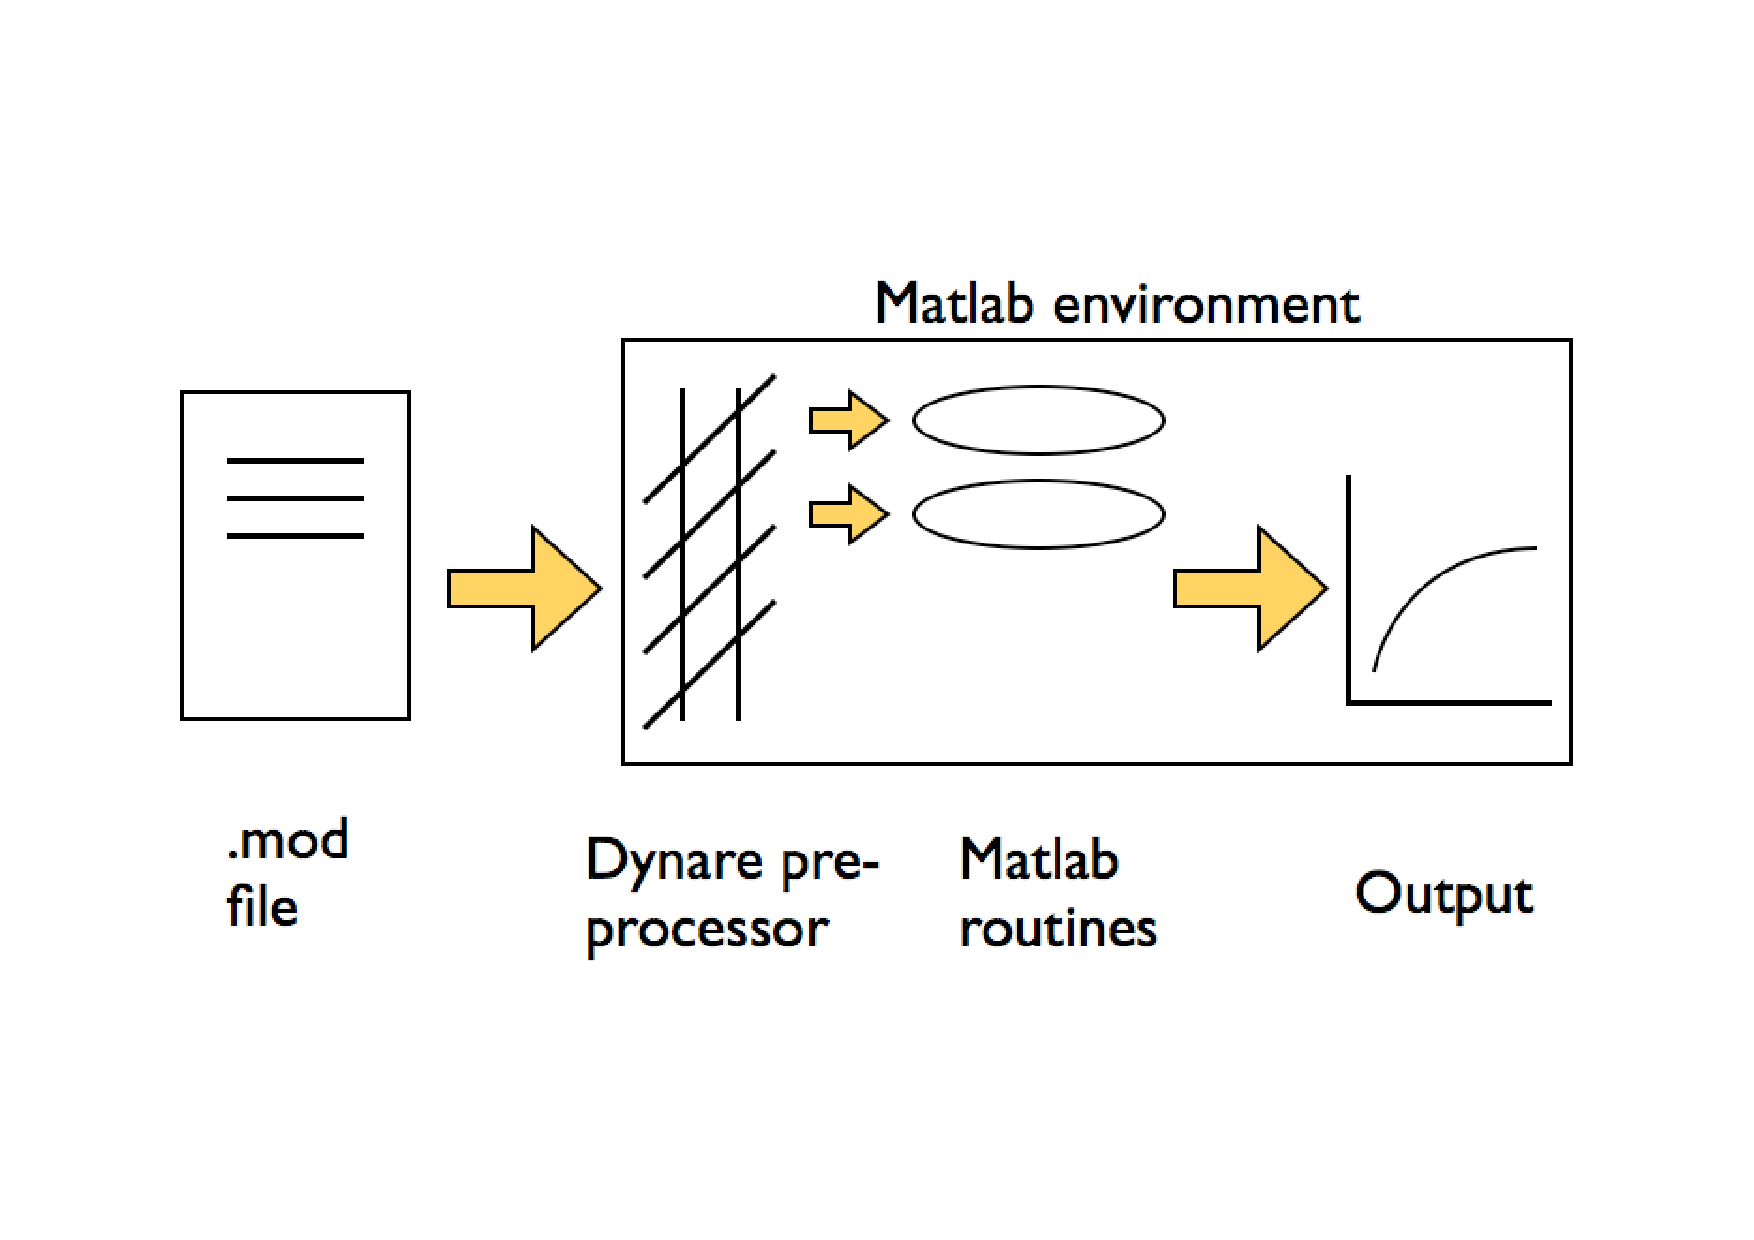
\includegraphics[width=1.0\textwidth]{P_DynareStruct2}
		\end{center}
		\caption[Dynare, a bird's eyeview]{The .mod file being read by the Dynare pre-processor, which then calls the relevant Matlab routines to carry out the desired operations and display the results.}
	\end{figure}
	
	Figure \ref{fig:dyn} gives you an overview of the way Dynare works. Basically, the model and its related attributes, like a shock structure for instance, is written equation by equation in an editor of your choice. The resulting file will be called the .mod file. That file is then called from Matlab. This initiates the Dynare pre-processor which translates the .mod file into a suitable input for the Matlab routines (more precisely, it creates intermediary Matlab or C files which are then used by Matlab code) used to either solve or estimate the model. Finally, results are presented in Matlab. Some more details on the internal files generated by Dynare is given in section \ref{sec:dynfiles} in chapter \ref{ch:soladv}. 
	
	Each of these steps will become clear as you read through the User Guide, but for now it may be helpful to summarize \textbf{what Dynare is able to do}:
	\begin{itemize}
		\item compute the steady state of a model
		\item compute the solution of deterministic models
		\item compute the first and second order approximation to solutions of stochastic models
		\item estimate parameters of DSGE models using either a maximum likelihood or a Bayesian approach
		\item compute optimal policies in linear-quadratic models
	\end{itemize}
	
	
	\section{Additional sources of help}
	While this User Guide tries to be as complete and thorough as possible, you will certainly want to browse other material for help, as you learn about new features, struggle with adapting examples to your own work, and yearn to ask that one question whose answer seems to exist no-where. At your disposal, you have the following additional sources of help:
	\begin{itemize}
		\item \href{http://www.dynare.org/documentation-and-support/manual}{\textbf{Reference Manual}}: this manual covers all Dynare commands, giving a clear definition and explanation of usage for each. The User Guide will often introduce you to a command in a rather loose manner (mainly through examples); so reading corresponding command descriptions in the Reference Manual is a good idea to cover all relevant details.
		\item \href{http://www.dynare.org/documentation-and-support/examples}{\textbf{Official online examples}}: the Dynare website includes other examples - usually well documented - of .mod files covering models and methodologies introduced in recent papers.
		\item \href{http://www.dynare.org/phpBB3}{\textbf{Dynare forums}}: this lively online discussion forum allows you to ask your questions openly and read threads from others who might have run into similar difficulties.
		\item \href{http://www.dynare.org/documentation-and-support/faq}{\textbf{Frequently Asked Questions}} (FAQ): this section of the Dynare site emphasizes a few of the most popular questions in the forums.
		\item \href{http://www.dsge.net}{\textbf{DSGE.net}}: this website, run my members of the Dynare team, is a resource for all scholars working in the field of DSGE modeling. Besides allowing you to stay up to date with the most recent papers and possibly make new contacts, it conveniently lists conferences, workshops and seminars that may be of interest.
	\end{itemize}
	
	\section{Nomenclature}
	To end this introduction and avoid confusion in what follows, it is worthwhile to agree on a few \textbf{definitions of terms}. Many of these are shared with the Reference Manual.
	\begin{itemize}
		\item \textbf{Integer} indicates an integer number.
		\item \textbf{Double} indicates a double precision number. The following syntaxes are valid: 1.1e3, 1.1E3, 1.1E-3, 1.1d3, 1.1D3
		\item \textbf{Expression} indicates a mathematical expression valid in the underlying language (e.g. Matlab).
		\item \textbf{Variable name} indicates a variable name. \textbf{\textsf{NOTE!}} These must start with an alphabetical character and can only contain other alphabetical characters and digits, as well as underscores (\_). All other characters, including accents, and \textbf{spaces}, are forbidden.
		\item \textbf{Parameter name} indicates a parameter name which must follow the same naming conventions as above.
		\item \textbf{Filename} indicates a file name valid in your operating system. Note that Matlab requires that names of files or functions start with alphabetical characters; this concerns your Dynare .mod files.
		\item \textbf{Command} is an instruction to Dynare or other program when specified.
		\item \textbf{Options} or optional arguments for a command are listed in square brackets \mbox{[ ]} unless otherwise noted. If, for instance, the option must be specified in parenthesis in Dynare, it will show up in the Guide as [(option)].
		\item \textbf{\texttt{Typewritten text}} indicates text as it should appear in Dynare code.
	\end{itemize}
	
	\section{v4.5, what's new and backward compatibility}
	The current version of Dynare - for which this guide is written - is version 4.5. With respect to version 4.4, this new version introduces several important features, as well as improvements, optimizations of routines and bug fixes. The major new features are the following:
	\begin{itemize}
		\item Ramsey policy
		
		
		Added command ramsey\_model that builds the expanded model with FOC conditions for the planner's problem but doesn't perform any computation. Useful to compute Ramsey policy in a perfect foresight model and for estimation,
		
		
		ramsey\_policy accepts multipliers in its variable list and displays results for them.
		
		\item Perfect foresight models
		
		
		New commands perfect\_foresight\_setup (for preparing the simulation) and perfect\_foresight\_solver (for computing it). The old simul command still exist and is now an alias for perfect\_foresight\_setup + perfect\_foresight\_solver. It is no longer possible to manipulate by hand the contents of
		oo\_.exo\_simul when using simul. People who want to do it must first call perfect\_foresight\_setup, then do the manipulations, then call perfect\_foresight\_solver,
		
		
		By default, the perfect foresight solver will try a homotopy method if it fails to converge at the first try. The old behavior can be restored with the no\_homotopy option,
		
		
		New option stack\_solve\_algo=7 that allows specifying a solve\_algo solver for solving the model,
		
		
		New option solve\_algo that allows specifying a solver for solving the model when using stack\_solve\_algo=7,
		
		
		New option lmmcp that solves the model via a Levenberg-Marquardt mixed complementarity problem (LMMCP) solver,
		
		
		New option robust\_lin\_solve that triggers the use of a robust linear solver for the default solve\_algo=4,
		
		
		New options tolf and tolx to control termination criteria of solvers,
		
		
		New option endogenous\_terminal\_period to simul,
		
		
		Added the possibility to set the initial condition of the (stochastic) extended path simulations with the histval block.
		
		\item Optimal simple rules
		
		
		Saves the optimal value of parameters to oo\_.osr.optim\_params,
		
		
		New block osr\_params\_bounds allows specifying bounds for the estimated parameters,
		
		
		New option opt\_algo allows selecting different optimizers while the new option optim allows specifying the optimizer options,
		
		
		The osr command now saves the names, bounds, and indices for the estimated parameters as well as the indices and weights of the variables entering the objective function into M\_.osr.
		
		\item Forecasts and Smoothing
		
		
		The smoother and forecasts take uncertainty about trends and means into account,
		
		
		Forecasts accounting for measurement error are now saved in fields of the form HPDinf\_ME and HPDsup\_ME,
		
		
		New fields oo\_.Smoother.Trend and oo\_.Smoother.Constant that save the trend and constant parts of the smoothed variables,
		
		
		new field oo\_.Smoother.TrendCoeffs that stores the trend coefficients.
		
		
		Rolling window forecasts allowed in estimation command by passing a vector to first\_obs,
		
		
		The calib\_smoother command now accepts the loglinear, prefilter, first\_obs and filter\_decomposition options.
		\item Estimation
		
		
		New options: logdata, consider\_all\_endogenous,consider\_only\_observed, posterior\_max\_subsample\_draws, mh\_conf\_sig, diffuse\_kalman\_tol, dirname, nodecomposition.
		
		
		load\_mh\_file and mh\_recover now try to load chain's proposal density\,
		
		
		New option load\_results\_after\_load\_mh that allows loading some posterior results from a previous run if no new MCMC draws areadded,
		
		
		New option posterior\_nograph that suppresses the generation of graphs associated with Bayesian IRFs, posterior smoothed objects, and posterior forecasts,
		
		
		Saves the posterior density at the mode in oo\_.posterior.optimization.log\_density,
		
		
		The filter\_covariance option now also works with posterior sampling like Metropolis-Hastings,
		
		
		New option no\_posterior\_kernel\_density to suppress computation of kernel density of posterior objects,
		
		
		Recursive estimation and forecasting now provides the individual
		oo\_ structures for each sample in oo\_recursive\_,
		
		
		The trace\_plot command can now plot the posterior density,
		
		
		New command generate\_trace\_plots allows generating all trace plots for one chain,
		
		
		New commands prior\_function and posterior\_function that execute a user-defined function on parameter draws from the prior/posterior distribution ,
		
		
		New option huge\_number for replacement of infinite bounds with large number during mode\_compute,
		
		
		New option posterior\_sampling\_method allows selecting the new posterior sampling options: tailored\_random\_block\_metropolis\_hastings (Tailored randomized block (TaRB) Metropolis-Hastings), slice (Slice sampler), independent\_metropolis\_hastings (Independent Metropolis-Hastings).
		
		
		New option posterior\_sampler\_options that allow controlling the options of the posterior\_sampling\_method; its scale\_file-option pair allows loading the \_mh\_scale.mat-file storing the tuned scale factor from a previous run of mode\_compute=6,
		
		
		New option raftery\_lewis\_diagnostics that computes Raftery/Lewis (1992) convergence diagnostics,
		
		
		New option fast\_kalman\_filter that provides fast Kalman filter using Chandrasekhar recursions as described in Ed Herbst (2015),
		
		
		The dsge\_var option now saves results at the posterior mode into oo\_.dsge\_var,
		
		
		New option smoothed\_state\_uncertainty to provide the uncertainty estimate for the smoothed state estimate from the Kalman smoother,
		
		
		New prior density: generalized Weibull distribution,
		
		
		Option mh\_recover now allows continuing a crashed chain at the last save mh-file,
		
		
		New option nonlinear\_filter\_initialization for the estimation command. Controls the initial covariance matrix of the state variables in nonlinear filters.
		
		
		The conditional\_variance\_decomposition option now displays output and stores it as a LaTeX-table when the TeX option is invoked,
		
		
		The use\_calibration to estimated\_params\_init now also works with ML,
		
		
		Improved initial estimation checks.
		
		
		
		
		\item Steady state
		
		
		The default solver for finding the steady state is now a trust-region solver (can be triggered explicitly with option
		solve\_algo=4),
		
		
		New options tolf and tolx to control termination criteria of solver,
		
		
		The debugging mode now provides the termination values in steady state finding.
		
		
		
		
		\item Stochastic simulations
		
		
		New options nodecomposition,
		
		
		New option bandpass\_filter to compute bandpass-filtered theoretical and simulated moments,
		
		
		New option one\_sided\_hp\_filter to compute one-sided HP-filtered simulated moments,
		
		
		stoch\_simul displays a simulated variance decomposition when simulated moments are requested,
		
		
		stoch\_simul saves skewness and kurtosis into respective fields of oo\_ when simulated moments have been requested,
		
		
		stoch\_simul saves the unconditional variance decomposition in oo\_.variance\_decomposition,
		
		
		New option dr\_display\_tol that governs omission of small terms in display of decision rules,
		
		
		The stoch\_simul command now prints the displayed tables as LaTeX code when the new TeX option is enabled,
		
		
		The loglinear option now works with lagged and leaded exogenous variables like news shocks,
		
		
		New option spectral\_density that allows displaying the spectral density of (filtered) endogenous variables,
		
		
		New option contemporaneous\_correlation that allows saving contemporaneous correlations in addition to the covariances.
		
		
		
		
		\item Identification
		
		
		New options diffuse\_filter and prior\_trunc,
		
		
		The identification command now supports correlations via simulated moments,
		
		
		
		
		\item Sensitivity analysis
		
		
		New blocks irf\_calibration and moment\_calibration,
		
		
		Outputs LaTeX tables if the new TeX option is used,
		
		
		New option relative\_irf to irf\_calibration block.
		
		
		
		
		\item Conditional forecast
		
		Command conditional\_forecast now takes into account histval block if present.
		
		
		
		\item Shock decomposition
		
		
		New option colormap to shocks\_decomposition for controlling the color map used in the shocks decomposition graphs,
		
		
		shocks\_decomposition now accepts the nograph option,
		
		
		New command realtime\_shock\_decomposition that for each period T= [presample,...,nobs] allows computing the:
		
		
		realtime historical shock decomposition Y(t|T), i.e. without observing data in [T+1,...,nobs]
		
		
		forecast shock decomposition Y(T+k|T)
		
		
		realtime conditional shock decomposition Y(T+k|T+k)-Y(T+k|T)
		
		
		
		
       New block shock\_groups that allows grouping shocks for the shock\_decomposition and realtime\_shock\_decomposition commands.
		
		
		New command plot\_shock\_decomposition that allows plotting the results from shock\_decomposition and realtime\_shock\_decomposition for different vintages and shock groupings.
		
		
		
		
		\item Macroprocessor
		
		
		Can now pass a macro-variable to the \@\#include macro directive,
		
		
		New preprocessor flag -I, macro directive \@\#includepath, and dynare config file block [paths] to pass a search path to the macroprocessor to be used for file inclusion via \@\#include.
		
		
		
		
		\item Command line
		
		
		New option onlyclearglobals (do not clear JIT compiled functions with recent versions of Matlab),
		
		
		New option minimal\_workspace to use fewer variables in the current workspace,
		
		
		New option params\_derivs\_order allows limiting the order of the derivatives with respect to the parameters that are calculated by the preprocessor,
		
		
		New command line option mingw to support the MinGW-w64 C/C++ Compiler from TDM-GCC for use\_dll.
		
		
		
		
		\item dates/dseries/reporting classes
		
		
		New methods abs, cumprod and chain,
		
		
		New option tableRowIndent to addTable,
		
		
		Reporting system revamped and made more efficient, dependency on matlab2tikz has been dropped.
		
		
		
		
		\item Optimization algorithms
		
		
		mode\_compute=2 Uses the simulated annealing as described by Corana et al. (1987),
		
		
		mode\_compute=101 Uses SOLVEOPT as described by Kuntsevich and Kappel (1997),
		
		
		mode\_compute=102 Uses simulannealbnd from Matlab's Global Optimization Toolbox (if available),
		
		
		New option silent\_optimizer to shut off output from mode computing/optimization,
		
		
		New options verbosity and SaveFiles to control output and saving of files during mode computing/optimization.
		
		
		
		
		\item LaTeX output
		
		
		New command write\_latex\_original\_model,
		
		
		New option write\_equation\_tags to write\_latex\_dynamic\_model that allows printing the specified equation tags to the generate
		LaTeX code,
		
		
		New command write\_latex\_parameter\_table that writes the names and values of model parameters to a LaTeX table,
		
		
		New command write\_latex\_prior\_table that writes the descriptive statistics about the prior distribution to a LaTeX table,
		
		
		New command collect\_latex\_files that creates one compilable LaTeX file containing all TeX-output.
		
		
		
		
		\item Misc.
		
		
		Provides 64bit preprocessor,
		
		
		Introduces new path management to avoid conflicts with other toolboxes,
		
		
		Full compatibility with Matlab 2014b's new graphic interface,
		
		
		When using model(linear), Dynare automatically checks whether the model is truly linear,
		
		
		usedll: the msvc option now supports normcdf, acosh, asinh, and atanh,
		
		
		New parallel option NumberOfThreadsPerJob for Windows nodes that sets the number of threads assigned to each remote MATLAB/Octave run,
		
		
		Improved numerical performance of schur\_statespace\_transformation for very large models,
		
		
		The all\_values\_required option now also works with histval,
		
		
		Add missing horizon option to ms\_forecast,
		
		
		BVAR now saves the marginal data density in oo\_.bvar.log\_marginal\_data\_density and stores prior and posterior information in oo\_.bvar.prior and oo\_.bvar.posterior.
	\end{itemize}
	
	
	
	
	\chapter{Installing Dynare}
	
	\section{Dynare versions}
	
	Dynare runs on both \href{http://www.mathworks.com/products/matlab/}{\textbf{MATLAB}} and \href{http://www.octave.org}{\textbf{GNU Octave}}.
	
	There used to be versions of Dynare for \textbf{Scilab} and \textbf{Gauss}. Development of the Scilab version stopped after Dynare version 3.02 and that for Gauss after Dynare version 1.2.
	
	This User Guide will exclusively \textbf{focus on Dynare version 4.0 and later}.
	
	You may also be interested by another program, \textbf{Dynare++}, which is a standalone C++ program specialized in computing k-order approximations of dynamic stochastic general equilibrium models. Note that Dynare++ is distributed along with Dynare since version 4.1. See the \href{http://www.dynare.org/documentation-and-support/dynarepp}{Dynare++ webpage} for more information. 
	
	\section{System requirements}
	Dynare can run on Microsoft Windows, as well as Unix-like operating systems, in particular GNU/Linux and Mac OS X. If you have questions about the support of a particular platform, please ask your question on \href{http://www.dynare.org/phpBB3}{\textbf{Dynare forums}}.
	
	To run Dynare, it is recommended to allocate at least 256MB of RAM to the platform running Dynare, although 512MB is preferred. Depending on the type of computations required, like the very processor intensive Metropolis Hastings algorithm, you may need up to 1GB of RAM to obtain acceptable computational times.
	
	\section{Installing Dynare}
	
	Please refer to the section entitled ``Installation and configuration'' in the \href{http://www.dynare.org/documentation-and-support/manual}{Dynare reference manual}.
	
	\section{MATLAB particularities}
	
	A question often comes up: what special MATLAB toolboxes are necessary to run Dynare? In fact, no additional toolbox is necessary for running most of Dynare, except maybe for optimal simple rules (see chapter \ref{ch:ramsey}), but even then remedies exist (see the \href{http://www.dynare.org/phpBB3}{Dynare forums} for discussions on this, or to ask your particular question). But if you do have the `optimization toolbox' installed, you will have additional options for solving for the steady state (solve\_algo option) and for searching for the posterior mode (mode\_compute option), both of which are defined later. 
	
	\chapter{Solving Steady State - basics}
	Basically, you have to remove all the time indices (t-1,t,t+1,...) on the endogenous and exogenous variables in all the equations, and express the endogenous variables as functions of the exogenous variables and parameters. This cannot be done analytically in all models, and often you will have to resort on a numerical solver to obtain the steady state (for given values of the parameters and exogenous variables). This is what Dynare does if you do not provide a closed form expression for the steady state. In small models (basic RBC or NK models), it is possible to obtain an analytical expression for the steady state.
	
	As is known to all, the steady-state value of the DSGE model is very difficult to solve, especially for complex nonlinear models. When we use the DSGE model, usually more than $80\%$ of the time may be spent on solving the steady-state values of endogenous variables. Doing so borders on a form of art, and luck is unfortunately part of the equation. Therefore, the following methods/skills/steps may be of some help to you.
	
	
	\section{Analytical Solutions} \label{sec:distcn}
	
	First of all, let's look at a simple model.

	The equilibrium system of the model is:
	
	\begin{equation}\label{label}
		C_t^{\sigma}\theta N_t^{\phi}=w_t
	\end{equation}
	
	\begin{equation}\label{label}
		E_t\frac{C_{t+1}^{\sigma}}{C_t^{\sigma}}=\beta E_t(R_{t+1}+(1-\delta))
	\end{equation}
	
	\begin{equation}\label{label}
		E_t\frac{C_{t+1}^{\sigma}}{C_t^{\sigma}}=\beta E_t(1+r_t)
	\end{equation}
	
	\begin{equation}\label{label}
		K_{t+1}=I_t+(1-\delta)K_t
	\end{equation}
	
	\begin{equation}\label{label}
		\alpha A_tK_t^{\alpha-1}N_t^{1-\alpha}=R_t
	\end{equation}
	
	\begin{equation}\label{label}
		(1-\alpha)A_tK_t^{\alpha}N_t^{-\alpha}=w_t
	\end{equation}
	
	\begin{equation}\label{label}
		Y_t=A_tK_t^{\alpha}N_t^{1-\alpha}
	\end{equation}
	
	\begin{equation}\label{label}
		Y_t=C_t+I_t
	\end{equation}
	
	\begin{equation}\label{label}
		lnA_t=\rho lnA_{t-1}+\epsilon_t
	\end{equation}
	
	(3.1) is the labor supply equation. (3.2) is the investment-saving equilibrium, which is the capital Euler equation. (3.3) is also the investment-saving equilibrium, which is the bond Euler equation. (3.4) is the capital accumulation equation. (3.5) is the capital demand equation. (3.6) is the labor demand equation. (3.7) is the production function. (3.8) It is the product market clearing. (3.9) is the productivity shock. Among them, there is a lead variable $C_{t+1}$, and two state variables $K_t,A_t$. The model equilibrium system contains 9 endogenous variables $Y_t,C_t,N_t,K_t,I_t,w_t,R_t,r_t,A_t$, and 9 equations.
	
	
	The equilibrium of the model has been defined above, and then we will define and solve the steady state of the model. Steady state means that the endogenous variables are equal in each period,$E_tx_{t+1}=x_t=x_{t-1}=x_{ss}$.
	
	First, in the steady state, remove the time subscripts of all variables. $E_t\epsilon_t=0$, therefore, $A=1$ can be obtained from the productivity evolution equation (3.9). And in the steady state, $K_{t+1}=K_t=K,C_{t+1}=C_t=C$.
	
	Starting from Euler's equations (3.2) and (3.3), it is easiest to solve the steady state. 
	
	(1) From (3.2) and (3.3),
	
	\begin{equation}\label{label}
		\begin{split}
			\beta(R+1-\delta)=1\\
			\Leftrightarrow R=\frac{1}{\beta}+\delta-1
		\end{split}
	\end{equation}
	
	\begin{equation}\label{label}
		\begin{split}
			\beta(1+r)=1\\
			\Leftrightarrow r=\frac{1}{\beta}-1
		\end{split}
	\end{equation}
	
	(2) From the capital demand function (3.5), the steady state of the capital-labor ratio can be solved:
	
	\begin{equation}\label{label}
		\begin{split}
			R=\alpha(\frac{K}{N})^{\alpha-1}\\
			\Leftrightarrow \frac{K}{N}=(\frac{R}{\alpha})^{\frac{1}{\alpha-1}}\\
			\Leftrightarrow \frac{K}{N}=(\frac{\alpha}{\frac{1}{\beta}+\delta-1})^{\frac{1}{1-\alpha}}
		\end{split}
	\end{equation}
	
	Note that the third line of (3.12) is obtained by substituting the result of (3.10) into the second line.
	
	(3)Substituting the capital-labor steady-state ratio of (3.12) into the labor demand equation of (3.6), we get
	
	\begin{equation}\label{label}
		\begin{split}
			w=(1-\alpha)(\frac{K}{N})^{\alpha}\\
			\Leftrightarrow w=(1-\alpha)(\frac{\alpha}{\frac{1}{\beta}+\delta-1})^{\frac{\alpha}{1-\alpha}}
		\end{split}
	\end{equation}
	
	(4)From the capital accumulation equation (3.4), we can get $I=\delta K$, and from the production function (3.7), we can get $Y=(\frac{K}{N})^{\alpha}N$.
	
	(5)Substituting the two formulas in the fourth step into the product market clearing equation (3.8) to obtain
	
	\begin{equation}\label{label}
		\begin{split}
			(\frac{K}{N})^{\alpha}N=C+\delta K\\
			\Leftrightarrow \frac{C}{N}=(\frac{K}{N})^{\alpha}-\delta \frac{K}{N}
		\end{split}
	\end{equation}
	
	(6)Combining the above equation (3.14) with the labor demand equation (3.13) , and $\frac{K}{N},w$ is known, thus
	
	\begin{equation}\label{label}
		\left\{
		\begin{aligned}
			C^{\sigma}\theta N_t^{\phi}=w\\
			\frac{C}{N}=(\frac{K}{N})^{\alpha}-\delta \frac{K}{N}\\
		\end{aligned}
		\right.
	\end{equation}
	
	Through the above equation (3.15), the steady-state value of consumption and labor $C,N$ can be solved. Once the steady state of labor $N$ is obtained, it can be substituted into the steady state of capital-labor ratio (3.12) to solve the steady state of capital $K$, and then the steady state of output and investment $Y,I$ can be obtained.
	
	For small scale DSGE models, we can find analytical solutions for each endogenous variable. Therefore, the accurate steady-state values can be obtained. However, because Dynare is more sensitive to the initial values, it may still report an error at this time. So we need to add some optimization options after the steady command:
	
	\begin{itemize}
		\item $solve\_algo=0:$ Use the fsolve function in the Optimization Toolbox in Matlab.
		\item $solve\_algo=1:$ Use the Dynare built-in nonlinear equation algorithm.
		\item $solve\_algo=2:$ Divide the model into recursive modules and solve each module one by one.
		\item $solve\_algo=3:$ Use the Sims algorithm. This is the default option.
	\end{itemize}
	
	\section{Adding new variable one by one}
	
	Analytical methods are generally applicable to small-scale DSGE models.  However, the analytical solutions are difficult to be solved for medium and large scale models. Fortunately, the DSGE model is very modular, and the complex models are basically extended based on the baseline model (small scale). Therefore, we can gradually introduce the sectors or factors we are interested in to expand to new models. For example, in the RBC model, the monopolistic competition structure of enterprises is introduced first, and then the price stickiness of intermediate product enterprises is introduced, thus forming the New Keynesian model.

        This idea of adding factors step by step also provides an idea for us to solve the steady state. That is to say, when we solve the steady state, we also follow the path of $baseline model - extended model 1 - extended model 2 - \cdots - final model $.

        For example, in the RBC model of the previous section, we introduced the monopolistic competition factor, then the equilibrium system becomes:
	
	\begin{equation}\label{label}
		C_t^{\sigma}\theta N_t^{\phi}=w_t
	\end{equation}
	
	\begin{equation}\label{label}
		E_t\frac{C_{t+1}^{\sigma}}{C_t^{\sigma}}=\beta E_t(R_{t+1}+(1-\delta))
	\end{equation}
	
	\begin{equation}\label{label}
		E_t\frac{C_{t+1}^{\sigma}}{C_t^{\sigma}}=\beta E_t(1+r_t)
	\end{equation}
	
	\begin{equation}\label{label}
		K_{t+1}=I_t+(1-\delta)K_t
	\end{equation}
	
	\begin{equation}\label{label}
		\alpha MC_t A_tK_t^{\alpha-1}N_t^{1-\alpha}=R_t
	\end{equation}
	
	\begin{equation}\label{label}
		(1-\alpha)MC_t A_tK_t^{\alpha}N_t^{-\alpha}=w_t
	\end{equation}
	
	\begin{equation}\label{label}
		Y_t=A_tK_t^{\alpha}N_t^{1-\alpha}
	\end{equation}
	
	\begin{equation}\label{label}
		Y_t=C_t+I_t
	\end{equation}
	
	\begin{equation}\label{label}
		MC_t=\frac{\xi_t-1}{\xi_t}
	\end{equation}
	
	\begin{equation}\label{label}
		lnA_t=\rho lnA_{t-1}+\epsilon_t
	\end{equation}
	
	\begin{equation}\label{label}
		ln\xi _t=(1-\rho_{\xi})ln\xi+\rho_{\xi} ln\xi_{t-1}+\epsilon_{\xi}
	\end{equation}
	
	The equilibrium system includes 10 endogenous variables $Y_t,C_t,N_t,K_t,I_t,w_t,R_t,r_t,MC_t,A_t,\xi_t$, and 10 equations.
	
	
	\textbf{Steady State}
	
The equilibrium of the model has been defined above, and in the following we will define and solve the steady state of the model. Steady state means that the endogenous variables are equal in each period, $E_tx_{t+1}=x_t=x_{t-1}=x_{ss}$. Firstly, at steady state, the time subscripts of all variables are removed. $E_t\epsilon_t=0$. Therefore, $A=1$ can be obtained from the productivity evolution equation (3.25). In additional, at the steady state, $K_{t+1}=K_t=K, C_{t+1}=C_t=C$.

The steady state is easiest to be solved by starting with Euler's equations (3.17) and (3.18).

(1) ~ From (3.17) and (3.18), we can get that
	
	\begin{equation}\label{label}
		\begin{split}
			\beta(R+1-\delta)=1\\
			\Leftrightarrow R=\frac{1}{\beta}+\delta-1
		\end{split}
	\end{equation}
	
	\begin{equation}\label{label}
		\begin{split}
			\beta(1+r)=1\\
			\Leftrightarrow r=\frac{1}{\beta}-1
		\end{split}
	\end{equation}
	
	(2)~The steady state of the capital-labor ratio can be solved from the capital demand function (3.20):
	
	\begin{equation}\label{label}
		\begin{split}
			R=\alpha MC(\frac{K}{N})^{\alpha-1}\\
			\Leftrightarrow \frac{K}{N}=(\frac{R}{\alpha MC})^{\frac{1}{\alpha-1}}\\
			\Leftrightarrow \frac{K}{N}=(\frac{\alpha MC}{\frac{1}{\beta}+\delta-1})^{\frac{1}{1-\alpha}}
		\end{split}
	\end{equation}
	
	Note that the third line of (3.27) is obtained by substituting the result of (3.25) into the second line.
	
	(3)~According to the capital-labor steady-state ratio of (3.27), substituting it into the labor demand equation of (3.21), we get:
	
	\begin{equation}\label{label}
		\begin{split}
			w=(1-\alpha)(\frac{K}{N})^{\alpha}\\
			\Leftrightarrow w=(1-\alpha)(\frac{\alpha MC}{\frac{1}{\beta}+\delta-1})^{\frac{\alpha}{1-\alpha}}
		\end{split}
	\end{equation}
	
	(4)~From the capital accumulation equation (3.19), we know that $I=\delta K$, and from the production function (3.22), we know that $Y=(\frac{K}{N})^{\alpha}N$.
	
	(5)~Substituting the two equations in the fourth step into the product market clearing equation (3.23), we get
	
	\begin{equation}\label{label}
		\begin{split}
			(\frac{K}{N})^{\alpha}N=C+\delta K\\
			\Leftrightarrow \frac{C}{N}=(\frac{K}{N})^{\alpha}-\delta \frac{K}{N}
		\end{split}
	\end{equation}
	
	(6)~Combining the above equation (3.29) with the labor demand equation (3.16), and $\frac{K}{N},w$ is known, we get
	
	\begin{equation}\label{label}
		\left\{
		\begin{aligned}
			C^{\sigma}\theta N_t^{\phi}=w\\
			\frac{C}{N}=(\frac{K}{N})^{\alpha}-\delta \frac{K}{N}\\
		\end{aligned}
		\right.
	\end{equation}
	
	The steady state value of consumption and labor $C,N$ can be solved by the above equation (3.29). Once the steady state of labor $N$ is obtained, it can be substituted into the capital-labor ratio steady state (3.27) to solve the capital steady state $K$, and then obtain the output and investment steady state $Y,I$.
	
	(7)~The marginal cost steady state MC can be solved by the price mark-up shocks (3.26) and (3.24).
	

     For another example, we introduce the price stickiness factor in the above extended model. Then we can get the following equilibrium system:
	
	\begin{equation}\label{label}
		C_t^{\sigma}\theta N_t^{\phi}=w_t
	\end{equation}
	
	\begin{equation}\label{label}
		E_t\frac{C_{t+1}^{\sigma}}{C_t^{\sigma}}=\beta E_t(R_{t+1}+(1-\delta))
	\end{equation}
	
	\begin{equation}\label{label}
		E_t\frac{C_{t+1}^{\sigma}}{C_t^{\sigma}}=\beta E_t(1+r_t)
	\end{equation}
	
	\begin{equation}\label{label}
		K_{t+1}=I_t+(1-\delta)K_t
	\end{equation}
	
	\begin{equation}\label{label}
		\frac{\alpha}{1-\alpha} \frac{N_t}{K_t}=\frac{R_t}{w_t}
	\end{equation}
	
	\begin{equation}\label{label}
		Y_tv_t^p=A_tK_t^{\alpha}N_t^{1-\alpha}
	\end{equation}
	
	\begin{equation}\label{label}
		Y_t=C_t+I_t
	\end{equation}
	
	\begin{equation}\label{label}
		MC_t=\frac{w_t}{(1-\alpha)A_t(\frac{K_t}{N_t})^{\alpha}}\frac{\xi-1}{\xi}
	\end{equation}
	
	\begin{equation}\label{label}
		lnA_t=\rho lnA_{t-1}+\epsilon_t
	\end{equation}
	
	\begin{equation}\label{label}
		v_t^p=(1-\phi)(1+\pi_t^{\star})^{-\xi}(1+\pi_t)^{\xi}+(1+\pi_t)^{\xi}\phi v_{t-1}^p
	\end{equation}
	
	\begin{equation}\label{label}
		(1+\pi_t)^{1-\xi}=(1-\phi)(1+\pi_t^{\star})^{1-\xi}+\phi
	\end{equation}
	
	\begin{equation}\label{label}
		1+\pi_t^{\star}=\frac{\xi}{\xi-1}(1+\pi_t)\frac{x_{1t}}{x_{2t}}
	\end{equation}
	
	\begin{equation}\label{label}
		x_{1t}=C_t^{-\sigma}MC_tY_t+\phi \beta E_t(1+\pi_{t+1})^{\xi}x_{1,t+1}
	\end{equation}
	
	\begin{equation}\label{label}
		x_{2t}=C_t^{-\sigma}Y_t+\phi \beta E_t(1+\pi_{t+1})^{\xi-1}x_{2,t+1}
	\end{equation}
	
	\begin{equation}\label{label}
		r_t=(1-\rho_r)r+\rho_rr_{t-1}+(1-\rho_r)(\phi_{\pi}(\pi_t-\pi)+\phi_y(lnY_t-lnY))+\epsilon_t
	\end{equation}
	
	The equilibrium system includes 15 endogenous variables $Y_t,C_t,N_t,K_t,I_t,w_t,R_t,r_t,MC_t,A_t,v_t^p,\pi_t,\pi_t^{\star},x_{1t},x_{2t}$, and 15 equations.

	
	\textbf{Steady State}
	
	First, we can solve $\pi$ from (3.47);
	Then, we substitute $\pi$ into (3.43), and solve $\pi^{\star}$;
	
	From(3.45) and (3.46), we can get
	$$MC=\frac{x_{1}}{x_{2}}\frac{1-\phi \beta(1+\pi)^{\xi}}{1-\phi \beta(1+\pi)^{\xi-1}}$$
	
	Once we know the steady state of MC, we can go back to (3.29) to solve the steady state of $\frac{K}{N}$, and then solve the steady state values of other endogenous variables in turn.
	
	Exercise: The model that introducing fiscal policy.
	
	
	\section{Calibrating Steady State}
	
	Calibrating steady state? We seem to have only heard of calibrating parameters. In fact, both are the same.
	
	Parameter calibration seems to be the most ‘despised’ but must-use method. However, what I want to say is that this method was used by the ancestors of econometrics when the Econometric Society was founded, and it is the cornerstone of all subsequent estimation methods.
	
	Kydland and Prescott (1982) used a method to convert the DSGE model they analyzed into an empirical analysis. The method they use is a calibration exercise. DeJong and Dave (2007) call this approach the basis of MM/ML/BL.
	
	We know that under the criticism of Lucas (1976) and Sims (1980), the estimation and hypothesis testing of probabilistic methods are not applicable to structural models. Therefore, the goal of the calibration exercise is to explore some specific quantitative problem with a parametric structural model. Kydland and Prescott (1991,, SJE; 1996, JEP) trace the historical origins of calibration linkages as an empirical research method, which you can read. Paragraph one of the constitution elaborated upon the motto by stating that the object of the Society should be to.promote studies that aim at a unification of the theoretical-quantitative and the empirical-quantitative approach to economic problems and that are penetrated by constructive and rigorous thinking similar to that which has come to dominate in the natural sciences. Any activitywhich promises ultimately to further such unification of theoretical and factual studies in economicshall be within the sphere of interest of the Society. ()Frisch(1933a))
	
	Moreover, Frisch (1933b) also used microdata to calibrate production technical parameters and to study the propagation mechanism of business cycle shocks. We all acknowledge that this approach has some flaws, especially with regard to model misspecification. However, as Prescott (1986) points out:
	‘The models constructed within this theoretical framework are necessarily highly abstract. Consequently, they are necessarily false, and statistical hypothesis testing will reject them. This does not imply, however, that nothing can be Learned from such quantitative theoretical exercises. I think much has already been learned and confidently predict that much more will be learned as other features of the environment are introduced. Prime candidates for study are the effects of public finance elements, a foreign sector, and, of course, monetary factors. The researchI review here is best viewed as a very promising beginning of a much larger research program.’
	
	In conclusion, calibration exercises are certainly an empirical tool (DeJong and Dave, 2007). Kydland and Prescott (1996, JEP) stated: ’It is important to note that calibration is not intended to obtain the magnitude of certain parameters, i.e. it is not an estimate.‘ \textcolor{red}{Therefore, when calibrating DSGE parameters, it usually comes from two aspects: one is the long-term mean; the other is the empirical results of micro-evidence. (For example, Cooley and Prescott (1995) used the microscopic evidence of Ghez and Becker (1975) to calibrate the parameters)}.
	
	The latter method, which we often use, is generally found in previous research results. However, after the financial crisis, more and more scholars use micro-data/micro-econometric models to estimate relevant parameters of key characteristics in their articles.
	
	The steady state is a mapping between endogenous variables and the parameters of the model. To calibrate a model, we somehow revert this mapping, expressing parameters as function of steady state ratios. For instance, in the Solow model, we have the law of motion for the physical capital stock:
	
	$$K_{t+1}=(1-\delta)K_t+I_t$$
	
	at the steady state we must have:
	
	$$K^{\star}=(1-\delta)K^{\star}+I^{\star}$$
	
	$$\delta K^{\star}=I^{\star}$$
	
	hence we know that the depreciation rate must be such that:
	
	$$\delta=\frac{I^{\star}}{K^{\star}}$$
	
	If we have long time series on physical capital and investment we can then calibrate the depreciation rate with average of the investment/capital ratio. Not all the parameters can be deduced from steady state considerations, since not all parameters will affect the steady state (rigidity parameters for instance). In this case we will have to consider other moments to calibrate these parameters.
	
	Next, let's take a look at how to use the long-term mean/data moment to obtain the steady-state value of the model endogenous variable.
	
	For example, Introduction to Modeling and Programming for DSGE (41): Financial Intermediation
	
	The steady state system is as follows:
	
	\begin{equation}\label{label}
		\frac{1}{c_t}=\frac{\gamma}{d_t}+\beta E_t\frac{1+r_t^d}{c_{t+1}}
	\end{equation}
	
	\begin{equation}\label{label}
		h_tl_t^{\phi}=\frac{w_t}{c_t}
	\end{equation}
	
	\begin{equation}\label{label}
		y_t=a_tk_{t-1}^{\alpha}l_t^{1-\alpha}
	\end{equation}
	
	\begin{equation}\label{label}
		r_t^k=\alpha a_tk_{t-1}^{\alpha-1}l_t^{1-\alpha}
	\end{equation}
	
	\begin{equation}\label{label}
		w_t=(1-\alpha)a_tk_{t-1}^{\alpha}l_t^{-\alpha}
	\end{equation}
	
	\begin{equation}\label{label}
		k_t=m_t^c+m_t^s
	\end{equation}
	
	\begin{equation}\label{label}
		m_t^s=(1-\kappa)ABS_t
	\end{equation}
	
	\begin{equation}\label{label}
		(1-\kappa)E_t(1+r_{t+1}^k-\delta)=1+r_t^a
	\end{equation}
	
	\begin{equation}\label{label}
		m_t^c+ABS_t=d_t+n_t
	\end{equation}
	
	\begin{equation}\label{label}
		n_t=\hat{\omega}m_t^c
	\end{equation}
	
	\begin{equation}\label{label}
		\omega_t=\hat{\omega}^{1-\rho_{\omega}}\omega_{t-1}^{\rho_{\omega}}\left(\frac{i_t/i_{t-1}}{gdp_t/gpd_{t-1}}\right)^{\Phi(1-\rho_{\omega})}e^{\epsilon_{\omega,t}}
	\end{equation}
	
	\begin{equation}\label{label}
		C(g_t)=-p_1ln(1+p_2g_t)
	\end{equation}
	
	\begin{equation}\label{label}
		F(\frac{ABS_t}{m_t^c})=\frac{\phi}{2}\left(\frac{ABS_t}{m_t^c}-\frac{ABS}{m^c}\right)^2
	\end{equation}
	
	\begin{equation}\label{label}
		1+C^{'}=\beta E_t\frac{c_t}{c_{t+1}}(1+r_t^d)
	\end{equation}
	
	\begin{equation}\label{label}
		(1+s_t)+(1-\omega_t)C^{'}-F^{'}\frac{ABS_t}{(m_t^c)^2}=\beta E_t\frac{c_t}{c_{t+1}}(1+r_{t+1}^k-\delta)
	\end{equation}
	
	\begin{equation}\label{label}
		1+C^{'}+F^{'}\frac{1}{m_t^c}=\beta E_t\frac{c_t}{c_{t+1}}(1-P_{t+1})(1+r_t^a)
	\end{equation}
	
	\begin{equation}\label{label}
		s_t=\rho_ss_{t-1}+\epsilon_{s,t}
	\end{equation}
	
	\begin{equation}\label{label}
		P_t=\rho_pP_{t-1}+\epsilon_{p,t}
	\end{equation}
	
	\begin{equation}\label{label}
		lna_t=\rho_alna_{t-1}+\epsilon_{a,t}
	\end{equation}
	
	\begin{equation}\label{label}
		lnh_t=(1-\rho_h)h+\rho_hh_{t-1}+\epsilon_{h,t}
	\end{equation}
	
	\begin{equation}\label{label}
		y_t=c_t+i_t+C(g_t)+F(\frac{ABS_t}{m_t^c})+s_tm_t^c+\kappa ABS_t
	\end{equation}
	
	\begin{equation}\label{label}
		gdp_t=c_t+i_t
	\end{equation}
	
	\begin{equation}\label{label}
		share_t=\frac{m_t^s}{k_t}
	\end{equation}
	
	\begin{equation}\label{label}
		leverage_t=\frac{m_t^c+ABS_t}{n_t}
	\end{equation}
	
	The macroeconomic indicators used include nominal GDP, GDP deflator, nominal net exports, nominal total consumption, CPI, employment, total shadow banking loans, total social financing, treasury bond repurchase rate, labor income share, fixed asset investment, Commercial bank capital adequacy ratio, etc. All are quarterly data.
	
	The macroeconomic indicators used include nominal GDP, GDP deflator, nominal net exports, nominal total consumption, CPI, employment, total shadow banking loans, total social financing, treasury bond repurchase rate, labor income share, fixed asset investment, Commercial bank capital adequacy ratio, etc. All are quarterly data.
	
	The period of labor income share data is Q1 1996 - Q4 2017. The period of fixed asset investment data is Q1 1992- Q4 2017. The period of GDP deflator, nominal net exports, nominal total consumption, CPI, employment, total shadow banking loans, and total social financing is Q1 2002 -Q4 2017. The above data are all from the Chinese macroeconomic database from Chang et al. (2015), Higgins and Tao Zha (2016). The period of nominal GDP is Q1 1992 - Q4 2017, and the data comes from the database of the National Bureau of Statistics of China. The period of the treasury bond repurchase rate is Q1 2000 - Q4 2017, and the data comes from the China Economic Database. The period of the capital adequacy ratio of commercial banks is Q1 2009 - Q4 2017. The data comes from the website of the China Banking Regulatory Commission.
	
	In the above data, the nominal value is all deflated by the relevant price index to obtain the actual value. Since the model economy in this paper does not include the foreign sector, net exports are deducted from GDP to obtain the GDP observations used in this paper. The shadow banking share observations used in this paper are obtained by dividing total shadow banking loans by total social financing. In addition to GDP observations and shadow banking shares, real consumption, employment, and Treasury repurchase rates are used for Bayesian estimation of some parameters of the model. Among them, GDP, consumption, employment, and shadow banking share are all processed by seasonal adjustment, logarithmic difference and mean removal processing, and the treasury bond repurchase rate is seasonally adjusted and mean removal.
	
	Data on other macroeconomic variables are used to calibrate model parameters.

	
	\begin{figure}[htbp!]
		\centering
		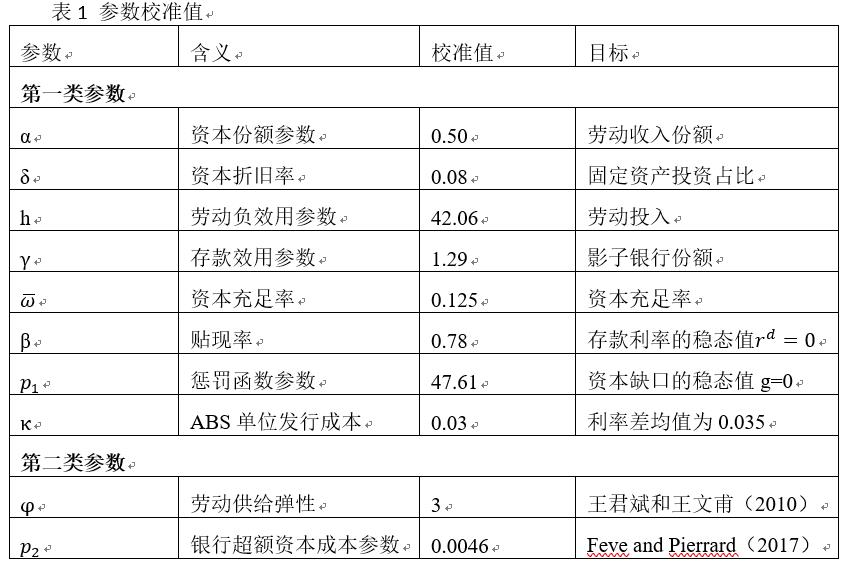
\includegraphics[width=0.8\linewidth]{FIG/table1}
		\centering
	\end{figure}
	
	
	\section{The External Files of Solving Steady State}
	
	Refer to DSGE Modeling and Programming: Medium-scale DSGE and its code
	
	
	\chapter{Occasionally Binding Constraints}
	
After the 2008 financial crisis, central banks around the world lowered interest rates to resist the economic downturn, which also brought nominal interest rates down/close to the zero lower bound in various countries. At the same time, households, firms, and financial institutions are also constrained by their own financing constraints due to falling asset prices. And ZLB and financing constraints are the most famous examples of OBCs.

Occasionally binding constraints are part of the economic landscape: for instance recent experience with the global financial crisis has highlighted the gravity of the lower bound constraint on interest rates; emerging economies have been affected by sudden stops, or slowdowns in private capital inflows, that occur from time to time; mortgagors are subject
to more stringent borrowing conditions when credit growth has been excessive or there is a downturn in the economy; workers have an aversion to taking pay cuts, a problem that is more acute during economic downturns.

The problem of modelling occasionally binding constraints is not a new one. The RBC and DSGE literatures have addressed these problems using a range of different methodologies. These include: eternally binding constraints, smooth approximation of occasionally binding constraints, the extended path algorithm, piecewise linear methods, anticipated shocks, global solution methods, and regime-switching methods.

\section{OBCs in Macroeconomics} \label{sec:modsetup}

OBCs imply that the model is nonlinear in nature, and thus, it also brings computational challenges for DSGE simulation and estimation. I have explained the characteristics of OBCs in DSGE many times in past tweets, such as DSGE Modeling and Programming Introduction (44): ZLB and News Shocks, [Add Dynare code] ZLB+OBC (Occasionally Binding Constraints), DSGE Modeling Getting Started with Programming (36): Financial Friction (3) et al.

One of the simplest and most straightforward approaches to handling occasionally binding constraints is to assume that the constraint is binding at all times. Following Brzoza-Brzezina et al. (2015), we refer to this approach as eternally binding constraints (EBC). Eternally binding constraints are commonly used in the modelling of borrowing and collateral constraints as demonstrated by Iacoviello (2005) and Kiyotaki and Moore (1997). In order to pursue this strategy, the Blanchard-Kahn conditions need to hold when the constraint is binding. While this is a reasonable strategy to pursue for some problems, like the modelling of borrowing constraints, it is not readily applicable to problems like the zero lower bound, which does not in isolation, satisfy the Blanchard-Kahn conditions and is genuinely an occasionally binding constraint that would be poorly approximated as an eternally binding constraint.

Others have tried to solve occasionally binding constraints using smooth approximations. In particular Den Haan and De Wind (2012) propose using an exponential penalty function to prevent negative asset positions in a Deaton-type model. Brzoza-Brzezina et al. (2015) use the same type of penalty function to model occasionally binding collateral constraints.Kim and Ruge-Murcia (2011) use Linex adjustment costs to model downward nominal wage rigidities. While the use of smooth functions permits the use of derivatives, the effective application of these methods requires non-linear solution techniques in order to preserve the non-linearity and asymmetry introduced by the occasionally-binding constraint. When it comes to implementability, smooth approximations work well when the constraint is "soft", that is agents can violate the constraint but at some cost.

A range of non-linear solution techniques have been used to solve models with occasionally binding constraints. One of the oldest and most commonly used methods is the extended path algorithm due to Fair and Taylor (1983). The extended path algorithm is a certainty equivalent
method that solves for the paths of all variables numerically, assuming perfect foresight at each point in time. It has been used by Coenen et al. (2007), Adjemian and Juillard (2010) and Braun and Kober (2011) to account for the zero lower bound on interest rates. A stochastic
version by Adjemian and Juillard (2013) has been used to model irreversible investment in a DSGE model. While this method can be applied to a range of different occasionally binding constraints, certainty equivalence means agents' behavior does not change in the vicinity of
the constraint binding. In fact the constraint only impacts agents' behavior when it binds.

Piecewise linear methods have been developed by Jung et al. (2005), Cagliarini and Kulish(2013) and Guerrieri and Iacoviello (2015b) to model occasionally binding constraints. Guerrieri and Iacoviello (2015b), Eggertsson and Woodford (2003) and Braun et al. (2015) have used these methods to enforce the lower bound constraint on interest rates. Guerrieri and Iacoviello (2015a) and Akinci and Queralt (2014) have used piecewise linear methods to account for occasionally binding collateral constraints in DSGE models. Amano and Gnocchi (2017) model downward nominal wage rigidities as a non-negativity constraint on wage inflation and solve the model using piecewise linear methods. While this method is simple and applicable to a range of different occasionally binding constraints, it suffers from some of the same problems as the extended path algorithm, namely that agents' behavior does not change in the vicinity of the constraint binding.

Occasionally binding constraints can also be imposed through the addition of shocks. More specifically Holden and Paetz (2012) have proposed the use of news shocks to impose borrowing constraints and the lower bound on interest rates, while Linde et al. (2016) have used anticipated shocks to enforce the lower bound on interest rates.\footnote{1Anticipated shocks differ from the alternative approach commonly referred to as news shocks in many ways. Solving the model with anticipated shocks does not require a modification of the equations of the original system, in contrast to news shocks that are typically implemented by augmenting the law of motion of a shock process with additional shocks. An anticipated shock is genuinely a particular structural shock in the original system, while in the news shocks, it is a different iid shock with no other interpretation than a news shock and is unrelated to any structural shock in the system. Because it is unrelated, it will have its own distribution independently of other parts of the system. Under the anticipated shocks approach the policy functions are explicitly expressed in terms of leads of future shocks as opposed to lags in the news shocks approach (Maih, 2015).} This method can suffer from sign reversals and the forward guidance puzzle.\footnote{Binning and Maih (2016a) describe sign reversals as:... a phenomenon that occurs when anticipated monetary policy shocks are used to enforce the lower bound constraint. In the face of large negative demand shocks, the [effective lower bound (ELB)] is generally seen as a contractionary monetary policy since the interest rate is not able to decrease any further in order to give a boost to the economy. In that case, the anticipated shocks required to keep the interest rate from going below its lower bound are also expected to be positive. The positive monetary policy shocks then act as contractionary policy shocks. In some cases, however, if the ELB is expected to last for a very long time, some of the shocks in the sequence of shocks required to keep the interest rate at the ELB may be negative. Negative monetary policy shocks are expansionary, which leads to an improvement of economic conditions at the ELB.} \footnote{The forward guidance puzzle describes a situation where anticipated monetary policy shocks have a larger than reasonable impact on the current period due to the lack of discounting on the shocks themselves in the consumption Euler equation.}Just like the extended path and piecewise linear methods, agents are unaware of the constraint until it is actually binding. Moreover the Kuhn-Tucker and complementary slackness conditions associated with many occasionally binding constraints are not easily incorporated into this methodology.\footnote{Estimation using these methods requires specialized filters (see Juillard and Maih, 2010).}

Many practitioners have used global and projection methods to account for occasionally binding constraints. Fernandez-Villaverde et al. (2015) and Judd et al. (2012), among others, have used global methods to impose the lower bound on interest rates. Christiano and Fisher(2000) have used global methods to enforce the non-negativity constraint on investment. Mendoza and Smith (2004) use value function iteration to solve a model with an occasionally binding debt constraint. These methods are certainty non-equivalent which means agents' behavior will be affected in the neighborhood of the constraint binding even when the constraint is not binding. The computational cost of these methods can be heavy putting a low upper bound on the size of models that can be solved.\footnote{Estimation requires non-linear filters which further restrict model size.}

Regime-switching can also be used to impose occasionally binding constraints. Bianchi and Melosi (2014), Chen (2014), Binning and Maih (2016b) and Binning and Maih (2016a) all use regime-switching to impose the lower bound constraint on interest rates. Benigno et al.(2015) use regime-switching to model an occasionally binding debt constraint in a small open economy model. Many occasionally binding constraints involve a policy aspect: the entry and exit of the zero lower bound are functions of the monetary policy regime, debt and collateral constraints can be affected by macroprudential policies like variable loan-to-value ratios. A desirable feature of any solution technique in such an environment is that it be robust to the Lucas critique: regime-switching methods exhibit such a feature.

Four types of OBCs (Occasionally Binding Constraints) in DSGE are discussed in more detail in the User Guide for Advanced Topics:

\begin{itemize}
	\item Household/Firm borrowing constraints (including CIA, etc.);
	
	\item Irreversible investment
	
	\item ZLB
	
	\item Other financial constraints
\end{itemize}

\subsection{Borrowing Constraints}

In representative Ricardian and non-Ricardian household models, borrowing constraints always hold.(For example,Iacoviello and Neri (2010)). Guerrieri and Iacoviello (2017) relaxed this assumption and studied how unequal borrowing constraints drive macroeconomic asymmetric dynamics.

Mechanism:
\begin{itemize}
	\item During the housing boom, borrowing constraints were loosened as the value of households' mortgages rose;
	
	\item Housing prices collapsed, the value of household collateral rapidly depreciated, and lending constraints tightened;
	
	\item This leads to further economic downturns and a downward spiral.
\end{itemize}


Model:

The optimization problem of the Ricardian family with the ratio $0<\lambda<1$ is

\begin{equation}\label{label}
	\underbrace{max}_{c_t^p,h_t^p,b_t^p}~E_0\sum_{t=0}^{\infty}\beta^{p,t}u(c_t^p,h_t^p)
\end{equation}

\begin{equation}\label{label}
	c_t^p+q_th_t^p+b_t^p=y_t^p+(1-\delta)q_th_{t-1}^p+r_{t-1}b_{t-1}
\end{equation}
Among them, $q_t$ represents the house price, and $h^p$ represents the housing holdings.
FOCs:

\begin{equation}\label{label}
	u^{'}(h_t^p)=q_tu^{'}(c_t^p)-\beta^p(1-\delta)E_t[q_{t+1}u^{'}(c_{t+1}^p)]
\end{equation}

\begin{equation}\label{label}
	1=\beta^pE_t\left[\frac{u^{'}(c_{t+1}^p)}{u^{'}(c_{t}^p)}\right]r_t
\end{equation}

The optimization problem for the $1-\lambda$ non-Ricardian family is similar to the Ricardian family above, except that there is an additional borrowing constraint:

\begin{equation}\label{label}
	b_t^i\le mq_th_t^i
\end{equation}

At this point, the FOCs of non-Ricardian families:

\begin{equation}\label{label}
	u^{'}(h_t^i)=q_tu^{'}(c_t^i)-\beta^i(1-\delta)E_t[q_{t+1}u^{'}(c_{t+1}^i)]-\rho_tq_tm
\end{equation}

\begin{equation}\label{label}
	\rho_t=u^{'}(c_{t}^i)-\beta^iE_t\left[u^{'}(c_{t+1}^i)\right]r_t
\end{equation}

where $\rho_t$ represents the Lagrange multiplier of the borrowing constraint:

\begin{equation}\label{label}
	\rho_t\ge0
\end{equation}

\begin{equation}\label{label}
	\rho_t(mq_th_t^i-b_t^i)=0
\end{equation}

\subsection{Irreversible Investment}

In reality, at least some of the investment is irreversible, for example if economic conditions change significantly so that the investment becomes a sunk cost.

At this point, then, there is no such opportunity cost of investment in the Standard Model, which would cause uncertainty effects.

Mechanism:
\begin{enumerate}
	\item When a firm invests, it observes the future state distribution:
	\begin{itemize}
		\item In good economic conditions, companies invest more;
		\item In the worst case, the company will reduce investment;
	\end{itemize}
	\item As the variance of the future state distribution rises, so does the uncertainty:
	\begin{itemize}
		\item Higher uncertainty, higher probability to reduce investment;
	\end{itemize}
	\item Under irreversible investment,
	\begin{itemize}
		\item cause rms to insure against this be waiting to invest;
		\item Increase the threshold value of positive investment, i.e. rms will need to see higher expected returns from a project in order to invest.
	\end{itemize}
\end{enumerate}

Firm production function:
\begin{equation}\label{label}
	Y_t=A_tf(K_{t-1})
\end{equation}

Capital evolution equation:
\begin{equation}\label{label}
	K_t=I_t+(1-\delta)K_{t-1}
\end{equation}

Firms either invest or pay dividends to maximize the intertemporal discounted utility of shareholders.

\begin{equation}\label{label}
	\underbrace{max}_{I_t,D_t}~E_t\sum_{s=0}^{\infty}\beta^{s}u(D_{t+s})
\end{equation}

\begin{equation}\label{label}
	D_t+I_t=A_tf(K_{t-1})
\end{equation}

\begin{equation}\label{label}
	K_t=I_t+(1-\delta)K_{t-1}
\end{equation}

\begin{equation}\label{label}
	I_t\ge0
\end{equation}

Then, the Lagrangian formula is

\begin{equation}\label{label}
	\underbrace{max}_{K_t}~E_t\sum_{s=0}^{\infty}[\beta^{s}u(A_{t+s}f(K_{t+s-1})-K_{t+s}+(1-\delta)K_{t+s-1})+\lambda_{t+s}(K_{t+s}-(1-\delta)K_{t+s-1})]
\end{equation}

where  $\lambda_t\ge0$ represents the Lagrange multiplier of positive investment. So, FOCs:

\begin{equation}\label{label}
	E_t\left[\beta u'(D_{t+1})(A_{t+1}f'(K_t)+1-\delta)\right]+\lambda_t-E_t[\lambda_{t+1}](1-\delta)=u'(D_t)
\end{equation}

Note: For any time, as long as $\lambda_t=0$, the following formula always holds:

\begin{equation}\label{label}
	E_t\left[\beta \frac{u'(D_{t+1})}{u'(D_t)}(A_{t+1}f'(K_t)+1-\delta)\right]=1
\end{equation}

The above formula is the capital Euler equation in the standard RBC model.

The Lagrange multiplier $\lambda_t$ can be defined as the shadow price that relaxes the positive investment constraint.
\begin{itemize}
	\item If $I_t$ is positive, then $\lambda_t$ is strictly equal to 0;
	\item If $I_t=0$, then $\lambda_t\ge0$;
	\item If the state of the economy is such that investment is constrained at 0, then $E_t[\lambda_{t+1}]>0$.
	\end{itemize}

Assuming $I_t>0$, the FOCs become
\begin{equation}\label{label}
	E_t\left[\beta u'(D_{t+1})(A_{t+1}f'(K_t)+1-\delta)\right]-E_t[\lambda_{t+1}](1-\delta)=u'(D_t)
\end{equation}

If the standard assumption ($f'>0, f''<0$) holds, then \textbf{non-zero $E_t[\lambda_{t+1}]$ means that, relative to unconstrained investment, the marginal product of constrained investment is higher, which also means that relative investment is lower.


Related laterature:

Caballero and Pindyck (1996) 、Bloom, Bond and Van Reenen (2007) 、Gilchrist, Sim and Zakrajsek (2014) 、Bernanke (1983), Caballero ad Pindyck (1996), Bloom,Bond and Van Reenen (2007), Gilchrist, Sim and Zakrajsek (2014)。


\subsection{ZLB}

In the standard NK model (Introduction to DSGE Modeling and Programming (29): NK, Procedures, and Outcomes), monetary policy is typically expressed in response to deviations from target inflation and the target output gap (Introduction to DSGE Modeling and Programming (31): Optimal monetary policy (1)). And the nominal interest rate is 0 as the lower bound, because money has a storage function, therefore, rational people holding money cannot accept negative nominal interest rates. This is called the Zero Lower Bound (ZLB).

However, after the global financial crisis, many central banks around the world are challenging this proposition, successively adjusting the nominal interest rate to around 0, or even setting it to a negative interest rate. Walsh (2017) pointed out in his "Monetary Theory and Policy" that if holding money has a certain cost, then people may be willing to accept a certain degree of negative interest rates. Therefore, we should not take it literally as nominal interest rates peg to 0. The most essential understanding should be that nominal interest rates are not sensitive to changes in economic conditions. Walsh (2017) called this phenomenon the "Effective Lower Bound (ELB)".

The importance of the ELB issue is reflected in at least two aspects: first, the nonlinear effect represented by the ELB; second, the policy implications: the space for monetary policy to operate is limited, and how the fiscal policy responds.

That is, monetary policy in the benchmark NK model becomes:

\begin{equation}\label{label}
	r_t=
	\begin{cases}
		(1-\rho_r)r+\rho_rr_{t-1}+(1-\rho_r)(\phi_{\pi}(\pi_t-\pi)+\phi_y(lnY_t-lnY))+\epsilon_t~~if >0\\
		0,~otherwise
	\end{cases}
\end{equation}

\begin{enumerate}
	\item Multiple equilibria
	
	Whilst the uniqueness of equilibria can be guaranteed in the standard model by choice of parameters, this is not obviously true when interest rates are constrained at zero.
	\begin{itemize}
		\item Many methods used to solve models with ZLB choose equilibrium path arbitrarily: When the constraint binds, a return path to long-run steady state is looked for with no check whether solution is unique (we'll see more specifically how in a bit)
		\item Some papers recognise and discuss the many equilibrium paths
		\item Other papers discuss multiple steady states/regimes.
	\end{itemize}
	
	Consider standard 3-equation NK model:
	
	implies two long-run equilibria that depend on which agents expect:
	
	1. Normal/inflationary: $r=\hat{r},\pi=\pi^{star}$;
	
	2. Deflationary: $r=0,\pi=-r$.
	
	Non-fundamental (i.e. not to do with technology, output etc) shifts in expectations can cause economy to jump between equilibria (sunspots).
	
	\item Indeterminacy
	
	Being in the deflationary equilibrium implies that agents believe that the economy is converging to the bad steady-state:
	\begin{itemize}
		\item Many papers rule this out explicitly both on theoretical and empirical grounds.
	\end{itemize}
	
	It turns out under many specifications, the model is still indeterminate when ZLB binds, even in good equilibrium.
	\begin{itemize}
		\item Holden (2017) provides necessary and sufficient conditions for determinacy.
		\item There is a unique equilibrium under a price-level targeting regime rather than inflation targeting regime.
	\end{itemize}
	
	\item Fiscal multipliers
	
	A number of papers claim that the fiscal multiplier is large when the ZLB binds.
	
	Other papers claim that the fiscal multiplier is only about 1---i.e. no multiplier!
\end{enumerate}

\subsection{Financial Constraints}

Another set of OBCs in the literature is on either firm financing or financial intermediation.

For further reading see:

\begin{itemize}
	\item Adverse selection in investment: Swarbrick (2018).
	\item Bank borrowing constraints: Holden, Levine and Swarbrick (2016).
	\item Equity constraints: Brunnermeier and Sannikov (2014), He and Krishnamurthy(2013).
	\item Cash in advance constraints: Dixon and Pourpourides (2016).
	
\end{itemize}

\section{Numerical Solutions}

\subsection{Computational Challenges}

For example, to solve a DSGE model means solving equations of the form:

$$1=\beta E_t\left[\frac{u'(c_{t+1})}{u'(c_t)}R_{t+1}\right]$$

where $c_t=f(s_t,k_{t-1},k_t)$, that is 
\begin{itemize}
	\item The decisions of agents depend on the current economic state st and the past state $k_{t-1}$, and satisfy the above Euler equation;
	
	\item We finally want to solve the policy function $k_t=g(s_t,k_{t-1})$, which means $c_t=f(s_t,k_{t-1},g(s_t,k_{t- 1}))$;
	
	\item It is almost impossible to find an analytical solution to the policy function $g()$, so function approximation must be used to obtain its approximate form.
\end{itemize}

So what method can be used to approximate $g()$?

Method 1: Use a global approach to approximate the policy function g, that is, in a very large state space ($s_t, all possible values of k_{t-1}$) to obtain a nonlinear approximation function $g'()=g ()$:
\begin{itemize}
	\item This method is easy to characterize OBCs;
	
	\item However, the computation is very time consuming and thus limited to smaller models (smaller state space).
\end{itemize}

Method 2: Perturbation method (local approximation method), that is, to approximate the model near a fixed point (usually a deterministic steady state):
\begin{itemize}
	\item Fast and accurate;
	
	\item When solving the model at a fixed point, if the constraint holds, it will always holds, and if the constraint does not hold, then it will not hold at all the time. (Note: It is especially obvious in the OccBin method)
\end{itemize}


In terms of global algorithm, there are projection method and penalty function method, and these methods all need to write their own programs.

The main drawback of the global solution methods is that

\begin{itemize}
	\item models solved using global techniques do not scale well to larger models;
	\item the majority of model solved using this method make restrictive assumptions to limit the state space, such as using exogenous endowment instead of an endogenous production sector;
	\item Global methods also cannot guarantee convergence for non-optimal problems such as the Taylor rule with a ZLB;
	\item require a high level of technical skill to set-up.
\end{itemize}


We only explain the local algorithms available to Dynare below.
\subsection{Penalty Function}
Perturbation methods cannot directly be applied to models
with occasionally-binding inequality constraints. In order to deal with the nonnegativity
constraint for asset holdings, we replace the borrowing constraint by a
penalty function (Judd [10], pp. 123). The basic idea of this approach is that we
allow anything to be feasible, but we change the objective function so that it has
undesirable consequences if the constraints are violated. By using this approach
we have converted the original problem, given in expression (1) into an optimization
problem with only equality constraints, which allows us to apply a standard
perturbation method. Recent contributions that use this approach for heterogeneous
agents models include Kim et al. [11] and Preston and Roca [16]. There are
many ways to represent the penalty function. We focus on three specifications from
the recent literature on heterogeneous agents models. We will use the specification
described in den Haan and de Wind [8]

\subsection{OccBin in Dynare}

Let's introduce Iacoviello's OccBin algorithm and its operation. As far as I know, the OccBin method is one of the most popular OBCs solutions in the world.

\textbf{I. Basic idea}

The scientific name of the OccBin algorithm is the "piecewise linear" algorithm. As the name implies, it divides the nonlinear nature of the OBC into two piecewise functions, each of which is called a "regime" (Note: OBCs It is very closely related to Markov switch-regime, and I will show you the detailed relationship between the two in the future), and then run the models under the two regimes respectively. The specific algorithm is:

\begin{itemize}
	
	\item Near 'mechanism regime', linearize the model: under one mechanism, the constraints hold; under the other, the constraints do not hold;
	
	\item One of the mechanisms is the reference regime, and the BK condition must be satisfied under the reference regime. Note: Which mechanism is the benchmark mechanism depends on the research purpose. For example, in the ZLB situation presented in OBCs in macroeconomics, the benchmark mechanism is the case where the ZLB constraint holds; and in the case of financial constraints, the benchmark mechanism is the financial constraint holds .
	
	\item In DSGE with financial constraints, starting from Mechanism 1, with the gradual relaxation of financial constraints, until the constraints does not hold, then turn to Mechanism 2;
	
	\item The above algorithm works well assuming that the agent believes (a) there will be no shocks in the future; (b) the economy will return to the initial mechanism in a finite period.
\end{itemize}

Example 1: In the ZLB-DSGE model, ZLB is:

$$R_t=max(Z_t,1)$$

And Taylor's rule is:

$$Z_t=R_{t-1}^{\rho_R}\left[R\left(\frac{\Pi_t}{\Pi}\right)^{\phi_{\pi}}\left(\frac{Y_t}{Y}\right)^{\phi_y}\right]^{1-\rho_R}$$

where the subtitles without time subscripts all represent steady-state values.

That is, we can divide the above model into two mechanisms:

\textbf{Mechanism 1:}
$$Z_t=R_{t-1}^{\rho_R}\left[R\left(\frac{\Pi_t}{\Pi}\right)^{\phi_{\pi}}\left(\frac{Y_t}{Y}\right)^{\phi_y}\right]^{1-\rho_R}$$

\textbf{Mechanism 2:}
$$R_t=1$$

Example 2:

In the borrowing constraint model, the household's borrowing decision is:

$$\rho_t=u'(c_t^i)-\beta^iE_t\left[u'(c_{t+1}^i)\right]r_t$$
$$\rho_t\left(mq_th_t^i-b_t^i\right)=0$$

$\rho_t$ is the Lagrange multiplier of the borrowing constraint. When the borrowing constraint holds, the Kuhn-Tucker condition $\rho_t\ge0$ and $b_t^i\le mq_th_t^i$ must also be satisfied.

Then, we can divide the above borrowing constraints into two mechanisms:

\textbf{Mechanism 1:}
$$b_t^i=mq_th_t^i$$

\textbf{Mechanism 2:}
$$\rho_t=0$$
or
$$ 1=\beta^iE_t\left[\frac{u'(c_{t+1}^i)}{u'(c_{t}^i)}\right]r_t$$

Similarly, we can also divide other financial constraints in this way.



Then, the OccBin algorithm is: the model runs from mechanism 1,

1. Suppose the temporary shock makes $\rho_t$ drop below 0;

2. Guess that for $\rho_t$, after T period, $\rho_t$ will return to a positive value;

3. For t>=T, use the decision of mechanism 1 to solve the endogenous variables such as $\rho_t$, c, etc.;

4. For t<T, the decision of mechanism 2 is used to solve the endogenous variables such as c and y backwards, and in the case of no impact;

5. To upgrade T, repeat the above steps.


For related papers, please refer to Guerrieri and Iacoviello (2015), or [Seminar Preview] No. 16 CIMERS Seminar: Asymmetry of Macroeconomic Fluctuations Caused by OBC

II. Model

Let's take ZLB as an example to see the operation of OccBin.

First, the complete model is

     (1) Euler equation

$$\frac{1}{C_t}=\beta u_tE_t\left(\frac{R_t}{C_{t+1}\Pi_{t+1}}\right)$$

C represents consumption, u represents discount rate shock, R represents nominal interest rate, and $\Pi$ represents inflation rate;

    (2) Profit maximization FOC1:

$$x_{2t}=\left(\frac{\epsilon}{\epsilon-1}\right)\psi v_t^{\vartheta}\left(\frac{Y_t}{A_t}\right)^{1+\vartheta}+\theta\beta u_tE_t\Pi_{t+1}^{\epsilon}x_{2t+1}$$


(3)Profit maximization FOC2:

$$\frac{x_{2t}}{\Pi_t^{\star}}=\left(\frac{Y_t}{C_t}+\theta\beta u_tE_t\frac{\Pi_{t+1}^{\epsilon-1}}{\Pi_{t+1}^{\star}}x_{2t+1}\right)$$


(4-1)ZLB

$$R_t=max(Z_t,1)$$

(4-2)Taylor rule

$$Z_t=R_{t-1}^{\rho_R}\left[R\left(\frac{\Pi_t}{\Pi}\right)^{\phi_{\pi}}\left(\frac{Y_t}{Y}\right)^{\phi_y}\right]^{1-\rho_R}$$

 steady state: $R=\frac{\Pi}{\beta}$

(5)Inflation Movement Law

$$1=\theta\Pi_t^{\epsilon-1}+(1-\theta)(\Pi_t^{\star})^{1-\epsilon}$$

(6)Price Diffusion Index

$$v_t=\theta\Pi_t^{\epsilon}v_{t-1}+(1-\theta)(\Pi_t^{\star})^{-\epsilon}$$

(7)Market clearing

$$Y_t=C_t+gY_t$$


(8)Discount rate shock

$$lnu_t=\rho_ulnu_{t-1}+\epsilon_t^u$$

(9)Productivity shock

$$lnA_t=\rho_AlnA_{t-1}+\epsilon_t^A$$


\textbf{Parameter calibration value}
\begin{lstlisting}[frame=shadowbox]
	\beta=0.994;
	\phi=1;
	\epsilon=6;
	\theta=0.90;
	\phi_p=2.5;
	\phi_y=0.25;
	\rho_r=0;
	g=0.20;
	\Pi_{ss}=1.005;
	\rho_u=0.8;
	\rho_a=0;
	\psi=1;
\end{lstlisting}
III. OccBin operation

OccBin is an assembly based on Dynare and Matlab. The download address is:

\url{https://www2.bc.edu/matteo-iacoviello/research_files/occbin_20140630.zip}

After downloading, unzipping, we will see many files and folders:

\begin{figure}[htbp!]
	\centering
	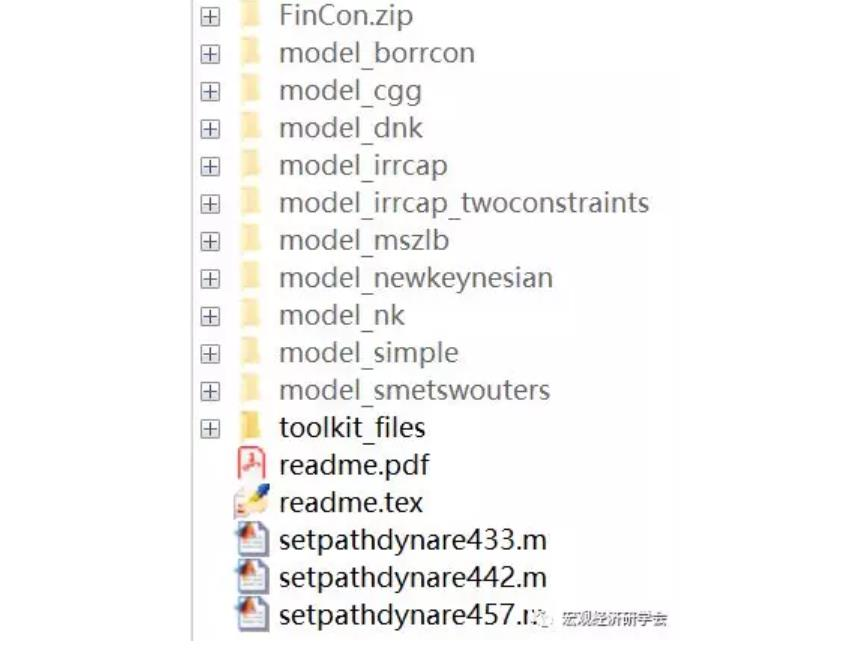
\includegraphics[width=0.5\linewidth]{FIG/folders}
	\centering
\end{figure}

\begin{itemize}
	\item 
	setpathdynareXXX.m file is a file that sets the path of dynare and OccBin. Generally speaking, we need to add Dynare-matlab and OccBin-toolkit\_files to the default path of matlab. After the file is opened, it looks like this:
	\begin{figure}[htbp!]
		\centering
		
\includegraphics[width=0.8\linewidth]{FIG/setpathoccbin}
		\centering
	\end{figure}
	\begin{enumerate}
		\item We need to change the local user name in the computer, for example, my computer local user name is "wenli xu", so I changed the single quote on line 3 to \textbf{location=}\textcolor{red}{'wenli xu '};
		\item Match the characters on line 10 and change them accordingly to 'wenli xu';
		\item Set line 11 path 1 to the location of the matlab subfolder in our installed Dynare, for example dir1='C:/metering/4.5.7/4.5.7/matlab';
		\item Set path 3 on line 13 to the location of the toolkit\_files subfolder in our installed OccBin, for example dir3='C:/Users/xuwen/OneDrive/Paper Replication Code/occbin\_20140630/occbin\_20140630/ toolkit\_files';
		\item Save the file, run the file, either click the run button, or enter the file name in the command window of matlab: >>setpathdynare457, press Enter.
	\end{enumerate}
	
	However, I strongly recommend not using this method to add paths, as it would require re-running setpathdynare457 after every restart of matlab.
	
	\textbf{Recommended: Click directly on the matlab menu bar setpath---Add with Subfolders---toolkit\_files---save.}
\end{itemize}

In addition to the setpathdynare file and the toolkit\_files folder, there are other folders, which are our custom model files, including mod files, steady state files and simulation files. Let's take the above ZLB model as an example:

\begin{itemize}
	\item We create a new folder model\_nk
	
	\begin{figure}[htbp!]
		\centering
		
\includegraphics[width=0.8\linewidth]{FIG/modelnk}
		\centering
	\end{figure}
	
	\textcolor{red}{Two key steps of OccBin:}
	
	\textbf{The first step is to write two .mod files, one is the model without ZLB constraints (such as nk.mod), and the other is the model with ZLB constraints (such as nk\_zlb.mod).}
	\begin{itemize}
		\item In the unconstrained model, it is the same as we usually write mod files. It should be noted that ZLB has no constraints at this time, so the monetary policy rules are still written as Taylor rules:
		
		\begin{figure}[htbp!]
			\centering
			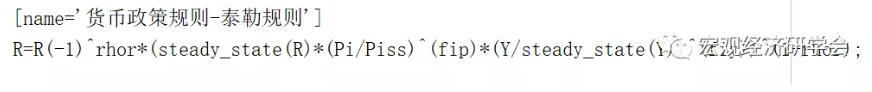
\includegraphics[width=0.8\linewidth]{FIG/TR}
			\centering
		\end{figure}
		
		\item In the constrained model mod file, you only need to keep the var, varexo, parameters, model modules in the above benchmark mod. And the monetary policy rule is now a constant:
		\begin{figure}[htbp!]
			\centering
			
\includegraphics[width=0.8\linewidth]{FIG/TRconstant}
			\centering
		\end{figure}
	\end{itemize}
	
	\textbf{The second step is to write a separate .m file, in this file, we need to declare the constraints (in the form of linearization), and then call the OccBin toolkit functions to solve, simulate the constrained and unconstrained models. For example, we write the runsim\_newkeynesian.m file.}
	
	\begin{figure}[htbp!]
		\centering
		
\includegraphics[width=0.8\linewidth]{FIG/mfile}
		\centering
	\end{figure}
	
	We can look at the program of this file:
	
	\textbf{(1) Declare global variables: }\textcolor{red}{M\_、oo\_}, if you are familiar with Dynare output, the two global variables M\_ and oo\_ refer to the endogenous/exogenous/parametric variable names of the model, and the simulation result variables (including steady state, simulation values, etc.)
	
	\begin{lstlisting}[frame=shadowbox]
		\textcolor{red}{M\_~oo\_}
	\end{lstlisting}
	
	Declaring global variables allows mods of the alternative model to invoke the parameters of the baseline model, as well as the simulation results, etc. Recall that in the alternative model mod file, only the var, varexo, parameters and model modules are included. Therefore, these global variables need to be fed back into the alternative model.
	
	\textbf{(2) Declare the mod filenames of the baseline model and the alternative model:}
	
	\begin{lstlisting}[frame=shadowbox]
		modnam = 'nk';
		modnamstar = 'nk\_zlb';
	\end{lstlisting}
	
where modnam represents the mod filename of the baseline model, and modnamstar represents the mod filename of the alternative model. Since in our ZLB-DSGE case, the baseline model is without ZLB constraints, the alternative model is with ZLB constraints.
	
	\textbf{(3) Declare constraints:}
	
	\begin{lstlisting}[frame=shadowbox]
		constraint = \textcolor{red}{'R<RZLB-Piss/betta'};
		constraint_relax =\textcolor{red}{'R>RZLB-Piss/betta'};
	\end{lstlisting}
	
	Among them, constraint represents the condition that the constraint holds; constraint\_relax indicates the condition that the constraint does not hold.
	
	In the above example,
	\begin{itemize}
		\item The original ZLB constraints are:
		$$R_t<R^{ZLB}=1$$
		\item \textcolor{red}{It is important to note that in the above constraint declaration, the variables must be rewritten to the linear form they appear in the Dynare solution. In general, this depends on how we declare the model form (eg levels, log-levels, etc.) in the model module of the mod file. In our example above, we declared the model in a non-linear form, therefore, we need to convert the constraints to a linear form, i.e. $\hat{X}_t=X_t-X$($\hat{X}_t $ represents the linearized variable, X represents the steady-state value);}
		\item Therefore, we need to express the ZLB constraint as
		$$R_t=\hat{R}_t+R<R^{ZLB}$$
		$$\hat{R}_t<R^{ZLB}-R$$
		\item Therefore, when declaring constraints we can see that:
		
		\begin{lstlisting}[frame=shadowbox]
			constraint = \textcolor{red}{'R<RZLB-Piss/betta'};
			constraint_relax =\textcolor{red}{'R>RZLB-Piss/betta'};
		\end{lstlisting}
	\end{itemize}
	
	\textbf{(4) When the program judges that the constraint is true, the solution of the model is converted from the reference model to the alternative model, that is, run nk\_zlb; when the constraint\_relax is true, the solution is run nk.}
	
	\textbf{(5) Assign the exogenous shock variable in the .mod file to irfshock:}
	
	\begin{lstlisting}[frame=shadowbox]
		irfshock =char('e_a','e_u');
	\end{lstlisting}
	
	Since the exogenous shocks in the above example are e\_a and e\_u, two shocks are declared above.
	
	\textbf{(6)在shockssequence声明不可预期冲击序列,且在nperiods 声明IRF期数:}
	
	\begin{lstlisting}[frame=shadowbox]
		SHOCKS = [ zeros(5,2)
		0  0.024
		zeros(20,2) ] ;
		
		
		shockssequence = SHOCKS;
		nperiods = 30;
	\end{lstlisting}
	
	\textbf{(7) Solve the model by the following command and get the IRFs:}
	
	\begin{lstlisting}[frame=shadowbox]
		[zdatalinear zdatapiecewise zdatass oobase_ Mbase_  ] = ...
		solve_one_constraint(modnam,modnamstar,...
		constraint, constraint_relax,...
		shockssequence,irfshock,nperiods);
	\end{lstlisting}
	
      where  the ellipsis indicates a newline.
	\begin{itemize}
		\item zdatalinear: When OBCs are ignored, the dynamic paths of endogenous variables are simulated, expressed as steady-state deviations. Each column represents a variable, in the order of the variables declared in the mod file;
		
		\item zdatapiecewise: When OBCs hold, the dynamic paths of endogenous variables are simulated. The same order as above;
		
		\item zdatass: Steady-state values of endogenous variables;
		
		\item oobase\_ and Mbase\_ : See the manual for the structure Dynare produces when running the benchmark model.
	\end{itemize}
	
	\textbf{(8) Enter in the matlab command window:}>>\textcolor{red}{runsim\_newkeynesian}, the following impulse response graph can be obtained.
	
	
	\begin{figure}[htbp!]
		\centering
		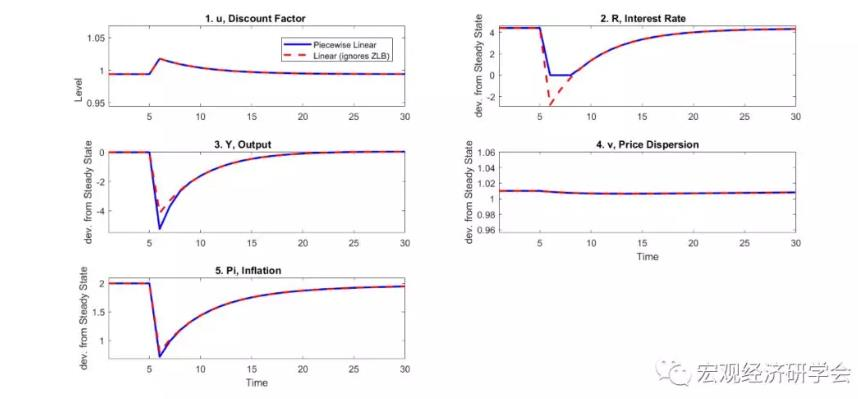
\includegraphics[width=0.8\linewidth]{FIG/occbinirf}
		\centering
	\end{figure}
	
	We can clearly see the change in the nominal interest rate (blue line) when the ZLB constraint holds in Figure 2 above.
\end{itemize}

IV. Precautions

We have introduced the basic principles and operations of OccBin earlier. But there are still some things that need special attention.
\begin{enumerate}
	
	\item When declaring constraints, OccBin only allows the use of linearized constraints;
	
	\item Only contemporaneous endogenous variables are allowed in constraint and constraint\_relax. For example, if the mortgage constraint $b_t\le\rho_tq_th_t$ is $b_t\le\rho_tq_th_{t+1}$, then this condition cannot be directly entered into constraint and constraint\_relax, we should first convert $h_{t+1}$ with lead\_. The same is true for lag periods. See the dynare manual for lead lag transitions.
	
	\item The steady state of the alternative model does not need to be declared. Both the base model and the alternative model approximate the steady state of the base model. The baseline model needs to satisfy the BK condition, while the alternative model does not need to satisfy the BK condition.
	
	\item Parameters only need to be assigned values in the baseline model, but not in the alternative model. If the parameter only appears in the alternative model (such as $R^{ZLB}$ in the above example), we also need to declare the parameter in the baseline model and assign it.
	
\end{enumerate}


Furthermore, OccBin has a very important connection to the mechanism transfer model:
\begin{itemize}
	\item When there is a mechanism conversion, OccBin does not deliver policy rules, it is 100$\%$ consistent with the model. Because OccBin assumes that agents cannot predict binding bindings, it also does not form expectations about when to enter or exit OBCs.
	
	\item However, in some macroeconomic studies, agent expectations about mechanism transfer are also very interesting and have very important macroeconomic implications. Therefore, many scholars are also interested in quantifying this expectation, which is the MS-DSGE model.
	
\end{itemize}

Andrew Binning and Junior Maih (2017) regard OBCs as a special kind of RS and use Regime-Switching to model OBCs. Later, we will introduce this method.
V. Summary

When the expression $stoch\_simul()$ is used in the .mod file, Dynare computes a Taylor approximation of the decision and transition functions of the model. This is computed around the steady state and at first order will be of the form

$$y_t=y+A(y_{t-1}-y)+Bu_t$$

where y is the steady state value of $y_t$. It is worth pointing out here that if we wanted to include an inequality constraint in a model such as

\begin{equation*}
	y_t=
	\begin{cases}
		f(x_t),& when f(x_t)\ge0\\
		0,\space &otherwise
	\end{cases}
\end{equation*}

then although possible to write the function $y = max(fx,0)$, if $stoch\_simul()$ is used, Dynare will perform a local approximation around the deterministic steady state. The equation will then either be a approximation of $y_t = f(x_t)$ or $y_t = 0$ depending on whether the constraint binds in steady state. The inequality constraint will be lost.

The approach generalises to higher orders and up to order three is available in Dynare. For further reading on the technical detail for the derivation of policy function and the higher order equivalents, we refer the reader to Collard and Juillard (2001).

Whilst the perturbation techniques employed by Dynare to solve stochastic models lose this type of constraint, the same is not true for perfect foresight or extended path solutions.


\subsection{Extended\_Path Approach}

As write in the manual:

The use of the following functions and operators is strongly discouraged in a stochastic context: max, min, abs, sign, <, >, <=, >=, ==, !=. The reason is that the local approximation used by stoch\_simul or estimation will by nature ignore the non-linearities introduced by these functions if the steady state is away from the kink. And, if the steady state is exactly at the kink, then the approximation will be bogus because the derivative of these functions at the kink is bogus (as explained in the respective documentations of these functions and operators).

Note that \textbf{extended\_path} is not affected by this problem, because it does not rely on a local approximation of the model.

It is possible to compute a simulation to a stochastic model using the extended path method presented by Fair and Taylor (1983). This method is especially useful when there are strong nonlinearities or binding constraints. Such a solution is computed using the $extended\_path$ command.

I. Basic idea

The extended path approach, introduced by Fair and Taylor (1983), relies on the perfect foresight model solvers to take full account of the deterministic nonlinearities (either related to the preferences or technology functional forms, or to the presence of occasionaly binding constraints).

\begin{itemize}
	\item In each period of the sample, exogenous innovations are treated as surprise shocks in the first period of a deterministic simulation where shocks are set to their expected value in all future periods.
\end{itemize}

The advantages of this approach,compared to other global approximation methods, is that

\begin{itemize}
	\item it allows to simulate very large models (like a multicountry model with thousands of equations).
	\item this approach is not model dependent, as other global approximation methods, it does not require more work than writting the equations of the model in a Dynare’s .mod file.
\end{itemize}

II. Algorithm

\textbf{Perfect Foresight Solutions}

When $simul()$ is used in the .mod file, Dynare uses a Newton-type algorithm which preserves these non-linearities. Details of the algorithm can be found at Juillard (1996). In such a model, the economy is in equilibrium up until period 1 at which point the agents learn about any shocks in the current or
future periods. The simulation then describes the response of the agents before and following any shocks, until the economy returns to equilibrium. This equilibrium may or may not be the same as the initial one before period 1 and the path to equilibrium is imposed in finite time rather than asymptotically.

As using a deterministic set-up allows the analysis of the full implications of non-linearities, it is a useful starting point.

Suppose there were no past shocks and will be no future shocks so no uncertainty; we can write the borrowing constraints model from above:

$$\dbinom{...}{min\{\rho_t,(mq_th_t^i-b_t^i)\}}=0$$

or

$$f(x_{t-1},x_t,x_{t+1},u_t)=0$$

where $x_t$ is the endogenous state and $u_t$ are exogenous shocks.

A perfect foresight solution given initial $u_1$, starting from $x_0$ is a path $x_0; x_1; x_2;$ ... converging to steady state and satisfying:

$$f(x_0,x_1,x_2,u_1)=0$$

$$f(x_1,x_2,x_3,0)=0$$

$$f(x_2,x_3,x_4,0)=0$$

$$...$$

Dynare's perfect foresight solver can be used for calculating perfect foresight IRFs.

To do this, in the shocks block we specify the initial impulse, e.g.:

\begin{figure}[htbp!]
	\centering
	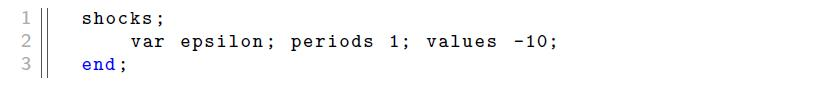
\includegraphics[width=0.8\linewidth]{FIG/extendpath}
	\centering
\end{figure}

where the number after values specifies the size of the initial impulse.

And then we perform the simulation with:

\begin{figure}[htbp!]
	\centering
	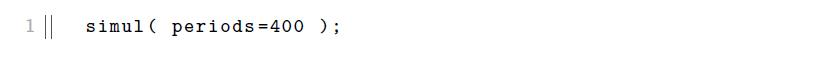
\includegraphics[width=0.8\linewidth]{FIG/runsimul}
	\centering
\end{figure}

To solve, this is stacked over T periods

\begin{figure}[htbp!]
	\centering
	
\includegraphics[width=0.8\linewidth]{FIG/equationsexpath}
	\centering
\end{figure}

Initial and end conditions given ($x_0 = x_{T+1}= \hat{x}$)

From an initial guess at n = 0, solve the following, updating x until suffcient accuracy is achieved.

$$x_{n+1}=x_n-\frac{f(x_n)}{f'(x_n)}$$

Dynare uses steady state for initial guesses.

Dynare stores the output of perfect foresight simulations in: $oo\_.endo\_simul$

\textbf{(Stochastic) Extended-Path Algorithm}

Dynare (i) draws a random path for all exogenous variables then (ii) computes the corresponding path for the endogenous variables using the algorithm:

\begin{enumerate}
	\item An integer k is chosen which is the number of periods for which expectations must be computed.
	\item Beginning with expectations equal to the steady-state values $E_sx_{s+r} = x$ for r = 0,..., k, obtain a new set of expectations by solving the non-linear model dynamically. Every period the expectations are evaluated using a Gaussian quadrature.
	\item Setting the new expectations as the starting values, this is repeated until convergence.
	\item Repeat the above but increasing r by 1 and repeat this until convergence.
\end{enumerate}

The solution method builds on the underlying perfect foresight algorithm of the last section, the difference being that $E_t\left[\{x_{t+s}\}_{s=1}^k\right]$ will not necessarily equal $\{x_{t+s}\}_{s=1}^k$.

This captures the non-linearities of the system and differs from the standard stochastic simulation which computes approximations to the transition and policy equations.

三、Dynare Command

we use the New Keynesian model with a zero lower bound on nominal interest rates from Fernández-Villaverde et al. (2015) as given in the provided code. The equilibrium conditions are outlined

$$\frac{1}{C_t}=E_t\frac{\beta}{C_{t+1}}\frac{R_t}{\Pi_{t+1}}$$

$$W_t=\psi L_t^{\vartheta}C_t$$

$$MC_t=\frac{W_t}{A_t}$$

$$\epsilon X_{1,t}=(\epsilon-1)X_{2,t}$$

$$X_{1,t}=\frac{1}{C_t}MC_tY_t+\theta E_t\beta \Pi_{t+1}^{\epsilon}X_{1,t+1}$$

$$X_{2,t}=\Pi_t^{\star}\left(\frac{Y_t}{C_t}+\theta E_t \beta \frac{\Pi_{t+1}^{\epsilon-1}}{\Pi_{t+1}^{\star}}X_{2,t+1}\right)$$

$$R_t=max(1,Z_t)$$

$$Z_t=R^{1-\rho_r}R_{t-1}^{\rho_r}\left[\left(\frac{\Pi_t}{\Pi}\right)^{\phi_{\pi}}\left(\frac{Y_t}{Y}\right)^{\phi_y}\right]^{1-\rho_r}M_t$$

$$G_t=S_{g,t}Y_t$$

$$1=\theta\Pi_t^{\epsilon-1}+(1-\theta)\Pi_t^{\star~1-\epsilon}$$

$$v_t=\theta\Pi_t^{\epsilon}v_{t-1}+(1-\theta)\Pi_t^{\star~-\epsilon}$$

$$Y_t=C_t+G_t$$

$$Y_tv_t=A_tL_t$$

In Dynare this is easy to implement. $Z_t$ can be specified as a model-local variable1 by leaving it out of the variable declarations at the beginning of the mod file and entering ‘\#’ before the equation in the ‘model’ section. The Taylor-type rule can then be expressed in the .mod file

\begin{lstlisting}[frame=shadowbox]
	
	model;
	.
	.
	.
	#z=rho_r*r(-1) + (1 - rho_r)*( r_bar + phi_pi*...
	( pi - pi_bar ) + phi_y*( y - y_bar ) + m;
	r=max(0,z);
	.
	.
	.
	end;
	
\end{lstlisting}

\textbf{Deterministic Model}
\begin{itemize}
	\item $simul(lmmcp);$
	
	Solves the perfect foresight model with a Levenberg-Marquardt mixed complementarity problem (LMMCP) solver (Kanzow and Petra 2004), which allows to consider inequality constraints on the endogenous variables (such as a ZLB on the nominal interest rate or a model with irreversible investment). This option is equivalent to stack\_solve\_algo=7 and solve\_algo=10. Using the LMMCP solver requires a particular model setup as the goal is to get rid of any min/max operators and complementary slackness conditions that might introduce a singularity into the Jacobian. This is done by attaching an equation tag (see Section 4.5 [Model declaration], page 20) with the mcp keyword to affected equations. This tag states that the equation to which the tag is attached has to hold unless the expression within the tag is binding. For instance, a ZLB on the nominal interest rate would be specified as follows in the model block:
	
	\begin{lstlisting}[frame=shadowbox]
		model;
		...
		[mcp='r>-1.94478']
		r = rho*r(-1) + (1-rho)*(gpi*Infl+gy*YGap) + e;
		...
		end;
	\end{lstlisting}
	
	where 1.94478 is the steady state level of the nominal interest rate and r is the nominal interest rate in deviation from the steady state. This construct implies that the Taylor rule is operative, unless the implied interest rate r<=-1.94478, in which case the r is fixed at -1.94478 (thereby being equivalent to a complementary slackness condition). By restricting the value of r coming out of this equation, the mcp-tag also avoids using max(r,-1.94478) for other occurrences of r in the rest of the model. It is important to keep in mind that, because the mcp-tag effectively replaces a complementary slackness condition, it cannot be simply attached to any equation. Rather, it must be attached to the correct affected equation as otherwise the solver will solve a different problem than originally intended.
	
	Note that in the current implementation, the content of the mcp equation tag is not parsed by the preprocessor. The inequalities must therefore be as simple as possible: an endogenous variable, followed by a relational operator, followed by a number (not a variable, parameter or expression).
	
\end{itemize}

\textbf{Example}

We focus first on the government spending shock. The model is in deterministic steady state until period one at which point the government cuts spending $G_t$ as a proportion of GDP by nearly half, sustaining the cuts for five periods before returning spending level to the original steady state value. The shock
specification is detailed

\begin{lstlisting}[frame=shadowbox]
	
	shocks;
	var epsilon_Sg;
	periods 1:5;
	values 100;
	end;
	
\end{lstlisting}

Note that we have also altered the persistence $\rho_g$ of the shock to zero, and set the variance $S_g$ equal to 1. This is
equivalent to ensuring the government spending is determined by the equation

$$S_{g,t}=S_g+\epsilon_{g,t}$$

where $S_{g,t}$ is the size of government spending relative to output and Sg = 20\% is the steady state value. During this time, the shadow interest rate becomes negative and so the nominal interest rate is constrained at zero. This can be
seen in figure 4.1.

\begin{figure}[htbp!]
	\centering
	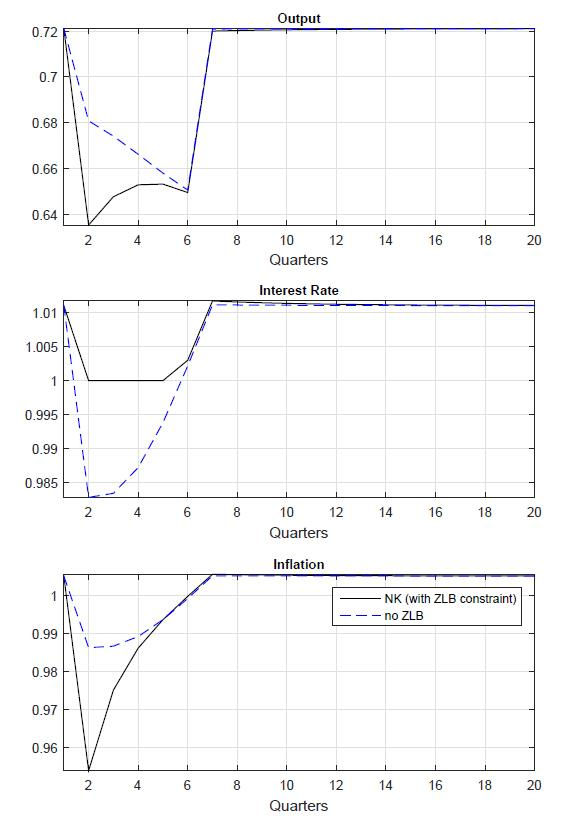
\includegraphics[width=0.8\linewidth]{FIG/simul}
	\caption{Perfect foresight impulse response function following negative demand shock}\label{4.1}
	\centering
\end{figure}

Disadvantages:

\begin{itemize}
	\item Captures full non-linearities including OBCs;
	\item However, heavy computational demand so can be slow and unstable. Particularly if equations not differentiable everywhere-as with OBCs
	
	The model is solved by stacking the system over T periods, where T is large enough to return the system to equilibrium. The Newton approach solves all the equations over every period simultaneously. This approach leads to a very large Jacobian; for a simulation over T periods, a model with n endogenous variables will require a Jacobian matrix of order n * T leading to high computational demands.
	\item the role of uncertainty in the behaviour of agents is lost. Fails to capture risk and precautionary behaviour.
	\item Also, The choice of solution can be a problem; it is unclear if there are multiple solutions to the model and why the one returned is chosen. It may not converge to a solution and(i)if it doesn't, we don't know it is because there isn't one,(ii)if it does, we don't know if it is unique.
	
\end{itemize}


\textbf{随机模型}

Shocks are specified as when using stoch\_simul, but instead use:

\begin{itemize}
	\item $extended\_path;$
	\item $extended\_path(OPTIONS...);$
	
	\textbf{Description}
	
	extended\_path solves a stochastic (i.e. rational expectations) model, using the extended path method presented by Fair and Taylor (1983). Time series for the endogenous variables are generated by assuming that the agents believe that there will no more shocks in the following periods.
	
	This function first computes a random path for the exogenous variables (stored in oo\_.exo\_simul, page 46) and then computes the corresponding path for endogenous variables, taking the steady state as starting point. The result of the simulation is stored in oo\_.endo\_simul, page 46). Note that this simulation approach does not solve for the policy and transition equations but for paths for the endogenous variables.
	
	\textbf{OPTIONS}
	\begin{itemize}
		\item $periods = INTEGER$
		
		The number of periods for which the simulation is to be computed. No default value, mandatory option.
		
		\item $solver\_periods = INTEGER$
		
		The number of periods used to compute the solution of the perfect foresight at every iteration of the algorithm. Default: 200.
		
		\item $order = INTEGER$
		
		If order is greater than 0 Dynare uses a gaussian quadrature to take into account the effects of future uncertainty. If order=S then the time series for the endogenous variables are generated by assuming that the agents believe that there will no more shocks after period t+S. This is an experimental feature and can be quite slow. Default: 0.
		
		\item $hybrid$
		
		Use the constant of the second order perturbation reduced form to correct the paths generated by the (stochastic) extended path algorithm.
	\end{itemize}
	
	
\end{itemize}

When the command $extended\_path(order=k,periods=T)$ is used, Dynare first draws a random path for the exogenous variables over T periods before computing the corresponding path for endogenous variables, taking the steady state as starting
point. The order k specifies the number of periods ahead for which agents believe shocks may occur.

At order 0, this creates a stochastic simulation as if only the shocks of the current period were random, meaning that this is just a stochastic version of the standard perfect foresight solution method. As this neglects Jensen’s inequality, uncertainty plays no role in the model.

In practice, the extended-path method in dynare doesn't solve the full rational expectations model. The modeller specifies the maximum value of k for which to solve using the order option (k-level thinking).

By increasing the order, the number of periods of uncertainty
considered are increased. For example at order one, the algorithm allows for shocks next period, but assumes no shocks will arrive in two periods’ time, at order 2, two periods of future shocks are allowed for, and so on. The approximation
is solved by integrating over the shocks up to the specified horizon. Beyond this time horizon, the assumption is that all shocks will for evermore be zero and so consequently the model will ignore the long-run risk of hitting the bound.

For example, if order =2 were entered, dynare would only compute expectations as if shocks could be non-zero for 2 more periods. After this horizon, the agents would believe that there would be no more future shocks.

\textbf{例子}

To solve the NK model, we set the order k = 0 and periods T = 1000. Figure 4.2 shows the paths of the interest rate, output and inflation over 100 periods

\begin{figure}[htbp!]
	\centering
	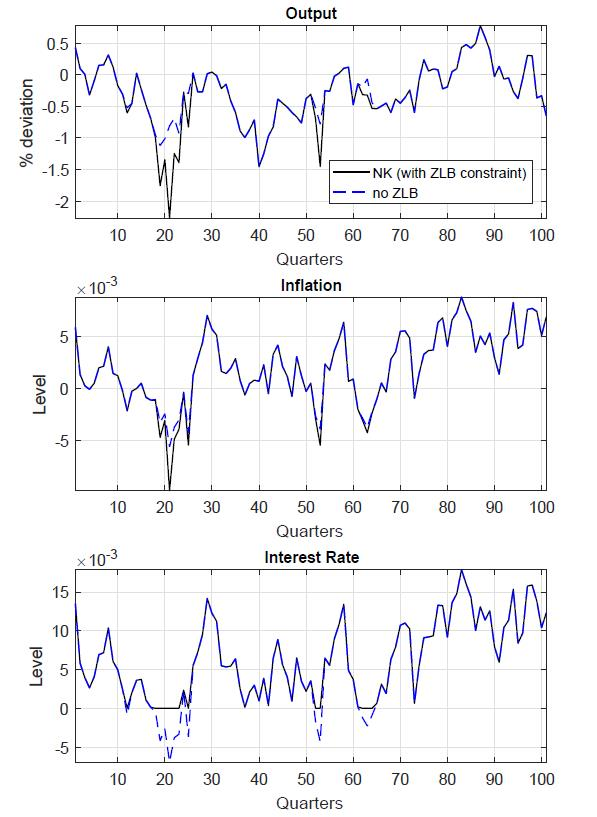
\includegraphics[width=0.8\linewidth]{FIG/extendedpath}
	\caption{Extended-Path simulations (order = 0)}\label{4.2}
	\centering
\end{figure}

At order zero there is neither future uncertainty nor precautionary behaviour. Up to the period the constraint binds and immediately after, the paths of the variables are identical as the agents ignore any risk of the constraint binding in
future. To deal with this, it would be necessary to increase the order and allow the agents to evaluate future uncertainty. We find that by doing so, the model becomes prohibitively slow to solve.

\begin{itemize}
	\item For accuracy, the order should be set to be the same magnitude as the decay of the model.
	\item dynare uses Gaussian quadrature to evaluate the expectations which scales exponentially in the number of shocks and the order (although not the number of states).
	\item In practice, solving with sufficient accuracy is infeasible except for very small models.
	
\end{itemize}


\subsection{News Shocks Approach}

As described in the above, there are a number of methods for solving larger models with OBCs including fast ones (such as Guerrieri and Iacoviello (2015b)) and accurate ones (such as Maliar and Maliar(2015)).

In this section, we will introduce the News shocks method\footnote{参见DSGE建模与编程入门(44):ZLB与News Shocks。News Shocks更加详细的信息可以参考Barsky and Sims(2011,JME)、Born et al. (2013,JEDC)和Barsky et al. (2015,Whither News Shocks?)等。} proposed in Holden (2016a,b) which provides a balance between accuracy and speed in simulation. For detail of the method, we direct the reader to a theoretical paper on the existence and uniqueness condition in Holden (2016b), and a paper detailing the computational algorithm in Holden (2016a).

\textbf{Idea: use news shocks to impose the bounds, and an endogenous source of information about the constraint which can be predicted.}

\begin{itemize}
	\item If an OBC would otherwise be violated, anticipated news shocks push the constrained variable(s) back to their bound.
	\item A shock that drives a variable to its bound for an episode can be thought of as a combination of the original shock and a sequence of news shock stating that the variable will be higher than expected for some duration.
\end{itemize}

As showed in Figure 4.3

\begin{figure}[htbp!]
	\centering
	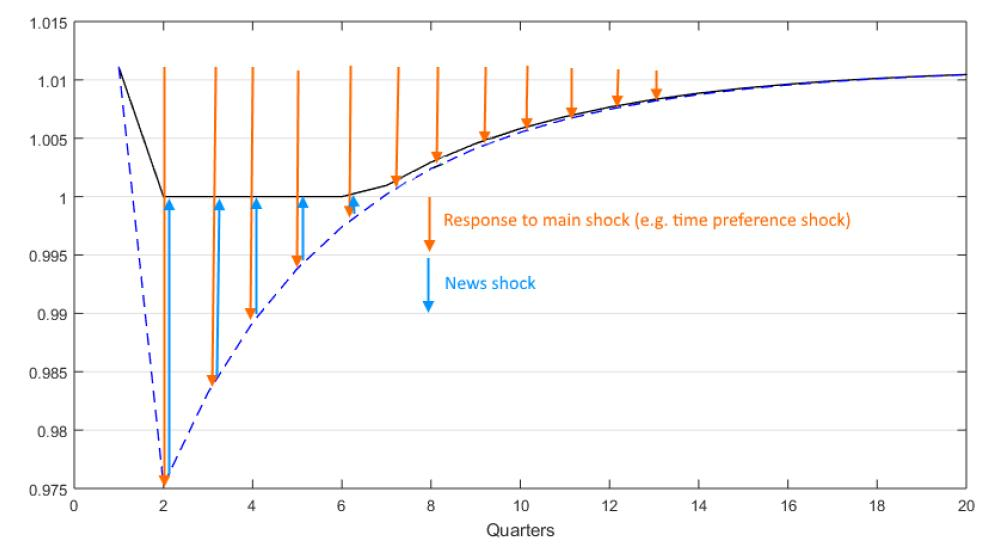
\includegraphics[width=0.8\linewidth]{FIG/newsshock}
	\caption{Holden(2016) news shocks method}\label{4.3}
	\centering
\end{figure}

The algorithms are designed to be easily implemented into Dynare. The occasionally binding constraint tool-kit DynareOBC needs to be downloaded and added to the Matlab path. The tool-kit is available from

\url{https://github.com/tholden/dynareOBC}

DynareOBC works best if you have admin rights on your own machine, so it may install dependencies automatically. If you dont have admin rights, the ReadMe file contains details of what your IT administrator must install for you.

Once downloaded, the root DynareOBC folder, containing dynareOBC.m, needs to be added to the your Matlab path.

You can read information on the tool-kit by typing dynareOBC into the MATLAB command window. The first step is to test the Dynare installation by typing:

\begin{lstlisting}[frame=shadowbox]
	>> dynareOBC testsolvers
\end{lstlisting}

which will attempt to solve a number of computational problems and check whether the required solvers are working correctly.

After running TestSolvers, it is a good idea to clean up the path using:

\begin{lstlisting}[frame=shadowbox]
	>> dynareOBC rmpath
\end{lstlisting}

\begin{figure}[htbp!]
	\centering
	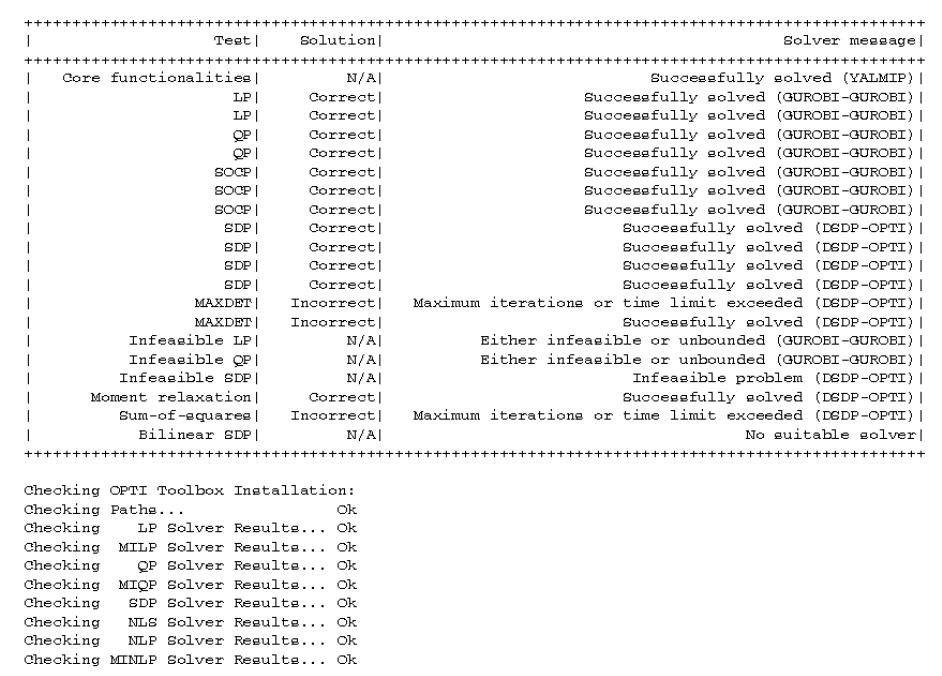
\includegraphics[width=0.8\linewidth]{FIG/rmpath}
	\centering
\end{figure}

\subsubsection{the basics of dynareOBC usage}

The bounded variable simply has to be written in the .mod file as we have above. For example, to have interest rates set by a Taylor rule but bounded at zero, dropping the model-local variable $z_t$, we include the equation as shown
in the following listing

\begin{lstlisting}[frame=shadowbox]
	r = max( rho_r*r(-1) + (1 - rho_r)*( r_steady + phi_pi*(pi -
	pi_steady) + phi_y*(y - y_steady) ) + m,0);
\end{lstlisting}

The model is then run from the MATLAB command window with the command \textbf{$dynareOBC [FILENAME].mod [OPTIONS]$}. It should be noted that not all stoch\_simul options are supported by dynareOBC, and currently no warning will be generated if unsupported options are used.

Suppose you have the NK ZLB model defined in the file NK\_ZLB.mod. Typing

\begin{lstlisting}[frame=shadowbox]
	>> dynareOBC NK_ZLB.mod shockscale=10
\end{lstlisting}

will simulate the model without using cubature. If \textcolor{blue}{irf}=40 or some other positive integer, IRFs will computed, and if, for example, \textcolor{blue}{periods}=1000 then the model will use the extended-path type method to simulate the model over 1000
periods. The option \textcolor{blue}{shockscale}=10 scales up the IRF shock by a factor of 10. Note that when you list options after the model file name that have ‘=’ you
must make sure to not include spaces around the equals sign. The options are not case sensitive.

If IRFs are computed, unless otherwise specified in the \textcolor{blue}{$stoch\_simul()$} command, you will see the IRF plots which have the paths with (solid line) and without (dotted line) the bounds. Figure 4.4 shows the plots again for output, inflation and the interest rate. As usual, the IRFs are stored in $oo\_.irfs$.

\begin{figure}[htbp!]
	\centering
	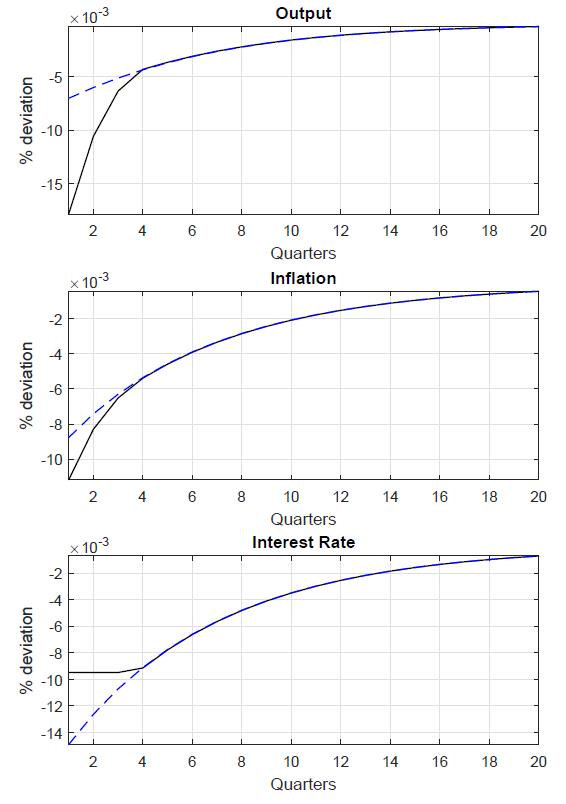
\includegraphics[width=0.8\linewidth]{FIG/dynareOBC}
	\caption{dynareOBC IRF simulation without cubature}\label{4.4}
	\centering
\end{figure}

In addition to the $oo\_.$ and $M\_.$ structures, dynareOBC stores results and data in a structure $dynareOBC\_.$. For instance, the IRFs without the bounds are stored in $dynareOBC\_.IRFsWithoutBounds$, and the M matrix is stored in $dynareOBC\_.MMatrix$.

\subsubsection{Estimation of Models with OBCs}

Traditional linear DSGE models are estimated using the Kalman filter. This gives a very computationally efficient way to evaluate the exact likelihood of a linear-Gaussian model. I.e., given guesses for the parameters of the model, the Kalman filter returns the probability density of observing what we did, given those parameters. Unfortunately, the derivation of the Kalman filter relies on the special properties of linear models with Gaussian shocks, and once any non-linearity is introduced, the Kalman filter is no longer applicable.

In a non-linear world then, an another approach must be taken. Here, we propose one which returns an approximation to the likelihood that requires relatively few simulation steps of the non-linear model, without overly distorting the shape of the likelihood function. Given how computationally expensive
it is to simulate a DSGE model with an occasionally binding constraint, minimising the amount required is crucial for our application.

The central trick of the cubature Kalman filter approach is that for many non-linear models, even after having made several observations, the distribution of the state variables conditional on the parameters and on our observations is still approximately Gaussian. Thus although the distribution of the
state will never be exactly Gaussian in a non-linear world, perhaps we will not lose to much if we nonetheless assume that it is.

DynareOBC includes built in code implementing the cubature Kalman filter. This enables the estimation of models with or without occasionally binding constraints, at up to a third order approximation. We will test this facility on a simple RBC model with irreversible investment, inelastic labour supply, and productivity known one period in advance.

We simulate some data from the model by changing to the Estimation folder. IrrevInv.mod is the file shown in the following listing:

\begin{lstlisting}[frame=shadowbox]
	1 var a M k r;
	2 
	3 varexo epsilon;
	4 
	5 parameters alpha beta delta mu sigma;
	6
	7 alpha = 0.3;
	8 beta = 0.99;
	9 delta = 0.0025;
	10 mu = 0;
	11 sigma = 0.075;
	12
	13 model;
	14 #A = exp( a );
	15 #LAG_A = exp( a(-1) );
	16 #LEAD_K = exp( k(+1) );
	17 #K = exp( k );
	18 #LAG_K = exp( k(-1) );
	19 #I = K - ( 1 - delta ) * LAG_K;
	20 #LEAD_I = LEAD_K - ( 1 - delta ) * K;
	21 #C = LAG_A ^ ( 1 - alpha ) * LAG_K ^ alpha - I;
	22 #LEAD_C = A ^ ( 1 - alpha ) * K ^ alpha- LEAD_I;
	23 #R = exp( r );
	24 a = mu + sigma * epsilon;
	25 I - C * ( C + I ) * M = C * ( C + I ) * beta * ( 1 / LEAD_C * 
	(alpha * A ^ ( 1 - alpha ) * K ^ ( alpha - 1 ) + 1 - delta
	) - ( 1 - delta ) * M(+1) ) - C;
	26 I = max( 0, C * ( C + I ) * beta * ( 1 / LEAD_C * ( alpha *
	A ^( 1 - alpha ) * K ^ ( alpha - 1 ) + 1 - delta ) - ( 1 -
	delta ) * M(+1) ) - C );
	27 1 / C = beta * R / LEAD_C;
	28 end;
	29
	30 steady_state_model;
	31 a = mu;
	32 M = 0;
	33 k = mu + 1 / ( alpha - 1 ) * log( ( 1 / beta - ( 1 - delta ) )
	/ alpha );
	34 r = -log( beta );
	35 end;
	36
	37 shocks;
	38 var epsilon = 1;
	39 end;
	40
	41 steady;
	42 check;
	43
	44 stoch_simul( pruning, order = 3, irf = 0, periods = 500 ) C I R;
\end{lstlisting}

Typing in Matlab command:

\begin{lstlisting}[frame=shadowbox]
	>> dynareOBC IrrevInv.mod mlvsimulationmode=1
	compilesimulationcode nocubature
\end{lstlisting}

After dynareOBC completes, we extract and save the resulting simulations (discarding the first 100 periods) using the code:

\begin{lstlisting}[frame=shadowbox]
	1 mlv = dynareOBC_.MLVSimulationWithBounds;
	2 data = [ mlv.C', mlv.I', mlv.R' ];
	3 data = data( 101:500, : );
	4 xlswrite( 'IrrevInvTemp.xlsx', data );
\end{lstlisting}

While native Dynare relies on the \textcolor{blue}{estimated\_params} and \textcolor{blue}{estimation} sections of the .mod file for specifying what exactly needs to be estimated, dynareOBC gets all of this information from the Excel spreadsheet containing the data. DynareOBC expects the Excel spreadsheet to contain two worksheets within it, where the first one has the names of the endogenous variables in the first row, and data in subsequent rows, and where the second contains the names of the
parameters to be estimated in the first row, and their lower and upper bounds in the second and third rows respectively (with empty cells being interpreted as unbounded). Thus, we open IrrevInvTemp.xlsx in Excel and insert a new row into the top of the first sheet containing:

\begin{table}[htbp!]
	\centering
	\begin{tabular}{ccc}
		\hline
		C&I&R\\
		\hline
	\end{tabular}
\end{table}

We then insert a second worksheet, containing the data:
\begin{table}[htbp!]
	\centering
	\begin{tabular}{ccccc}
		\hline
		alpha &beta &delta &mu &sigma\\
		\hline
		0&0&0&&0\\
		1&1&1&&\\
		\hline
	\end{tabular}
\end{table}

This specifies all parameters except $\sigma$ to be bounded between 0 and 1, while $\sigma$ is just constrained to be positive. We then save the result as $IrrevInv.xlsx$. By default, when dynareOBC’s $estimation$ command line option is specified, dynareOBC automatically looks for a file with the same name as the .mod file, but with an .xlsx extension. Hence, with this file name, the data will be loaded automatically by dynareOBC. Alternatively, an explicit filename may be provided
to dynareOBC with the $EstimationDataFile=FILE\_NAME.xlsx$ command line option. To run the estimation, we invoke dynareOBC with:

\begin{lstlisting}[frame=shadowbox]
	>> dynareOBC IrrevInv.mod estimation nocubature
\end{lstlisting}

\subsection{Markov-Switching Approach}

TBC

	
	\chapter{Solving and Estimating Heterogenous Agent Model}
	
	\section{Introduction}
	
	A cornerstone of thoughtful and lazy criticisms of mainstream macroeconomics alike is the idea that macroeconomists have spent 40 years just writing infinitely lived representative agent models (in which all agents behave the same way and are eternal), and isn’t it a ridiculous assumption? To which mainstream macroeconomics invariably respond: “heterogeneous agent models are all over the place,” which is in turn invariably met with “yes, but this is a very recent development.” I have myself long considered the development of heterogeneous agent macro as a response to the 2008 crisis. Then I began working on the history of economics at Minnesota, and I realized that by the mid-1980s, heterogeneous agent models were already all over the place. Much of the current discussions on the-state-of-macro are premised on a flawed historical narrative. And acknowledging that representative agent models have long coexisted with heterogeneous agent models of various stripes raises a host of new questions for critics and proponents of mainstream macro.
	
	\subsection{Heterogeneous agent models: the Minnesota genealogy}
	
	In 1977, Cowles economist Truman Bewley was looking to microfound the permanent income hypothesis (which basically state that agents try to smooth their consumption over time by saving and dis-saving). He came up with a model in which agents are heterogeneous in the income fluctuations they face (back then you didn’t call these “shocks” yet), and, crucially, who are not allowed to borrow. Though he subsequently moved from general equilibrium theory to survey-based investigation of why wage are sticky, his earlier work gave rise to a class of models named after him by Lars Ljundqvist and Tom Sargent. Their characteristic was that market incompleteness, in particular incomplete insurance, creates heterogeneity in the kind of shocks otherwise initially identical agents reacted to, so that their ex-post wealth follows a distribution that needs to be characterized. Major contributions to this literature included landmark works by former physics student Rao Aiyagari (1981 Minnesota PhD under Wallace) and Mark Huggett (1991 Minnesota PhD under Prescott) in the early 1990s.
	
	Huggett wanted to understand why risk-free interest were on average lower than what calibrated representative-agent models predict. He constructed a model in which households face idiosyncratic income endowment shocks that they can’t fully insure against because they face a borrowing constraint, and showed that this results in higher precautionary savings (so that they can later smooth consumption in spite of uncertainty), thus a lower risk-free rate. “A low risk-free rate is needed to persuade agents not to accumulate large credit balances so that the credit market can clear,” he explained. Aiyagari intended to study how an economy with a large number of agents behaved, hoping to bridge the gap between representative-agent models and observed patterns in individual behavior. He also wanted to study how individual risk affect aggregate saving (little, he found). He wrote a production model where agents differ in that they face uninsured idiosyncratic labor endowment shocks and trade assets between themselves. Since agent save more, the capital stock, the wage rate and the labor productivity are all higher, he showed.  He also used a Bewley model to show that if market were incomplete, capital income could be taxed. This challenged the famous result independently reached by Kenneth Judd and Christophe Chamley (in a representative agent setting) that positive capital taxation is suboptimal.
	
	Minnesota macroeconomists in the 1980s were fond of another type of model in which heterogeneity bred restricted participation to markets, leading to lack of insurance against extrinsic uncertainty (that is shocks affecting nonfundamental variables). The heterogeneity was in age, and it was generated by the coexistence of at least two generations of otherwise identical agents in each one of an infinite succession of periods. Since each agent is born then dies, this  de facto restricts participation to past markets. What came to be known as overlapping generation models were originally engineered by Maurice Allais in 1947 and Paul Samuelson in 1958. Samuelson’s consumption-loan model allowed him to investigate the determination of interest rates (he identified an autarkic equilibrium in which money has no value because agents consume their endowment and another one in which money is used to delay consumption). His purpose was to ‘point up a fundamental and intrinsic deficiency in a free price system … no tendency to get you to positions on the [Pareto efficiency frontier] that are ethically optimal.” OLG has subsequently been wedded to the examination of the role of money in the economy – it was used in the famous 1972 paper by Lucas, the original model in which Cass and Shell framed their sunspots (they argued that OLG was the “only dynamic disaggregated macroeconomic model”) and it was the core of a conference on microfounding the role of money organized by John Kareken and Neil Wallace at the Federal Bank of Minneapolis in 1978 (Bewley, Cass and Shell contributed to the resulting volume). Aiyagari, and many others (half of Wallace’s PhD students) at Minnesota, had spent years comparing the properties of infinitely-lived agent models and OLGs.
	
	There were several reasons to bring heterogeneity into general equilibrium models. Some researchers wanted to study its consequences on the level and dynamics of price and quantities, others were interested in understanding the effects of business cycles on the welfare of various types of consumers (something that governments might want to offset by removing some risks agent faced, through social security for instance). It was the motive behind the dissertation Ayse Imrohoroglu completed at Minnesota in 1988 under Prescott. One of her papers pushed back against Lucas’ 1987 conclusion that the business cycle did not really affect aggregate consumption. She wrote a model where variable probabilities to find a job create some idiosyncratic income uncertainty which agents cannot completely offset because they have borrowing constraints. She concluded that in specific settings and for some parameters, the welfare cost of business cycle was significant (\$128 per person, 5 time larger than the one in an economy with perfect insurance).
	
	Per Krusell (1992 Minnesota PhD under Wallace) and Carnegie economist Tony Smith were also concerned with the consequences of heterogeneity on the business cycle and its welfare implications. Their agenda was to check whether a heterogeneous agent model fared better than a representative agent one when it came to replicate the behavior of macro aggregates.  They used a production model in which households face idiosyncratic  employment shocks with borrowing restriction. These agents consequently hold different positions in the wealth distribution, with some of them ‘rich’ and some of them ‘poor.’ They also added an aggregate productivity shock, and, in a spinoff of the model, differences in agents’ random discount factor (their degree of patience).
	
	They found out that when shocks are calibrated to mimic real GDP fluctuations, the resulting overall wealth distribution is close to the real-world one. They noted that the resulting level and dynamics of aggregates was not substantially different from what was obtained with a representative agent model, a result that was later attributed to their calibration choices. Furthermore, they explained that “the distribution of aggregate wealth was almost completely irrelevant for how the aggregates behave in the equilibrium” ( because the value of the shocks they chose was not that big, agents ended up insured enough so that their marginal propensity to save was largely independent from their actual wealth and income, except for the poorest, who don’t weigh a lot in aggregate wealth anyway. The borrowing constraint didn’t play a big role in the end).
	
	In a follow-up survey, Krusell and Smith made it clear that their purpose was not “to provide a detailed assessment of the extent to which inequality influences the macroeconomy … [or] how inequality is determined.” It seems to me that back then, studying inequality in wealth, income, wage was not the main motive for developing these models (Aiyagari excepted). The growing amount of micro data produced, in particular through the US Panel Study on Income Dynamics initiated by Michigan economist Jim Morgan in the wake of Johnson’s War on Poverty, provided a new set of facts calibrators were challenged to replicate. These included a more disagregated picture of income and wealth distribution. If Bewley models featured prominently in Ljungqvist and Sargent’s 2000 Recursive Macroeconomic Theory textbook, thus, it was because it was necessary to match the “ample evidence that individual households’ positions within the distribution of wealth move over time.” Macroeconomists’ motives to use heterogeneous agent models gradually shifted, as they became more directly interested in the two-ways relations between inequalities and aggregate fluctuations. Other types of heterogeneity were introduced, in the demographic structure, the type of shock agent face (fiscal and productivity shocks among others) and their innate characteristics (in the liquidity of their asset portfolios, their marginal propensity to consume, their health, their preferences, etc.).
	
	Innovations were much needed to solve these models, as aggregate equilibrium prices depended not just on exogenous variables, but also on the entire wealth and income distribution of agents that endogenously changes over time. This meant that solutions could not be analytically derived. If Krusell and Smith’s work proved so influential, it wasn’t merely because they proposed a new model, but also because they built on numerical methods to provide an iterative numerical solution algorithm (based on their idea that the only thing that was necessary for agents to make consumption decisions – thus for them to compute the solution – was the mean of the wealth distribution, which determined future interest rates). The development of heterogeneous agent macro models from the 1990s onward therefore paired theoretical and computational investigations.
	
	In principle, Dynare can handle many state variables and, thus, should be able to solve models with multiple agents. The problem is that in macroeconomic models we would like to have millions of agents and such a large number of agents is problematic, even for Dynare.\footnote{An interesting question is whether using a relatively small number, say 100, is enough to approximate a macroeconomy with millions of agents. It would be cumbersome to use Dynare to solve models with 100 agents, but this is likely to be feasible at least for some models and for lower-order perturbation solutions.}The standard approach is to approximate these millions of agents as a continuum, but Dynare requires a finite number of agents.
	
	\section{Gali(2018)'s TANK}
	
	If there are heterogeneous agents in the model, the degree of heterogeneity is limited, for example, to just having two representative agents, such as a patient and an impatient agent.
	
	
	\section{den Haan and Ocaktan(2011) Approach}
	
	In this section, we show how to use Dynare to solve models with (i ) a continuum of heterogeneous agents and (ii ) aggregate risk. To do this, two things are needed.
	\begin{itemize}
		\item First, a mother program is needed to solve for the laws of motion that describe the aggregate variables taking the solution of the individual policy rules as given.
		\item Second, a Dynare program is needed to solve for the individual policy rules taking the aggregate law of motion as given. This Dynare program, the *.mod file, needs to be able to read the coefficients of the aggregate law of motion.
	\end{itemize}
	
	We show that this can be accomplished with an easy procedure for a Dynare program and with a somewhat more cumbersome procedure for a Dynare++ program.
	
	\subsection{The Model}
	
	The model applied in this section describes a simple exchange economy with incomplete markets, aggregate uncertainty and an infinite number of agents. The source of heterogeneity comes from the assumption that there are idiosyncratic income shocks, which are partially uninsurable.
	
	\textbf{Individual Household}~~The economy is represented by a stochastic growth model with a continuum of individuals indexed by $i\in [0,1]$. The individual agents are characterized as facing an idiosyncratic unemployment risk. All agents are ex ante identical, however there is ex post heterogeneity due to incomplete insurance markets and borrowing constraints. Every quarter, individuals differ from each other through their asset holdings and employment opportunities. In order to transfer their ressources over time, agents can only control their capital holdings. We assume that an employed agent earns a wage rate of w, while an unemployed agent has no income. However, agents can insure themselves, at least partially,
	against employment risks by building up a capital stock. To insure satisfaction of intertemporal budget constraints, capital holdings are restricted by a borrowing limit $b \ge 0$, ensuring the repayment of loans and the absence of Ponzi schemes.
	
	Agent i’s maximization problem is given by
	
	$$\underbrace{max}_{c_{i,t},a_{i,t+1}}~E_t\sum_{t=0}^{\infty}\beta^{t}\frac{c_{i,t}^{1-\gamma}-1}{1-\gamma}$$
	
	s.t.
	
	$$c_{i,t}+a_{i,t+1}=r(k_t,l_t,z_t)a_{i,t}+w(k_t,l_t,z_t)e_{i,t}\hat{l}+(1-\delta)a_{i,t}$$
	
	$$a_{i,t}\ge b$$
	
	Each agent faces partially insurable labor market income risk and is endowed with one unit of time. This endowment is transformed into labor input according to $l_{it} = e_{it}\hat{l}$. The stochastic employment opportunity $e_{it}$ follows an autoregressive process of the form
	
	$$e_{i,t+1}=(1-\rho_e)\mu_e+\rho_ee_{i,t}+\epsilon_{i,t+1}^e$$
	
	\textbf{Firm}~~Let $k_t$ and $l_t$ stand for per capita capital and the employment rate, respectively. Per capita aggregate output takes as inputs the aggregate capital stock and labor supply
	
	$$y_t=z_tk_t^{\alpha}l_t^{1-\alpha}$$
	
	the aggregate technology shock $z_t$, common to all households, satisfies
	
	$$z_{t+1}=(1-\rho_z)\mu_z+\rho_zz_t+\epsilon_{t+1}^z$$
	
	We assume that firms rent their factors of production from households in competitive spot markets. These aggregate inputs imply market interest and wage rates equal to
	
	$$r(k_t,l_t,z_t)=\alpha z_t\left(\frac{k_t}{l_t}\right)^{alpha-1}$$
	
	$$w(k_t,l_t,z_t)=(1-\alpha)z_t\left(\frac{k_t}{l_t}\right)^{alpha}$$
	
	In order to solve the optimization program given agents must forecast future prices. Under the maintained assumptions $(l_t, z_t)$ follow an exogeneous stochastic process. Therefore in order to forecast future wage and rental rates, agents must know the stochastic process that describes the evolution of the aggregate capital stock. However, the stochastic properties of the aggregate capital stock depend on the distribution of capital holdings in the population. As a consequence, the whole capital distribution becomes a state variable. In a setup with a continuum of agents, capital distribution is a function, which cannot be used as an argument of the individual policy rules. Krusell and Smith (1998) propose to summarize this
	distribution by a discrete and finite set of moments. For instance, if we take into consideration only the first order moments, the law of motion for aggregate capital, $k_{t+1}$, is given by
	
	$$k_{t+1}=\zeta_0+\sum_{i=1}^{I}\zeta_iM(i)+\zeta_{I+1}z_t$$
	
	where M(i) is the cross-sectional average of $a_i$ with $k = M(1)$, and s is a vector containing the aggregate state variables.
	
	
	
	
	\subsection{Implementing XPA with Dynare}
	
	The Dynare program itself that solves for the individual laws of motion would be almost a standard Dynare program. However, it differs from a standard Dynare program in two aspects.
	
	\begin{itemize}
		\item the program needs to be able to incorporate the values of the coefficients of the aggregate laws of motion.
		\item The second modification related to XPA is that auxiliary policy rules are needed in order to explicitly aggregate higher-order individual policy functions.
		
		For example, if the model has a policy rule for the capital choice, k, then one needs an auxiliary policy rule for $k^2$ is needed if a second-order perturbation solution is used. This would result in simply adding one variable and one equation to the standard Dynare file.
	\end{itemize}
	
	The two-part mother program would be very simple.
	\begin{itemize}
		\item The first part would contain a few steps of algebra to get the coefficients of the aggregate laws of motion from the individual laws of motion.
		\item The second part has to contain a procedure to make the laws of motion of the aggregate variables consistent with the laws of motion of the individual variables.
		
		For example, one might start with an aggregate policy rule, solve for the individual policy rule using perturbation techniques, obtain the aggregate law of motion by explicit aggregation of the individual policy rule, and iterate until the aggregate law of motion has converged.
	\end{itemize}
	
	\section{The LR(2017) Approach}
	
	TBC
	
	\section{The Winberry Approach}
	
	TBC
	
	\chapter{Optimal Policy and Welfare Analysis}
	
	\section{Introduction}
	
	During the ten years before the Globe Financial Crisis, the most common framework employed in Macroeconomics had incorporated price/wage rigidity into the DSGE models. We developed a basic NK model following \textcolor{blue}{Walsh(2015: Monetary theory and policy, Chapter 8)} and \textcolor{blue}{Sims(2017, Course notes,A New Keyesian Model with price stickiness)}. The basic NK model lay out in the section has no investment or capital.This follows \textcolor{blue}{McCallum and Nelson(1999)} and \textcolor{blue}{Walsh(2015)}, there is little relationship between the capital stock and output at business cycle frequencies. This simplifies the analysis and permits ones to get better intuition. The price stickiness used here is due to \textcolor{blue}{Calvo(1983)}.
	
	\section{The Model}
	\subsection{Households}
	
	The representative household maximize the expected present discounted value of utility:
	
	\begin{equation}
		\underbrace{max}_{C_t,N_t}~E_t \sum_{i=0}^{\infty}\beta^i\left(\frac{C_{t+i}^{1-\sigma}}{1-\sigma}-\chi \frac{N_{t+i}^{1+\eta}}{1+\eta}\right)
	\end{equation}
	
	Household face an intertemporal problem, they find the value of consumption $C_t$, hours worked $N_t$ and real bonds $B_{t+1}$ which delivers the highest value of utility. The budget constrain of the household is
	
	\begin{equation}
		(1+\tau^c)P_tC_t+B_{t+1}=(1-\tau^n)_tw_tN_t+(1+r_{t-1})B_t+P_t\Pi_t-P_tT_t
	\end{equation}
	
	where $P_t$ is the general (aggregate) price level, $w_t$ is the real wage and $r_t$ is the real interest rate of Bond, $\Pi_t$ are the real profits from intermediate firms and $T_t$ is a lump sum tax paid to a government.
	
	The FOCs of households are:
	
	\begin{equation}
		\chi N_t^{\eta}=\frac{1-\tau^n}{1+\tau^c}C_t^{-\sigma}w_t
	\end{equation}
	
	\begin{equation}
		P_t^{-1}C_t^{-\sigma}=\beta E_tP_{t+1}^{-1}C_{t+1}^{-\sigma}(1+r_t)
	\end{equation}
	
	
	\subsection{Firms}
	
	The production of goods is split into two types: final production and intermediate production. Intermediate firms (or wholesale goods products) produce different types of goods which are imperfect substitutes (at the origin of the monopolistic competition). Final firms (or retailers) produce an homogenous good by combining intermediate goods in a CES technology. Because of imperfect substitutes of the intermediates in final production process, these intermediate firms have the pricing power. These intermediate firms produce output only using labor and subject to an aggregate productive shock. They are no freely able to adjust prices each period, but in Calvo's pricing.
	
	\subsubsection{Final Good Firm}
	
	The final products are a CES form of a continuum of intermediate goods:
	
	\begin{equation}
		Y_t=\left(\int_0^1Y_t(j)^{\frac{\epsilon-1}{\epsilon}}dj \right)^{\frac{\epsilon}{\epsilon-1}}
	\end{equation}
	
	Following the profit maximization of the final good firm, we find the intermediates demand function for each variety j is:
	
	\begin{equation}
		Y_t(j)=\left(\frac{P_{j,t}}{P_t}\right)^{-\epsilon}Y_t
	\end{equation}
	
	where $P_{j,t}$ is the price of variety j, $P_t$ is the general (aggregate) price level:
	
	\begin{equation}
		P_t=\left(\int_0^1P_{j,t}^{1-\epsilon}dj\right)^{\frac{1}{1-\epsilon}}
	\end{equation}
	
	\subsubsection{Intermediate Goods Firms}
	
	Intermediate producers have the following production technology:
	
	\begin{equation}
		Y_{j,t}=A_tN_{j,t}
	\end{equation}
	
	where $Y_{j,t}$ is the intermediate goods, $A_t$ is a common productive shock following AR(1) process:
	
	\begin{equation}
		lnA_t=\rho_a lnA_{t-1}+\epsilon_{a,t}
	\end{equation}
	
	Intermediate products firms solve a two-stage problem. In the first stage, minimizing cost leads to the real marginal cost:
	
	$$mc_{j,t}=\frac{w_t}{A_t}$$
	
	Here We can drop the j index of marginal cost, because both $w_t$ and $A_t$ are common to all intermediate goods firms. This is :
	
	\begin{equation}
		mc_{t}=\frac{w_t}{A_t}
	\end{equation}
	
	In the second stage, these intermediate producers decide their prices of intermediate goods in a Calvo(1983) pricing. Following the dynamic problem of an updating firms, we can write the express of the reset prices:
	
	\begin{equation}
		P_t^{*}=\frac{\epsilon}{\epsilon-1}\frac{X_{1,t}}{X_{2,t}}
	\end{equation}
	
	where the recursive forms of $X_{1,t}, X_{2,t}$ are
	\begin{equation}
		X_{1,t}=C_t^{-\sigma}mc_tP_t^{\epsilon}Y_t+\phi \beta E_tX_{1,t+1}
	\end{equation}
	\begin{equation}
		X_{2,t}=C_t^{-\sigma}P_t^{\epsilon-1}Y_t+\phi \beta E_tX_{2,t+1}
	\end{equation}
	
	Here $\phi$ is the fraction of non-updated firms.
	
	\subsection{Aggregation}
	
	The government's budget constraint in nominal terms is there:
	
	$$P_tG_t+(1+r_{t-1})B_t=PtT_t+B_{t+1}+\tau^cP_tC_t+\tau^nP_tw_tN_t$$
	
	where $G_t$ is the government's spending. It is procyclical:
	
	\begin{equation}
		G_t=\omega Y_t
	\end{equation}
	
	Where $\omega$ is a parameter which govern the sensitivity to fluctuation of output.
	
	To close the model, let's assume the interest rule follows the Taylor rule:
	
	\begin{equation}
		r_t=(1-\rho_r)r+\rho_r r_{t-1}+(1-\rho_r)\left[\phi_{\pi}(\pi_t-\pi)+\phi_y\left(lnY_t-lnY\right)\right]+\epsilon_{r,t}
	\end{equation}
	
	where $\pi_t$ is the inflation rate, this is, $1+\pi_t=\frac{P_t}{P_{t-1}}$. $\pi_{target}$ is the inflation target.$\epsilon_r$ is a monetary shock.
	
	The resource constraint is given by:
	
	\begin{equation}
		Y_t=C_t+G_t
	\end{equation}
	
	\subsection{Equilibrium}
	
	Define $v_t^p=\int_0^1\left(\frac{P_{j,t}}{P_t}\right)^{-\epsilon}dj$, $1+\pi_t^{*}=\frac{P_t^{*}}{P_{t-1}}$, $x_{1,t}=\frac{X_{1,t}}{P_t}, x_{2,t}=\frac{X_{2,t}}{P_t}$. So the full set of equilibrium conditions reads as follows:
	\begin{equation}
		\chi N_t^{\eta}=\frac{1-\tau^n}{1+\tau^c}C_t^{-\sigma}w_t
	\end{equation}
	
	\begin{equation}
		C_t^{-\sigma}=\beta E_t(1+\pi_{t+1})^{-1}C_{t+1}^{-\sigma}(1+r_t)
	\end{equation}
	
	\begin{equation}
		Y_t=\frac{A_tN_t}{v_t^p}
	\end{equation}
	
	\begin{equation}
		v_t^p=(1-\phi)(1+\pi_t^{*})^{-\epsilon}(1+\pi_t)^{\epsilon}+(1+\pi_t)^{\epsilon}\phi v_{t-1}^p
	\end{equation}
	
	\begin{equation}
		(1+\pi_t)^{1-\epsilon}=(1-\phi)(1+\pi_t^{*})^{1-\epsilon}+\phi
	\end{equation}
	
	\begin{equation}
		1+\pi_t^{*}=\frac{\epsilon}{\epsilon-1}(1+\pi_t)\frac{x_{1,t}}{x_{2,t}}
	\end{equation}
	
	\begin{equation}
		x_{1,t}=C_t^{-\sigma}mc_tY_t+\phi \beta E_t(1+\pi_{t+1})^{\epsilon}x_{1,t+1}
	\end{equation}
	
	\begin{equation}
		x_{2,t}=C_t^{-\sigma}Y_t+\phi \beta E_t(1+\pi_{t+1})^{\epsilon-1}x_{2,t+1}
	\end{equation}
	
	\begin{equation}
		Y_t=C_t+G_t
	\end{equation}
	
	\begin{equation}
		G_t=\omega Y_t
	\end{equation}
	
	\begin{equation}
		mc_{t}=\frac{w_t}{A_t}
	\end{equation}
	
	\begin{equation}
		lnA_t=\rho_a lnA_{t-1}+\epsilon_{a,t}
	\end{equation}
	
	\begin{equation}
		r_t=(1-\rho_r)r+\rho_r r_{t-1}+(1-\rho_r)\left[\phi_{\pi}(\pi_t-\pi)+\phi_y\left(lnY_t-lnY\right)\right]+\epsilon_{r,t}
	\end{equation}
	
	There are 13 endogenous variables in 13 equations:\\ $N_t,C_t,w_t,r_t \pi_t,Y_t,A_t,v_t^p,\pi_t^{*},x_{1,t},x_{2,t},G_t,mc_t$. \\There are 2 exogenous variables:$ \epsilon_a,\epsilon_r$. The parameters of the model are:\\$\chi,\eta,\sigma,\beta,\phi,\epsilon,\rho_a,\rho_r,\phi_{\pi},\phi_y,\omega$.
	
	\section{What is the quadratic form for the objective function?}
	
	What are the appropriate objectives of the central bank? There is a long history in monetary policy analysis of assuming that the central bank is concerned with minimizing a quadratic loss function that depends on output and inflation(\textcolor{blue}{Walsh,2015}). Although such an assumption is plausible, it is ultimately ad hoc. \textcolor{blue}{Woodford(2003)} provides a path-breaking contribution regarding the microfoundation of optimal policies by deviating a loss function obtained making an approximation of the welfare criterion of households. We provide a same exercise as in \textcolor{blue}{Vermandel(2017)}\footnote{His website: \url{http://vermandel.fr/}}.
	
	The method in the following analysis derives a quadratic loss function that represents a quadratic (second-order Taylor series) approximation to the level of expected utility of the representative household. We are not going to approximation up to second order all the equations, only focus on equations which really matters regarding the optimal conduct of optimal monetary policy\footnote{The derivation by hand of a second order welfare criterion is most of the time arbitrary and may lead to fallacious results. \textcolor{blue}{Schmitt-Grohe and Uribe(2004)} develops a accurate alternative by developping a second order approximation of all equilibrium conditions of the model (instead of "most important" conditions).}.
	
	\subsection{A second order approximation}
	
	The Taylor series of a function $f(x)$ that is infinitely differentiable at a number $a$ is the power series
	
	$$f(x)\simeq f(a)+ \frac{f'(a)}{1!}(x-a)+\frac{f''(a)}{2!}(x-a)^2+\frac{f'''(a)}{3!}(x-a)^3+\cdots$$
	
	Using the big O notation, the second order approximation of $f(x)$ can be written as
	
	$$f(x)\simeq f(a)+ \frac{f'(a)}{1!}(x-a)+\frac{f''(a)}{2!}(x-a)^2+\parallel O_3\parallel$$
	
	where $\parallel O_3\parallel$ is the higher order term. The unconditional expect of this function is given by:
	
	\begin{equation*}
		\begin{split}
			E[f(x)] &\simeq E\left[f(a)+ \frac{f'(a)}{1!}(x-a)+\frac{f''(a)}{2!}(x-a)^2+\parallel O_3\parallel\right]\\
			&\simeq f(a)+f'(a)E(x-a)+\frac{f''(a)}{2}E[(x-a)^2]+\parallel O_3\parallel\\
			&\simeq f(a)+\frac{f''(a)}{2}var(x)
		\end{split}
	\end{equation*}
	
	Above, on average the linear deviations of $x$ from its mean are asymptotically 0: $E(x-a)=0$.
	
	\subsection{A derivation of quadratic welfare function}
	
	The representative household's utility function:
	
	\begin{equation}
		E_t \sum_{i=0}^{\infty}\beta^i\left(\frac{C_{t+i}^{1-\sigma}}{1-\sigma}-\chi \frac{N_{t+i}^{1+\eta}}{1+\eta}\right)
	\end{equation}
	
	In general, assuming that the government sector cares about output gap and inflation. Why? If you call back to the CES aggregator over intermediate goods, you will note that the CES function is concave, meaning that households (or the final goods firms) would like to smooth over intermediate inputs. In a flexible price world, all intermediate producers would choose the same price (e.g. they all desire a relative price of 1). If aggregate inflation is different from zero, with price stickiness relative prices at the intermediate firm level get distorted (e.g. there is price dispersion). This leads to a non-smooth allocation of intermediates, which results in a welfare loss.
	
	In the section, the goal at this point is to express the above welfare into output and inflation terms. Substituting (9.26) into (9.25): $C_t=(1-\omega)Y_t$, then substituting the consumption by above and labors by the production function (9.19), the welfare function reads as:
	
	\begin{equation*}
		\begin{split}
			Wel_t &=E_t \sum_{i=0}^{\infty}\beta^i\left\{\frac{(1-\omega)^{1-\sigma}}{1-\sigma}Y_{t+i}^{1-\sigma}- \frac{\chi}{1+\eta}\left[\frac{Y_{t+i} v_{t+i}^p }{A_t}\right]^{1+\eta}\right\}\\
			&=E_t \sum_{i=0}^{\infty}\beta^i\left\{\frac{(1-\omega)^{1-\sigma}}{1-\sigma}f(Y_{t+i})-\frac{\chi}{1+\eta}g(Y_{t+i},\pi_{t+i})\right\}
		\end{split}
	\end{equation*}
	
	First of all, defining the steady state of endogenous variables: $Y,C,N,\pi$.
	
	Then, using a second order expression:
	
	$$f(Y_t)\simeq f(Y)+ f'(Y)(Y_t-Y)+\frac{f''(Y)}{2}(Y_t-Y)^2+\parallel O_3\parallel$$
	
	where $f'(Y)$ is the first order derivation of $f(Y_t)$ at the steady state. $f''(Y)$ is the second order derivation of $f(Y_t)$ at the steady state.
	
	Then, the first term of the welfare can be approximation by:
	
	$$E_t \sum_{i=0}^{\infty}\beta^i\left\{\frac{(1-\omega)^{1-\sigma}}{1-\sigma}f(Y_{t+i})\right\}\simeq \frac{1}{1-\beta}\frac{(1-\omega)^{1-\sigma}}{1-\sigma}\left(f(Y)+\frac{f''(Y)}{2}var(Y_t)\right)+\parallel O_3\parallel+t.i.p.$$
	
	where $t.i.p.$ indicates terms independent of the policy.
	
	In the same vein, the second term reads as:
	
	\begin{equation*}
		\begin{split}
			E_t \sum_{i=0}^{\infty}\beta^i\left\{\frac{\chi}{1+\eta}g(Y_{t+i},\pi_{t+i}\right\}\simeq & \frac{1}{1-\beta}\frac{\chi}{1+\eta}\left(g(Y,\pi)+\frac{g_{YY}^{''}(Y,\pi)}{2}var(Y_t)+\frac{g_{\pi \pi}^{''}(Y,\pi)}{2}var(\pi_t)\right)\\
			&+\parallel O_3\parallel+t.i.p.
		\end{split}
	\end{equation*}
	
	To summarize, the welfare follows
	
	\begin{equation*}
		\begin{split}
			Wel_t \simeq  \frac{1}{1-\beta}\left(\overline{U}+\frac{1}{2}\left(\gamma_1 var(Y_t)+\gamma_2 var(\pi_t)\right) \right)+\parallel O_3\parallel+t.i.p.
		\end{split}
	\end{equation*}
	
	The $\frac{1}{2}$ is just a scaling term that doesn't affect the optimum but simplifies things a lots. Where
	
	$$\overline{U}=\frac{(1-\omega)^{1-\sigma}}{1-\sigma}f(Y)-\frac{\chi}{1+\eta}g(Y,\pi)$$
	
	$$\gamma_1=\frac{(1-\omega)^{1-\sigma}}{1-\sigma}f''(Y)-\frac{\chi}{1+\eta}g_{YY}^{''}(Y,\pi)$$
	
	$$\gamma_2=-\frac{\chi}{1+\eta}g_{\pi \pi}^{''}(Y,\pi)$$
	
	Dynare has tools to compute optimal policies for various types of objectives. $\textcolor{red}{ramsey\_model}$ computes automatically the First Order Conditions (FOC) of a model, given the $\textcolor{red}{planner\_objective}$. You can then use other standard commands to solve, estimate or simulate this new, expanded model.
	
	In Dynare, for simulation, there are three types of optimal policy:
	
	\begin{enumerate}
		\item optimal simple rule ($\textcolor{red}{osr}$);
		\item ramsey policy under commitment ($\textcolor{red}{ramsey\_policy}$);
		\item ramsey policy under discretion ($\textcolor{red}{discretionary\_policy}$).
	\end{enumerate}
	
	\section{Optimal Policy}
	
	\subsection{Optimal Simple Rule}
	
	Before \textcolor{blue}{Woodford(2003)} provided micro foundation of the welfare function, the objectives as defined by an ad hoc loss function\footnote{What is a loss function in decision theory?\\Defining a loss function as the "cost" incurred when the true value of $\theta$ is estimated by $\hat{\theta}$.\\A loss function is a mathematical representation of anything bad or at least undesirable: the point is that it is therefore something you want to minimise. Simple examples of a loss function arise when we consider the difference between some true or correct value $\theta$ and a estimation $\hat{\theta}$, which you would like to be as small as possible. Possible ways of taking that further are to work with $(\theta-\hat{\theta})^2$ or $|\theta-\hat{\theta}|$, where are both loss functions. In either case there is a minimum loss of 0 when $\hat{\theta}=0$.} don't depend on the utility of the representative households.
	
	For instant, in optimal simple rule, the loss function follows as
	
	$$\lambda_1 var(Y_t)+\lambda_2 var(\pi_t)$$
	
	This defines the loss function as a quadratic loss function. It is worth note that the loss function does not need to be in terms of output and inflation. This is often just a convenient and intuitive representation. In generally, the objective is expressed as minimizing a weighted sum of variances and covariances of any endogenous variables.
	
	\subsubsection{First half of the .mod file}
	
	To input the above model into Dynare for optimal policy, we must declare the model’s variables in the preamble of the .mod file, declare the model in the model-block of the .mod file, declare the steady state or initial value in initval-block of the .mod file and declare shocks in shocks-block. This is done similarly as described in the previous chapter on solving/estimating DSGE models. We thus begin the .mod file with:\\
	\\
	\texttt{var C r pi N w mc A Y v pi\_star x1 x2 G;\\
		\\
		varexo e\_a e\_r;\\
		\\
		parameters omegga betta fi siggma etta xi epsion thetta rho\_a rho\_r fi\_pi fi\_y tau\_n tau\_c;\\
		\\
		omegga=0.2;\\
		betta=0.99;\\
		fi=0.75;\\
		siggma=1;\\
		etta=1;\\
		xi=1;\\
		epsion=10;\\
		thetta=1;\\
		rho\_a=0.95;\\
		rho\_r=0.9;\\
		fi\_pi=1.5;\\
		fi\_y=0.7;\\
		tau\_n=0.05;\\
		tau\_c=0.15;\\
		\\
		model;\\
		\\
		C\textasciicircum (-siggma)=betta*C(+1)\textasciicircum(-siggma)*(1+r)*(1+pi(1))\textasciicircum(-1);\\
		xi*N\textasciicircum etta=(1-tau\_n)/(1+tau\_c)*C\textasciicircum (-siggma)*w;\\
		mc=w/A;\\
		C+G=Y;\\
		G=omegga*Y;\\
		Y=A*N/v;\\
		v=(1-fi)*(1+pi\_star)\textasciicircum (-epsion)*(1+pi)\textasciicircum epsion+(1+pi)\textasciicircum epsion*fi*v(-1);\\
		(1+pi)\textasciicircum (1-epsion)=(1-fi)*(1+pi\_star)\textasciicircum (1-epsion)+fi;\\
		1+pi\_star=epsion/(epsion-1)*(1+pi)*x1/x2;\\
		x1=C\textasciicircum(-siggma)*mc*Y+fi*betta*(1+pi(1))\textasciicircum epsion*x1(1);\\
		x2=C\^(-siggma)*Y+fi*betta*(1+pi(1))\^(epsion-1)*x2(1);\\
		A=A(-1)\textasciicircum rho\_a*exp(e\_a);\\
		r=(1-rho\_r)*steady\_state(r)+rho\_r*r(-1)+(1-rho\_r)*(fi\_pi*(pi-steady\_state(pi))+\\
		fi\_y*log(Y/steady\_state(Y)))+e\_r;\\
		\\
		end;\\
		\\
		initval;\\
		A=1;\\
		pi=0;\\
		pi\_star=0;\\
		r=1/betta-1;\\
		v=1;\\
		mc=(epsion-1)/epsion;\\
		w=mc;\\
		N=0.9640;\\
		Y=A*N/v;\\
		C=(1-omegga)*Y;\\
		x1=C\textasciicircum(-siggma)*mc*Y/(1-fi*betta);\\
		x2=C\t extasciicircum(-siggma)*Y/(1-fi*betta);\\
		end;\\
		\\
		steady;\\
		check;\\
		model\_info;\\
		model\_diagnostics;\\
		\\
		shocks;\\
		var e\_a;\\
		stderr 0.01;\\
		var e\_r;\\
		stderr 0.01;\\
		end;}\\
	\\
	
	\subsubsection{Computation of Optimal Simple Rule}
	
	The computation of optimal simple rules is controlled by main command $\textcolor{red}{osr}$ and auxiliary commands $\textcolor{red}{optim\_weights}$, $\textcolor{red}{osr\_params}$ and $\textcolor{red}{osr\_params\_bounds}$:
	
	\begin{itemize}
		\item $\textcolor{red}{optim\_weights}$ enumerates the non-zero elements of the weighting matrix used for the quadratic objective function;
		\item $\textcolor{red}{osr\_params}$ lists the subset of the model parameters over which the optimal simple rule is to be optimized;
		\item $\textcolor{red}{osr}$ controls the computation of the optimal simple rule and displays results.\\
		The osr command will subsequently run stoch\_simul and accepts the same options, including restricting the endogenous variables by listing them after the command, as stoch\_simul plus
		\begin{itemize}
			\item \texttt{opt\_algo = INTEGER} Specifies the optimizer for minimizing the objective function. The same solvers as for mode\_compute are available, except for 5,6, and 10.
			\item \texttt{optim = (NAME, VALUE, ...)} A list of NAME and VALUE pairs. Can be used to set options for the optimization routines.
			\item \texttt{silent\_optimizer}
			\item \texttt{huge\_number = DOUBLE} Value for replacing the infinite bounds on parameters by finite numbers.
		\end{itemize}
	\end{itemize}
	
	Thus, we end the .mod file with:\\
	\\
	\texttt{optim\_weights;\\
		pi 1.5;\\
		Y 1;\\
		end;\\
		\\
		osr\_params fi\_pi fi\_y;\\
		\\
		osr Y;}\\
	\\
	
	This defines the loss function as being $var(Y_t)+1.5var(\pi_t)$. The $\textcolor{red}{osr}$ procedure must find the optimal value of parameters $\phi_{\pi}$ and $\phi_{y}$.
	
	In addition, we may use $\textcolor{red}{osr\_params\_bounds}$ to declare lower and upper bounds for parameters in the optimal simple rule. Note that the use of this block requires the use of a constrained optimizer, i.e. setting [opt\_algo], to 1,2,5, or 9. If not specified the optimization is unconstrained.
	
	e.g.\\
	\\
	\texttt{osr\_params fi\_pi fi\_y;\\
		\\
		osr\_params\_bounds;\\
		fi\_pi,1,3;\\
		end;\\
		\\
		osr(opt\_algo=9) Y;}\\
	\\
	
	This indicates that the parameter $\phi_{\pi}$ is limited to the range of [1,3].
	
	\textsf{\textbf{Remark!}}
	\begin{itemize}
		\item $\textcolor{red}{osr}$ uses numerical optimization, but numerical optimizers only find local optima. It is the responsibility of the user to insure that the optimum return by $\textcolor{red}{osr}$ is a global optimum. At minimum, the user should at minimum try different initial values for the parameters of the policy rule.
		\item A better practice is to explore the space of parameters before calling $\textcolor{red}{osr}$ and use this exploration to set the initial values for the parameters of the optimal rule.
	\end{itemize}
	
	\textsf{\textbf{Note!}}
	
	The linear quadratic problem consists of choosing a subset of model parameters(e.g. $\phi_{\pi}, \phi_y$) to minimize the weighted (co)-variance of a specified subset of endogenous variables(e.g. $Y_t, \pi_t$), subject to a linear law of motion implied by the first order conditions of the model. A few things are worth mentioning.
	\begin{enumerate}
		\item the selected endogenous variables’ deviations from their steady state, i.e. in case, they are not already mean 0, the variables entering the loss function are automatically demeaned so that the centered second moments are minimized.
		\item $\textcolor{red}{osr}$ only solves linear quadratic problems of the type resulting from combining the specified quadratic loss function with a first order approximation to the model’s equilibrium conditions. The reason is that the first order state-space representation is used to compute the unconditional (co)-variances. Hence, osr will automatically select $\textcolor{red}{order=1}$.
		\item because the objective involves minimizing a weighted sum of unconditional second moments, those second moments must be finite. In particular, unit roots in the selected endogenous variables are not allowed.
	\end{enumerate}
	
	\subsubsection{Output}
	
	Command osr produces the same output as $\textcolor{red}{stoch\_simul}$ and, in addition,
	\begin{itemize}
		\item the optimal value of the parameters;
		\item the value of the loss function at the optimum.
	\end{itemize}
	After $\textcolor{red}{osr}$, the value of the parameters is set to their optimal values.
	
	\subsection{Ramsey Policy under Commitment}
	
	Ramsey policy solves the following optimal control problem:
	
	$$\underbrace{max}_{\{y_{\tau}\}_{\tau=0}^{\infty}}E_t\sum_{\tau=t}^{\infty}\beta^{\tau-t}U(y_{\tau})$$
	
	s.t.
	
	$$E_{\tau}f(y_{\tau+1},y_{\tau},y_{\tau-1},\epsilon_{\tau})=0$$
	
	where $y_t$ is a vector of n endogenous variables, U(y) is the objective function of the policy maker, $\beta$ is discount factor.
	
	$E_{\tau}f(y_{\tau+1},y_{\tau},y_{\tau-1},\epsilon_{\tau})=0$ represents the set of constraints imposed to the policy maker by the behavior of private agents. This is, it is the FOC of intial model.
	
	Let’s consider a new-Keynesian model with price adjustment cost
	
	The utility function is
	
	$$U_t=lnC_t-\phi\frac{N_t^{1+\gamma}}{1+\gamma}$$
	
	The recursive equilibrium of the private economy is given by
	
	$$\frac{1}{C_t}=\beta E_t\frac{1}{C_{t+1}}\frac{R_t}{\pi_{t+1}}$$
	
	$$\frac{\pi_t}{C_t}(\pi_t-1)=\beta E_t\frac{\pi_{t+1}}{C_{t+1}}(\pi_{t+1}-1)+\epsilon\frac{A_t}{\omega}\frac{N_t}{C_t}\left(\frac{\phi C_tN_t^{\gamma}}{A_t}-\frac{\epsilon-1}{\epsilon}\right)$$
	
	$$A_tN_t=C_t+\frac{\omega}{2}(\pi_t-1)^2$$
	
	$$lnA_t=\rho lnA_{t-1}+\epsilon_t$$
	
	Note that the equation determining the nominal interest rate(monetary policy) is missing.
	
	mod文件中var、varexo、model模块与随机模拟相同:
	
	\begin{lstlisting}[frame=shadowbox]
		1 var pai, c, n, r, a;
		2 varexo u;
		3 parameters beta, rho, epsilon, omega, phi, gamma;
		4
		5 beta=0.99;
		6 gamma=3;
		7 omega=17;
		8 epsilon=8;
		9 phi=1;
		10 rho=0.95;
		11
		12 model;
		13 a = rho*a(-1)+u;
		14 1/c = beta*r/(c(+1)*pai(+1));
		15 pai*(pai-1)/c = beta*pai(+1)*(pai(+1)-1)/c(+1)
		+epsilon*phi*nˆ(gamma+1)/omega
		-exp(a)*n*(epsilon-1)/(omega*c);
		16 exp(a)*n = c+(omega/2)*(pai-1)ˆ2;
		17 end;
	\end{lstlisting}
	
	但是,在初值或者稳态值模型,最优政策下的code有一些不同。
	
	Computing the steady state under optimal policy may be difficult. Furthermore even a model for which there exists a steady state for constant value of the policy instruments
	may not have a finite steady state under optimal policy.
	
	关于政策工具的问题:
	
	大家回忆一下DSGE建模与编程入门(31):最优货币政策(一)。在无时间视角承诺regime下,我们可以得到最优政策规则为:
	
	$$\pi_{t+i}=-\frac{\lambda}{\kappa}(x_{t+i}-x_{t+i-1})$$
	
	其中,$\pi$和x分别表示t+i期的通胀率和产出缺口。其经济学含义参见往期相关推文。
	
	问题来了,很多人可能不理解,我们的政策工具不是名义利率$r_t$吗?可是,上式看起来与$r_t$无关呀。而且,很多书本和论文中,都将通胀率$\pi$和产出缺口x作为央行的工具呢?甚至Bodenstein et al.(2019,JME)在文章中写道,“理论上来讲,模型中的所有内生变量都可以作为工具。”
	
	\textbf{从本质上讲,将模型中的所有内生变量(包括通胀率$\pi$和产出缺口x)作为央行的工具与将名义利率i作为央行的工具是一样的。}
	
	我们以三方程NK模型为例。
	
	央行的目标函数是下列二次型损失函数:
	
	$$L_t=\frac{1}{2}E_t \sum_{i=0}^{\infty}\beta^{i}(\pi_{t+i}^2+\lambda x_{t+i}^2)$$
	
	Dynamic IS curve
	
	$$x_t=E_tx_{t+1}-\frac{1}{\sigma}(r_t-E_t\pi_{t+1}-\hat{r}_t)$$
	
	NKPC:
	
	$$\pi_t=\beta E_t\pi_{t+1}+\kappa x_t+\epsilon_t$$
	
	Note that the monetary policy is missing.
	
	央行在DIS和NKPC的约束下,选择名义利率r,通胀率$\pi$和产出缺口x 来实现上述损失函数最小化。
	
	那么,我们构造拉格朗日算式:
	
	$$E_t \sum_{i=0}^{\infty}\beta^{i}\left[\frac{1}{2}(\pi_{t+i}^2+\lambda x_{t+i}^2)+\theta_{t+i}\left(x_{t+i}-x_{t+i-1}+\frac{1}{\sigma}(r_{t+i}-\pi_{t+i-1}-\hat{r}_{t+i})\right)+\psi_{t+i}(\pi_{t+i}+\beta E_t\pi_{t+i+1}+\kappa x_{t+i}+\epsilon_{t+i})\right]$$
	
	其中,$\theta$和$\psi$分别为DIS约束和NKPC约束的拉格朗日乘数。
	
	首先,我们对名义利率r求FOC:
	
	$$\frac{1}{\sigma}E_t\theta_{t+i}=0$$
	
	so
	
	$$\theta_t=E_t\theta_{t+i}=0$$
	
	上式也就意味着,只要对时变的名义利率$r_t$不施加任何约束(即货币政策规则去掉就意味着对名义利率没有施加约束),那么,DIS曲线则没有对央行施加任何实际的约束。(注意:这一点非常重要,非常重要,非常重要)
	
	\textbf{换句话说,给定央行对产通胀率$\pi$和产出缺口x的最优选择,上述DIS曲线仅仅对于设定名义利率$r_t$来使得产出缺口$x_t$得到最合意(最优)的值起作用。}
	
	从数学上来理解,产出缺口x是名义利率的一个函数:
	
	$$x_t=f(r_t)$$
	
	那么,央行选择最优的产出缺口x,实际上就是通过设定最优的名义利率r 来实现的。同理,央行选择最优的通胀率$\pi$,也需要通过设定最优的名义利率r来实现。
	
	这也就是说,央行的最优政策工具$\pi$和x与最优货币政策工具r本质上是一样的。
	
	上述问题与最优政策的稳态求解极其相关。有些人疑惑,既然我们在求解最优货币政策时,将货币政策规则去掉了,那么,应该少了一个方程。此时,均衡系统方程数量与内生变量数量不一致,怎么求解?
	
	实际上,道理还是同上。因为原模型中的N个内生变量,由于最优政策下,其它N-1个内生变量都可以表达成名义利率i的函数,所以每个内生变量的稳态值实际也是政策工具的函数。
	
	因此,我们在求解Ramsey问题下的稳态时,实际上是在求解内生变量条件依赖于政策工具变量的稳态值。即
	
	$$x=f(r)$$
	
	而内生变量x的稳态值实际依赖于r的值。所以对于中等规模以上模型,我们最好使用数值方法来求解稳态,且还给定政策工具变量的初值。
	
	Dynare offers three different strategies to compute the steady state under optimal policy:
	
	\begin{enumerate}
		\item \textbf{provide an analytical, recursive solution for the steady state}. In most cases, it is not possible or necessary to provide exact steady state values for the endogenous variables and the Lagrange multipliers. The steady state of Lagrange mutlipliers can be easily derived from the steady state value of the endogenous variables and Dynare always computes them for you.
		
		Sometimes, it is possible to derive by hand optimal values for the steady state of all endogenous variables. These values or recursive relations permitting to compute them as a function of the parameters can be entered in a $steady\_state\_ model$ block.
		
		More often, it is only possible to derive the steady state values of the other endogenous variables given the value of the policy instruments or variables closely related to them (for example, in a monetary model, the inflation rate instead of the nominal interest rate). In this case as well, the analytical, recursive steady state can be entered in the $steady\_state\_ model$ block.
		
		It is then necessary to declare the name of the endogenous variables that are considered as given in the \textbf{instruments} option and to provide a guess value for the instruments in the \textbf{initval} block. 
		
		Using this approach, Dynare has to solve a non–linear problem with only as many unkowns as there are instruments.
		\item to provide numerical guess values for all endogenous variables (except Lagrange multipliers) in a \textbf{initval} block. In this case, Dynare solves a non-linear problem with as many unknowns as there are endogenous variables. More numerical difficulties can arise than with the first strategy.
		\item write your own $filename\_steadystate.m$ Matlab function. This is only for people with good knowledge of Matlab and Dynare internals. It is rarely necessary given the existence of the first strategy above.
	\end{enumerate}
	
	上述例子中的初值和稳态模块为:
	
	\begin{lstlisting}[frame=shadowbox]
		19
		20 initval;
		21 r=1;
		22 end;
		23 
		24 steady_state_model;
		25 a = 0;
		26 pai = beta*r;
		27 c = find_c(0.96,pai,beta,epsilon,phi,gamma,omega);
		28 n = c+(omega/2)*(pai-1)ˆ2;
		29 end;
		30
	\end{lstlisting}
	
	In the above code, given a guess value for $r$ in initval-block, it is not possible to find $c$ or $n$, analytically. It is necessary to solve for $c$ (or for $n$) numerically. We use the following auxiliary Matlab function \textbf{find c.m}:
	
	\begin{lstlisting}[frame=shadowbox]
		1
		2 function c = find_c(c0,pai,beta,epsilon,phi,gamma,omega)
		3 c = csolve(@nk_ss,c0,[],1e-8,100,pai,beta,epsilon,phi,gamma,omega);
		4 
		5 function r = nk_ss(c,pai,beta,epsilon,phi,gamma,omega)
		6 r = pai*(pai-1)/c - beta*pai*(pai-1)/c ...
		-epsilon*phi*(c+(omega/2)*(pai-1)ˆ2)ˆ(gamma+1)/omega ...
		+(c+(omega/2)*(pai-1)ˆ2)*(epsilon-1)/(omega*c
		7
	\end{lstlisting}
	
	Note that for $\pi = 1$, the steady state can be solved for analytically, but this requires to know the optimal value of inflation in this model. In more complicated models, it
	may not be the case. Also, still for the sake of example, we use a guess value for $r$ that is away from its optimal value.
	
	The shock-block
	
	\begin{lstlisting}[frame=shadowbox]
		31 
		32 shocks;
		33 var u; stderr 0.008;
		34 end;
		35
	\end{lstlisting}
	
	In Ramsey policy, Command \textbf{planner\_objective} declares the policy maker objective function. The syntax:
	
	\textbf{planner\_objective MODEL EXPRESSION;}
	
	MODEL EXPRESSION is the one-period objective, not the discounted lifetime objective.The objective function can only contain current endogenous variables and no exogenous ones. This limitation is easily circumvented by defining an appropriate auxiliary variable in the model.
	
	With \textbf{ramsey\_policy}, you are not limited to quadratic objectives: you can give any arbitrary nonlinear expression.
	
	\begin{lstlisting}[frame=shadowbox]
		36
		37 planner_objective ln(c)-phi*nˆ(1+gamma)/(1+gamma);
		38
	\end{lstlisting}
	
	Command \textbf{ramsey\_policy} controls the computation of optimal Ramsey policy under commitment. The syntax:
	
	\textbf{ramsey\_policy [VARIABLE NAME... ];}
	\textbf{ramsey\_policy (OPTION. . . ) [VARIABLE NAME.. . ];}
	
	OPTIONS:
	\begin{itemize}
		\item \textbf{planner\_discount = DOUBLE} the planner discount factor ($\beta$ in the model used in introduction)
		\item \textbf{order = INTEGER} the order of approximation used for the set of first order conditions of the problem of the policy maker and of the corresponding solution
		\item \textbf{instruments = ([VARIABLE NAME, . . . )]} name of the policy instruments.
		
		Naming policy instruments is not necessary to find the solution. It is however useful, when providing a analytical, recursive solution for the steady state under optimal policy. Note that in that case, the term instrument is used somewhat abusively.
		\item all other options accepted by stoch\_simul
	\end{itemize}
	
	This command computes the first order approximation of the policy that maximizes the policy maker’s objective function subject to the constraints provided by the equilibrium path of the private economy and under commitment to this optimal policy. The Ramsey policy is computed by approximating the equilibrium system around the perturbation point where the Lagrange multipliers are at their steady state, i.e. where the Ramsey planner acts as if the initial multipliers had been set to 0 in the distant past, giving them time to converge to their steady state value. Consequently, the optimal decision rules are computed around this steady state of the endogenous variables and the Lagrange multipliers.
	
	This first order approximation to the optimal policy conducted by Dynare is not to be confused with a naive linear quadratic approach to optimal policy that can lead to spurious welfare rankings (see Kim and Kim (2003)). In the latter, the optimal policy would be computed subject to the first order approximated FOCs of the private economy. In contrast, Dynare first computes the FOCs of the Ramsey planner’s problem subject to the nonlinear constraints that are the FOCs of the private economy and only then approximates these FOCs of planner’s problem to first order. Thereby, the second order terms that are required for a second-order correct welfare evaluation are preserved.
	
	\begin{lstlisting}[frame=shadowbox]
		39
		40 ramsey_policy(planner_discount=0.99,order=1,instruments=(r));
		41
	\end{lstlisting}
	
	\subsection{Ramsey Policy under discretion}
	
	Command \textbf{discretionary\_policy} controls the computation of optimal Ramsey policy under discretion. The syntax:
	
	\textbf{discretionary\_policy [VARIABLE NAME... ];}
	\textbf{discretionary\_policy (OPTION. . . ) [VARIABLE NAME.. . ];}
	
	You should ensure that your model is linear and your objective is quadratic. Also, you should set the linear option of the model block.
	
	This command accepts the same options than ramsey\_policy, plus:
	
	\begin{itemize}
		\item \textbf{discretionary\_tol = NON-NEGATIVE DOUBLE} 
		
		Sets the tolerance level used to assess convergence of the solution algorithm. Default:1e-7.
		
		\item \textbf{maxit = INTEGER} Maximum number of iterations. Default: 3000.
	\end{itemize}
	
	With \textbf{discretionary\_policy}, the objective function must be quadratic.
	
	\section{Welfare Analysis}
	
	In many contexts, monetary policy being one, we can't use straight up linearization about a non-stochastic steady state to think about optimal policy.\footnote{Note that in different contexts where policy choices affect the steady state this is not the case. For example, the level of trend inflation will affect the non-stochastic steady state in the basic New Keynesian model. Similarly, tax instruments will affect the steady state of a model with fiscal policy.} Why is this? In a linearization, expected values of variables are equal to their steady state values, and in many contexts policy doesn't affect
	the steady state, and hence doesn't affect means. Concretely, in a linearization the expected value of utility (or welfare, taken to mean the present discounted value of flow utility) is independent of policy parameters like what show up in a Taylor rule. Therefore, the natural objective function for a policy-maker (expected welfare) isn't impacted by the policy parameters, and the problem is degenerate.
	
	
	
	\subsection{Policy Regime Comparison}
	
	Define welfare as the present discounted value of the flow utility of a representative agent. This can be written recursively as:
	
	$$V_t=U(U_t,N_t)+\beta E_tV_{t+1}$$
	
	Note that this looks like a Bellman equation, but there is no max operator, because I assume that $C_t$ and $N_t$ have been chosen optimally. The objective of a policy maker will be to pick policies to maximize the unconditional expectation of welfare, e.g. $E(V_t)$. In a first order approximation, $E(V_t) = V^{\star} = \frac{1}{1-\beta}U(C^{\star},N^{\star})$, which in this case is independent of the stance of monetary policy.
	
	To think about policy, we therefore need to use a higher order approximation to welfare. There are two approaches one can take here.
	\begin{itemize}
		\item In the one described above, you linearize the equilibrium conditions of the model, but take a second order approximation to the recursive representation of welfare.
		
		Doing that and simplifying yields the quadratic loss function I showed above.
		\item In the other approach, you can take a second order approximation to all the equilibrium conditions, including the recursive representation of welfare.
		
		This isn't as neat in the sense that it's not possible to derive simple quadratic loss functions that are clean, but one can numerically calculate the expected values of welfare for different policy specifications and compare those to one another.
	\end{itemize}
	
	The mod code in welfare analysis using higher order approximation is the same as common Dynare mod file, except for the fact that we used a second order approximation and that we included a recursive representation of welfare as an equilibrium condition.
	
	\begin{lstlisting}[frame=shadowbox]
		1 
		2 var ... V;
		3
		...
		...
		21 model;
		...
		74 % (18) Welfare
		75 V = C - psi*exp(N)ˆ(1+eta)/(1+eta) + beta*V;
		...
		76 end;
		...
		...
		86 stoch_simul(order=2,irf=20,ar=0,nocorr,nograph);
		87
	\end{lstlisting}
	
	Below is the non-stochastic steady state of the model in Figure 6.1:
	
	\begin{figure}[htbp!]
		\centering
		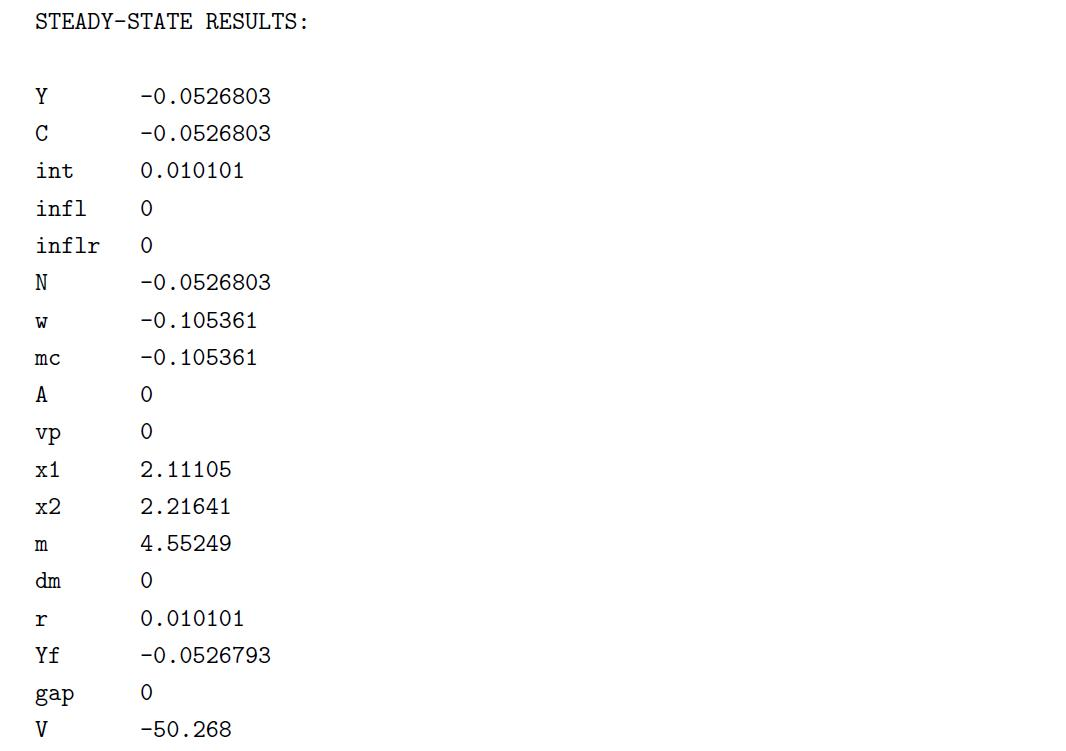
\includegraphics[width=0.8\linewidth]{FIG/SS}
		\caption{Steady State}\label{6.1}
		\centering
	\end{figure}
	
	Below are the moments, including the expected values of the variables in Figure 6.2:
	\begin{figure}[htbp!]
		\centering
		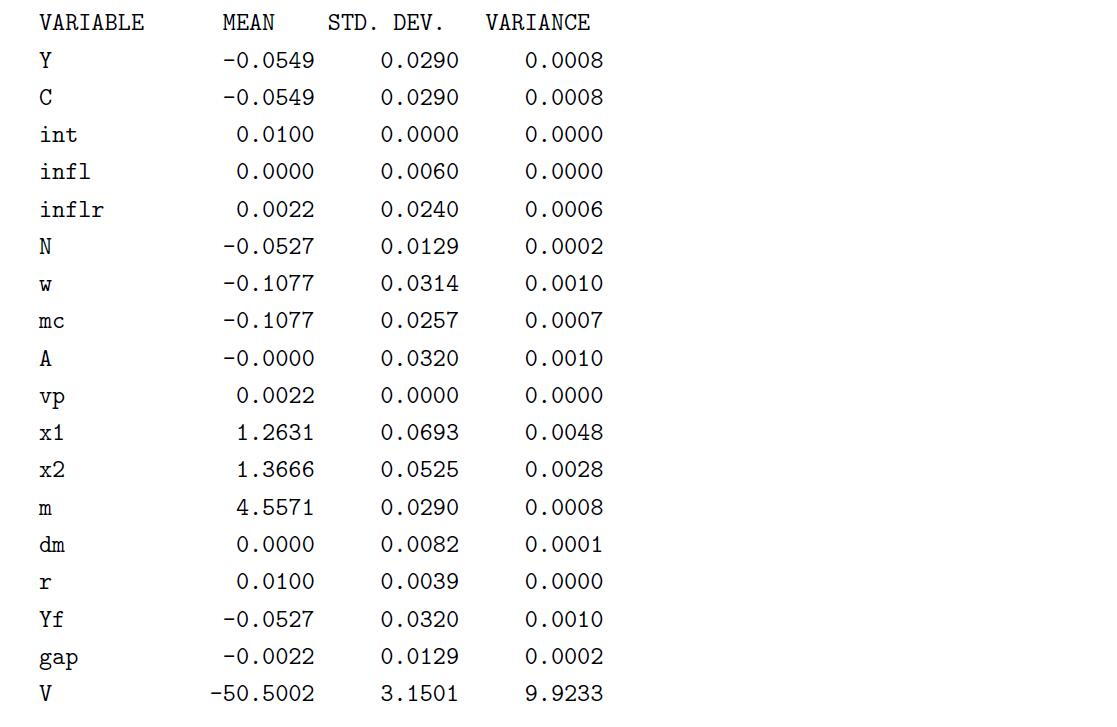
\includegraphics[width=0.8\linewidth]{FIG/moment}
		\caption{Moments}\label{6.2}
		\centering
	\end{figure}
	
	We observe here that the mean / expected value of welfare is lower (-50.5002) than steady state/welfare (-50.268). The reason why average welfare is lower than steady state welfare is because agents don't like volatility because of concavity in preferences. In a first order approximation this wouldn't show up, but in the second order approximation it does.
	
	We can then solve the model under an alternative monetary policy rule. For example, suppose that we have a money growth rule, but we set the standard deviations of monetary shocks to 0. This in effect means that the money supply would be constant. Below are the steady state values and expected values in Figure 6.3:
	
	\begin{figure}[htbp!]
		\centering
		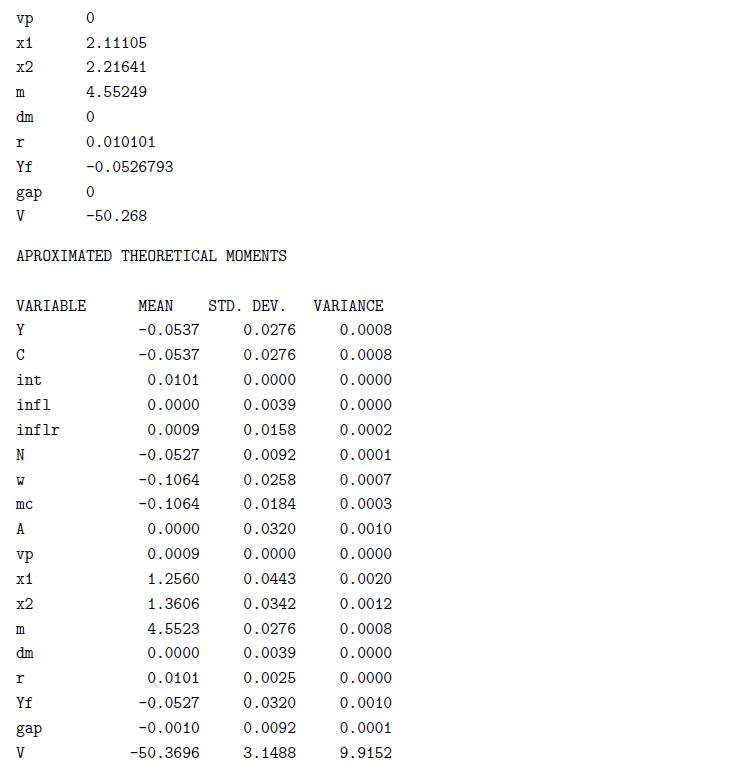
\includegraphics[width=0.8\linewidth]{FIG/alternativeSS}
		\caption{Steady State}\label{6.3}
		\centering
	\end{figure}
	
	Getting rid of the shock to the money growth rate doesn't affect the steady state value of welfare, but it does increase the mean value of welfare (-50.3696 vs. -50.5002).
	
	\subsection{Consumption Equivalent}
	
	The units of welfare are not particularly interpretable, so we often want to express the differences in "consumption equivalent" units. The thought experiment is to say "How much consumption would one be willing to give up (each period) under one policy to have the same welfare as under a different policy." It is arbitrary which policy one takes to be the "baseline"--- here I'm going to assume it's the policy with no monetary shock.
	
	Let $\lambda$ denote the fraction of consumption one would be willing to give up in each period in one economy, call this economy 0. With log utility over consumption, we have:
	
	$$E(V_t^0(\lambda))=E\left[ln(C_t(1+\lambda))-\theta\frac{N_t^{1+\xi}}{1+\xi}+\beta E_tV_{t+1}^0(\lambda)\right]$$
	
	Since the $\lambda$ shows up every period and is deterministic, this reduces to:
	
	$$E(V_t^0(\lambda))=\frac{1}{1-\beta}ln(1+\lambda)+E\left[ln(C_t)-\theta\frac{N_t^{1+\xi}}{1+\xi}+\beta E_tV_{t+1}^0(\lambda)\right]$$
	
	The term in brackets is just:
	
	$$E(V_t^0(\lambda))=\frac{1}{1-\beta}ln(1+\lambda)+E(V_t^0)$$
	
	Then we want to find the $\lambda$  that equates this with expected welfare in the alternative economy, call it economy 1. We have:
	
	$$E(V_t^0(\lambda))=E(V_t^1)$$
	
	or
	
	$$\frac{1}{1-\beta}ln(1+\lambda)+E(V_t^0)=E(V_t^1)$$
	
	Solving for $\lambda$:
	
	$$\lambda=e^{(1-\beta)(E(V_t^1)-E(V_t^0))}-1$$
	
	If I take the baseline economy 0 to have higher welfare, then the term inside the exp is negative, which means $\lambda< 0$. This makes sense { you would be willing to give up consumption in the high welfare economy to have the same welfare as another economy governed by a policy resulting in lower welfare. Using the differences in expected welfare for the two economies in question here, and a value of $\beta = 0.99$, I get a value of $\lambda = -0.0013$. This means that an agent would be willing
		to forfeit about 0.1 percent of consumption each period in the economy with no monetary shocks to avoid going to the economy with monetary shocks. This number may not seem large but we
		typically find pretty small welfare differences under different macro policies, so it's not abnormally low.
		
		I solved the model assuming zero trend inflation. Suppose I solve the model where steady state inflation is instead set to 0.005 (approximately 2 percent at an annualized frequency). Below are the steady states and the means in Figure 6.4 and 6.5:
		
		\begin{figure}[htbp!]
			\centering
			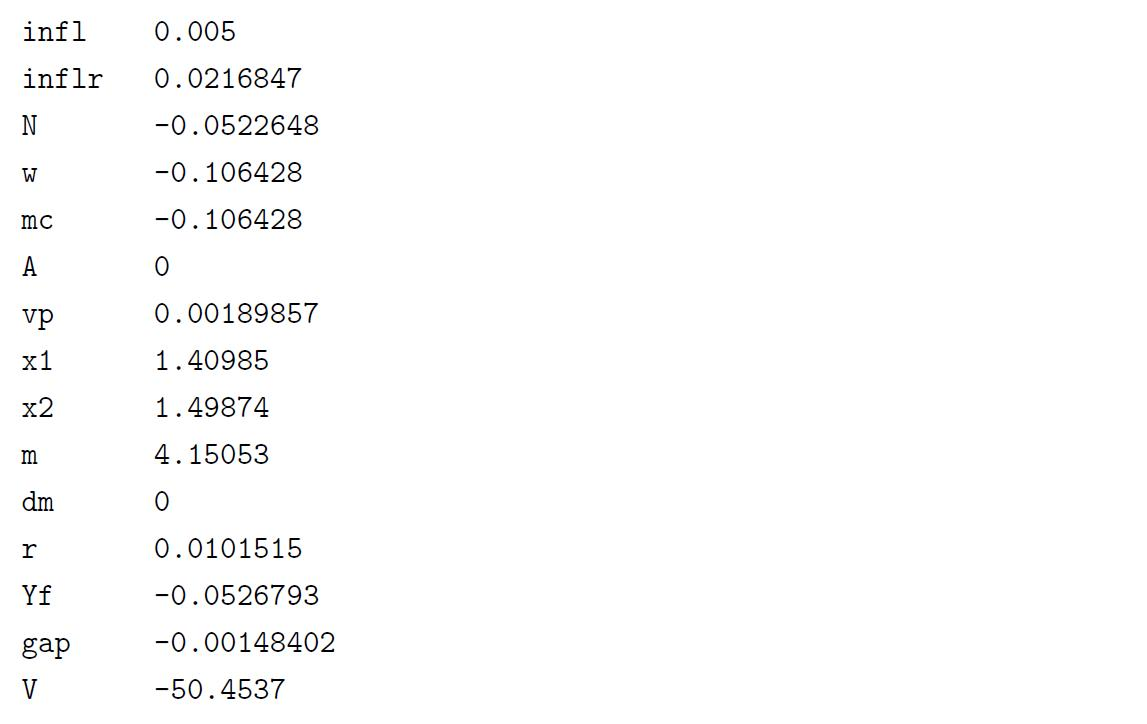
\includegraphics[width=0.8\linewidth]{FIG/SS1}
			\caption{SS}\label{6.4}
			\centering
		\end{figure}
		
		\begin{figure}[htbp!]
			\centering
			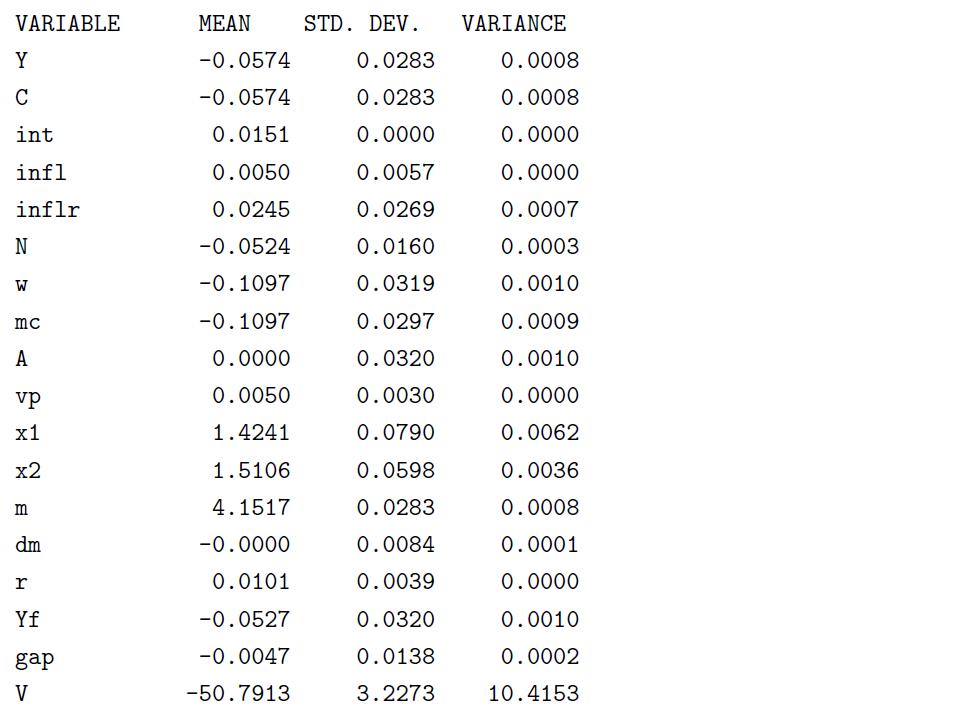
\includegraphics[width=0.8\linewidth]{FIG/moment1}
			\caption{Moments}\label{6.5}
			\centering
		\end{figure}
		
		Unlike the standard deviation of the monetary policy shock, the level of trend inflation does affect the steady state { we can see that steady state welfare is lower with higher trend inflation (-50.4537 vs. -50.268). We also see that expected welfare is lower, at -50.7913 (compared to -50.5002). We could calculate consumption equivalent welfare differences based both on steady state welfare or expected welfare. Based on steady states, we would get $\lambda = -0.0019$; based on the means, we would get $\lambda = -0.0029$.
			
			Hence, we observe that the welfare loss based on means is higher than the welfare loss based on the steady state. This is because trend inflation does two things: first, it distorts the steady state by effectively increasing the steady state markup and increasing steady state price dispersion. But it also interacts with the shocks to have a bigger effect on means: with positive trend inflation, price dispersion is first order, which makes stochastic shocks more costly.
			
	\chapter{Notes on DSGE with Learning}
	\section{Introduction}
	
	This note works through \textcolor{blue}{Winkler (2019, JME): "The role of learning for asset prices and business cycles"}. In the model, the implications of learning-based asset pricing are examined in a business cycle model with financial frictions. Agents learn about stock prices while firms face credit constraints that depend partly on their market value. Expectations are constrained to remain model- consistent conditional on a subjective belief for stock prices. The combination of financial frictions and learning amplifies shocks through a two-sided feedback mechanism between asset prices and real activity.
	
	Winkler used an otherwise standard business cycle model with two important ingredients. First, firms’ access to credit is constrained and depends on their market value. Second, agents do not have rational expectations, but are instead updating a subjective belief system about stock prices, which gives rise to extrapolation bias.
	
	In addition to these features, the model is a sticky price and wage NK with adjustment costs.It is populated by two types of households---lenders and investors. Firms are at the heart of the model and combine capital and labor into intermediate goods subject to a borrowing constraint. In addition, the model contains nominal rigidities and investment adjustment costs. Adjustment costs are introduced via capital good producers that operate competitively in
	5 input and output markets, producing capital goods using final consumption goods.Nominal rigidities are introduced via wholesale and retail firms and labor agencies.
	
	\section{The Model}
	\subsection{Households}
	\subsubsection{Lenders}
	Lending households consume final goods and supply labor. They are risk-averse, trade debt claims on intermediate goods producers and receive interest from them.
	The representative Lending Households maximize the expected present discounted value of utility:
	
	\begin{equation*}
		\underbrace{max}_{C_t,L_t,B_{j,t},B_t^g}~\mathit{E}^{\mathcal{P}} \sum_{t=0}^{\infty}\beta^t\left(\frac{C_{t}^{1-\theta}}{1-\theta}-\eta \frac{L_{t}^{1+\phi}}{1+\phi}\right)
	\end{equation*}
	
	The budget constrain of the household is
	\begin{equation*}
		C_t=w_tL_t+B_t^g-\frac{1+i_{t-1}}{\pi_t}B_{t-1}^g+\int_0^1(B_{j,t}-R_{j,t-1}B_{j,t-1})dj+\Pi_t
	\end{equation*}
	
	They consume an amount $C_t$ of a homogeneous final consumption good and supply an amount $L_t$ of labor at the real wage rate $w _t$ . $B^ g_ t$ are real quantities of nominal one-period government bonds (in zero net supply) that pay a nominal interest rate $i_ t$ , and $\pi_t=\frac{P_t}{P_{t-1}}$ is the rate of inflation. They also lend funds $B_{ jt}$ to intermediate goods producers indexed by $j \in [0, 1] $at the real interest rate $R _{jt}$ . These loans are the outcome of a contracting problem described later on. As in \textcolor{blue}{Bernanke et al. (1999)} , lending households do not own firm equity\footnote{Effectively, this leads to segmentation between bond and equity markets. From an asset pricing perspective, this assumption is somewhat unsatisfying. But from a business cycle perspective, it helps the model fit the data,If households held equity in this model, 
		fluctuations in beliefs under learning would introduce strong wealth effects: Agents that are optimistic about future stock returns have higher expected financial wealth and therefore work less and reduce their savings, which can lead to a counterfactually low rise or even a fall in investment and hours worked during expansions. Here, household wealth effects from changes in beliefs are present as well, but are more muted because they operate only through changes in expected labor income rather than expected financial wealth. So these wealth effects make it difficult to replicate the cyclicality of investment and labor in the data. A similar problem is known in the news shock literature ( \textcolor{blue}{Beaudry and Portier, 2007} ).}. $\Pi_t$ represents lump-sum profits received from price- and wage-setting firms and capital goods producers. 
	
	
	Household face an intertemporal problem, they find the value of consumption $C_t$, hours worked $L_t$,  real governmental bonds $B_{t}^g$ and real lending funds $B_{j,t}$, which delivers the highest value of utility. 
	
	A Lagrangian is
	\begin{equation*}
		\begin{aligned}
			\mathcal{L}=\mathit{E}^{\mathcal{P}} \sum_{t=0}^{\infty}\beta^t\biggm\{&\frac{C_{t}^{1-\theta}}{1-\theta}-\eta \frac{L_{t}^{1+\phi}}{1+\phi}+\lambda_t\bigg[w_tL_t+B_t^g-\frac{1+i_{t-1}}{\pi_t}B_{t-1}^g\\
			&+\int_0^1(B_{j,t}-R_{j,t-1}B_{j,t-1})dj+\Pi_t-C_t\bigg]\biggm\}
		\end{aligned}
	\end{equation*}
	
	
	The first-order conditions of households are standard. 
	\begin{equation}
		\eta L_t^{\phi}=C_t^{-\theta}w_t
	\end{equation}
	
	\begin{equation}
		\Lambda_{t,t+1}=\beta\mathit{E}^{\mathcal{P}}\frac{\lambda_{t+1}}{\lambda_t}
	\end{equation}
	
	\begin{equation}
		1=\mathit{E}^{\mathcal{P}}\Lambda_{t,t+1}\frac{1+i_t}{\pi_{t+1}}
	\end{equation}
	
	\begin{equation}
		1=\mathit{E}^{\mathcal{P}}\Lambda_{t,t+1}R_{j,t}
	\end{equation}
	
	Where $\lambda_t$ is Lagrangian multiplier.(7.1) is a standard labor supply condition, and (7.3)-(7.4) is the standard Euler equation for bonds.In particular, the stochastic discount factor of the lending household is given by (7.2) $\Lambda_{t,t+1}$. Expectations are evaluated under the probability measure $\mathcal{P}$, which does not necessarily coincide with rational expectations.
	
	\subsubsection{Investors}
	Firm owners, this is investing households only consume final goods. Investing households differ from lending households in their capacity to own intermediate firms. They are risk-neutral and trade equity claims on firms indexed by $j \in [0, 1]$ and receive dividends from them. As described above, if a firm exits, it pays out its net worth $N_{j,t}$ as a terminal dividend. Otherwise it pays a regular dividend of $D_{j,t}=\zeta E_{j,t}$,where $E_{j,t}$ is firm's earnings, this is the number $\zeta$ therefor represents the dividend payout ratio for continuing firms. Denote the subset of firms alive at the end of period t by $\varGamma_t \subset [0, 1]$. A firm owner’s/investing households utility maximization problem is:
	\begin{equation*}
		\underbrace{max}_{C_t^f,S_{j,t}}~\mathit{E}^{\mathcal{P}} \sum_{t=0}^{\infty}\beta^tC_{t}^f
	\end{equation*}
	
	The budget constrain of the household is
	\begin{equation*}
		C_t^f+\int_{j \in \varGamma_t} P_{j,t}S_{j,t}dj=\int_jS_{j,t-1}(P_{j,t}+D_{j,t})dj+\int_{j \in \varGamma_{t-1}/\varGamma_t} S_{j,t-1}N_{j,t}dj
	\end{equation*}
	
	Where $C_t^f$ is a consumption of investing households; $S_{j,t}$ is holding share of firms j equity;  $D_{j,t}$ is a dividend. $P_{j,t}$ is a stock price of firm j. The first term on the right-hand side of the budget constraint deals with continuing firms while the second term deals with exiting firms.
	
	Investors do not trade debt claims. In addition, investors face upper and lower bounds on traded stock holdings. The only reason for this assumption is to render demand for stocks finite under arbitrary beliefs. In equilibrium, the bounds are never binding.
	
	\begin{equation}
		S_{j,t} \in [0, \hat{S}]
	\end{equation}
	where $\hat{S}>1$.
	
	A Lagrangian is
	\begin{equation*}
		\mathcal{L}=\underbrace{max}_{S_{j,t}}~\mathit{E}^{\mathcal{P}} \sum_{t=0}^{\infty}\beta^t\bigg(\int_jS_{j,t-1}(P_{j,t}+D_{j,t})dj+\int_{j \in \varGamma_{t-1}/\varGamma_t} S_{j,t-1}N_{j,t}dj-\int_{j \in \varGamma_t} P_{j,t}S_{j,t}dj\bigg)
	\end{equation*}
	When $\frac{d\mathcal{L}}{dS_{j,t}}=0$, we get
	\begin{equation*}
		P_{j,t}=\beta\mathit{E}^{\mathcal{P}}\big[(P_{j,t+1}+\zeta E_{j,t+1}){\mathbf{1}_{j\in \varGamma_{t+1}}+N_{j,t+1}\mathbf{1}_{j\in \varGamma_t/\varGamma_{t+1}}\big]}
		\end{equation*}
		where $\mathbf{1}_{j\in \varGamma_{t+1}}$ is a indicator function indicating continuing firm at t+1. The term on the left-hand side of the optimal condition is marginal cost of holding share while The first term on the right-hand side is marginal revenue of next period with continuing firms, the second term is marginal revenue of next period with exiting firms.
		
		
		The first-order condition of an investor is:
		\begin{equation}
			\left.
			\begin{array}{lr}
				S_{j,t}=0, ~if~ P_{j,t}>&  \\
				S_{j,t}\in [0, \hat{S}],~ if~ P_{j,t}=\\
				S_{j,t}=0, ~if~ P_{j,t}< &  
			\end{array}
			\right\}=\beta\mathit{E}^{\mathcal{P}}\big[(P_{j,t+1}+\zeta E_{j,t+1}){\mathbf{1}_{j\in \varGamma_{t+1}}+N_{j,t+1}\mathbf{1}_{j\in \varGamma_t/\varGamma_{t+1}}\big]}
			\end{equation}
			
			
			
			\subsection{Firms}
			
			The production firms are split into four types: intermediate firms, wholesalers, retailers and capital producer. Intermediate firms produce homogeneous intermediate good. These intermediate firms produce output only using labor and subject to an aggregate productive shock. Then Wholesalers (indexed by $i \in [0, 1]$) transform the homogeneous intermediate good into differentiated varieties using a one-for-one technology. The retailers package different types of goods which are imperfect substitutes (at the origin of the monopolistic competition) to the composite final good in a CES technology. Because of imperfect substitutes of the wholesale goods in final production process, these wholesale firms have the pricing power. They are no freely able to adjust prices each period, but in Calvo's pricing.
			
			\subsubsection{Retail Firm}
			
			Retailers transform wholesale varieties into the final consumption good according to a standard Dixit-Stiglitz aggregation technology:
			
			\begin{equation}
				Y_t=\left(\int_0^1Y_t(i)^{\frac{\sigma-1}{\sigma}}dj \right)^{\frac{\sigma}{\sigma-1}}
			\end{equation}
			
			Following the profit maximization of the final good firm, we find the wholesale demand function for each variety j is:
			
			\begin{equation}
				Y_t(i)=\left(\frac{P_{i,t}}{P_t}\right)^{-\sigma}Y_t
			\end{equation}
			
			where $P_{i,t}$ is the price of variety i, $P_t$ is the general (aggregate) price level:
			
			\begin{equation}
				P_t=\left(\int_0^1P_{i,t}^{1-\sigma}dj\right)^{\frac{1}{1-\sigma}}
			\end{equation}
			
			\subsubsection{wholesale Firms}
			The Wholesalers (indexed by $i \in [0, 1]$) transform the homogeneous intermediate good into differentiated varieties using a one-for-one technology.
			\begin{equation}
				Y_{i,t}=Y_{j,t}
			\end{equation}
			Each wholesaler enjoys market power in her output market, and sets a nominal price $P_{i,t}$ . A standard Calvo friction prevents the wholesaler from adjusting her price with probability $\kappa$. The wholesaler solves the following optimization:
			\begin{equation*}
				\underbrace{max}_{P_{i,t}}\sum_{s=0}^{\infty}\bigg(\prod_{\tau=1}^{s}\kappa \Lambda_{t+1}\bigg)\biggl\{\bigg[(1+\tau)P_{i,{t+s}}-q_{t+s}P_{t+s}\bigg]Y_{i,t+s}-T_{t+s}\biggr\}
			\end{equation*}
			Subject to the wholesale demand function for each variety j is:
			
			\begin{equation*}
				Y_t(i)=\left(\frac{P_{i,t}}{P_t}\right)^{-\sigma}Y_t
			\end{equation*}
			I assume that the government sets subsidies such that $\tau =\frac{1}{1-\sigma}$ so that the steady-state markup over marginal cost is zero, and levies a lump-sum tax $T_{t}$ on wholesalers to finance the subsidy. Since all wholesalers that can re-optimize at t are identical, they all choose the
			same price $P_{i,t} = P_t^\star$. The optimal price decision is
			\begin{equation}
				\pi_t^\star=\frac{1}{1+\tau}\frac{\sigma}{\sigma-1}\frac{X_{1,t}}{X_{2,t}}
			\end{equation}
			where $\pi_t^\star=\frac{P_{i,t}}{P_t}$,and
			\begin{equation}
				X_{1,t}=q_t+\kappa \mathit{E}^{\mathcal{P}}\Lambda_{t+1}\frac{Y_{t+1}}{Y_t}\pi_{t+1}^{\sigma}
			\end{equation}
			
			\begin{equation}
				X_{2,t}=1+\kappa \mathit{E}^{\mathcal{P}}\Lambda_{t+1}\frac{Y_{t+1}}{Y_t}\pi_{t+1}^{\sigma-1}
			\end{equation}
			where $\pi_t=\frac{P_t}{P_{t-1}}$, and form (7.9) the reset price are linked through the price aggregation equation which can be written as
			\begin{equation}
				1=(1-\kappa)(\pi_t^\star)^{1-\sigma}+\kappa \pi_t^{\sigma-1}
			\end{equation}
			
			and the Tak-Yun distortion term is
			\begin{equation}
				\Delta_t=(1-\kappa)\bigg(\pi_t^\star\bigg)^{\sigma}+\kappa \pi_t^\sigma \Delta_{t-1}
			\end{equation}
			This term $\Delta_t>1$ is the wedge due to price distortions between the amount of wholesale goods produced and the amount of the final good consumed. The amount of nal goods available for consumption and investment is
			\begin{equation}
				Y_t\Delta_t=\int_{0}^{1}Y_{i,t}di=\int_{0}^{1}Y_{j,t}dj
			\end{equation}
			
			
			\subsubsection{Intermediate Goods Firms}
			
			The production of intermediate goods is carried out by a continuum of firms, indexed $j \in [0, 1]$.Firm j enters period t with capital $K_{j,t-1}$ and a stock of debt $B_{j,t-1}$ which needs to be repaid at the gross real interest rate $R_{j,t-1}$. First, capital is combined with labor $L_{j,t}$ to produce output:
			
			\begin{equation}
				Y_{j,t}=K_{j,t}^{\alpha}\bigg(A_tL_{j,t}\bigg)^{1-\alpha}
			\end{equation}
			
			where $Y_{j,t}$ is the intermediate goods, $A_t$ is a common productive shock following AR(1) process:
			
			\begin{equation}
				lnA_t=(1-\rho_a)ln\hat{A}+\rho_a lnA_{t-1}+\epsilon_{a,t}
			\end{equation}
			
			Labor is a CES combination of differentiated labor services with elasticity of substitution $\sigma_w$, but the firm's problem can be treated as if the labor index was acquired in a competitive market at the real wage index $w_t$. Output is sold competitively to final good producers at price $q_t$. The capital stock depreciates at rate $\delta$. This depreciated capital can be traded by the firm at the price $Q_t$.
			
			The firm's net worth is the difference between the value of its assets and its outstanding debt:
			\begin{equation}
				N_{j,t} = q_tY_{j,t}-w_tL_{j,t} + Q_t (1 -\delta)K_{j,t-1} -R_{j,t-1}B_{j,t-1}:
			\end{equation}
			
			I assume that firms exit with probability $\gamma$. This probability is exogenous and independent across time and firms. As in \textcolor{blue}{Bernanke et al. (1999)}, exit prevents firms from becoming financially unconstrained. If a firm does not exit, it needs to pay out a fraction $\zeta \in (0, 1)$ of its earnings as a regular dividend.
			
			The firm's earnings :
			$$E_{j,t} = N_{j,t}-Q_tK_{j,t-1}+B_{j,t-1}$$
			
			The number $\zeta$ therefore represents the dividend payout ratio for continuing firms.\footnote{The optimal dividend payout ratio in this model would be $\zeta = 0$, as firms would always prefer to build up net worth to escape the borrowing constraint over paying out dividends. However, this would imply that aggregate dividends would be proportional to aggregate net worth, which is rather slow-moving. The resulting dividend process would not be nearly as volatile as in the data. Imposing $\zeta > 0$ allows to better match the volatility of dividends and therefore obtain better asset price properties.} The firm then decides on the new stock of debt $B_{j,t}$ and the new capital stock $K_{j,t}$, maximizing the present discounted value of dividend
			payments using the discount factor of its owners. Its balance sheet must satisfy:
			\begin{equation}
				Q_tK_{j,t} = B_{j,t} + N_{j,t} -\zeta E_{j,t}
			\end{equation}
			
			If a firm does exit, it pays out its entire net worth as a terminal dividend.
			
			In choosing their debt holdings, firms are subject to a borrowing constraint.The constraint is the solution to a particular limited commitment problem in which the outside option for the lender in the event of default depends on the market value of the firm. Effectively, it introduces a link between stock market valuations and investment.
			
			Each period, lenders (households) and borrowers (firms) meet to decide on the lending of funds. Pairings are anonymous. Contracts are incomplete because the repayment of loans cannot be made contingent. Only the size $B_{j,t}$ and the interest rate $R_{j,t}$ of the loan can be contracted in period t. Both the lender (a household) and the firm have to agree on a contract ($B_{j,t};R_{j,t}$). Moreover,there is limited commitment in the sense that at the end of the period, but before the realization of next period's shocks, firm j can always choose to enter a state of default. In this case, the value of the debt repayment must be renegotiated. If the negotiations are successful, then wealth is effectively shifted from creditors to debtors. The outside option of this renegotiation process is bankruptcy of the firm and seizure by the lender. Bankruptcy carries a cost of a fraction $1-\xi$ of the firm's capital being destroyed. The lender, a household, does not have the ability to operate the firm. It can liquidate the firm's assets, selling the remaining capital in the next period. This results in a recovery value of $\xi Q_{t+1}K_{j,t}$. With some probability $x$ (independent across time and firms), the lender receives the opportunity to "restructure" the firm if it wants. Restructuring means that, similar to Chapter 11 bankruptcy proceedings, the firm gets partial debt relief but remains operational. I assume that the lender has to sell the firm to another firm owner, retaining a fraction $\xi$ of the initial debt. In equilibrium, the recovery value in this case will be $\xi (P_{j,t} + B_{j,t})$
			and this will always be higher than the recovery value after liquidation.
			
			The optimal debt contract in this limited commitment problem takes the form of a leverage constraint with a weighted average of liquidation and market value of
			the firm:\footnote{The borrowing constraint is similar to that in \textcolor{blue}{Miao and Wang (2011)} who develop a model where $x = 1$ but where only a fraction of firms are constrained, and show that this type of borrowing constraint can lead to sunspot equilibria. Such multiple equilibria do not arise for the parameter values considered in this paper.}
			\begin{equation}
				B_{j,t} \le (1 - x) \underbrace{\mathit{E}^{\mathcal{P}}\Lambda_{t+1}{Q_{t+1}\xi K_{j,t}}}_{liquidation ~value}+x \underbrace{\xi (P_{j,t} + B_{j,t})}_{market~ value}
			\end{equation}
			
			It is worth noting that even under rational expectations, the market value of the firm $P_{j,t} + B_{j,t}$ is different from the value of its capital stock, $Q_tK_{j,t}$. Because financial frictions prevent firms from investing up to the effcient level, so that the marginal discounted revenue from capital exceeds the
			marginal cost of capital. Therefore, the market value of the firm is higher than the value of its capital stock.
			
			The borrowing constraint acts as a link between firm investment and equity valuations. It is well known that in the data, stock prices comove with investment, too (\textcolor{blue}{Barro, 1990}). This could be simply because news about investment opportunities affect stock prices and predict investment
			at the same time \textcolor{blue}{Blanchard et al. (1993)}. But the literature has documented evidence that firms' investment depends on equity valuations beyond fundamentals (e.g. \textcolor{blue}{Baker et al., 2003} for equity dependent firms; and more recently \textcolor{blue}{Hau and Lai, 2013} for firms whose shares were subjected to fire sales by distressed equity funds in the 2007-2009 financial crisis). While not the only one, the borrowing constraint developed here is one possible explanation for this dependency.\footnote{Other studies examine models in which firms' credit constraints depend on the value of their real estate rather than their equity value (\textcolor{blue}{Liu et al., 2013}). Here, too, the empirical evidence is not clear-cut. For example, \textcolor{blue}{Chakraborty et al. (2016)} argue that price increases in real estate might induce lenders to substitute commercial lending with mortgage lending, thereby tightening credit constraints.}
			
			\subsubsection{The Capital Producer}
			Adjustment costs are introduced via capital good producers that operate competitively in input and output markets, producing capital goods using final consumption goods. There is no distinction between new and used capital and depreciation takes place within intermediate firms. The maximization program of capital producers is entirely intratemporal:
			\begin{equation*}
				\underbrace{max}_{I_t}~Q_tI_t-\bigg(I_t+\frac{\psi}{2}\big(\frac{I_t}{I_{t-1}-1}\big)^2\bigg)
			\end{equation*}
			Past investment levels $I_{t-1}$ are taken as given when choosing current investment output.\footnote{This setup is simpler than the one in \textcolor{blue}{Bernanke et al. (1999)} where the price of used and new capital goods differ.}
			
			The first-order condition
			\begin{equation}
				Q_t=1+\psi\bigg(\frac{I_t}{I_{t-1}}-1\bigg)
			\end{equation}
			
			
			\subsection{Aggregation and Market Clearing Conditions}
			
	\chapter{Keynesian Growth Synthesis: fluctuation and Growth}

    This note works through Gianluca Benigno and Luca Fornaro(2017,RES):"Stagnation Traps".
	\section{Introduction}
	Since the Global Crisis, productivity growth has slowed markedly in most economies (Adler et al. 2017). Can insufficient aggregate demand lead to economic stagnation, i.e. a protracted period of high unemployment and low growth? Economists have been concerned with this question at least since the Great Depression. See Hansen (1939) for an early discussion of the relationship between aggregate demand, unemployment and technical progress. 
	
	This has caused a lively debate about the role of policy, especially monetary policy, in reviving growth (Yellen 2016, Obstfeld and Duval 2018). Through which channels does monetary policy affect productivity? How should monetary policy be conducted in an economy when productivity growth is low? These questions are at the forefront of the monetary policy debate. Existing research offers little guidance to policymakers who want to understand the interactions between economic fluctuations, growth, and stabilisation policies. 
	
	Macroeconomic research has traditionally separated between its two main strands into two paradigms:
	
	\begin{itemize}
		\item Research on business cycles has focused on fluctuations around an exogenous and stable growth path.
		\item Research on endogenous growth has studied the determinants of trend growth, largely abstracting from business cycle fluctuations.
	\end{itemize}

	In sum, the macroeconomic literature offers little guidance to policymakers seeking to understand the interactions between economic fluctuations, growth, and stabilisation policies.
	
	In Benigno and Fornaro(2017,RES)' work,  they proposed a 'Keynesian growth framework' that would be able to reconcile these two paradigms. Their theory brings together the Keynesian insight that unemployment might arise from weak aggregate demand, with the notion, developed by the endogenous growth literature, that productivity growth is the result of investment in innovation by profit-maximising firms.
	
	In the model, there are two types of agents: firms and households. Firms' investment in innovation endogenously determines the growth rate of productivity and potential output of our economy. Households supply labour, consume, and participate in financial markets. Nominal wages are partially rigid, as is traditional in Keynesian analyses. This friction implies that unemployment due to weak aggregate demand is possible, and that monetary policy can affect the real economy.
	
	There are differences from traditional models. In the Keynesian growth framework business cycle fluctuations can have an impact on investment in innovation and productivity growth, and recessions might lead to permanent deviations from the pre-recession trend. Moreover, monetary policy can affect firms’ investment and productivity growth. The framework therefore allows a rigorous analysis of the interactions between economic fluctuations, productivity growth, and macroeconomic policies.
	
	In the Keynesian growth model, aggregate demand and productivity growth are tightly related by a three-way interaction.
	
	\begin{itemize}
		\item \textbf{Healthy productivity growth sustains aggregate demand and helps monetary policy to stabilise the economy.} In our framework household demand for consumption depends on expectations of future income, just as in standard macroeconomic models. For example, a slowdown in the growth rate of potential output is associated with lower future income and a reduction in current aggregate demand.1 In turn, when aggregate demand is weak it is more likely that monetary policy will eventually be constrained by the zero lower bound, preventing the central bank from stabilising the economy. Hence, healthy productivity growth plays a key role in sustaining aggregate demand and facilitating economic stabilisation through monetary policy.
		\item \textbf{Robust demand fosters productivity growth.} In our framework firms invest in innovation to gain a monopoly position, just as in standard models of vertical innovation (Aghion and Howitt 1992), and so their investment in innovation is positively related to profits.2 Through this channel, a slowdown in aggregate demand, leading to a fall in profits, also reduces firms’ investment in productivity-enhancing activities. This effect implies that maintaining the economy at full employment creates an environment favourable to firms’ investment and productivity growth. 
		
		Hence, our model suggests that healthy growth, robust aggregate demand, and resilience of the economy to business cycle shocks may be complementary. This suggests there are synergies between stabilisation policies and supply-side policies. On one hand, effective aggregate demand management is necessary to foster firm investment and productivity growth. On the other hand, pro-growth supply-side policies stimulate aggregate demand, and reduce the chance that monetary policy will be constrained by the zero lower bound.
		
		Turning to monetary policy, the Keynesian growth framework suggests that to stimulate productivity growth, the central bank should ensure that the economy operates at full employment. In fact, it is precisely when the economy operates at capacity that the incentives to invest in productivity-enhancing activities are highest. Empirical evidence recently provided by Moran and Queralto (2017), who found that monetary policy expansions led to increases in R\&D investment and productivity growth, supports this conclusion.
		\item \textbf{the Keynesian growth model shows that interaction between aggregate demand and productivity growth may create fluctuations driven by animal spirits.} Indeed, in our model pessimistic expectations about future growth can give rise to stagnation traps (protracted episodes of weak growth and high unemployment).
		
		What causes a stagnation trap? Consider a case in which agents suddenly turn pessimistic about future growth. Anticipating a fall in future income, they cut their aggregate demand. The drop in aggregate demand may be strong enough to push the policy rate against the zero lower bound, at which point conventional monetary policy loses its traction. The economy experiences a recession driven by lack of demand. This recession negatively affects firms' profits and their investment. Low investment translates into weak productivity growth, validating the initial low-growth expectations.
		
		Through this mechanism, pessimistic expectations can generate a long-lasting liquidity trap with involuntary unemployment and stagnation.3 This can last as long as agents remain pessimistic or until a successful policy intervention is implemented. Hence, in our model, a wave of pessimism about future productivity growth can generate an episode of secular stagnation.
		
	\end{itemize}	

	
	
	
	\section{The Baseline Model}
	
	The economy is inhabited by households, firms, and by a central bank that sets monetary policy.

	\subsection{Household}
	
	There is a continuum of households of measure unity. They can choose consumption, $C_t$, labor, $L_t$, bonds, $b_{t+1}$. The real return on bonds is $1+i_t$, the nominal wage is $W_t$, $d_t$are profits from ownership of firms.
	
	The household's problem is:
	
	$$
	\begin{aligned}
		&\max _{\left\{C_{t}, L_{t}, b_{t+1}\right\}_{t=0}} \mathbb{E}_{0} \sum_{t=0}^{\infty} \beta^{t}\left(\frac{C_{t}^{1-\sigma}-1}{1-\sigma}\right) \\
		&\text { s.t. } P_tC_{t}+\frac{b_{t+1}}{1+i_t}=W_{t} L_{t}+b_t+d_{t},
	\end{aligned}
	$$
	
	where is $P_t$ is the nominal price of the final good.
	
	We form a Lagrangian :
	
	$$\begin{aligned}\mathcal{L}= \mathbb{E}_{0}\left\{\sum _ { t = 0 } ^ { \infty } \beta ^ { t } \left[\left(\frac{C_{t}^{1-\sigma}-1}{1-\sigma}\right)-\lambda_{t}\left(P_tC_{t}+\frac{b_{t+1}}{1+i_t}-W_{t} L_{t}-b_t-d_{t}\right)\right]\right\}\end{aligned}$$
	
	The FOCs are 
	
	\begin{equation}
		C_t^{-\sigma} = \lambda_t P_t
	\end{equation}
	
	\begin{equation}
		\frac{\lambda_t}{1+i_t} = E_t \lambda_{t+1}
	\end{equation}
	
	\subsection{Firms}
	
	\subsubsection{Final goods firms}
	
	The final good is produced by competitive firms using labour and a continuum of measure one of intermediate inputs $x_{j,t}$, indexed by $j \in [0,1]$ . Denoting by $Y_t$ the output of final good, the production function is:
	
	\begin{equation}
		Y_{t}=L_{t}^{1-\alpha} \int_{0}^{1} A_{j t}^{1-\alpha} x_{j t}^{\alpha} d j
	\end{equation}
	
	where $0<\alpha<1$, and $A_{j,t}$ is the productivity, or quality, of input $j$. More precisely, for every good j, $A_{j,t}$ represents the highest quality available. In principle, firms could produce using a lower quality of good j. However, as in Aghion and Howitt (1992) and Grossman and Helpman (1991), the structure of the economy is such that in equilibrium only the highest quality version of each good is used in production.
	
	Given $P_{j,t}$ is the nominal price of intermediate input j. Due to perfect competition, firms in the final good sector do not make any profit in equilibrium, this is, the profits are zero, $\Pi_t = P_t Y_t - W_t L_t - P_{j,t} x_{j,t}=0$.
	
	Plugging (8.3) in the profits function, we can get the FOCs:
	
	\begin{equation}
		W_t = P_t (1-\alpha)L_{t}^{-\alpha} \int_{0}^{1} A_{j t}^{1-\alpha} x_{j t}^{\alpha} d j
	\end{equation}
		
		\begin{equation}
		P_{j,t} = P_t \alpha L_{t}^{1-\alpha} A_{j t}^{1-\alpha} x_{j t}^{\alpha-1}
	\end{equation}
		
	\subsubsection{Intermediate Goods Firms}
	
	In every industry j producers compete as price-setting oligopolists. One unit of final output is needed to manufacture one unit of intermediate good, regardless of quality, and hence every producer faces the same marginal cost $P_t$ . The assumptions about the innovation process will ensure that in every industry there is a single leader able to produce good j of quality $A_{j,t}$ , and a fringe of competitors which are able to produce a version of good j of quality $\frac{A_{j,t}}{\gamma}$ . The parameterγ $\gamma>1$ captures the distance in quality between the leader and the followers.
	
	(1) In absence of the threat of entry from the fringe of competitors, the profits for the leader is :
	
	$$\Pi_{L,j,t} = P_{L,j,t} x_{j,t} - P_t Y_t$$
	
	Plugging (8.3) and (8.5), we can get:
	
	\begin{equation}
		P_{L,j,t} = \frac{1}{\alpha} P_t
	\end{equation}
	
	(2) Without losing the market to its competitors, the profits for the followers is:
	
		$$\Pi_{F,j,t} = P_{F,j,t} x_{j,t} - P_t Y_t$$
	
	Because of  quality $\frac{A_{j,t}}{\gamma}$ of the followers' goods, plugging it in (8.5), we have:
	
		\begin{equation}
		P_{F,j,t} = \gamma^{1-\alpha}P_t
	\end{equation}
	
	So $P_{F,j,t}$ is the highest markup that the leader can charge without losing the market to its competitors, this is $P_{L,j,t}  \le \gamma^{1-\alpha}P_t$. Given this market structure, it is optimal for the leader to capture the whole market for good j by charging the price:
	
	\begin{equation}
		P_{j,t} = \xi P_t, ~~ \xi = min( \gamma^{1-\alpha}, \frac{1}{\alpha} )
	\end{equation}
	
	Where $\xi$ is a constant markup that the leader charges.
	
	Equations (8.5) and (8.8) imply that the quantity produced of a generic intermediate good j is:
	
	\begin{equation}
		x_{j,t} = \left(\frac{\alpha}{\xi}\right)^{\frac{1}{1-\alpha}}A_{j,t}L_t
	\end{equation}
	
	Combining equations (8.3) and (8.9) gives:
	
	\begin{equation}
		Y_t = \left(\frac{\alpha}{\xi}\right)^{\frac{\alpha}{1-\alpha}}A_{t}L_t
	\end{equation}
	
	where $A_t = \int_0^1 A_{j,t} dj$ is an index of average productivity of the intermediate inputs. Moreover, the profits earned by the leader in sector j are given by:
	
	$$\Pi_{j,t} = (P_{j,t} - P_t)x_{j,t} =\underbrace{P_t (\xi-1)(\alpha / \xi)^{1 /(1-\alpha)}}_{Price~Effect} \underbrace{A_{j,t}}_{Technology~Effect} \underbrace{L_t}_{Market~Size~Effect}$$
	
	According to this expression, a leader’s profits are increasing in the productivity of its intermediate input and on aggregate employment. The dependence of profits from aggregate employment is due to the presence of a market size effect. Intuitively, high employment is associated with high production of the final good and high demand for intermediate inputs, leading to high profits in the intermediate sector.
	
	\subsection{Research and innovation}
	
	There is a large number of entrepreneurs that can attempt to innovate upon the existing products. A successful entrepreneur researching in sector j discovers a new version of good j of quality $\gamma$ times greater than the best existing version, and becomes the leader in the production of good j. As in Aghion and Howitt (1992) and Grossman and Helpman (1991), all the research activities are conducted by entrants. Incumbents do not perform any research because the value of improving over their own product is smaller than the profits that they would earn from developing a leadership position in a second marketEntrepreneurs can freely target their research efforts at any of the continuum of intermediate goods. An entrepreneur that invests $I_{j,t}$ units of the final good to discover an improved version of product j innovates with probability:
	
	\begin{equation}
		\mu_{j t}=\min \left(\frac{\chi I_{j t}}{A_{j t}}, 1\right)
	\end{equation}
	
	where the parameter $\chi>0$ determines the productivity of research.The formulation of the innovation process follows closely chapter 7 of Barro and Sala-i Martin (2004) and Howitt and Aghion (1998). An alternative is to assume, as in Grossman and Helpman (1991), that labour is used as input into research. This alternative assumption would lead to identical results, since ultimately output in the model is fully determined by the stock of knowledge and aggregate labour. The presence of the term Ajt captures the idea that innovating upon more advanced and complex products requires a higher investment, and ensures stationarity in the growth process. Denoting $\mu_{j,t}$ the probability that an improved version of good j is discovered at time t. 
	
	We now turn to the reward from research. A successful entrepreneur obtains a patent and becomes the monopolist during the following period. For simplicity, in our baseline model we assume that the monopoly position of an innovator lasts a single period, after which the patent is allocated randomly to another entrepreneur.This assumption, which is drawn from Aghion and Howitt (2009) and Acemoglu et al. (2012), simplifies considerably the analysis. The value $V_t (\gamma A_{j,t} )$ of becoming a leader in sector j and attaining productivity $\gamma A_{j,t}$ is given by:

\begin{equation}
	V_{t}\left(\gamma A_{j t}\right)=\beta E_{t}\left[\frac{\lambda_{t+1}}{\lambda_{t}} P_{t+1} (\xi-1)(\alpha / \xi)^{1 /(1-\alpha)} \gamma A_{j t} L_{t+1}\right]
\end{equation}

$V_{t}\left(\gamma A_{j t}\right)$ is equal to the expected profits to be gained in period t+1, $P_{t+1} (\xi-1)(\alpha / \xi)^{1 /(1-\alpha)} \gamma A_{j t} L_{t+1}$, discounted using the households’ discount factor $\beta \frac{\lambda_{t+1}}{\lambda_{t}}$. Profits are discounted using the households’ discount factor because entrepreneurs finance their investment in innovation by selling equity claims on their future profits to the households. Competition for households’ funds leads entrepreneurs to maximize the value to the households of their expected profits. Hence, the expected returns from investing in research are increasing in future profits and decreasing in the cost of funds, captured by the households’ discount factor.

An entrepreneur that invests $I_{j,t}$ in research has a probability $\chi\frac{I_j,t}{A_j,t}$ of becoming a leader which carries value $V_t (\gamma A_{j,t} )$ . Hence, the expected return from this investment is $\chi \frac{I_{j,t}V_t (\gamma A_{j,t} )}{A_{j,t}} $. Since the investment costs $P_t I_{j,t}$ , the free entry condition in the research sector implies expected profits from researching cannot be positive, so that for every good j:

\begin{equation}
	P_{t} I_{j,t} \geq \frac{\chi I_{j,t}}{A_{j,t}} V_{t}\left(\gamma A_{j,t}\right)
\end{equation}

Simplifying the equation, we obtain the following expression: 

\begin{equation}
	P_{t}  \geq \frac{\chi}{A_{j,t}} V_{t}\left(\gamma A_{j,t}\right)
	\end{equation}

Combining this condition with expression (8.12) gives:

\begin{equation}
	V_{t}\left(\gamma A_{j t}\right)= \chi \beta E_{t}\left[\frac{\lambda_{t+1}}{\lambda_{t}} P_{t+1} (\xi-1)(\alpha / \xi)^{1 /(1-\alpha)} \gamma L_{t+1}\right]
\end{equation}

Notice that this condition does not depend on any variable specific to sector j, because the higher profits associated with more advanced sectors are exactly offset by the higher research costs. As is standard in the literature, we then focus on symmetric equilibria in which the probability of innovation is the same in every sector, so that $\mu_{j,t} =\chi \frac{ I_{j,t}}{A_{j,t}} = \mu_t$ for every j. We can then summarize the equilibrium in the research sector with the complementary slackness condition:

\begin{equation}
	\mu_{t}\left(\frac{P_{t}}{\chi}-\beta E_{t}\left[\frac{\lambda_{t+1}}{\lambda_{t}} P_{t+1} \gamma (\xi-1)(\alpha / \xi)^{1 /(1-\alpha)} L_{t+1}\right]\right)=0
\end{equation}

Intuitively, 

(1) either some research is conducted, so that $\mu_t >0$;

(2) free entry drives expected profits in the research sector to zero, or the expected profits from researching are negative and no research is conducted, so that $\mu_t =0$.

\subsection{Aggregation and market clearing}

The goods market clearing condition can be derived combining the households’ budget constraint with the
expression for firms’ profits:

\begin{equation}
	d_t = \underbrace{P_t Y_t-W_t L_t -\xi P_t \int_0^1 x_{j,t}dj}_{profit from final sector}+\underbrace{(\xi -1 )P_t \int_0^1 x_{j,t}dj-P_t \int_0^1I_{j,t}dj}_{profits from intermediate sector}
\end{equation}

This implies:

\begin{equation}
	Y_t - \int_0^1 x_{j,t}dj = C_t +\int_0^1I_{j,t}dj
\end{equation}
	
	Using equations (8.9) and (8.10) we can write GDP as:
	
	\begin{equation}
		Y_t - \int_0^1 x_{j,t}dj = \left(\frac{\alpha}{\xi}\right)^{\frac{\alpha}{1-\alpha}}\left(1-\frac{\alpha}{\xi}\right)A_tL_t
	\end{equation}
	
	The assumption of a unitary labour endowment implies that $L_t \le 1$. Since labour is supplied inelastically by the households, $1−L_t$ can be interpreted as the unemployment rate. For future reference, when $L_t =1 $ we say that the economy is operating at full employment, while when$L_t <1$ the economy operates below capacity.
	
    Long run growth in this economy takes place through increases in the quality of the intermediate goods, captured by increases in the productivity index $A_t$ . By the law of large numbers, a fraction μt of intermediate products is improved every period. Hence, $A_t$ evolves according to:

\begin{equation}
A_{t+1}=\mu_t \gamma A_t+(1-\mu_t )A_t ,
\end{equation}

while the (gross) rate of productivity growth is:

\begin{equation}
	g_{t+1}= \frac{A_{t+1}}{A_t}=\mu_t(\gamma -1 ) +1
\end{equation}

Recalling that $\mu_t =\chi \frac{I_{j,t}}{A_{j,t}}$ , this expression implies that higher investment in research in period t is associated with faster productivity growth between periods t and t+1. More precisely, the rate of productivity growth is determined by the ratio of investment in innovation $I_{j,t}$ over the existing stock of knowledge $A_{j,t} $. In turn, the stock of knowledge depends on all past investment in innovation, that is on the R\&D stock. Hence, there is a positive link between R\&D intensity, captured by the ratio $\frac{I_{j,t}}{A_{j,t}}$ , and future productivity growth.
	
	\subsection{Wage rigidities}
	
 Consider an economy with frictions in the adjustment of nominal wages. The presence of nominal wage rigidities plays two roles in the analysis. First, it creates the possibility of involuntary unemployment, by ensuring that nominal wages remain positive even in presence of unemployment. Secondly, it opens the door to a stabilization role for monetary policy. Indeed, as we will see, prices inherit part of wage stickiness, so that the central bank can affect the real interest rate of the economy through movements in the nominal interest rate.
	
	In the baseline model, consider the simplest possible form of nominal wage rigidities and assume that wages evolve according to:
	
	\begin{equation}
		W_t = \bar{\pi}^w W_{t-1}
	\end{equation}

Combining (8.4) and (8.9) give, 

\begin{equation}
	P_t = \frac{1}{1-\alpha}\left(\frac{\xi}{\alpha}\right)^{\frac{\alpha}{1-\alpha}}\frac{W_t}{A_t}
\end{equation}
	
Intuitively, prices are increasing in the marginal cost of firms producing the final good. An increase in wages puts upward pressure on marginal costs and leads to a rise in prices, while a rise in productivity reduces marginal costs and prices. This expression, combined with the law of motion for wages (8.22), can be used to derive an equation for price inflation:	
	
	\begin{equation}
		\pi_t = \frac{P_t}{P_{t-1}} = \frac{\bar{\pi}^w}{g_t}
	\end{equation}
	
	which implies that price inflation is increasing in wage inflation and decreasing in productivity growth.
	
	\subsection{Government}
	
	The central bank implements its monetary policy stance by setting the nominal interest rate according to the truncated interest rate rule:
	
	\begin{equation}
		1+i_t = max \left((1+\bar{i})\left(\frac{L_t}{\bar{L}}\right)^\phi,1\right)
	\end{equation}
	
	Under this rule the central bank aims at stabilizing output around its potential level by cutting the interest rate in response to falls in employment.
	
	\subsection{The Full Equilibrium Conditions}
	
	There are 8 equations for 8 endogenous variables:
	
	$$
	\begin{aligned}
		X_{t} \equiv \left[C_t, i_t, \pi_t, \mu_t, L_t, A_t, g_t, W_t\right]
	\end{aligned}
	$$
	
	The 8 equations are the following:

	\begin{equation}
		\frac{1}{1+i_t} = \beta E_t \frac{C_{t+1}^{-\sigma}}{C_{t}^{-\sigma}}\frac{1}{\pi_{t+1}}
	\end{equation}
	
	\begin{equation}
		\mu_{t}\left(\frac{1}{\chi}-\beta E_{t}\left[\frac{C_{t+1}^{-\sigma}}{C_{t}^{-\sigma}} \gamma (\xi-1)(\alpha / \xi)^{1 /(1-\alpha)} L_{t+1}\right]\right)=0
	\end{equation}
	
	\begin{equation}
A_{t+1} = \mu_t\gamma A_t+(1-\gamma)A_t
	\end{equation}

	
	\begin{equation}
		g_{t+1}=\frac{A_{t+1}}{A_t}
	\end{equation}
	
		\begin{equation}
		W_t = \bar{\pi}^w W_{t-1}
	\end{equation}
	
	\begin{equation}
		\pi_t =  \frac{W_t}{W_{t-1}}\frac{1}{g_t}
	\end{equation}
	
	Using (8.11), Consider that:
	$$\int_0^1 I_{j,t}dj = \int_0^1 \frac{A_{j,t}I_{j,t}}{A_{j,t}}dj =\frac{I_{j,t}}{A_{j,t}} \int_0^1 A_{j,t}dj = \frac{\mu_t}{\chi}\int_0^1 A_{j,t}dj =A_t\frac{\mu_t}{\chi}$$
	
	Using the following:
$$
		Y_t - \int_0^1 x_{j,t}dj = C_t +\int_0^1I_{j,t}dj
		$$
	
$$
		Y_t - \int_0^1 x_{j,t}dj = \left(\frac{\alpha}{\xi}\right)^{\frac{\alpha}{1-\alpha}}\left(1-\frac{\alpha}{\xi}\right)A_tL_t
	$$
	
	We can get:
	
	\begin{equation}
		C_t =  \left(\frac{\alpha}{\xi}\right)^{\frac{\alpha}{1-\alpha}}\left(1-\frac{\alpha}{\xi}\right)A_tL_t-A_t\frac{\mu_t}{\chi}
	\end{equation}
	
	
	Monetary Policy:
	\begin{equation}
		1+i_t = max \left((1+\bar{i})\left(\frac{L_t}{\bar{L}}\right)^\phi,1\right)
		\end{equation}
	
	Define $c_t = \frac{C_t}{A_t}$, using (8.26), we have \textbf{IS curve}:
	
	\begin{equation}
			\frac{1}{1+i_t} = \beta E_t \frac{c_{t}^{-\sigma}}{c_{t+1}^{-\sigma}}g_{t+1}^{-\sigma}\frac{1}{\pi_{t+1}}
	\end{equation}

	\textbf{Monetary Policy}:
\begin{equation}
	1+i_t = max \left((1+\bar{i})\left(\frac{L_t}{\bar{L}}\right)^\phi,1\right)
\end{equation}

Using (8.27)-(8.28)

\begin{equation}
	\frac{g_{t+1}-1}{\chi(\gamma-1)}\left\{1-\beta E_t \frac{c_t^\sigma}{c_{t+1}^\sigma}g_{1+1}^{-\sigma}\chi \gamma (\xi-1)(\alpha / \xi)^{1 /(1-\alpha)} L_{t+1}\right\}=0
	\end{equation}

This equation captures the optimal investment in research by entrepreneurs. For values of profits sufficiently high so that some research is conducted in equilibrium and $g_{t+1}>1$, this equation implies a positive relationship between growth and expected future employment. Intuitively, a rise in employment, and consequently in aggregate demand, is associated with higher monopoly profits. In turn, higher expected profits induce entrepreneurs to invest more in research, leading to a positive impact on the growth rate of the economy. This is the classic market size effect emphasized by the endogenous growth literature. But higher expected growth reduces households’ desire to save, leading to an increase in the cost of funds for entrepreneurs investing in research. In fact, in the new equilibrium the rise in growth and in the cost of funds will be exactly enough to offset the impact of the rise in expected profits on the return from investing in research. This ensures that the zero profit condition on the market for research is restored.

we can get \textbf{Growth curve}:

\begin{equation}
g_{1+1}^{\sigma} = \beta E_t \frac{c_t^\sigma}{c_{t+1}^\sigma}\chi \gamma (\xi-1)(\alpha / \xi)^{1 /(1-\alpha)} L_{t+1}
\end{equation}

\textbf{Market clearing condition}:

\begin{equation}
	c_t =  \left(\frac{\alpha}{\xi}\right)^{\frac{\alpha}{1-\alpha}}\left(1-\frac{\alpha}{\xi}\right)L_t-\frac{g_{t+1}}{\chi(\gamma-1)}
\end{equation}

Using(8.30)-(8.31), we have \textbf{inflation dynamics}:

\begin{equation}
	\pi_t = \frac{\bar{\pi}^w}{g_t} 
\end{equation}

\subsection{Steady state}

In steady statam, price inflation is fixed:

\begin{equation}
	\pi = \pi_{target}
\end{equation}
 
 Using (8.39), we get :
 
 \begin{equation}
 	g = \frac{\bar{\pi}^w}{\pi}
  \end{equation}

Using (8.37), we can get:

\begin{equation}
	L=\frac{g^\sigma}{ \beta \chi \gamma (\xi-1)(\alpha / \xi)^{1 /(1-\alpha)}}
\end{equation}

Using (8.34), we get:

\begin{equation}
	i = \beta \frac{g^{-\sigma}}{\pi}
\end{equation}

	Using (8.38), we can get:
	
	\begin{equation}
			c =  \left(\frac{\alpha}{\xi}\right)^{\frac{\alpha}{1-\alpha}}\left(1-\frac{\alpha}{\xi}\right)L-\frac{g}{\chi(\gamma-1)}
	\end{equation}
	
	\section{Macroeconomic Implications}
	
	\subsection{Parameterization}
	
% Process exited with error(s)
	\begin{tabular}{|l|c|c|}
	\hline
	Name & implication & Values \\
	\hline
	\beta & 1 & 0.99 \\
	\hline
	\sigma& 1 & 2 \\
	\hline
	\gamma & 1 & 1.05 \\
	\hline
	\chi & 1 & 89.14 \\
	\hline
	\alpha & 1 & 0.5 \\
	\hline
	\pi^w & 1 & 0.98 \\
	\hline
	\phi & 1 & 1 \\
	\hline
\end{tabular}

	\subsection{Dynare codes}
	
	\begin{lstlisting}
		1	%%%%%%%%%%%%%%%%%%%%%%%%%%%%%%%%%%%%%%%%%%%%%%%%%%%%%%%%%%%%%%%%%%%%%%%%%%%
		2	Stagnation Traps by Benigno and Fornano(2017,RES)
		3	%%%%%%%%%%%%%%%%%%%%%%%%%%%%%%%%%%%%%%%%%%%%%%%%%%%%%%%%%%%%%%%%%%%%%%%%%%%
		4	
		5	% This Dynare code simulates a DSGE model of endogenous growth as in  Benigno and Fornano(2017,RES).
		6	% Dynare code by Wenddy XU, 20/10/2020
		7	
		8	close all;
		9	warning off
		10	
		11	%%
		12	%%%%%%%%%%%%%%%%%%%%%%%Endogenous Variables %%%%%%%%%%%%%%%%%%%%%%%%%%%%%%%
		13	var i pi c g l;
		14
		15 varexo e_i;
		16
		17 parameter beta sigma pi_targeta fi alfa xi chi gamma piw;
		18
		19 beta = 0.99;
		20 sigma = 2;
		21 pi_target = 0.01;
		22 fi = 1;
		23 alfa =0.5;
		24 chi = 89.14;
		25 gamma = 1.05;
		26 xi = gamma^{1-alpha};
		27 piw = 0.98;
		28
		29 model;
		30  
	\end{lstlisting}
	
	
	\section{The Extended Model}
	
	
	
	
	
	\section{Further Readings}
	
    
    
    
    \chapter{DSGE with Chaos}	
	
	\section{Introduction}
	
	\section{The Deterministic Case}
	
	
	\section{The Solution Method}
	
	
	
	\section{The Stochastic Case}
	
	
	\section{Application}
	
	
	
	
	
	\chapter{Estimation Methods of Moment}
	
	Macroeconomists have made substantial investments in Moment-Matching method during the last 10 years. One reason is that Moment methods afford researchers the chance to estimate and evaluate a wide variety of macro models that econometrics often find challenging.
	
	\section{GMM}
	
	\subsection{Theory on GMM Estimation}
	This content works through Martin M. Andreasen(2019):"A toolbox for GMM estimation of DSGE models approximated up to third order - version 2".We introduce the GMM estimator, the asymptotic distribution of this estimator, and the considered moments for our GMM estimator. For additional introduction to GMM, see for instance Hamilton (1994) and Ruge-Murcia (2007).
	
	\subsection{Implementing GMM Estimation in the Dynare}
	
	
	\section{SMM}
	
	\subsection{Theory on SMM Estimation}
	This content works through Martin M. Andreasen(2019):"A toolbox for GMM estimation of DSGE models approximated up to third order - version 2".We introduce the GMM estimator, the asymptotic distribution of this estimator, and the considered moments for our GMM estimator. For additional introduction to GMM, see for instance Hamilton (1994) and Ruge-Murcia (2007).
	
	\subsection{Implementing SMM Estimation in the Dynare}
	
	
	
	
	\section{IRF-matching}
	
	
	
	\nocite{*} 
	\printbibliography
	\appendix
	
	\chapter{FAQ of Dynare}
	
	To make sure this section is as user friendly as possible, the best is to compile what users have to say! Please let me know what your most common problem is with Dynare, how Dynare tells you about it and how you solve it. Thanks for your precious help!\textcolor{blue}{Main sources: Dynare Forum(\url{forum.dynare.org})}.
	
	\section{Model Comparison}
	
	\begin{enumerate}
		\item same data for models, same priors for models, but additional parameters for one, not for another. Then does that bias the posterior odds ratio/model comparison?\\
		\textcolor{red}{Reply: For bayesian model comparison, models don't need to be nested and there is a natural degrees of freedom correction. Hence, as long as you use the same data, having different parameters does not at all.}
		\item Based on the formula of posterior odds ratio, since same data and prior, it is enough to compare marginal densities?\\
		\textcolor{red}{Reply: That is sufficient. The prior over parameters does not matter, but the prior odds ratio over the models(see Koop(2003):Bayesian Econometrics). If you a prior assign equal probability to all models(0.5 for two models), you simply compare the marginal data densities.}
		\item From the estimation results:"Log data density" was compared using \textcolor{blue}{Modified Harmonic Mean} and "Log data density [\textcolor{blue}{Laplace approximation}]" via Laplace, right?\\
		\textcolor{red}{Reply: Both the Laplace approximation and the modified harmonic mean estimation are ways to compute the marginal data density. As computing the marginal data density involves solving a complicated integral, these two methods for trackling the issue have been proposed. In theory, they should yield identical results as they measure the same thing. In practice, both involve approximations and may yield differing results.\\
			It is hard to tell which one to prefer. Footnote of SW(2007) state:" As discussed in John Greweke(1998), the MH-based sample of the posterior distribution can be used to evaluate the marginal likelihood of the model. Following Geweke(1998), we calculate the \underline{modified harmonic mean} to evaluate the integral over the posterior sample. An alternative approximation is the \underline{Laplace approximation} around the posterior mode, which is based on a normal distribution. In our experience, the results of both approximations are very close in the case of our estimated DSGE model. This is not too surprising, given the generally close correspondence between the histograms of the posterior sample and the normal distribution around the estimated mode for the individual parameters. Given the large advantage of the Laplace approximation in terms of computational costs, we will use this approximation for comparing alternative model specifications in the next section."}
		\item The decision rule for model comparison using marginal densities is: higher = better? e.g. model A(-950), model B(-1000), then choose model A.\\
		\textcolor{red}{Reply: The marginal data density to be as high as possible. The logarithm is monotonic transformation, so we also want the log marginal densities to be as high as possible.}
		
		
		\item Do one need to make any transformation on these values first?\\
		\textcolor{red}{Reply: It is often easier to compare models using posterior mode probabilities, see Koop(2003,p4).}
		
		\item Additional shocks matter?
		\textcolor{red}{Reply: No matter. What matters is that you estimate those shocks' standard deviation. But this just another parameter. Note that: you do not need the same prior.}
		
		\item In the \textcolor{blue}{model\_comparison} command,
		\begin{itemize}
			\item \textcolor{red}{Bayes\_Ratio}~~refers to the ratio of Marginal Data Densities often called \underline{Bayes Factor}\footnote{Bayes Factor,Wikipedia,\\In statistics, the use of Bayes factors is a Bayesian alternative to classical hypothesis testing. Bayesian model comparison is a method of model selection based on Bayes factors. The aim of the Bayes factor is to quantify the support for a model over another, regardless of whether these models are correct.\\
				\textbf{Definition}\\
				The Bayes factor is a ratio of the likelihood probability of two competing hypothesis, usually a null and an alternative.\\
				The posterior probability $Pr(M|D)$ of a model M given data D is given by Bayesi theorem:
				$$Pr(M|D)=\frac{Pr(D|M)Pr(M)}{Pr(D)}$$
				The key data-dependent term $Pr(D|M)$ is a likelihood, and represents the probability that some data are produced under the assumption of this model, M; evaluating it correctly is the key to Bayesian model comparison.\\
				Given a model selection problem in which we have to choose between two models on the basis of observed data D, the probability of the two different models $M_1$ and $M_2$, parameterised by model parameter vectors $\theta_1$ and $\theta_2$ is assessed by the Bayes factor K given by
				$$K=\frac{Pr(D|M_1)}{Pr(D|M_2)}=\frac{\int Pr(\theta_1|M_1)Pr(D|\theta_1,M_1)d\theta_1}{\int Pr(\theta_2|M_2)Pr(D|\theta_2,M_2)d\theta_2}=\frac{Pr(M_1|D_1)}{Pr(M_2|D_2)}\frac{Pr(M_2)}{Pr(M_1)}$$
				When the two models are equally probable a priori, so that $Pr(M_1)=Pr(M_2)$, the Bayes factor is equal to the ratio of posterior probabilities of $M_1$ and $M_2$. If instend of the Bayes factor integral, the likelihood corresponding to the maximum likelihood estimate of the parameter for each model is used, then the test becomes a classical likelihood-ratio test. Unlike a likelihood-ratio test, this Bayesian model comparison does not depend on any single set of that is automatically, and quite naturally, includes a penalty for including too much model structure. It thus guards against overfitting. For models where an explicit version of the likelihood is not available or too costly to evaluate numerically, approximate Bayesian computation can be used for model selection in a other approaches are:
				\begin{itemize}
					\item to treat comparison as a decision problem, computing the expected value or cost of each model choice;
					\item to use minimum message length(MML).
				\end{itemize}
			}.
			\item \textcolor{red}{Posterior\_Model\_Probability}~~gives you the posterior probability of the models. It is not identical to the Posterior Odds Ratio, because the Odds Ratio gives you the relative instead of the absolute probabilities. But given that the probability must sum to 1, you can compute them.\\
			For example, if you compare two models and the Model 1 has a Posterior\_Model\_Probability of 2/3, then the other model has to have one of 1/3 and Posterior Odds Ratio is (2/3)/(1/3)=2:1.
			\item \textcolor{red}{Marginal Data Density(MDD)}~~measure fit relative to other models on the same data. Note that it is pretty meaningless on its own.
			\item \textcolor{red}{The acceptance rate}~~only tells you about efficiency of the MCMC. Note that it does not tell you about convergence.
			\item \textcolor{red}{The Geweke diagnostics} for convergence.
		\end{itemize}
		
	\end{enumerate}
	
	\section{Parameter Estimation}
	
	\begin{enumerate}
		\item Whether it is possible to perform the parameter estimation using a very small sample with annual data?\\
		\textcolor{red}{Reply: That is not ideal, but doable. The prior distribution will most probably play an important role in the case, i.e. the data will not be very informative.}
		\item The model is stochastically singular.\\
		\textcolor{red}{Reply: Either that the number of observation variables is greater than the number of shocks, or observation imply an exact linear combination(more likely). Either that or measurement errors.}
		\item Based on bayesian method, we have the formula:
		\begin{enumerate}
			\item log(posterior density)=log(likelihood)+log(prior density)
			\item combining with Dynare, then log-post(blue line) is log(posterior density) and log-lik kernel(green line) is log(likelihood).
			\item right?
		\end{enumerate}
		\textcolor{red}{Reply: Right}
		\item (1)If the mode\_check plot show that mode of log-post and log-lik kernel are identical, then we can consider this mode as the mean of proposal density for the MH algorithm. Otherwise, we have to find the mode again as long as mode of log-post and log-lik kernel are identical. Right? (2)If we can not find the truly global mode, then the MH algorithm can not converge. If  such, how to find the truly global mode?\\
		\textcolor{red}{Reply: From the Bayes theorem, we know that the posterior density is equal to the likelihood times the prior density divided by the marginal density of the data:
			$$p(\theta|y_T)=\frac{p(y_T|\theta)p(\theta)}{p(y_T)}$$
			The numerator is posterior kernel (it's not a density, because it does not integrate to 1). If you are only concerned by the inference about the parameters($\theta$), you do not need to worry the denominator, all the information about the parameters is embodied in the posterior kernel. The mode\_check option will return plots of the log of the posterior kernel and of the log likelihood as a function of one parameter, keeping the other parameters constant (equal to the estimated posterior mode). So if you has two parameters $\theta_1$ and $\theta_2$, and if your estimation of posterior mode is ($\hat{\theta}_1,\hat{\theta}_2$), you will have the plots for:
			$$f(\theta_1)==logp(y_T|\theta_1,\hat{\theta}_2)+logp(\theta_1,\hat{\theta}_2)$$
			and
			$$g(\theta_1)==logp(y_T|\theta_1,\hat{\theta}_2)$$
			with $\theta_1$ taking values around $\hat{\theta}_1$. and
			$$f(\theta_2)==logp(y_T|\hat{\theta}_1,\theta_2)+logp(\hat{\theta}_1,\theta_2)$$
			and
			$$g(\theta_2)==logp(y_T|\hat{\theta}_1,\theta_2)$$
			with $\theta_2$ taking values around $\hat{\theta}_2$. \\
			So these curves are not the full multi-dimensional log likelihood and posterior kernel, but only two-dimensional cuts through these objects. Note also that because the prior density is the difference between the two objects, the log likelihood is typically smaller equal than posterior kernel (if the log prior density is positive), i.e. the graph of the likelihood would be below the posterior density and potentially not in the picture. For that reason, the likelihood is shifted upwards to have the same maximum as the posterior kernel in order to better compare them.\\
			There is absolutely no reason to seek for an estimation where these cuts through the objects are identical. Indeed, if the prior brings some information to the inference about parameters, the curves have to be different, and in general the mode of the posterior kernel (or density) does not match the mode of the likelihood.\\
			The last statement about the importance of finding the posterior mode is wrong. The MCMC will converge even if it starts from an initial state different from the (global) posterior mode, as long as for the initial state the posterior density is strickly positive, the jumping proposal density covariance is positive definite, and that all the usual assumptions on the posterior density are sutisfied. You will typically need a lot more iterations if the initial state is in a low posterior density region, but the MCMC will eventually converge to the posterior distribution. Actually, as long as mh\_nblocks is greater than one (the default being two). Dynare does not start the MCMC from the estimated posterior mode. Rather, the initial stae of each chain is chosen randomly to be overdispersed around the estimated posterior mode (the distance to the estimated posterior mode is controlled by option mh\_init\_scale).\\
			The form of the proposal (or jumping) distribution matters more than the initial state of the chain(s) for determining the number of iterations needs to ensure convergence. It is essentially in this respect that the estimation of the posterior mode is important, because we use the inverse Hessian at the estimated mode as an approximation of the posterior covariance matrix.}
		\item In An and Schorfheide(2007) "Bayesian Analysis of DSGE model", for random-walk metropolis algorithm\footnote{As the name suggests, the random walk MH algorithm specifies the candidate generating density as a random walk:
			$$\Phi^{G+1}=\Phi^G+e$$
			where $\Sigma$ the variance of $e_t$ is set by the researcher. $\Sigma=\hat{\Omega}\times \lambda$, where $\hat{\Omega}$ is the estimated variance, $\lambda$ is the scaling factor. A higher value for $\Sigma$ could mean a lower rate of acceptances across the MH iterations (i.e. the acceptance rate is defined as the number of accepted MH draws divided by the total number of MH draws) but would mean that the algorithm explores a larger parameter space. In contrast, a lower value for $\Sigma$ would mean a larger acceptance rate with the algorithm considering a smaller number of possible parameter values. The general recommendation is to choose $\Sigma$ such that the acceptance rate is between 20\% to 40\%. We consider the choice of $\Sigma$ in detail in the examples described below.\\
			See Chib and Ramamurthy (2010), Blake and Mumtaz(2017) for a more efficient version of the basic algorithm described above.}, they chose two jump parameters:\textcolor{blue}{mh\_init\_scale=1} and \textcolor{blue}{mh\_jscale=0.3} (the rejection rate is about 45\%). So is there any general rule to choose mh\_init\_scale and mh\_jscale? In Dynare, the default value for mh\_init\_scale=2*mh\_jscale, this jump factor should be adjusted, rihgt?\\
		\textcolor{red}{Reply:
			\begin{itemize}
				\item mh\_jscale should be adjusted to give an acceptance rate of 23\%. For a multivariate normal posterior, this would be the most efficient choice to get quick convergence. For mh\_init\_scale, there is less good guidance. It should be bigger than mh\_jscale to be overdispersed, but typically not too big, 2*mh\_jscale is usually a good compromise.
				\item The target 23\% acceptance rate is at best a rule of thumb. To our knowledge, there is no proof that this would be optimal for a particular DSGE model. So We do not think that we should be obsessed by this target.
				\item The choice for the parameter mh\_init\_scale does not affect the convergence of the MCMC. It is here to ensure that the initial conditions of the chains(if mh\_b=nbloks>1) are different enough. This parameter only affects the convergence diagnostics.
				\item It works quite well in practice. Anything in the range of 20 to 30 percent should be ok!
			\end{itemize}
		}
		\item How to adjust the jump scale to have a "reasonable" acceptance ratio of between 0.2 to 0.4 suggested by the literature?\\
		\textcolor{red}{Reply: The tuning the scale parameter so that the acceptance ratio is between 0.2 to 0.4 is only a heuristic.From very simple models, we know that the acceptance rate should depend on dimension of the problem (the number of estimated parameters), and should be in this region. You can find an introduction on this in the book by Robert and Casella "Monte Carlo Statistical Methods"(Chapter 7, in particular section 7.8.4).\\
			We only know for sure that acceptance ratios close ro 0 or 1 are bad. I usually target one third. But we cannot be sure, controlling only one parameter, that the acceptance rates will be the same across chains. Normally in the end, if the chains are long enough the acceptance ratios should be similar across chains. A small acceptance rate does not mean that the MCMC is trapped in a low density region. Imagine that the current state of the MCMC rate is the posterior mode. If the jumps provided by the proposal distribution are large it is very likely that all the proposals will be rejected (resulting in a low acceptance rate).}
		\item (1)Dynare compute the RW Metropolis-Hasting acceptance ratio as R =number of accepted draws/number of proposals. Right?(2)Normally, we prefer that the acceptance ratio should not be very close to 0 or 1, an ideal ratio is around 1/3. To reach the ideal ratio, we should adjust the jump scale (in Dynare, we adjust by using mh\_jscale). Based on that, one set my jump scale with 0.3. Moreover, one set number of the MH chain with 10 and number of iteration with 200,000. So then lauching Dynare, I found that: for the first MH chain, Dynare report the RW Metropolis-Hasting(1/10) Current acceptance ratio of around 0.256. However, the RW MH(2/10) Current acceptance ratio reduces a lot to 0.129 in the second MH Chain. The acceptance ratio of 0.129 is very far from the ideal ratio of 1/3. Even though I do not change the jump scale. The jump scale is still the same as 0.3 in the first MH Chain. Why the acceptance ratio is not identical for all MH Chain with the same jump scale?\\
		\textcolor{red}{Reply:
			\begin{itemize}
				\item The understanding of the acceptance ratio is correct.
				\item This is simply impossible. You cannot tune a single parameter so that all the chains have the same acceptance ratios. The fact that the acceptance rate is significantly lower in one of the chains is a matter of chance(the initial condition of this chain may be far from the initial conditions of the other chains, and the proposals are obviously different).\\
				Frankly I would not bother about this. As long as all the acceptance ratios are strickly positive, there is no trouble.
				\item I trend to somewhat disagree with the above answer. If your acceptance rates very different, it suggests that you are not sampling from the same distribution, i.e. at least one chain does not sample from the ergodic distribution we are interested in. As the above, the difference may just be due to the initial convergence to the ergodic distribution. But this then suggests that the burnin is very large relative to the actual draw, i.e. your chain are too short. For that reason, I would be extremely careful in checking convergence (and the initial mode).\\
				Also, you might want to consider fewer, but longer chains in this case.
				\item This is most probably the problem, 200,000 is not enough. At this stage, i.e. as long as the chains did not converge to the (common) ergodic distribution, the total number of draw of 200,000 is not very pertinent, only the number of iteration per chain matters. As the above suggested that reduce the number of chains (I never use more than 5), or run the estimation with the parallel capabilities of Dynare.
			\end{itemize}
		}
		\item A common problem that plogues the estimation of DSGE models is the computation of the inverse of the Hession at the posterior mode, that is not positive definite. I am aware that the option mode\_compute=5 offers a different way of computing the Hessian, optim=\{'Hessian',2\}. This seems to work well, from what I have seen. Do other optimisers also offer similar options?\\
		\textcolor{red}{Reply:
			\begin{itemize}
				\item I believe the answer is no. However, mode\_compute=6, which is based on MCMC, provides an estimate of the posterior covariance matrix not based on the inverse of the Hessian matrix(we use MCMC draws, so it works as long as the acceptance ratio is not too close to 0). Also, it is not mandatory to estimate the posterior mode(with Hessian at the estimated mode) for running a metropolis. You can optionally use another covariance matrix for the jumping distribution.
				\item mode\_compute =5 with optim=\{'Hessian',2\} relies on the outer product of gradients and requires the use of a univariate Kalman fiter. Therefore, something similar is not avaiable for other optimizers. As the above indicated, mode\_compute=6 also differs.\\
				The reason for using the inverse Hessian at the mode is that this is the most efficient choice if the posterior would be normal. But any positive definite matrix for the proposal density will do. You could provide any arbitrary matrix via command.
				\item We use the draws of the Metropolis (run in mode\_compute=6) to estimate the posterior covariance matrix. We need to have enough variability in these draws.If all the draws were identical (or more generally if the number of parameters) the sample covariance matrix would obviously not be full rank. That's why we target, by default, an acceptance rate of 1/3 (which is the value commonly considered in the literature.\\
				The optimization routine has several steps:
				\begin{description}
					\item[1] we run a Metropolis, where we tune the scale parameter so that the acceptance rate is close to the target. In this first step the draws are not used to estimate the covariance matrix, we only continuously keep record of the vector of parameters which gives the best value for the objective. In this first step the covariance matrix if the jumping distribution is an identity matrix.
					\item[2] we run a Metropolis to estimate the covariance matrix. Again we continuously keep record of the vector of parameters which gives the best value for the objective.
					\item[3] We return to 1, with the new estimate of the posterior covariance matrix.\\
					By default, we iterate on these steps two or three times( I do not remeber, look at the reference manual). And in the last step we run a last metropolis, where we only update our estimate of the posterior mode. In this last round we decrease slowly the size of the jumps.
				\end{description}
			\end{itemize}
		}
		\item Why the Hessian found by the numerical optimisers is not positive definite?\\
		\textcolor{red}{Reply: In Dynare we do not use the Hessian matrices returned by the optimizers. For instance, mode\_compute=4, the default algorithm derived from Chris Sims code, returns a crude estimate of the Hessian that is not used by Dynare (see any presentation of the BFGS, there is nice page on wikipedia, algorithm which is close to what is done here). Instead we compute the Hessian with finite difference (expect mode\_compute=6 and mode\_compute=5 which uses a gradient the outer product approach), by calling hessian.m function.\\
			The main culprit is that the optimization routine failed in finding a (local) minimum of minus the likelihood (or posterior kernel). That's why you need to play with other optimization routine and/or the initial guesses. Another culprit, may be the noise in the objective function. In this case you have to change the length of the steps in the finite difference routine (controlled by options\_.gstep).\\
			Two additional issue are:
			\begin{itemize}
				\item the Hessian only needs to be positive definite at an interior solution. If you have a corner solution, i.e. you are at the bound of your prior parameter space, there will be a problem.
				\item if a parameter is not identified or if there is collinearity in the jacobian of the likelihood, the Hessian will also be non-positive definite.\\
				That is why a look at the mode\_check plots is often revealing to see many pathological issues simply due to the finite difference approximation to the Hessian.
			\end{itemize}
		}
		\item some parameters are at the prior bounds.\\
		\textcolor{red}{Reply: some potential solution are:
			\begin{itemize}
				\item Check your model for mistakes;
				\item Check whether model and data are consistent (correct observation equations);
				\item Shut off prior\_trunc;
				\item Change the optimization bounds;
				\item Use a different mode\_compute like 6 or 9;
				\item Check whether the parameters estimated are identified;
				\item Check prior shape (e.g. Inf density at bounds);
				\item Increase the informativeness of the prior.
			\end{itemize}
		}
		\item Log Data Density[Laplace approximation] is NaN. Error using chol: Matrix must be positive definite.\\
		\textcolor{red}{Reply:
			\begin{itemize}
				\item First of all, take a look at the mode\_check plots if there is anything strange (in particular if there are any horizontal lines indicating non-identifiability);
				\item Second, wrong observation equations;
				\item It may also be that the computed posterior mode is not a true local maximum; in that case you may want to try other initial values, or another optimizer.
			\end{itemize}
		}
		\item In historical and smoothed variables plot, two lines are different, if no measurement error?\\
		\textcolor{red}{Reply:
			\begin{itemize}
				\item It is up to you to decide if your model has measurement errors. If you decide to add measurement errors, then you will observe gaps between historical data and smoothed variables. The smaller are these differences, the better is the fit. Obviously this comparison does not make sense if you do not have measurement errors. It may happen that, even without measurement errors, you observe differences between historical and smoothed variables (typically different means). This may reflect a problem in the specification of your measurement equations (missing constant) or a bug in Dynare.
				\item You can also get a gap between two lines in case of stochastic singularity. This could particularly occur before Dynare 4.5 as the use\_univariate\_filters\_if\_singularity\_is\_detected option was enabled by default.
		\end{itemize}}
		\item After estimation, the absolute value of standard deviation of observation are quite high which are much higher than the data standard deviation. However, the relative standard deviation are similar. I take log-linearization of the model by hand, so every variable in the code represents percentage deviation from steady state(which are all 0). The measurement equation for demeaned growth rate data:
		$$y\_obs=y-y(-1)+y\_ME$$
		$$c\_obs=c-c(-1)+y\_ME$$
		$$i\_obs=i-i(-1)$$
		$$h\_obs=h$$
		The measurement equation for one-side HP  filtered data(cyclical component):
		$$y\_obs=y+y\_ME$$
		$$c\_obs=c$$
		$$i\_obs=i$$
		$$h\_obs=h$$
		both model second moments are much larger than corresponding data second0 moments.\\
		\textcolor{red}{Reply: Unfortunately, this is not entirely unheard of. In Born, Peter and Pfeifer(2013) "Fiscal news and macroeconomic volatility", they use the endogenous\_prior option for this reason. You should  try whether this helps. If yes, the actual estimation might be fine.}
		\item After using the option, the problem has been solved. Could you explain a little bit more about endogenous\_prior, what is the mechanism to decrease the second moments and is there any disadvantage using this option? I find that after using this option, the mode\_check plots are a bit different, especially for the persistence of technology shock and preference shock.\\
		\textcolor{red}{Reply: See the manual 4.5.6(page78) on the option and the reference therein. The Christiano, Traband and Walentin's endogenous prior is based on "Bayesian learning". It updates a given prior using the first two sample moments.}
		\item Signs of the marginal likelihood(log data density)\\
		\textcolor{red}{Reply: There is no reason why the marginal likelihood should be less than one. The log data density may be positive. The reason is that the marginal likelihood may be larger than 1 so that its log is positive(Think of a normal distribution with infinitesimally small variance. In this case the density around the mean will go to infinity. Only for disrete distributions is the marginal density always negative).}
		\item When I start to find mode, set mh\_replc=0, sometimes no matter I use mode\_compute=9, the result always show (minus) the Hessian matrix at the "mode" is not positive definite. In this case ,I will run mode\_compute=6 to get a "nice" mode check plot. Then I use the mode file to run mode\_compute=9 again, if Hessian matrix is positive definite, then I run MCMC, like 200,000 draws with mode\_compute=9. If Hessian matrix is not positive definite, I just run MCMC with mode\_compute=6 to get final results.(9 is better than 6 to run MCMC if Hessian matrix is positive definite) Are these steps reasonable? or could you give me some advices? By the way, is mode\_compute=9 always better than 4 since the former one is globally finding mode, while the later one is locally?\\
		\textcolor{red}{Reply:
			\begin{itemize}
				\item The issue in the end always is to find the global mode. What you describe is a iterative procedure to find it and it sounds reasonable. However, you should keep track of whether there is actual improvement in the posterior density across runs( and particularly the MCMC). If you are unsure where the mode is and you have rather diffuse priors that do not smooth out the likelihood by much, mode\_compute=4 is not advisable, because it tends to get stuck at local modes.
				\item Sequentially running different mode\_compute makes a lot of sense. In case you did not find the true mode, you increase the likelihood of finding it. In case you already found it, running mode\_compute a second time will just cost your time, but will not do any other harm as the optimizer will stay at the same mode you found before. Using the calibrated value as starting values is recommented in case your mode\_compute fails because of invalid starting values.
			\end{itemize}
		}
		\item initial\_estimation\_check\\
		\textcolor{red}{Reply: There have been stochastic singularity, i.e. the model implies a perfect linear combination of observables. In this case, having as many shocks as observables is not sufficient. Typical examples are observing all components of the budget constraint. You need to find out where comes from. Start by dropping one observables at a time.}
		\item Error using \underline{chol}\\
		\textcolor{red}{Reply: Prior is two tight. Change the prior to something more sensible or at least use prior\_trunc=0.}
		
		
		
		
	\end{enumerate}
	
	\section{Simulation}
	
	\begin{enumerate}
		\item One of the eigenvalue is close to 0/0.\\
		\textcolor{red}{Reply: A generalized eigenvalue of 0/0 is related to Blanchard and Kahn condition, because it means that any complex number can be a generalized eigenvalues. So we don't have a unique solution in this case (the uniqueness problem here is different from the one treated by Blanchard and Kahn condition which assume that the eigenvalues are uniquely determined and discuss the uniqueness and solutions of the paths for endogenous variables). Obviously, in practice, we need to decide what is zero. By default, Dynare issue the 0/0 error message if the denominator and numerator are less than 1e-6. Adding an option for the threshold level (called qz\_zero\_threshold). The option can be used in check, stoch\_simul and estimation commands. An example on the gist.github.com/stepan\_a.}
		\item Collinear equations\\
		\textcolor{red}{Reply: Unless there are unit roots involved in your model, there should not be collinearity in the first place. It would imply that some variables cannot be determined in your model.}
		\item Oscillating or Alternating IRFs\\
		\textcolor{red}{Reply:
			\begin{itemize}
				\item It means that there is a complex eigenvalue leading to oscillations. Usually, when people have this problem in the forum, it comes from them ignoring the Dynare timing convention and then torturing the timing until the BK conditions are satisfied. When doing so, the correct economic timing is ignored and oscillating IRFs results.
				\item Most of time, this is timing problem. Wrong timing in feedback equations(wrong equations)
				\item Something maybe non-convergence.
				\item There is anything usually in the parametrization of policy rules, i.e. a fiscal rule with too much debt feedback.(very strange parameter value)
			\end{itemize}
		}
		\item What does it mean the imaginary part of the eigenvalue is not equal to zero? Is that a problem? 5 looking-forward variables, 4 eigenvalues larger than 1, then changing the timing, 4 looking-forward variables, 4 eigenvalues larger than 1, BK condition is verified. Appropriate?\\
		\textcolor{red}{Reply:
			\begin{itemize}
				\item It is generalized eigenvalues. This is not a problem, unless you get oscillating IRFs.
				\item No, this is not appropriate. There is one unique correct timing and you cannot arbitarily shift timing.
			\end{itemize}
		}
		\item MS-DSGE\\
		\textcolor{red}{Reply: Dynare does not support Markov-Switching DSGE models yet. Dynare only supports perturbation, thus requiring that all functions are sufficiently smooth. It would not work with discrete Markov Chains.\\
			\textbf{Confusing:}
			\begin{itemize}
				\item Markov process for an exogenous variable: essentially a discretized version a continuous distribution used as a numerical trick---Markove process for shock.
				\item True Markov Switching process (Junior Maih's RISE toolbox(\url{https://github.com/stepan-a/rise}))
			\end{itemize}
		}
		
		
	\end{enumerate}
	
	\section{Steady State}
	
	\section{Non-linearity}
	the following conceptual questions related to deterministic and stochastic simulations for models with occasionally binding constraints (OBC, e.g. lower bound constraint on interest rates).
	
	Let’s assume I have a non-linear model (meaning non-linearities not only due to the OBC but also in other model equations):\\
	\begin{enumerate}
		\item  Ignoring the OBC, \textcolor{red}{stoch\_simul(order=1)} and \textcolor{red}{simul} should give me the same IRFs to a one-time shock in the first period, correct?\\
		\textcolor{red}{Reply:
			\begin{itemize}
				\item Yes. Due to certainty equivalence and the same information set this is true.
			\end{itemize}
		}
		\item If I now want to have IRFs respecting the OBC, I could use the max-operator in simul or some toolbox (like OccBin or DynareOBC). As these toolboxes usually also work with \textcolor{red}{stoch\_simul(order=1)}, should the IRFs to a one-time shock in the first period not be the same as in the deterministic \textcolor{red}{simul}? I doubt it as this would render these toolboxes redundant, but I don’t understand where the difference comes from.\\
		\textcolor{red}{Reply: the conceptual advantage of DynareOBC:Using simul is a perfectly fine way to generate IRFs in the presence of OBCs (if it works). It allows you to capture the full non-linearity of the model, under perfect foresight. If I’m asked to referee a paper that doesn’t estimate a model, and only ever shows IRFs under a first order approximation, then I’ll always ask them to replace the IRFs with ones from a “simul” type perfect foresight approximation, which should at least dominate the first order approximation.\\
			The main difficulty is that simul’s perfect foresight solver will sometimes struggle to find a solution, particularly in the presence of OBCs. DynareOBC is guaranteed to find a solution if one exists. Additionally it lets you approximate the rest of the model at second or third order, to capture other non-linearities, and it can also capture precautionary effects of the bound.\\
			I see the advantage of higher-order terms and precautionary effects. However, if I recall correctly, the OccBin toolbox only uses first-order approximations (at least all examples for the paper came with order=1 or were already linear; mod-files are here: \url{https://github.com/lucashare/occbin)}.\\
			the use of piece-wise linearity in Occbin for the particular type of problem eases computations. But if you find a solution, then the results should be the same.}
		\item As another option I could use \textcolor{red}{extended\_path}. If I understand it correctly, this will deliver the same IRFs to a one-time shock in the first period as simul, correct?\\
		\textcolor{red}{Reply: If you do extended\_path in a perfect foresight context, then yes. But it would also allow for stochastic shocks together with occasionally binding constraints.}
		\item Could you confirm whether manually linearising the equations and then using \textcolor{red}{model (linear); … stoch\_simul}; is exactly the same as the non-linear equations with \textcolor{red}{model; … stoch\_simul(order=1)}; or will Dynare include some correction terms?\\
		\textcolor{red}{Reply:
			Yes, those two are equivalent.
		}
		
	\end{enumerate}
	
	\section{General Issues}
	
	\begin{enumerate}
		\item The Jacobian contains Inf. or NaN.\\
		\textcolor{red}{Reply:
			\begin{itemize}
				\item Just remove the check command before the model\_diagnostics command and you will obtain more information.
				\item Mathematically, that is not a problem, but numerically, the computer does not know how to handle the limit where you have a variable with $(s^0)^{\infty}$.
				\item If really need to consider the limit case, you will have to do it analytically and change the equations accordingly(i.e. change a CES like production function for a CD form). Unfortunately, Dynare cannot do this for you.
			\end{itemize}
		}
		\item Positive Monetary policy shock means that Nominal Rate decrease, and expansive policy?\\
		\textcolor{red}{Reply: In standard NK models, nominal interest rate may change in either way.\\
			When Positive monetary policy shock with nominal interest rate falling,The mechanism is the following: Assume the initial monetary policy shock increases the nominal and thus the real interest rate. The central bank then reacts to lower output and inflation endogenously by lowering the nominal interest rate. If the response is strong enough, it overcompensates the initial increase due to the shock. The only thing you know is that the real interest rate increases, so that the shock is still contractionary, although the nominal interest rate goes down. This is one of the reasons why you cannot look at interest rates to determine whether monetary policy is expansionary.\\
			Due to general equilibrium effects, the nominal interest rate can go any way. You only know that the real interest rate must increase after a positive shock to the policy rate:
			$$r_real=r-pi(+1);$$
			That is actually the case. The “erratic” behavior is actually not that erratic, it simply shows there is not much persistence. If you increase the persistence of the shocks and the interest smoothing, things look more “normal”. What stays is that reactions in the first period are quite differently from the rest.\\
			In Gali’s textbook, the sign of the response depends on various parameters.}
		\item The BK condition and the rank condition\\
		\textcolor{red}{Reply: TBC}
		\item How to solve a model with heterigenous agents?\\
		\textcolor{red}{Reply:
			\begin{itemize}
				\item Individual's state variable includes their wealth, like asset or capital holdings. And every agent faces a probability of dying. So their assets evolve over time. And their decision rules depend on assets, maybe in a nonlinear way.
				\item Taking a look at the JEDC special issue(2010,34(1)):"Computational Suite of Models with Heterogenous Agents: Incomplete Markets and Aggregate Uncertainty". The Kim, Kollman and Kim approach is easily implementable in Dynare.
			\end{itemize}
		}
		\item How is heterogeneity defined?\\
		\textcolor{red}{Reply: It is about whether aggregation is possible or not. If you cannot easily aggregate up, you need to keep track of the distribution(typically the wealth distribution). Distribution are infinite dimensional objects (you need all moments from 1 to infinity to fully characterize a distribution). Dealing with this infinite dimensional object is what makes it so hard.\\
			In many RA models, there is a continuum of agents, but their consumption and thus wealth is perfectly insured via Arrow-Debreu securities. In this case, every agent will always have the same wealth at the end of the period, even if there are idiosyncratic shocks that only hit some agents. Take away complete markets and some agents will have positive shocks while other will have negative ones. In this case, they will choose different assets at the end of the period. You would need to keep track of this. If you only assume two types, this is doable. If there are infinitely many, it quickly becomes intractable.}
		\item Sate-dependent IRFs/GIRFs. Suppose one wants to investigate the effect of a government spending shock: the size of fiscal multiplier should vary, if the economy is in a state where output is below or higher than its steady state value.\\
		\textcolor{red}{Reply:
			\begin{itemize}
				\item In linear model, IRFs are state independent.
				\item For higher order approximation, Dynare generates a generalized IRFs that is state dependent. However, the GIRFs is computed at the ergodic mean. i.e. \url{https://site.google.com/site/pfeiferecon/RBC\_state\_dependent\_GIRF.mod?attredirects=0}.
				\item In RBC model, only the state variables matter for the dynamics, a control variable is a function of the state variables. If one set states to a particular value, controls will be consistent with this value. Only states matter.
			\end{itemize}
		}
	\end{enumerate}
	

	
	\chapter{A Matlab Primer}
	
	
Matlab shì Matrix Laboratory de suōxiě. Tā shì yī kuǎn fēicháng liúxíng, qiě gōngnéng qiángdà de biānchéng yǔyán. Zài Matlab huánjìng xià, wǒmen kěyǐ jìnxíng jǔzhèn yùnsuàn, hánshù hé shùjù túxíng, suànfǎ yùnxíng, yònghù jièmiàn zhìzuò, yǐjí tígōng qítā biānchéng yǔyán biānxiě de chéngxù jiēkǒu.Matlab shì yī kuǎn gōngrèn de gōngnéng shífēn qiángdà de shùxué yǔ gōngchéng ruǎnjiàn. Dàn yíhàn de shì, tā shì yī kuǎn shōufèi ruǎnjiàn, érqiě jiàgé bù fěi.
Show more


158 / 5,000
Translation results
star_border
    Matlab is an acronym for Matrix Laboratory. It is a very popular and powerful programming language. In the Matlab environment, we can perform matrix operations, function and data graphics, algorithm operation, user interface production, and provide program interfaces written in other programming languages. Matlab is recognized as a very powerful mathematical and engineering software.
	
	Although Matlab is very powerful, it also has things it is good at and not good at: (1) its advantages lie in matrices, matrix operations and some linear algebra operations; (2) except for the first one, it is not good at others (of course, this compared to other programming languages). The purpose of learning Matlab is to take full advantage of its advantages and avoid its disadvantages as much as possible.
	
	\section{Basic operations}
	
	After successfully installing Matlab, double-click the Matlab icon, we will see the following window:
	\begin{figure}[htbp!]
		\centering
		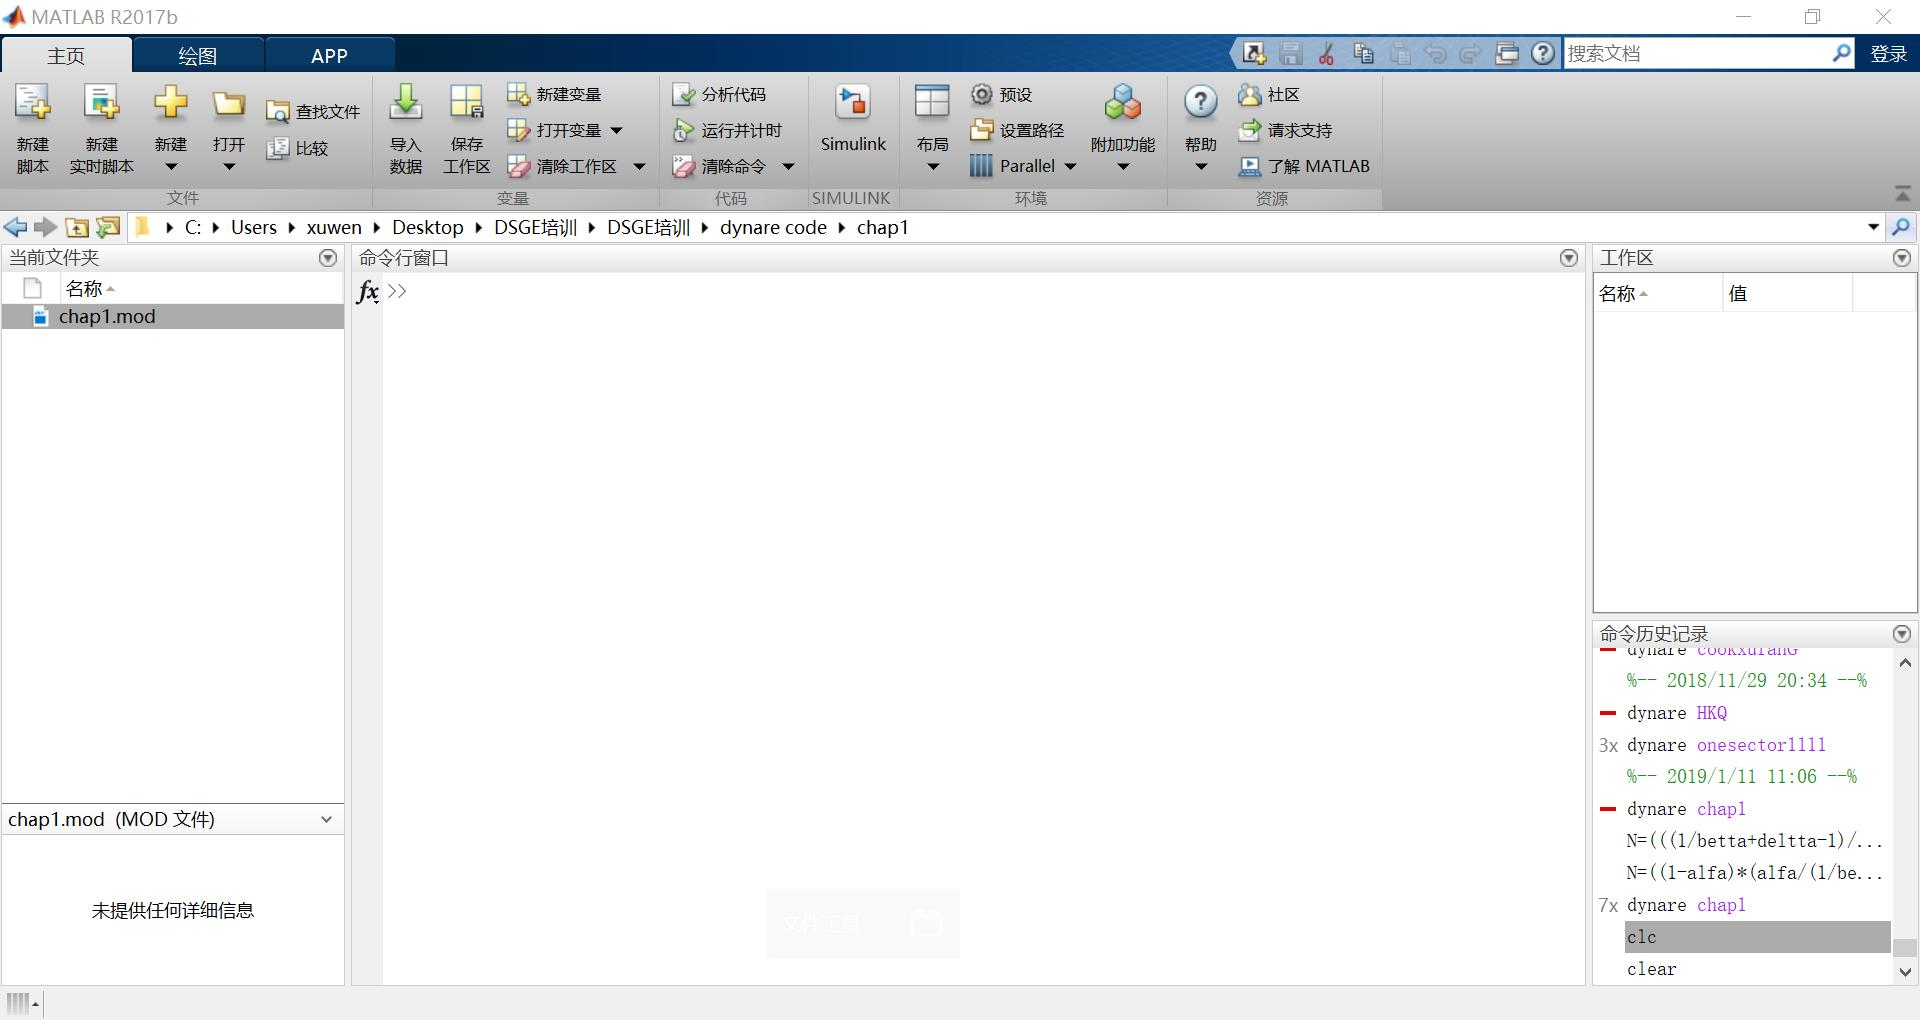
\includegraphics[width=0.8\linewidth]{FIG/matlab.jpg}
		
	\end{figure}
	
	In the command line window, we can see the cursor ">>", which means that matlab is ready and we can enter instructions here. After the cursor, we can input: add "+", subtract "-", multiply "*", divide "/", exponent "" and parentheses "()" and other commonly used mathematical and calculation symbols, functions and other commands .
	
	For example:
	\begin{figure}[htbp!]
		\centering
		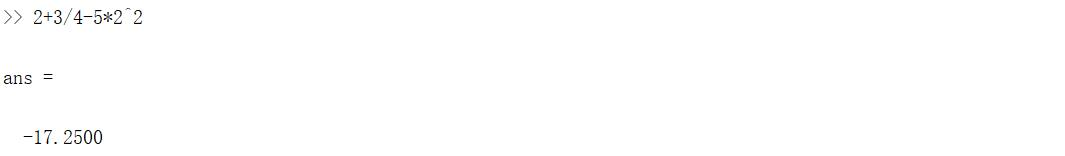
\includegraphics[width=0.8\linewidth]{FIG/calculate.jpg}
		
	\end{figure}
	
	In matlab, use "[]" to create a vector. Separate each element with a space or comma ",". Separate each line with a semicolon. E.g
	\begin{figure}[htbp!]
		\centering
		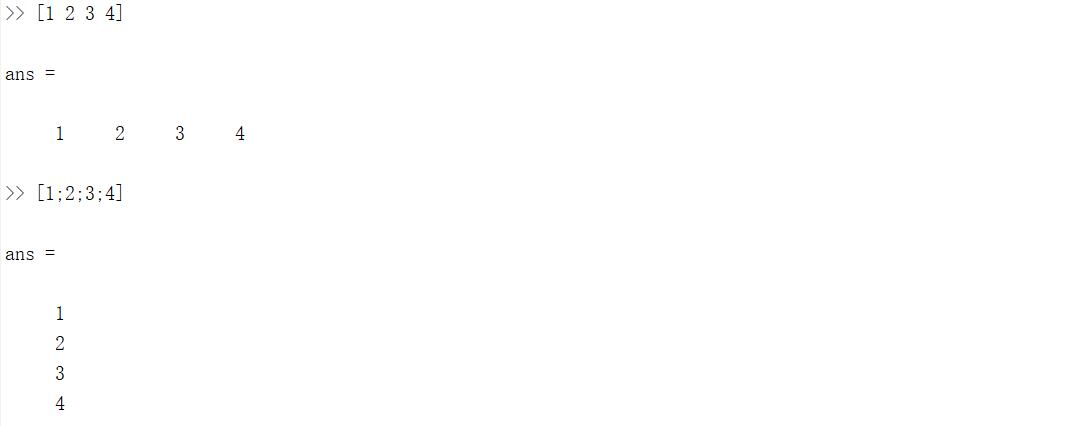
\includegraphics[width=0.8\linewidth]{FIG/vector.jpg}
		
	\end{figure}
	
	Note: (1) ans is the default result variable. We can also customize outcome variables. (2) Matlab follows Four Arithmetic Operations in Matlab.
	
	\section{Matrix Operations}
	
	Matrices or arrays are the basic elements of Matlab operations. A 1*1 matrix is a scalar or a single number, and a matrix with only one row or column is a row vector or a column vector. For example, the following basic operations on two matrices:
	\begin{figure}[htbp!]
		\centering
		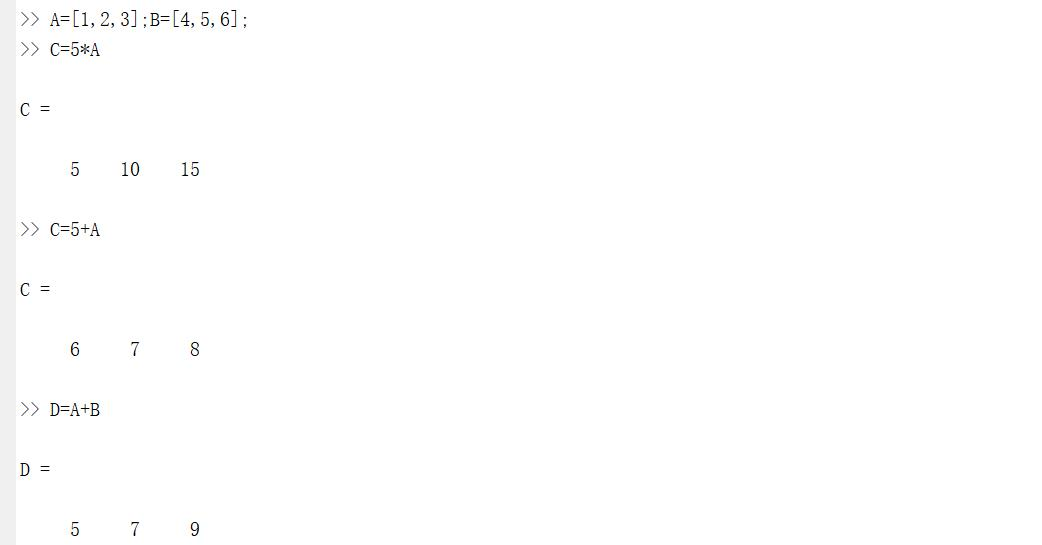
\includegraphics[width=0.8\linewidth]{FIG/matrixcalcu.jpg}
		
	\end{figure}
	
	Matlab can also perform inner product, dot product, dot division and exponentiation of matrices. The only requirement is that the vectors must be the same length. E.g
	\begin{figure}[htbp!]
		\centering
		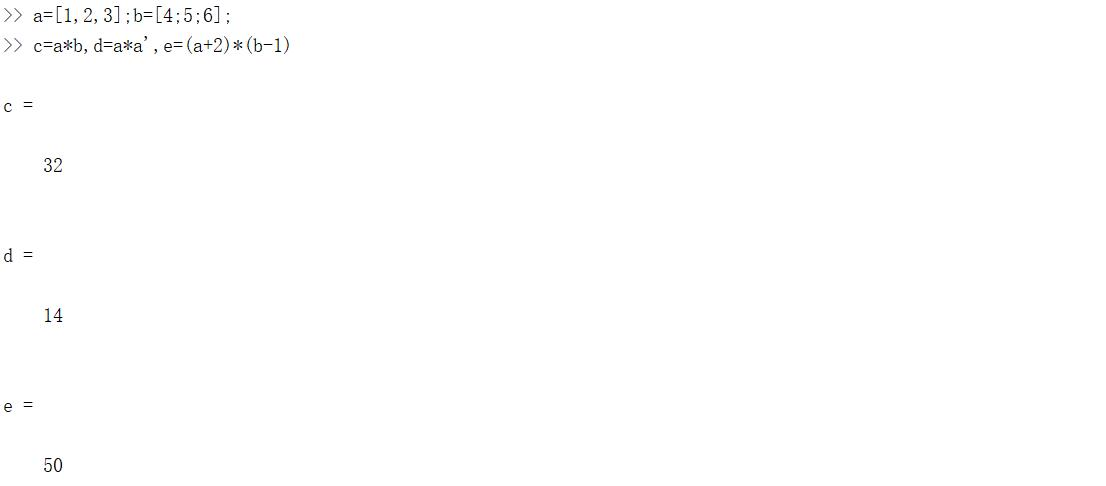
\includegraphics[width=0.8\linewidth]{FIG/innerprod.jpg}
		
	\end{figure}
	
	Dot multiply is as follows:
	\begin{figure}[htbp!]
		\centering
		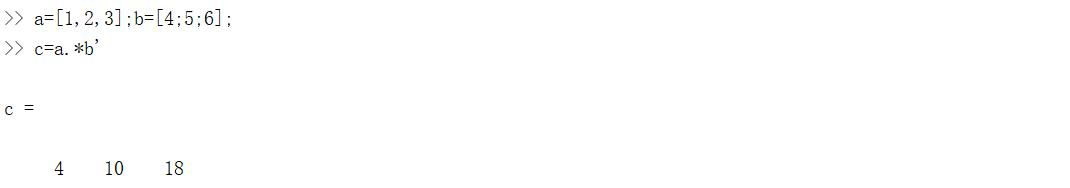
\includegraphics[width=0.8\linewidth]{FIG/dotprod.jpg}
		\centering
	\end{figure}
	
	\section{The colon usage}
	
	colon: A shortcut for creating a row vector. Also, colons can be used to view or extract certain elements of a vector. E.g
	\begin{figure}[htbp!]
		\centering
		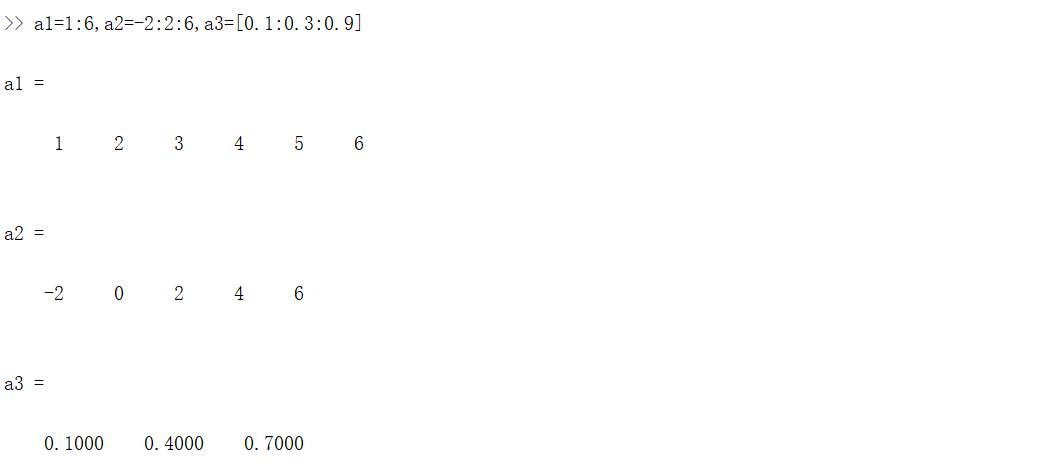
\includegraphics[width=0.8\linewidth]{FIG/colon.jpg}
		\centering
	\end{figure}
	
	Note: The usage of the colon is: start value: step size: end value.
	
	Extract elements 3-5 from a1:
	\begin{figure}[htbp!]
		\centering
		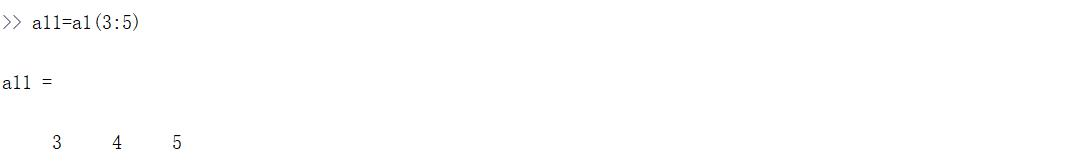
\includegraphics[width=0.8\linewidth]{FIG/extracting1.jpg}
		\centering
	\end{figure}
	
	Extract the 2,4,6th elements from a1:
	\begin{figure}[htbp!]
		\centering
		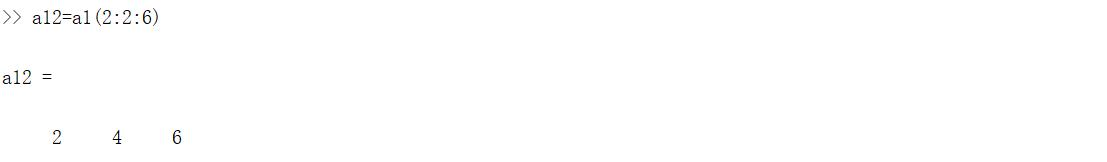
\includegraphics[width=0.8\linewidth]{FIG/extracting2.jpg}
		\centering
	\end{figure}
	
	\section{Figure}
	
	Matlab also has powerful drawing functions.
	
	The basic function for creating a 2D plot in Matlab is \textbf{plot(.)}. For example, make a graph of the parabola $Y=X^2$
	\begin{figure}[htbp!]
		\centering
		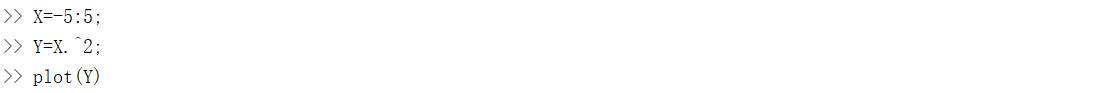
\includegraphics[width=0.8\linewidth]{FIG/Yplot.jpg}
		\centering
	\end{figure}
	
	get the following figure
	\begin{figure}[htbp!]
		\centering
		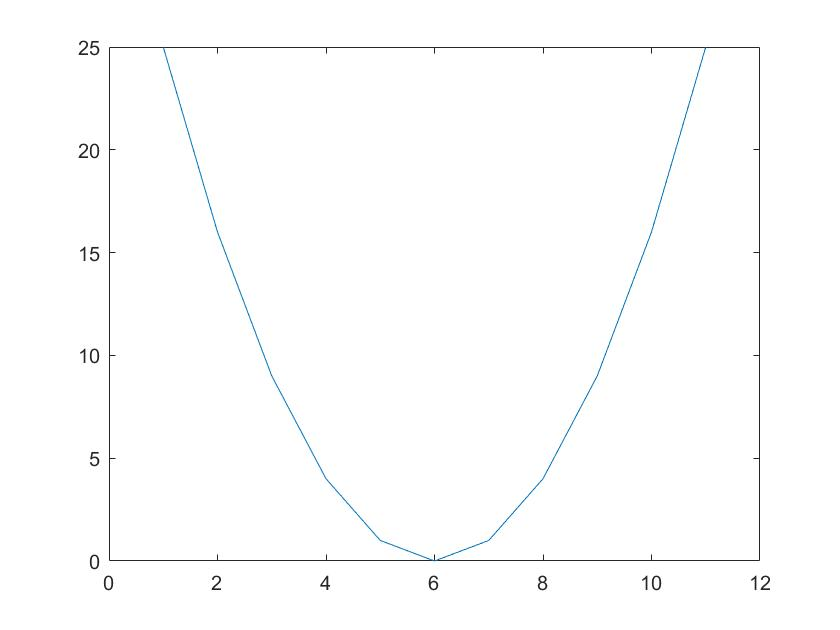
\includegraphics[width=0.8\linewidth]{FIG/Y.jpg}
		\centering
	\end{figure}
	
	If you want to display the range of X:
	\begin{figure}[htbp!]
		\centering
		
\includegraphics[width=0.8\linewidth]{FIG/XYplot.jpg}
		\centering
	\end{figure}
	
	get the following figure
	\begin{figure}[htbp!]
		\centering
		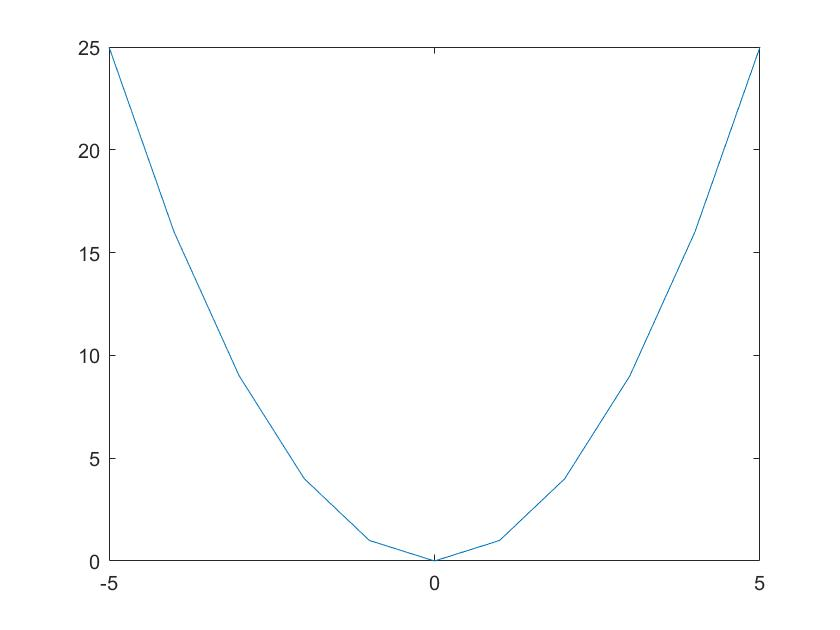
\includegraphics[width=0.8\linewidth]{FIG/XY.jpg}
		\centering
	\end{figure}
	
	You can also add the title of the figure, the title of the X-axis and the Y-axis in the above figure:
	\begin{figure}[htbp!]
		\centering
		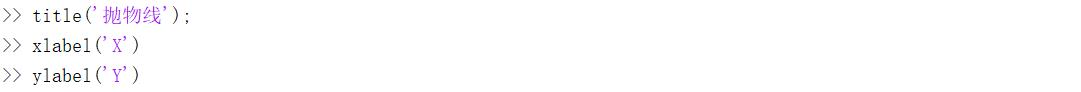
\includegraphics[width=0.8\linewidth]{FIG/title.jpg}
		\centering
	\end{figure}
	
	get the following figure
	\begin{figure}[htbp!]
		\centering
		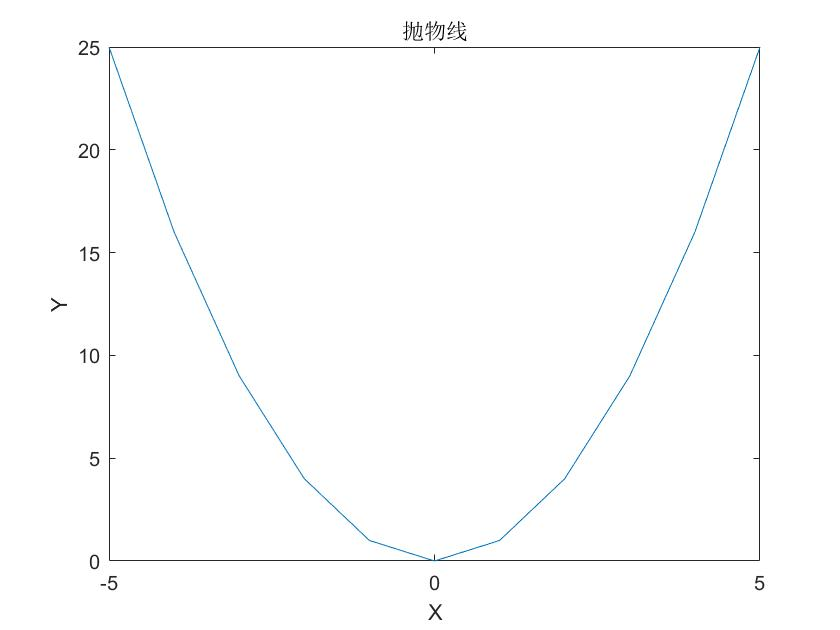
\includegraphics[width=0.8\linewidth]{FIG/XY1.jpg}
		\centering
	\end{figure}
	
	The function for 3D graphics is \textbf{plot3(.)}. Its basic usage is similar to plot, but with one more element. For example, to plot $Y=(XZ)^2$:
	\begin{figure}[htbp!]
		\centering
		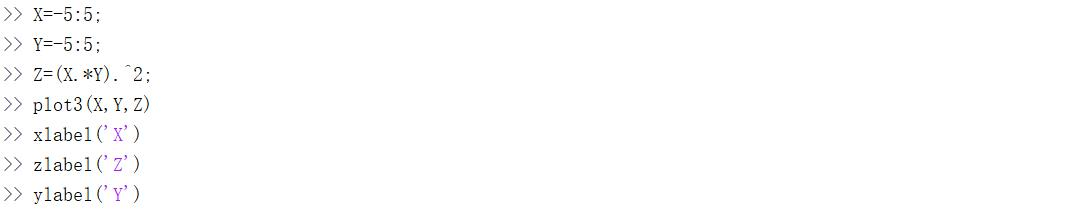
\includegraphics[width=0.8\linewidth]{FIG/3D.jpg}
		\centering
	\end{figure}
	
	get the following figure
	\begin{figure}[htbp!]
		\centering
		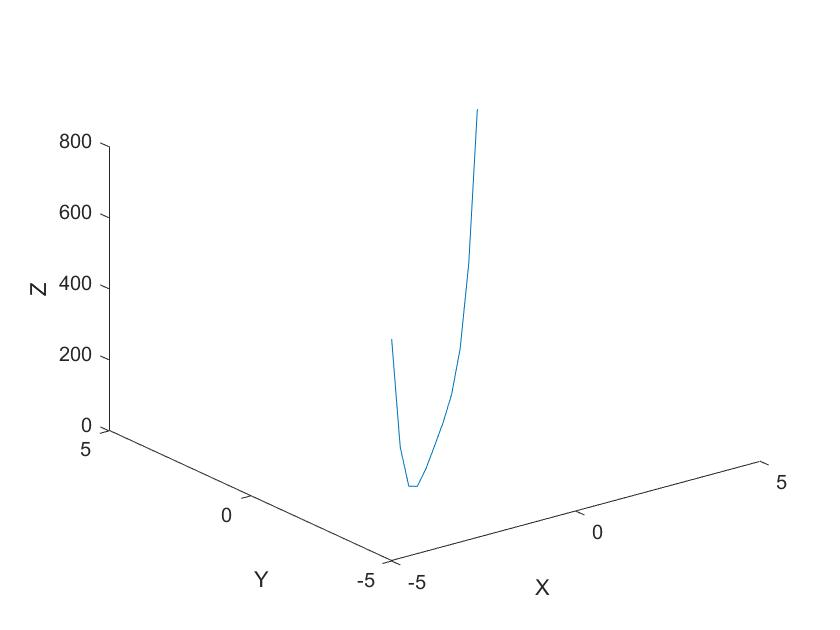
\includegraphics[width=0.8\linewidth]{FIG/3Dplot.jpg}
		\centering
	\end{figure}
	
	You can also use the \textbf{meshgrid(.)} function to make two-variable faces:
	\begin{figure}[htbp!]
		\centering
		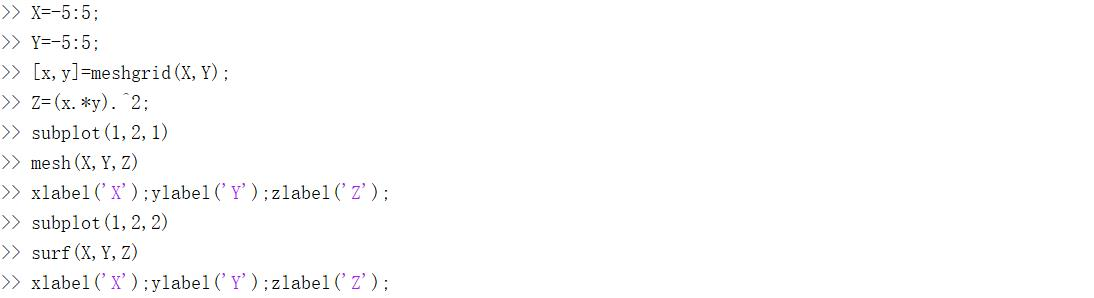
\includegraphics[width=0.8\linewidth]{FIG/surf.jpg}
		\centering
	\end{figure}
	
	get the following figure
	\begin{figure}[htbp!]
		\centering
		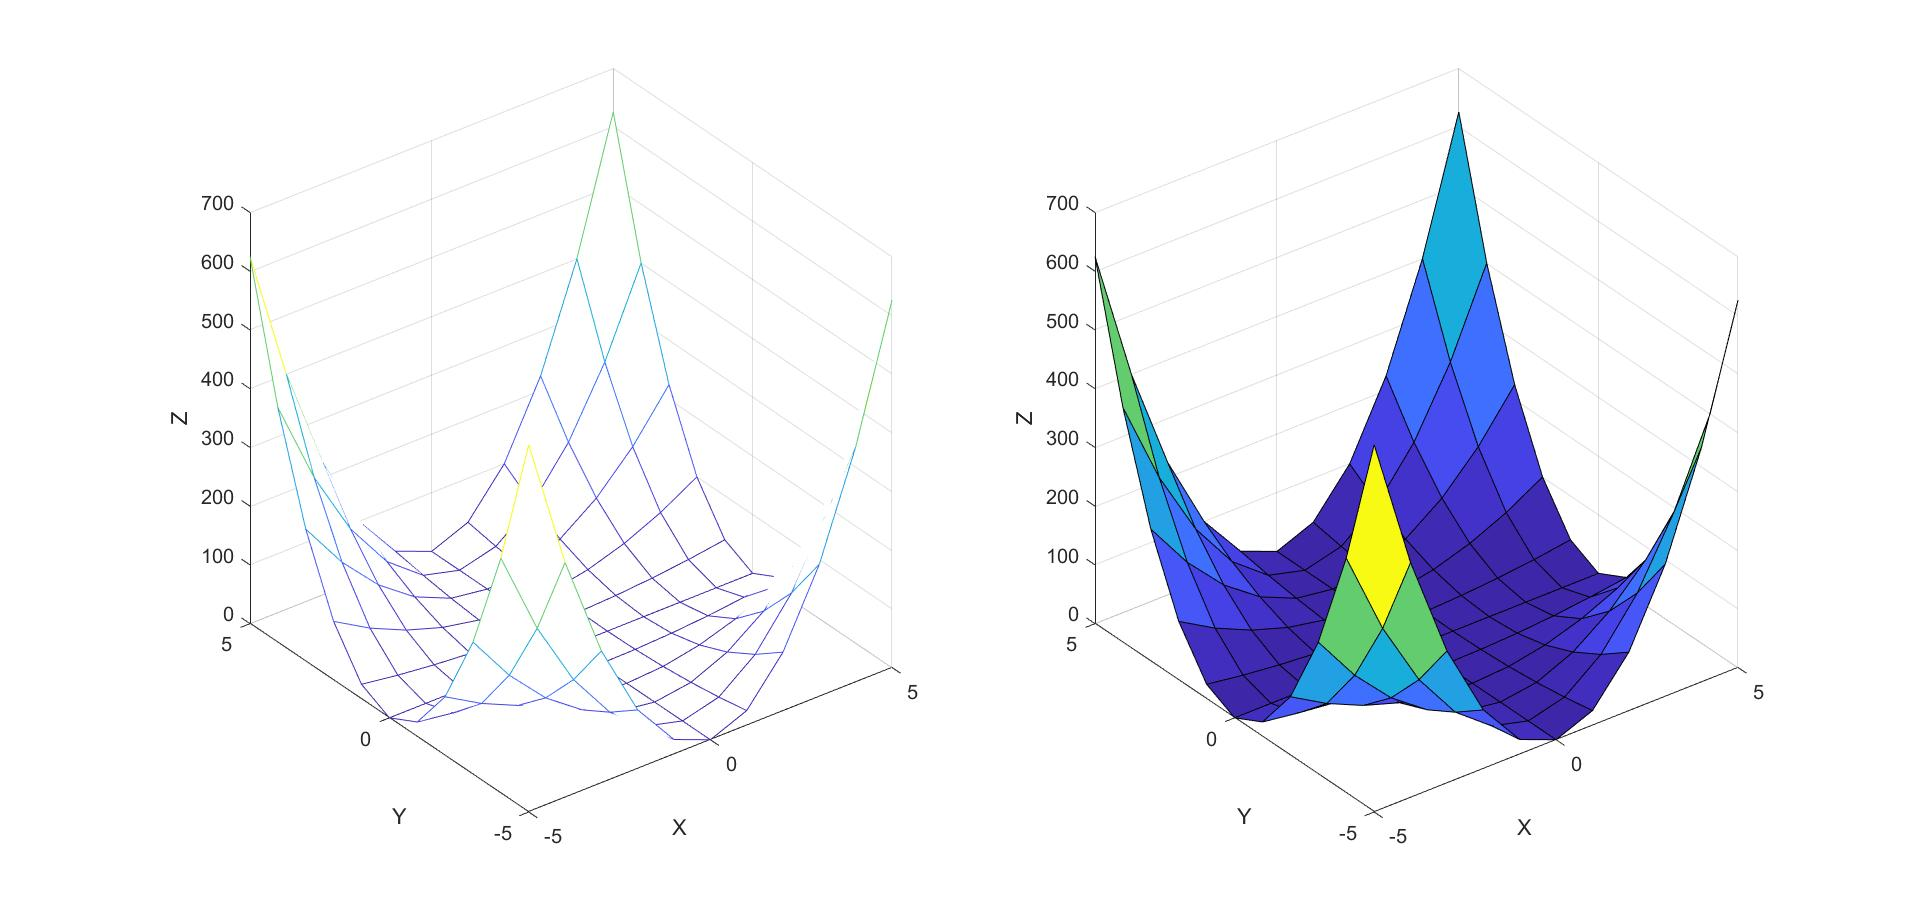
\includegraphics[width=0.8\linewidth]{FIG/surf1.jpg}
		\centering
	\end{figure}
	
	You can also draw their contours:
	
	\begin{figure}[htbp!]
		\centering
		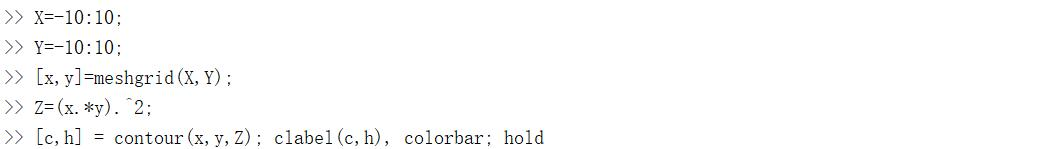
\includegraphics[width=0.8\linewidth]{FIG/contours}
		\centering
	\end{figure}
	
	get the following figure
	\begin{figure}[htbp!]
		\centering
		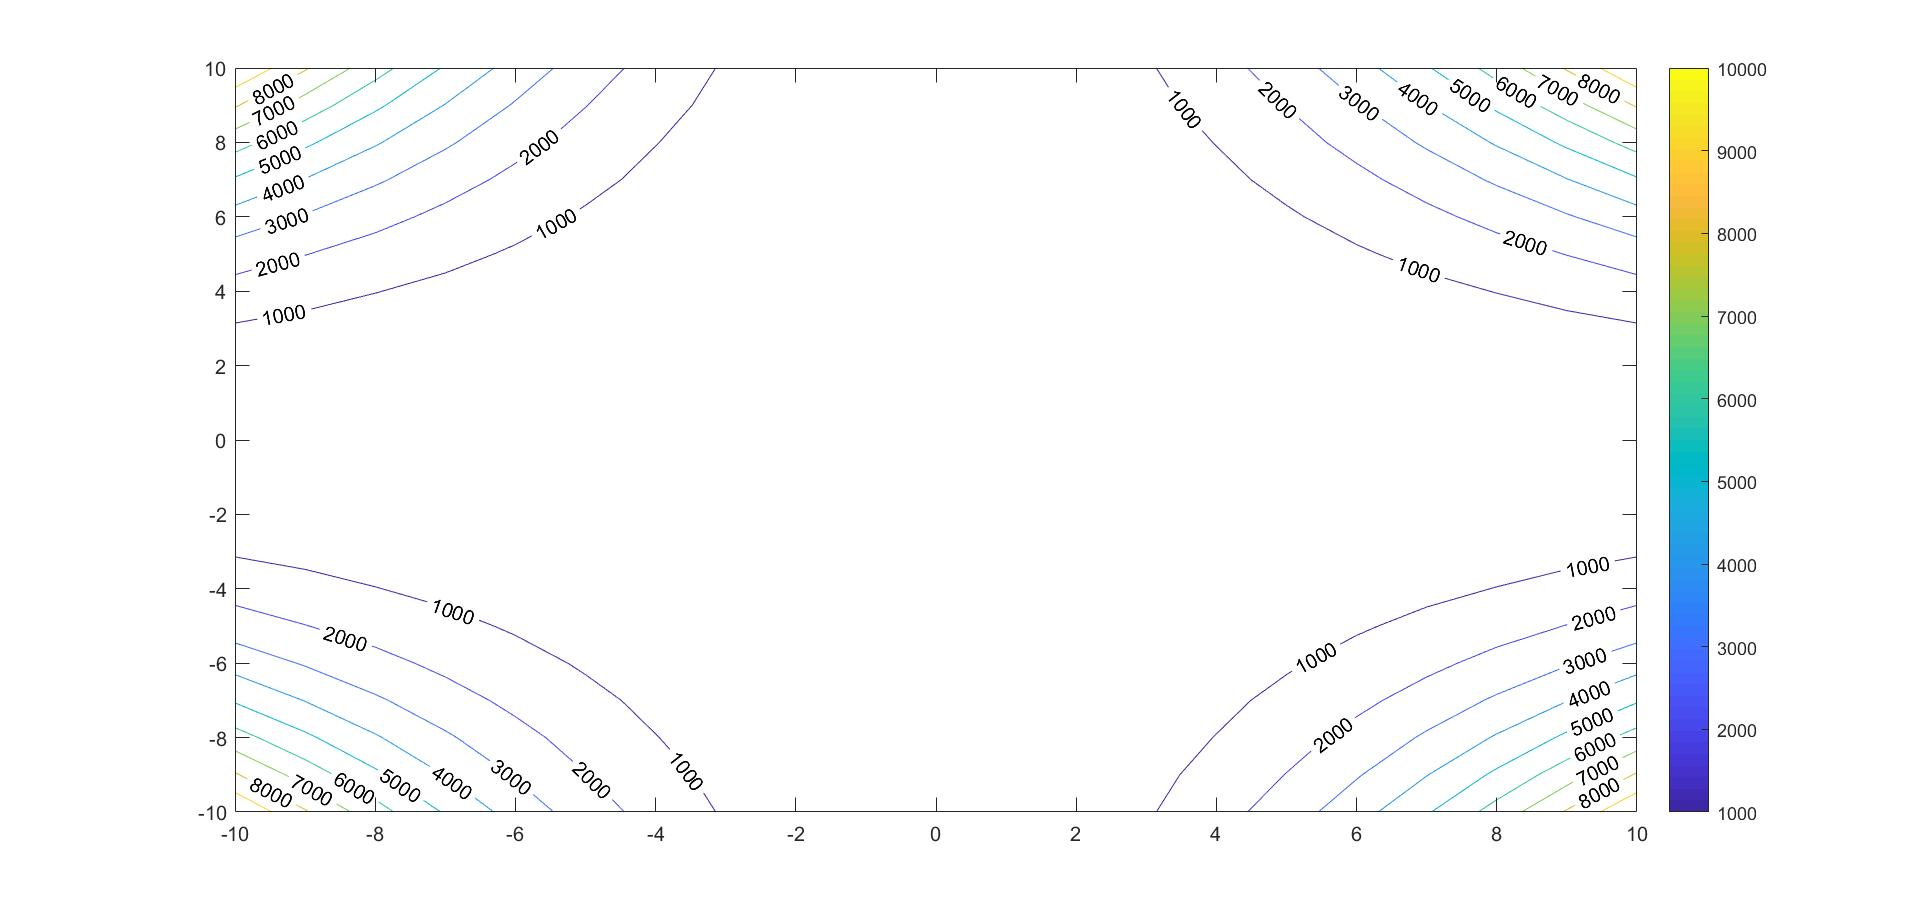
\includegraphics[width=0.8\linewidth]{FIG/contours1}
		\centering
	\end{figure}
	
	\section{Boolean expressions and loops}
	\subsection{Boolean expressions}
	When we try to execute a program under certain conditions, we first need to judge whether these conditions (or statements) are "true", these conditions are called "Boolean expressions".
	
	When we enter "2>1" in the command window, Matlab will output an integer "0" or "1", which tells us whether the entered expression is "true" (1 means "true", 0 means "false" ).
	\begin{figure}[htbp!]
		\centering
		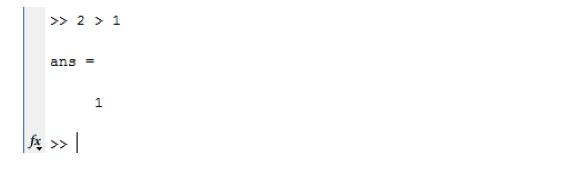
\includegraphics[width=0.8\linewidth]{FIG/Boolean}
		\centering
	\end{figure}
	
	In addition to this, there are some other relational notations:
	
	\begin{itemize}
		\item $>=$represents greater than or equal to;
		\item $<$represents strictly less than;
		\item $<=$represents less than or equal to
		\item $==$represents equal to;
		\item $~$represents 'False'.
	\end{itemize}
	
	We can also use "$\&$(and)" or "$\|$(or)" to connect several Boolean expressions, for example
	\begin{figure}[htbp!]
		\centering
		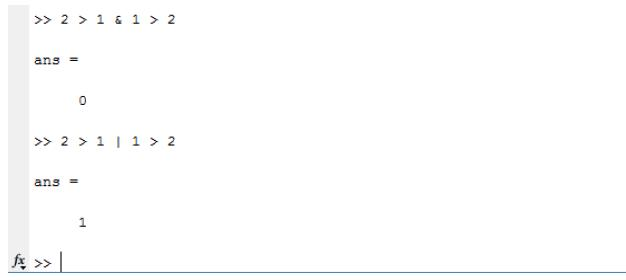
\includegraphics[width=0.8\linewidth]{FIG/connecting}
		\centering
	\end{figure}
	
	\subsection{Loop}
	
	For Matlab, a loop means executing some specified set of commands as long as a given Boolean statement is "true". There are three types of loops: while loop, for loop and if loop. They each have advantages and disadvantages. \textcolor{blue}{Note: We want to avoid using loops as much as possible, because loops are not matrix operations and they can make Matlab code run extremely slowly. }
	
	\begin{enumerate}
		\item The while loop executes \textbf{while} the set of commands when a Boolean statement is true.
		
		We first need to enter "while" to state the condition, and then add the command that needs to be executed. When we want to stop executing a command set, we enter "end". For example, to sum the integers from 0 to 10:
		
		\begin{figure}[htbp!]
			\centering
			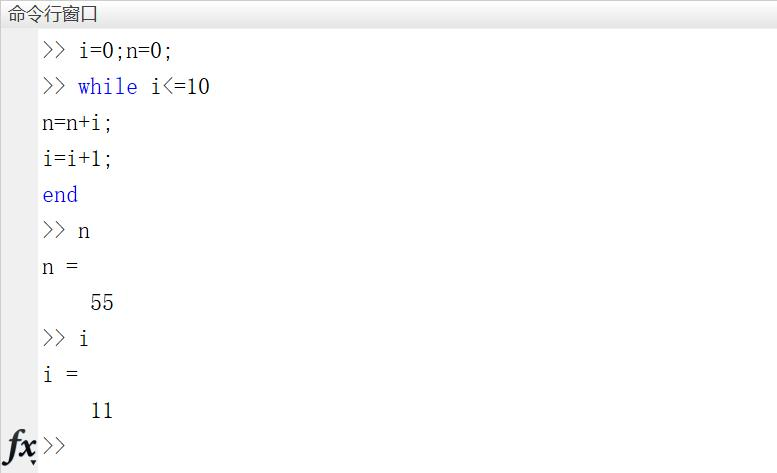
\includegraphics[width=0.8\linewidth]{FIG/integersum}
			\centering
		\end{figure}
		
		In the above example:
		
		i represents an integer variable, referring to the integer we use; n also represents an integer variable, referring to the result of our summation. At each step of the summation, the value of n is updated with the expression "$n=n+i$". So, how does Matlab read the while loop command?
		
		The first step is to read the right side of the Boolean statement, $n+i$, and then temporarily store its value in the workspace, for example, when i=0, n=0, then n+i=0, the value of 0 is will be temporarily stored in the workspace;
		
		The second step is to create a new variable, $n$, so that the new n is equal to the temporary value stored in the workspace. For example, the newly created n must be equal to the value of the workspace, that is, n=0;
		
		In the third step, when the Boolean statement in the while loop is "true", the first two steps are repeated, and the value of n is continuously upgraded until the final result is obtained, for example, when i=1, because in the second step n=0, so n+i=0+1=1, the value of 1 is stored in the workspace, and then the newly created n is equal to 1, repeat these steps, and finally get n=55.
		
		\item The if loop executes the set of commands that "\textbf{if}" is true for the given Boolean statement.
		
		Its grammatical structure is similar to that of a while loop: it starts with if and ends with end. For example, we continue to solve the sum of even numbers on the basis of the above integer sum.
		
		\begin{figure}[htbp!]
			\centering
			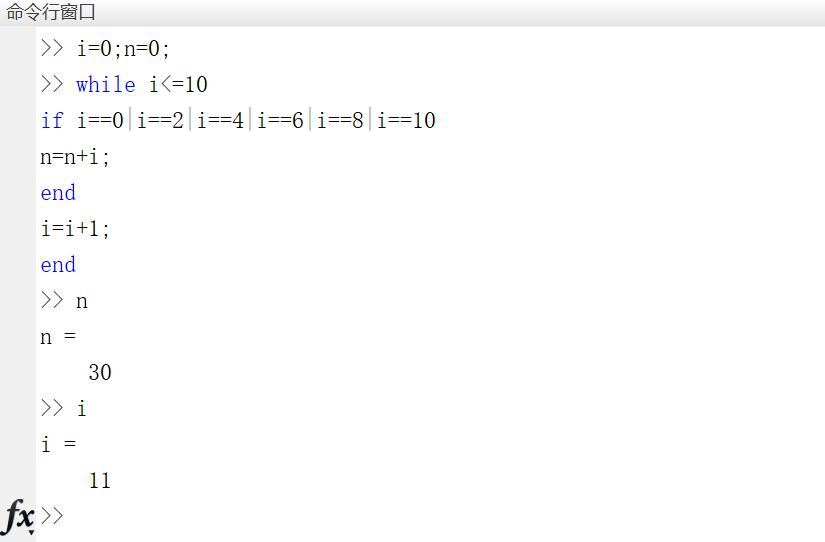
\includegraphics[width=0.8\linewidth]{FIG/evensum}
			\centering
		\end{figure}
		
	In the above example of adding even numbers, we added an if expression to the while loop. For each value of i, matlab must check the if expression, if i is even, then perform n=n+1 operation. \textbf{Note: Every Boolean expression requires an "end" at the end of the command set. }
	
	\item Strictly speaking, for loops are not like while and if loops, which execute a set of commands as long as the given Boolean expression is "true". It executes a given set of commands for an "indicator" value. For example, the summation of integers in while and if loops can be performed in a more compact way using a for loop by creating a vector of order n*1.
	
	First, calculate the sum of the integers
		
		\begin{figure}[htbp!]
			\centering
			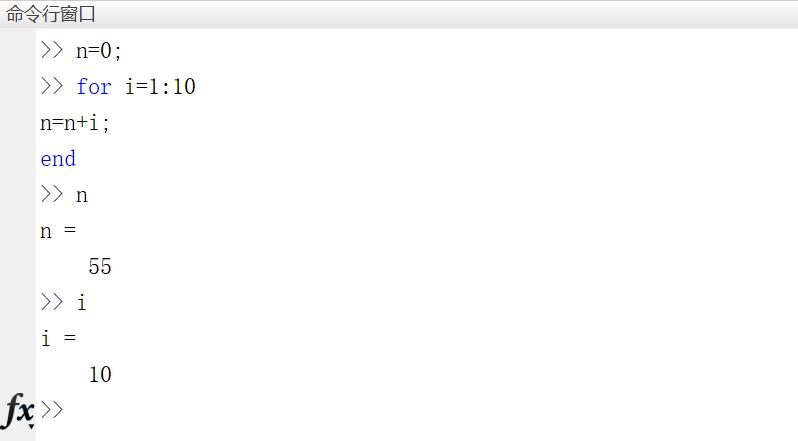
\includegraphics[width=0.8\linewidth]{FIG/vectorsum}
			\centering
		\end{figure}
	\end{enumerate}
	
Then, calculate the sum of the even numbers
	
	\begin{figure}[htbp!]
		\centering
		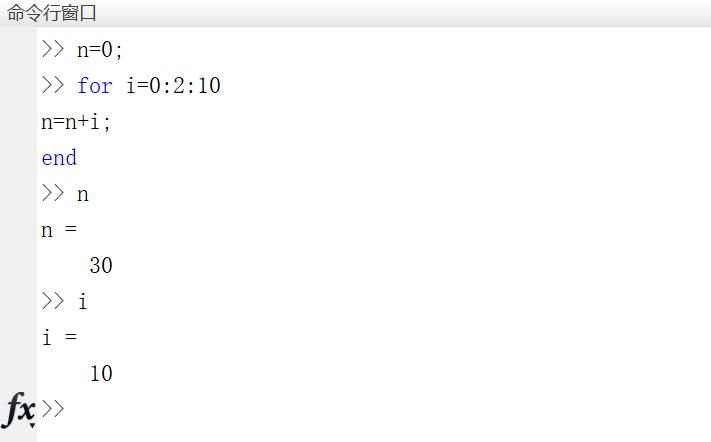
\includegraphics[width=0.8\linewidth]{FIG/vectorevensum}
		\centering
	\end{figure}
	
	The colon is used here, we can recall the previous explanation of the usage of the colon ":". i.e. "0:2:10" tells Matlab to create a vector from 0 to 10 with a step size of 2, i.e. 0,2,4,6,8,10.
	
	Note: Matlab's advantage is in matrix processing, and Boolean expressions can also be used for matrices.
	
	\section{Some useful built-in functions}
	
	\subsection{fzero}
	
	\textbf{fzero} is a Matlab built-in algorithm command for solving the roots of the nonlinear function $f(x)=0$.
	
	It has the following command formats:
	\begin{itemize}
		\item $x=fzero(fun,x0)$, where \textcolor{blue}{fun} represents the function name, and \textcolor{blue}{x0} represents the initial value.
		
		This command tries to find a point x such that $fun(x)=0$. At the root x, the function $fun(x)$ changes sign. Note: $fzero$ cannot solve the roots of functions such as $x^2$.
		
		Example 1: Roots near a point - Calculate the roots of the positive selection function $sin(x)=0$ near 3.
		
		\begin{lstlisting}[frame=shadowbox]
			fun = @sin; % Function name
			x0 = 3; % Initial value
			x = fzero(fun,x0)
		\end{lstlisting}
		
		$x=3.1416$
		
		Example 2: Roots in the interval - Find the roots of the cosine function on [0,1].
		
		\begin{lstlisting}[frame=shadowbox]
			fun = @cos; % Function name
			x0 = [1 2]; % Initial interval
			x = fzero(fun,x0)
		\end{lstlisting}
		
		$x=1.5708$
		
		Note: $cos(1)$ and $cos(2)$ have different signs.
		
		Example 3: Custom Function Rooting
		
		Solve for the roots of the function $f(x)=x^3-2x-5$.
		
		First, we have to write a custom function m file named f.m
		
		\begin{lstlisting}[frame=shadowbox]
			function y = f(x)
			y = x.^3-2*x-5;
		\end{lstlisting}
		
		Save the above f.m file to the current Matlab path. Then use the $fzero$ command to solve for roots around 2.
		
		\begin{lstlisting}[frame=shadowbox]
			fun = @f; % function
			x0 = 2; % initial point
			z = fzero(fun,x0)
		\end{lstlisting}
		
		$x=2.0946$
		
		Example 4: Root of a function with parameters
		\begin{lstlisting}[frame=shadowbox]
			myfun = @(x,c) cos(c*x);  % parameterized function
			c = 2;                    % parameter
			fun = @(x) myfun(x,c);    % function of x alone
			x = fzero(fun,0.1)
		\end{lstlisting}
		
		$x=0.7854$
		
		\item $x=fzero(fun,x0,options)$, where \textcolor{blue}{options} represents options.
		
		Example 5: The process of setting some image functions to display the solution
		
		Define functions and initial values
		
		\begin{lstlisting}[frame=shadowbox]
			fun = @(x)sin(cosh(x));
			x0 = 1;
		\end{lstlisting}
		
		Set the image options to show the process of the solution
		\begin{lstlisting}[frame=shadowbox]
			options = optimset('PlotFcns',{@optimplotx,@optimplotfval});
		\end{lstlisting}
		
		Run $fzero$:
		\begin{lstlisting}[frame=shadowbox]
			x = fzero(fun,x0,options)
		\end{lstlisting}
		
		\begin{figure}[htbp!]
			\centering
			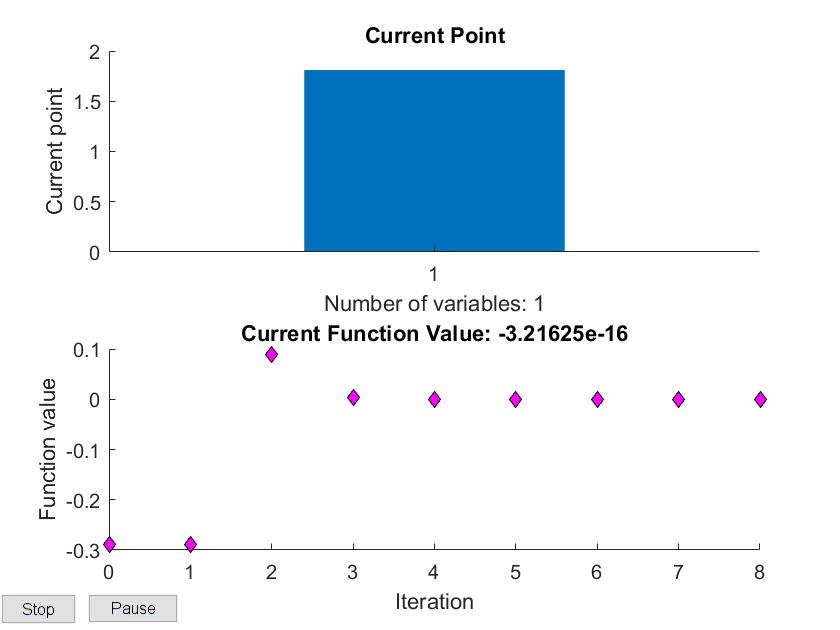
\includegraphics[width=0.8\linewidth]{FIG/options}
			\centering
		\end{figure}
		
		$x=1.8115$
		
		\item $[x,fval,exitflag,output] = fzero()$, the command structure displays the value of $fun(x)$ in $fval$, $exitflag$ displays the reason $fzero$ stopped, and $output$ contains information about the learned process.
		
		Example 6: 
		
		\begin{lstlisting}[frame=shadowbox]
			fun = @(x) exp(-exp(-x)) - x; % function
			x0 = [0 1]; % initial interval
			options = optimset('Display','iter'); % show iterations
			[x fval exitflag output] = fzero(fun,x0,options)
		\end{lstlisting}
	\end{itemize}
	
	\subsection{fsolve}
	
	$fsolve$ is Matlab's built-in solution for solving nonlinear systems of equations. To solve the following questions
	
	$$F(x)=0$$
	
	For x, $F(x)$ is the function value, expressed as a vector; x is a vector or matrix.
	
	The command format and description are:
	
	\begin{itemize}
		\item $x = fsolve(fun,x0)$ starts at x0 and tries to solve the equations fun(x) = 0, an array of zeros.
		\item $x = fsolve(fun,x0,options)$ solves the equations with the optimization options specified in options. Use $optimoptions$ to set these options.
		
		\item $x = fsolve(problem)$ solves problem, where problem is a structure described in Input Arguments. Create the problem structure by exporting a problem from Optimization app, as described in Exporting Your Work.
		
		\item $[x,fval] = fsolve()$, for any syntax, returns the value of the objective function fun at the solution x.
		
		
		\item $[x,fval,exitflag,output] = fsolve()$ additionally returns a value exitflag that describes the exit condition of fsolve, and a structure output with information about the optimization process.
		
		\item $[x,fval,exitflag,output,jacobian] = fsolve()$ returns the Jacobian of fun at the solution x.
		
		
	\end{itemize}
	
	Example 1: The system of equations is
	
	$$e^{-e^{-(x_1+x_2)}}=x_2(1+x_1^2)$$
	$$x_1cos(x_2)+x_2sin(x_1)=\frac{1}{2}$$
	
	First, convert the above formula into the form of $F(x)=0$
	$$e^{-e^{-(x_1+x_2)}}-x_2(1+x_1^2)=0$$
	$$x_1cos(x_2)+x_2sin(x_1)-\frac{1}{2}=0$$
	
	Then, write an m-file
	\begin{lstlisting}[frame=shadowbox]
		function F = root2d(x)
		
		F(1) = exp(-exp(-(x(1)+x(2)))) - x(2)*(1+x(1)^2);%where x represents a vector, containing two elements $x_1, x_2$, corresponding to x(1) and x(2) respectively
		F(2) = x(1)*cos(x(2)) + x(2)*sin(x(1)) - 0.5;
		
	\end{lstlisting}
	
	Save the above custom function as root2d.m in the current folder of Matlab.
	
	Solve the above system of equations starting at point [0,0]:
	\begin{lstlisting}[frame=shadowbox]
		
		fun = @root2d;
		x0 = [0,0];
		x = fsolve(fun,x0)
		
	\end{lstlisting}
	
	The result is
	
	Equation solved.
	
	fsolve completed because the vector of function values is near zero as measured by the value of the function tolerance, and
	the problem appears regular as measured by the gradient.
	
	
	x =
	
	0.3532  ~  0.6061
	
	\subsection{Parameter passing}
	
	Sometimes objective or constraint functions have parameters in addition to the independent variable. The extra parameters can be data, or can represent variables that do not change during the optimization. There are three methods of passing these parameters:
	
	\begin{itemize}
		\item Anonymous Functions
		
		\item Nested Functions
		
		\item Global Variables
		
		
	\end{itemize}
	
	Global variables are troublesome because they do not allow names to be reused among functions. It is better to use one of the other two methods.
	
	For example, suppose you want to minimize the function
	
	$$f(x)=(a-bx_1^2+x_1^4/3)x_1^2+x_1x_2+(-c+cx_2^2)x_2^2$$
	
	for different values of $a, b, and c$. Solvers accept objective functions that depend only on a single variable (x in this case). The following sections show how to provide the additional parameters $a, b, and c$. The solutions are for parameter values $a = 4, b = 2.1, and c = 4$ near $x_0 = [0.5 0.5]$ using $fminunc$.
	
	\textbf{Anonymous Functions}
	
	To pass parameters using anonymous functions:
	
	\begin{enumerate}
		\item Write a file containing the following code:
		\begin{lstlisting}[frame=shadowbox]
			
			function y = parameterfun(x,a,b,c)
			y = (a - b*x(1)^2 + x(1)^4/3)*x(1)^2 + x(1)*x(2) + ...
			(-c + c*x(2)^2)*x(2)^2;
		\end{lstlisting}
		
		\item Assign values to the parameters and define a function handle f to an anonymous function by entering the following commands at the MATLAB prompt:
		\begin{lstlisting}[frame=shadowbox]
			a = 4; b = 2.1; c = 4; % Assign parameter values
			x0 = [0.5,0.5];
			f = @(x)parameterfun(x,a,b,c);
		\end{lstlisting}
		
		\item Call the solver $fminunc$ with the anonymous function:
		\begin{lstlisting}[frame=shadowbox]
			[x,fval] = fminunc(f,x0)
		\end{lstlisting}
	\end{enumerate}
	
	The following output is displayed in the command window:
	
	Local minimum found.
	
	Optimization completed because the size of the gradient is less than the default value of the function tolerance.
	
	x =
	-0.0898  ~  0.7127
	
	fval =
	-1.0316
	
	\textbf{Nested Functions}   
	
	To pass the parameters for Equation 1 via a nested function, write a single file that
	
	\begin{itemize}
		\item Accepts a, b, c, and x0 as inputs
		
		\item Contains the objective function as a nested function
		
		\item Calls $fminunc$
	\end{itemize}
	
	Here is the code for the function file for this example:
	
	
	\begin{lstlisting}[frame=shadowbox]
		function [x,fval] =  runnested(a,b,c,x0)
		[x,fval] = fminunc(@nestedfun,x0);
		
		% Nested function that computes the objective function
		function y = nestedfun(x)
		y = (a - b*x(1)^2 + x(1)^4/3)*x(1)^2 + x(1)*x(2) +...
		(-c + c*x(2)^2)*x(2)^2;
		end
		end
	\end{lstlisting}
	
	The objective function is the nested function nestedfun, which has access to the variables a, b, and c.
	
	To run the optimization, enter:
	
	\begin{lstlisting}[frame=shadowbox]
		a = 4; b = 2.1; c = 4;% Assign parameter values
		x0 = [0.5,0.5];
		[x,fval] = runnested(a,b,c,x0)
		
	\end{lstlisting}
	
	\subsection{csolve}
	
	help csolve
	
	$function [x,rc] = csolve(FUN,x,gradfun,crit,itmax,varargin)$
	
	FUN should be written so that any parametric arguments are packed in to xp, and so that if presented with a matrix x, it produces a return value of same dimension of x.  The number of rows in x and FUN(x) are always the same.  The number of columns is the number of different input arguments at which FUN is to be evaluated.
	
	gradfun:  string naming the function called to evaluate the gradient matrix.  If this is null (i.e. just "[]"), a numerical gradient is used instead.
	
	crit:     if the sum of absolute values that FUN returns is less than this, the equation is solved.
	
	itmax:    the solver stops when this number of iterations is reached, with rc=4
	
	varargin: in this position the user can place any number of additional arguments, all of which are passed on to FUN and gradfun (when it is non-empty) as a list of arguments following x.
	
	rc:       0 means normal solution, 1 and 3 mean no solution despite extremely fine adjustments in step length (very likely a numerical problem, or a discontinuity). 4 means itmax termination.
	
	
	\subsection{broyden}
	
	help broyden
	
	\textbf{broyden}
	
	Computes root of function from $R^n$ to $R^n$ using Broyden's inverse update method with backstepping.
	
	Usage
	
	$[x,fval,fjacinv] = broyden(f,x,varargin)$
	
	Input
	
	f         : function of form fval=f(x,varargin)
	
	x         : n.1 initial guess for root
	
	varargin  : optional parameters passed to f
	
	Output
	
	x         : n.1 root of f
	
	fval      : n.1 function value estimate
	
	fjacinv   : n.n inverse Jacobian estimate
	
	Options
	
	maxit     : maximum number of iterations (100)
	
	tol       : convergence tolerance (1e-10)
	
	maxsteps  : maximum number of backsteps (25)
	
	showiters : display results of each iteration (1)
	
	initb     : an initial inverse Jacobian approximation matrix ([])
	
	initi     : if initb empty, and initi is 1, use identity matrix to initialize if initi is 0, use numerical Jacobian (0)
	
	\section{Custom function}
	
	Entering commands directly in the command window can be problematic, especially if the program is long. Matlab also provides us with another code editing window - the script window. A series of commands can be entered in the script window, and we save these commands as matlab default files - m files (the reason why they are called m files is because the suffix of the file is .m).
	
	If the m file does not require external input, these commands can be run, then the file are called scripts.
	
	Another m-file is a function. A function file's commands require external input to run.
	
	Note: The name of the m file should be the same as the name of the function. We may want to use a custom function to solve the steady state of the DSGE model.
	
	For example, define a simple parabolic function $f(x)=x^2$. where x is the external input and the function f returns the value of $x^2$.
	
	First of all, we need to create a new script, which is the m file:
	\begin{figure}[htbp!]
		\centering
		\includegraphics[width=0.8\linewidth]{FIG/newscript}
		\centering
	\end{figure}
	
	Define the function:
	\begin{figure}[htbp!]
		\centering
		\includegraphics[width=0.8\linewidth]{FIG/function1}
		\centering
	\end{figure}
	
	To create a function file:
	
	In the first step, we need to start the command with "\textbf{function}" on the first line, followed by the output of the function (in the above example, y is the output), which is equal to the function name ("sqr" in the example ) and input(x).
	
	The second step is to write our related commands. In the example, the output y is assigned a value, and the assignment is the square of the input x.
	
	More complex functions may have multiple inputs and multiple outputs, or different types of inputs and outputs (eg, matrices, characters, or other functions).
	
	In order to call the sqr.m file, we just need to enter in the matlab command window:
	
	\begin{figure}[htbp!]
		\centering
		\includegraphics[width=0.8\linewidth]{FIG/sqr}
		\centering
	\end{figure}
	
	In addition, we can also write simple functions directly in the command window of matlab using the so-called "in-line" functions:
	\begin{figure}[htbp!]
		\centering
		\includegraphics[width=0.8\linewidth]{FIG/inlinefunction}
		\centering
	\end{figure}
	
	The first line of command is to define a function. The left side of the equal sign is the function name "$sqr\_inline$", and the right side of the equal sign is "@(x)", which tells Matlab that we define a function whose input is x, followed by telling Matlab the The return value (output value) of the function $x^2$. For example, we call the function "$sqr\_inline$" with an input of 3 and a return value of 9.
	
	Next, let's write a more complex function file: calculate the sum of the first n integers, where the integer n is the input to the function.
	
	\begin{figure}[htbp!]
		\centering
		\includegraphics[width=0.8\linewidth]{FIG/sumintegers}
		\centering
	\end{figure}
	
	Save the above file, the file name is the function name: $sum\_integers.m$. Now, let's call this function to calculate the sum of integers.
	
	\begin{figure}[htbp!]
		\centering
		\includegraphics[width=0.8\linewidth]{FIG/sumintegersresults}
		\centering
	\end{figure}
	
	Some commonly used functions are also built in Matlab.
	
	1. The minimum value of the function
	
	For example, we want to solve for x that minimizes the parabola $f(x)=x^2$. At this point, we can use Matlab's built-in minimization function "\textbf{fminunc}".
	
	\begin{figure}[htbp!]
		\centering
		\includegraphics[width=0.8\linewidth]{FIG/fminunc}
		\centering
	\end{figure}
	
	In the above example, the first line defines the in-line function f first. The second line of commands uses the function "fminunc" to solve for the value of x that minimizes the function f. The function "fminunc" has two input elements: \textbf{minimize objective function f} and \textbf{initial guess of x1}.
	
	For more information on the function "fminunc", see the help file or online resources. For more optimization functions in Matlab, please refer to the Matlab help documentation or online resources.
	
	\begin{figure}[htbp!]
		\centering
		\includegraphics[width=0.8\linewidth]{FIG/helpfminunc}
		\centering
	\end{figure}
	
	2. Roots-solving 
	
	Another commonly used function is solving the roots of an equation - finding the value of x such that the function f(x)=0. A commonly used root function is "fsolve": for example, solve the root of the function $f(x)=x^2-2$	
	\begin{figure}[htbp!]
		\centering
		\includegraphics[width=0.8\linewidth]{FIG/fsolve}
		\centering
	\end{figure}
	
	It should be noted that general-purpose function operations are not matrix operations, so Matlab is not good at this. However, Matlab is good at doing linear operations, so if we can convert nonlinear equations into linear equations, then matlab can still do the job well. For example, in the above example, although we ask to solve the roots of $f(x)=x^2-2$, matlab solves the roots of $x-\sqrt{2}=0$, so we see the final result The output is only 1.4142.
	
	Of course, in order to solve the roots of linear equations, Matlab also has built-in many other root functions, please refer to Matlab's help documentation or online resources.
	
	\section{Read data}
	
	Above, we have tried some commands to create data files. However, in practice, we often need to read external data files directly, especially non-m files and mat files. For example, we want to read the most common excel files. Fortunately, Matlab can read excel files directly.
	
	For example, our excel file is named "template.xlsx", which is read with matlab.
	
	\begin{figure}[htbp!]
		\centering
		\includegraphics[width=0.8\linewidth]{FIG/excel}
		\centering
	\end{figure}
	
	where Y represents the variable name saved in the read file, xlsread represents the excel file reading function, and template.xlsx (or filename.xls) represents the excel data file. It should be noted that the data file should be enclosed in single quotation marks under the English characters.
	
	
	
	
\end{document}
